\documentclass{scrbook}

\usepackage{theseinalco}
\usepackage{ebgaramond-maths}
\usepackage{blindtext}

\usepackage{rotating}
\usepackage{polyglossia}
\setmainlanguage{french}
\usepackage{ctex}
\usepackage{subcaption}
\usepackage{tablefootnote}
\usepackage{makecell}
\usepackage{multirow}
\usepackage{booktabs}
\usepackage{fontspec}
\setmainfont{Charis SIL}
\setCJKmainfont{SIMSUN.ttc}
\usepackage{xspace}
\usepackage{graphicx}
\usepackage{longtable}
\usepackage{colortbl}
\usepackage{xcolor}
\usepackage[colorlinks=true, linkcolor=blue, anchorcolor=blue, citecolor=blue]{hyperref}%true表示打印时也显示出颜色,false表示颜色在打印时不会显示出来
\usepackage{pdflscape}
\usepackage{appendix}

\usepackage[style=langsci-unified]{biblatex}
\addbibresource{MasterRef.bib}
\DefineBibliographyExtras{french}{\renewcommand*\mkbibnamefamily[1]{#1}}
\DeclareFieldFormat*{titlecase}{#1}
\DeclareNameAlias{default}{family-given}
\renewcommand*{\multinamedelim}{\addspace\&\addspace}
\DefineBibliographyStrings{french}{editors = {éds\adddot}}
\DeclareFieldFormat{type}{\mkbibparens{\bibstring{#1}}}

%subsubsection下继续编号
\newcounter{c}[subsubsection]
\newcommand{\stpc}[1]{\stepcounter{#1}}
%\stpc{c}\paragraph{(\arabic{c})}
%\newcommand{\para}[1]{\stpc{c}\paragraph{(\arabic{c})}}
%可以新定义\para,但是不能重新定义\paragraph,似乎是因为计算量过大,这里不取重新定义,因为原代码\paragraph的蓝色字体比较醒目。

\newcommand{\bolang}{\textasciitilde}
\newcommand{\difwenbai}{couches archaïque et récente\xspace}
\newcommand{\diflaoxin}{sociolectes âgé et jeune\xspace}
\newcommand{\iso}{syllabes isolées\xspace}
\newcommand{\illustre}{Les exemples sont illustrés dans la table\xspace}
\newcommand{\termyyx}[1]{\textbf{#1}}
\newcommand{\isowenbai}{Il existe des \difwenbai sur certaines \iso.\xspace}
\newcommand{\isolaoxin}{Il existe des \diflaoxin sur certaines \iso.\xspace}
\newcommand{\exclure}[1]{Il faut d'abord exclure les syllabes #1 avant d'identifier les \difwenbai}

%章节名称
%\subsection{\MakeCapital{\difwenbai}}
%\subsection{\MakeCapital{\difwenbai} (\iso)}
%\subsection{\MakeCapital{\diflaoxin}}
%\subsection{\MakeCapital{\diflaoxin} (\iso)}

%\stpc{c}\paragraph{(\arabic{c})}
%Les syllabes \termyyx{} ont pour couche archaïque et pour couche récente , e.g. 
%\illustre \ref{tab:}.
%系统文白Selon \textcite[XXX]{XXX}, il existe des différences systématiques entre les \difwenbai. \illustre \ref{tab:}.
%孤立文白\isowenbai \illustre \ref{tab:}.
%系统老新Selon \textcite[XXX]{XXX}, il existe des différences systématiques entre les \diflaoxin. \illustre \ref{tab:}.
%孤立老新\isolaoxin \illustre \ref{tab:}.

%表格名称
%Les \difwenbai du XXX
%Les \difwenbai du XXX (\iso)
%Les \diflaoxin du XXX
%Les \diflaoxin du XXX (\iso)

\title{Constitution d'une base de données lexicales des langues sinitiques et contribution à l'étude de leur phylogénie}
\author{YIN Yuanhao (22100358)}
\preauthor{présenté par}

\logo{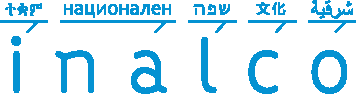
\includegraphics[scale=.8]{inalco-logo-color}}
\universite{institut national des langues et civilisations orientales}
%\ecoledoctorale{École doctorale n\textsuperscript{o}265:\quad \textit{Langues, Littératures et Sociétés du monde}}
%\unite{Langues et civilisations (\textsc{umr} 0000)}
\diplome{Mémoire}

\date{soutenance prévue le 3 juillet 2023}%Soutenue publiquement le
\discipline{Sciences du Language (M2)

Parcours : Linguistique : langues, terrains, variations, typologie}
\grade{pour obtenir le grade de Master de l'\textsc{inalco}}
\direction{Mémoire dirigé par:}
\directeur{M.}{Guillaume}{Jacques}{Directeur de recherches, CRLAO (EHESS, INALCO, CNRS) \& EPHE, PSL}
\directeur{M\textsuperscript{me}}{Christine}{Lamarre}{Professeure des universités, CRLAO (EHESS, INALCO, CNRS)}

\jury{M.}{Guillaume}{Jacques}{Directeur de recherche, CRLAO (EHESS, INALCO, CNRS) \& EPHE, PSL}
\jury{M\textsuperscript{me}}{Christine}{Lamarre}{Professeure des universités, CRLAO (EHESS, INALCO, CNRS)}
\jury{M.}{Thomas}{Pellard}{Chargé de recherche, CRLAO (EHESS, INALCO, CNRS)}

\onehalfspacing% interligne

\begin{document}
\maketitle
\begin{sloppypar}

\frontmatter
\chapter{Résumé}
%\blindtext
Ce mémoire a pour but de tester si l'exclusion des emprunts influencerait les résultats phylogénétiques des langues sinitiques et d'obtenir une impression préliminaire de ces résultats. Au niveau de la méthodologie, on discute de la connotation du terme traditionnel dans la dialectologie chinoise ``wen-bai'' et de ses insuffisances, sur la base du quoi sont généralisés les critères généraux et concrets de la stratification de 19 langues sinitiques d'une base de données déjà établie. Au niveau des données, ces critères précédents sont employés pour annoter les couches des syllabes des mots de cette base de données pour distinguer les mots hérités et les emprunts, afin d'obtenir deux séries de données avec ou sans emprunts. Au niveau de la technique, on applique principalement la méthode d'UPGMA, la méthode d'NJ et la méthode du maximum de parcimonie à ces deux séries de données pour discuter les résultats phylogénétiques et leurs inspirations. On trouve que l'exclusion des emprunts n'influence pas beaucoup les topologies générales des arbres UPGMA et NJ, mais le fait pour la méthode du maximum de parcimonie. Les résultats phylogénétiques confirment dans une certaine mesure la classification traditionnelle des langues sinitiques et révèlent en même temps certains points apparemment anormaux. Il faut bien veiller à la méthodologie pendant les enquêtes sur le terrain pour collecter les données pertinentes et au phénomène de la nativisation des emprunts qui cause des emprunts non détectables, tous deux risquant d'induire en erreur les résultats phylogénétiques. Dans le futur, plus de travaux profonds méritent d'être effectués pour approfondir la phylogénie des langues sinitiques.
\paragraph{mots-clés:} langues sinitiques, stratification, phylogénie

\chapter{Remerciements}
%\blindtext
J'en profite pour remercier M. Guillaume Jacques, mon directeur de mémoire, de m'avoir aidé à choisir ce sujet de mémoire et de m'avoir dirigé au niveau théorique et pratique du début à la fin.

Je remercie Mme Christine Lamarre, la première professeure de l'INALCO que j'ai contactée et ma deuxième directrice de mémoire, de m'avoir accepté dans le domaine de la linguistique et de m'avoir initié à la syntaxe du chinois pendant ma période du Master. 

Je remercie M. Thomas Pellard de m'avoir soutenu au niveau de différents aspects techniques pendant la rédaction de ce mémoire.

Je remercie M. Johann-Mattis List, sur l'article duquel j'ai basé mon mémoire, de m'avoir fourni la base de données initiale et de m'avoir aidé à détecter des erreurs après que j'avais fini l'annotation.

Je remercie SWUPL, mon université de licence en Chine d'avoir continué de me fournir les ressources de la bibliothèque en ligne, ce qui a facilité la recherche des littératures pour mon mémoire.

Enfin, je remercie tous les autres professeurs et camarades et ma famille de m'avoir accompagné et inspiré dans mes études du Master.

\mainmatter
\chapter{Introduction}
La classification traditionnelle populaire établie par \textcite{li1987atlas} et \textcite{xiong2012atlas} divise les langues sinitiques en dix groupes : Mandarin (官話), Jin (晉語), Wu (吳語), Min (閩語), Hakka (客家話), Yue (粵語), Xiang (湘語), Gan (贛語), Hui (徽語) et Pinghua et Tuhua (平話和土話), en séparant trois nouveaux groupes des sept groupes traditionnels : Jin, Hui et Pinghua et Tuhua. Les deux critères primaires de leur classification sont (1) les formes actuelles des initiales voisées du chinois moyen dans les variantes d'aujourd'hui ; et (2) l'appartenance actuelle du tonème rentrant du chinois moyen dans les variantes d'aujourd'hui. Ces deux critères portent trois traits : (1) ils sont phonétiques/phonologiques ; (2) ils comptent sur la rétention d'une certeine catégorie phonologique d'une langue ancestrale dans les langues actuelles ; et (3) ils ne tiennent pas en compte la stratification des langues. 

Cependant, sous l'introduction de la perspective de la phylogénie de la biologie de l'évolution, ces deux critères ne conviennent pas à la construction d'un arbre phylogénétique : d'abord, les changements phonétiques sont tellement fréquents qu'ils peuvent arriver d'une façon récurrente dans différentes langues ; ensuite, il faut compter sur les innovations communes plutôt que les rétentions communes pour déterminer quelles langues constituent un clade, càd. un groupe de langues qui partagent le \textbf{dernier ancêtre commun (DAC)} ; enfin, il est important d'identifier les couches héritées par les langues pour assurer la pertinence des résultats. Ainsi, il vaut mieux que les critères pour la classification phylogénétique soient établis comme : (1) lexicaux, surtout sur la base des mots de base, puisque ceux-ci sont plus stables que les traits phonétiques ; (2) se servant des innovations communes lexicales pour la classification ; et (3) identifiant les couches héritées des langues. \textcite{sagart2011classifying} a appliqué ces trois crtières pour essayer de proposer un arbre phylogénétique (figure \ref{fig:sagart_class}) mais d'une façon assez simple, parce qu'il n'a pas utilisé les méthodes informatiques.

\begin{figure}
\centering
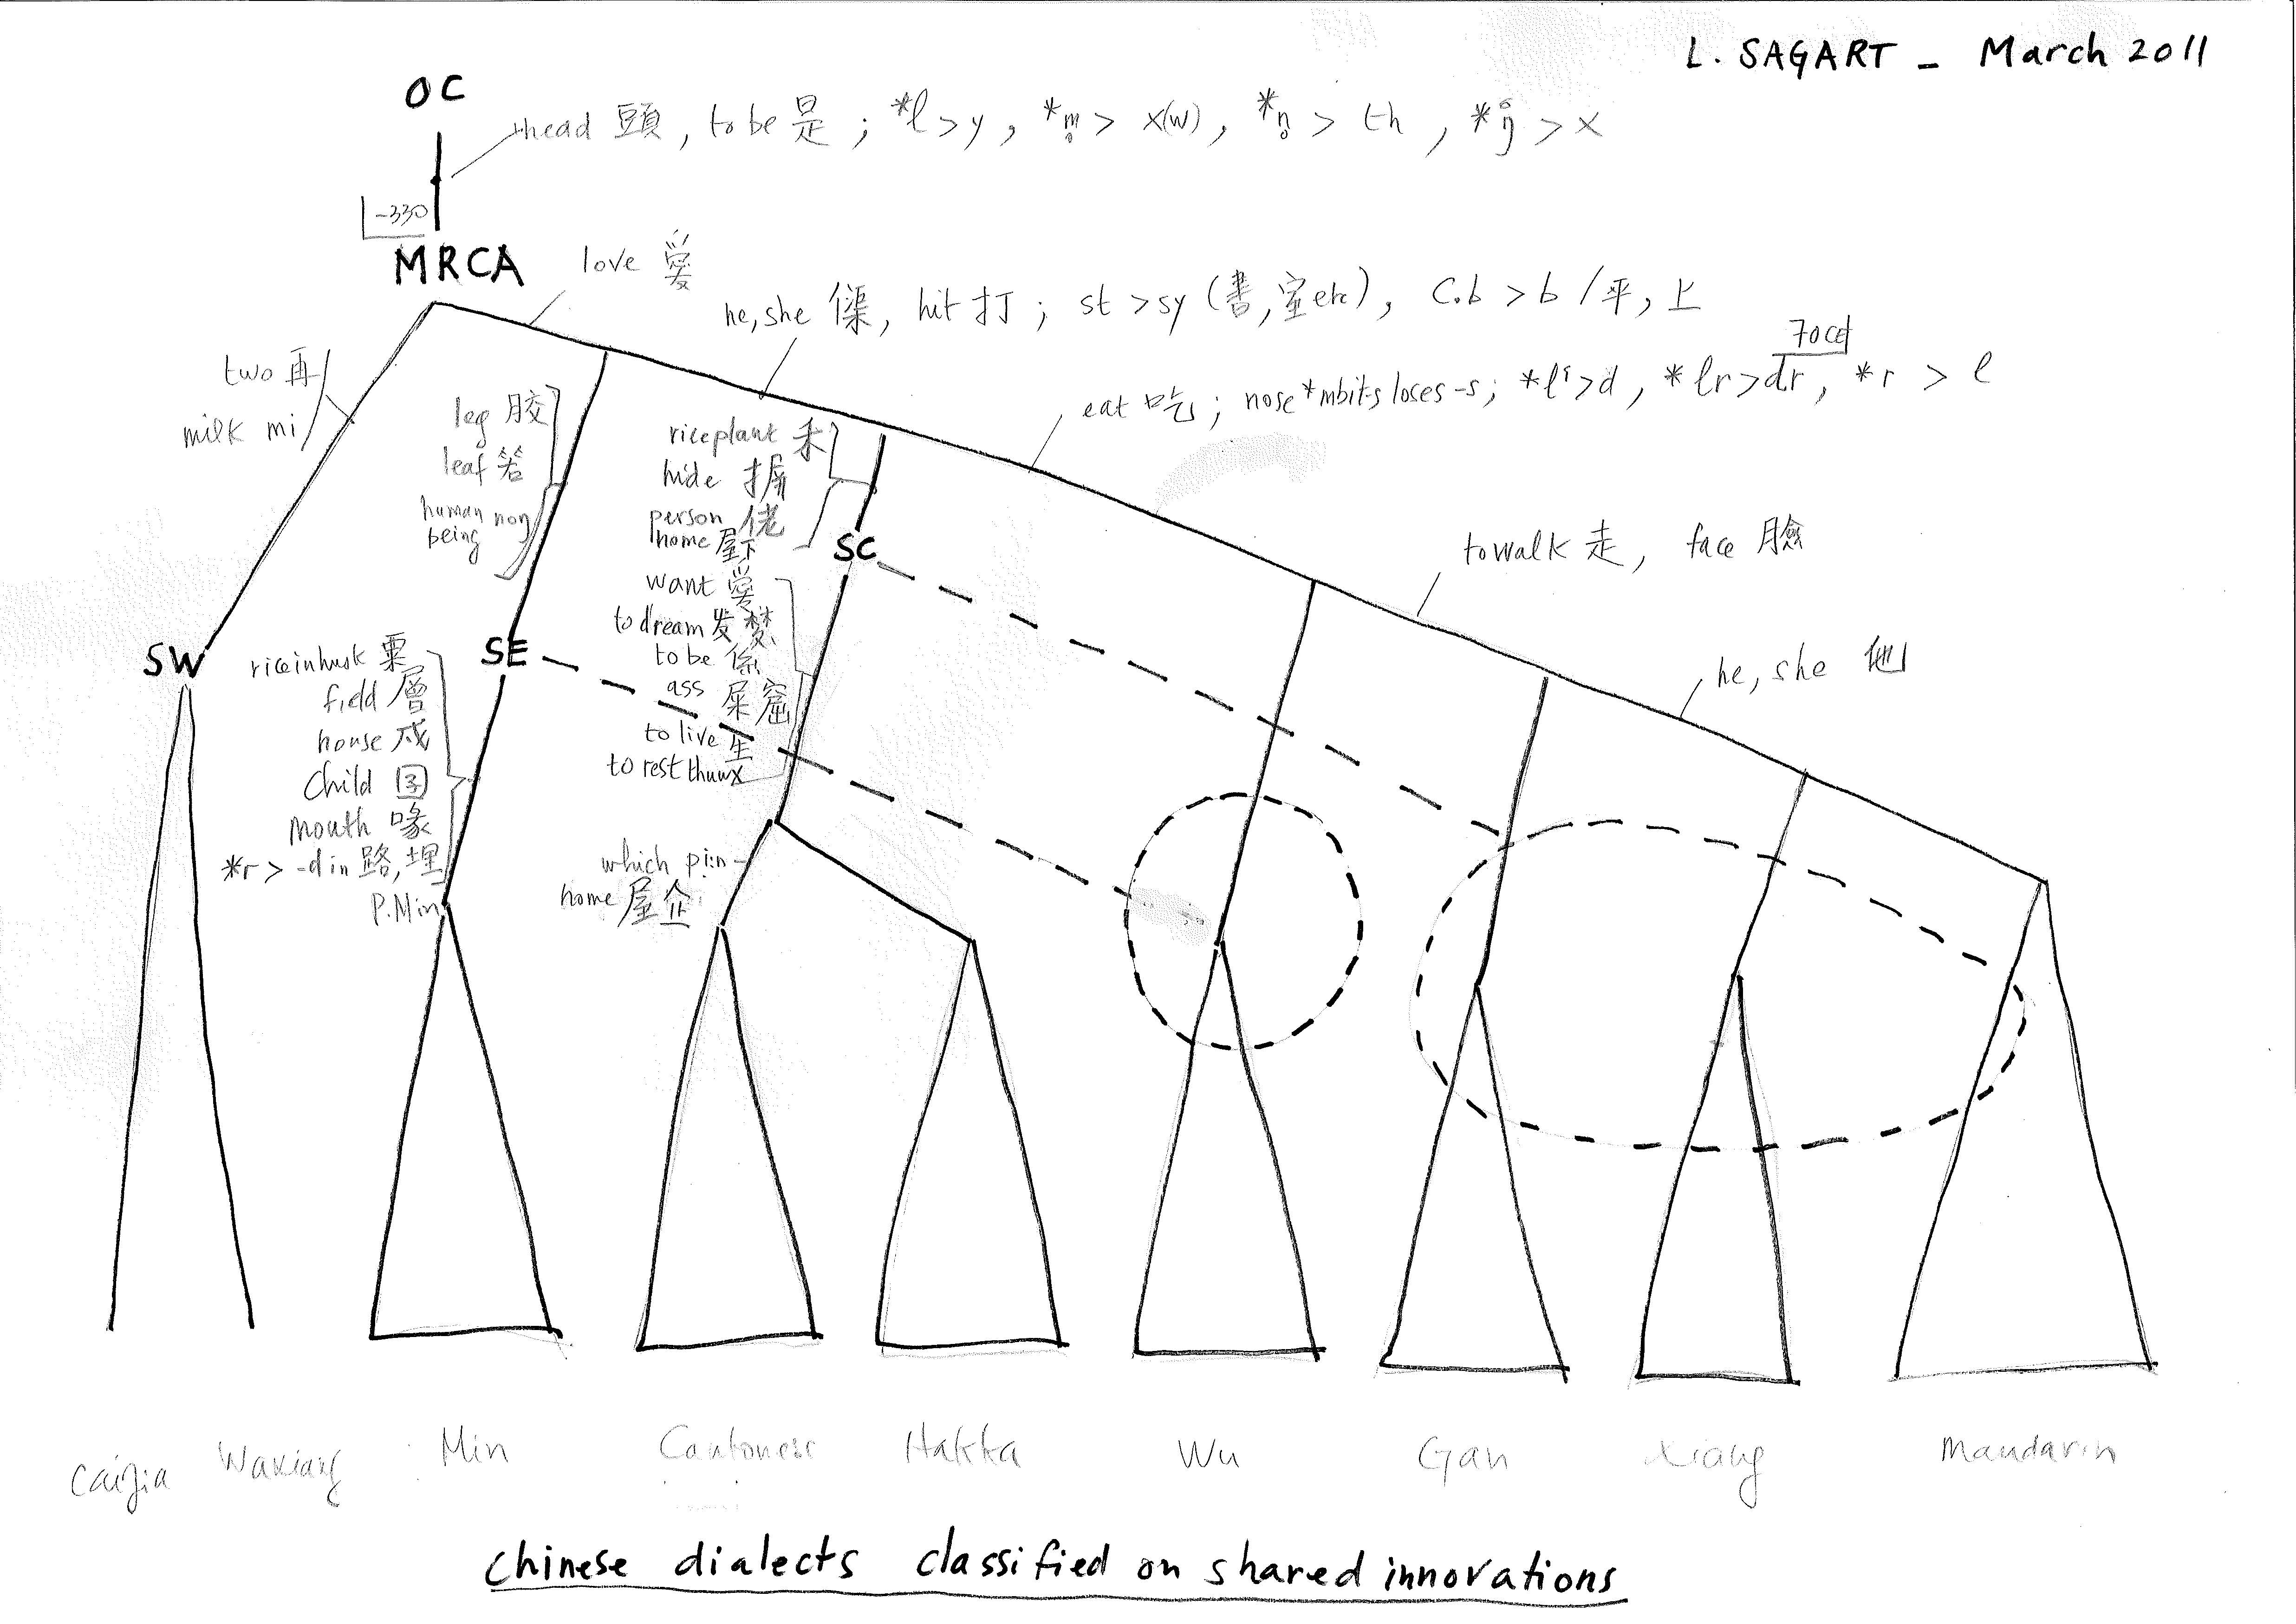
\includegraphics[scale=.3]{Figure/sagart}
\caption{L'arbre phylogénétique de \cite{sagart2011classifying}}
\label{fig:sagart_class}
\end{figure}

Néanmoins, il a donné les critères clairs pour décider les clades de l'arbre. Dans l'arbre établi par lui, c'est le Caijiahua (蔡家話) et le Waxianghua (瓦鄉話) qui constituent un clade qui se spépare d'abord de l'arbre. Ensuite le Min se sépare, suivi par le groupe constitué par le Yue et le Hakka. Le Wu, le Gan et le Xiang se séparent à tour de rôle, ce dernier constituant un clade avec le Mandarin. Bien que ce ne soit qu'une description préliminaire, il serait intéressant de comparer les résultats phylogénétiques obtenus avec les méthodes plus avancées avec celui de \textcite{sagart2011classifying}. %Puisque la stratification est une étape indispensable dans la collection des données, et que cette pratique n'a pas encore été effectuée d'une façon bien fine dans la phylogénie des langues sinitiques, ce mémoire prend comme problématique l'influence de l'exclusion des emprunts sur les résultats phylogénétiques des langues sinitiques.

Depuis que \textcite{Norman1979min} a proposé la question des couches dans les langues sinitiques, il y a déjà un certain nombre d'articles et d'ouvrages discutant cette question au niveau tant théorique que pratique. Il faut avouer que les études de ce sujet sont loin d'être complètes et profondes. La méthode de la stratification pour distinguer les couches est souvent liée au terme traditionnel ``wen-bai'' (文白) dans la dialectologie chinoise et se chevauche avec ce dernier par définition. Cela cause souvent des confusions dans les littératures. 

\textcite[341]{Norman2003kejia} propose l'importance de la distinction entre les formes orales et littéraires dans la classification des langues sinitiques. Mais il distingue ensuite une autre paire de notions : les ``formes familières'' et les ``formes populaires'' en indiquant que ce serait plutôt ces formes dernières qui comptent pour la classification. Peu importe, ce que \citeauthor{Norman2003kejia} veut dire est juste l'importance de la stratification dans la classification des langues sinitiques, et on compte surtout sur les couches héritées des langues afin d'obtenir les résultats pertinents. 
 
\textcite{wu2023annotating} établissent les arbres phylogénétiques des langues sinitiques avec des méthodes avancées et populaires. Ils proposent d'annoter les morphèmes saillants qui représentent l'histoire lexicale des langues pour améliorer les analyses phylogénétiques des langues parmi lesquelles existent beaucoup de stratégies morphologiques par la composition ou la dérivation avec un cas d'études des langues sinitiques, ce qui mérite d'être adopté comme une étape nécessaire de traitement des données des langues sinitiques. Ils essaient de marquer les emprunts dans leur base de données sans aborder l'influence de ces emprunts pour les résultats. Ainsi, ce mémoire a pour but de tester si l'exclusion des emprunts influencerait les résultats phylogénétiques des langues sinitiques et d'obtenir une impression préliminaire de ces résultats. On se sert de la même base de données déjà établie par \textcite{wu2023annotating} à partir des données collectées par \textcite{Liu2007hexinci}, dont les données doivent être corrigées et annotées au niveau des couches afin de passer à l'analyse phylogénétique. Pour ce faire, il faut d'abord établir les critères pour distinguer les couches des langues sinitiques. 

\chapter{Règles conventionnelles de transcription}
Voici ci-dessous quelques règles de transcription par convention : 

\stpc{c}\paragraph{(\arabic{c})}
Concernant les initiales du chinois moyen, on les divise en différents groupes selon la tradition par leurs points d'articulation et leurs modes d'articulation montrés dans la table \ref{tab:groupe_initiale}.

% Table generated by Excel2LaTeX from sheet '中古汉语'
\begin{table}[htbp]
  \centering
%\resizebox{\textwidth}{!}{
       \begin{tabular}{lcccc}
    \toprule
          & \multicolumn{2}{c}{Occlusive et sonante} & \multicolumn{2}{c}{Affriquée et fricative} \\
    \midrule
    Labial & \multicolumn{1}{c}{\cellcolor[rgb]{ .851,  .851,  .851}*p/pʰ/b/m- (幫組)} &       &       &  \\
    Labio-dental &       & \multicolumn{2}{c}{\cellcolor[rgb]{ .851,  .851,  .851}*f/fʰ/v/ɱ- (非組)} &  \\
    \midrule
    Alvéolaire & \multicolumn{1}{c}{\cellcolor[rgb]{ .851,  .851,  .851}*t/tʰ/d- (端組)} & \multicolumn{1}{c}{\cellcolor[rgb]{ .851,  .851,  .851}*n/ɳ/l- (泥組)} & \multicolumn{2}{c}{\cellcolor[rgb]{ .851,  .851,  .851}*ts/tsʰ/dz/s/z- (精組)} \\
    \midrule
    Rétroflexe & \multicolumn{1}{c}{\cellcolor[rgb]{ .851,  .851,  .851}*ʈ/ʈʰ/ɖ- (知組)} &       & \multicolumn{2}{c}{\cellcolor[rgb]{ .851,  .851,  .851}*tʂ/tʂʰ/dʐ/ʂ/ʐ- (莊組)} \\
    (Alvéolo-)palatal &       & \multicolumn{1}{c}{\cellcolor[rgb]{ .851,  .851,  .851}*ɲ- (日組)} & \multicolumn{2}{c}{\cellcolor[rgb]{ .851,  .851,  .851}*tɕ/tɕʰ/dʑ/ɕ/ʑ- (章組)} \\
    \midrule
    Vélaire & \multicolumn{2}{c}{\cellcolor[rgb]{ .851,  .851,  .851}*k/kʰ/g/ŋ- (見組)} &       & \multicolumn{1}{c}{\cellcolor[rgb]{ .851,  .851,  .851}*x/ɣ- (曉組)} \\
    Guttural & \multicolumn{2}{c}{\cellcolor[rgb]{ .851,  .851,  .851}*ʔ/ɣj/j- (影組)} &       &  \\
    \bottomrule
    \end{tabular}%}%
  \caption{Groupes d'initiales du chinois moyen}    
  \label{tab:groupe_initiale}%
\end{table}%
 
Ces initiales sont tellement regroupées sur la base de leurs comportements similaires dans l'évolution phonologique du chinois. Sauf indication contraire, on utilise le symbole de la première initiale dans chaque groupe pour le représenter. Il y a encore plusieurs points à noter : 

\begin{itemize}
\item{Le groupe *f- se sépare en fait du groupe *p- à l'époque postérieure du chinois moyen et se combine toujours avec une partie des rimes de la troisième division. On distingue ces deux groupes parce qu'elles se comportent souvent de différentes façons dans beaucoup de variantes.}

\item{Les initiales *j- et *ɣj- sont rattachées au groupe guttural *ʔ- selon la tradition pour gagner l'espace. En fait, ce serait plutôt la seule initiale *ʔ- qui est liée avec les initiales vélaires *k- et *x-.}

\item{Certains groupes peuvent encore être regroupés dans un super-groupe : le groupe labial *p- et le groupe labio-dental *f- constituent le super-groupe 幫系 ; les groupes alvéolaires *t-/*n-/*ts- constituent le super-groupe 端系 ; les groupes rétroflexes *ʈ-/*tʂ- et les groupes alvéolo-palataux *tɕ-/*ɲ- constituent le super-groupe 知系 ; les groupes vélaires *k-/*x- et le groupe guttural *ʔ- constituent le super-groupe 見系. Mais puisque les notations des groupes suffisent pour marquer l'origine des syllabes dans le chinois moyen, il suffit de juxtapose les symboles des groupes d'initiales pour marquer ces super-groupes, e.g. ``*k/x/ʔ-'' pour marquer le super-groupe 見系.}
\end{itemize}

\stpc{c}\paragraph{(\arabic{c})}
Pour faciliter les comparaisons entre les variantes, les tons sont souvent montrés sous forme de tonèmes (調類) mis à droite des syllabes, au lieu de leurs valeurs phonétiques. Les correspondances entre les symboles et les tonèmes sont donc représentées avec les lettres A/B/C/D et les chiffres 1/2 dans la table \ref{tab:Tonème}. 

% Table generated by Excel2LaTeX from sheet 'Tonème'
\begin{table}[htbp]
  \centering
%\resizebox{\textwidth}{!}{
    \begin{tabular}{lllll}
    \toprule
          & A (平-plat) & B (上-montant) & C (去-partant) & D (入-rentrant) \\
    \midrule
    \makecell{1 (陰-série \\supérieure)} & A1 (陰平) & B1 (陰上) & C1 (陰去) & D1 (陰入) \\
    \makecell{2 (陽-série \\inférieure)} & A2 (陽平) & B2 (陽上) & C2 (陽去) & D2 (陽入) \\
    \bottomrule
    \end{tabular}%}%
  \caption{Les symboles des tonèmes}
  \label{tab:Tonème}%
\end{table}%

Les nouveaux tonèmes séparés de ces tonèmes originaux sont marqués avec une apostrophe `` ' '' en haut à droite du symbole, comme dans le cas du tonème D1' du Yue de Guangzhou (cantonais). 

S'il n'y a plus de contraste entre les deux sous-tonèmes de la même paire, les chiffres 1/2 sont omis après les lettres A/B/C/D, comme dans le cas du tonème B dans beaucoup de variantes et le tonème D du mandarin de Nanjing.

%Pour les tonèmes confondus, ce nouveau tonème est montré par le symbole du tonème intégrant l'autre ou les autres tonèmes par référence à la tendance générale de la confusion des tonèmes dans la plupart des langues sinitiques. Par exemple, dans beaucoup de langues sinitiques, le tonème C1 sont normalement cencé couvrir les tonèmes originaux B2, C1 et C2 (des fois plus une partie du tonème D1 et D2). Il est dans certains cas difficile de déterminer le symbole du nouveau tonème inclusif faute d'indices, la solution dépend de la situation. Par exemple, dans le cas du mandarin de Nanjing, puisqu'il manque d'assez d'indices pour dire que le seul tonème rentrant soit D1 qui intègre D2 ou alors ce soit l'inverse, le symbole D qui neutralise cette distinction serait un meilleur choix.} %S'il n'y a pas assez d'indices pour déterminer le symbole du nouveau tonème inclusif, une solution possible est de mettre directement les valeurs en haut à droite des syllabes.

\stpc{c}\paragraph{(\arabic{c})}
Quand il n'y a pas de différence de l'initiale/de la rime/du tonème pour ces catégories comparées au sein d'une variante ou entre les variantes, celles-ci sont omises dans la transcription.

\stpc{c}\paragraph{(\arabic{c})}
Conventionnellement, on utilise le symbole [ʔ-] pour marquer l'initiale-zéro des langues sinitiques afin de faciliter l'analyse phonologique des structures syllabiques.

\stpc{c}\paragraph{(\arabic{c})}
Les symboles [ɿ/ʅ/ʮ/ʯ] sont utilisés par convention de la dialectologie chinoise pour signaler les voyelles dites ``apicale antérieure non-arrondie/postérieure non-arrondie/antérieure arrondie/postérieure arrondie'',qui se trouvent après les consonnes et donnent une impression acoustique de ces consonnes syllabiques, e.g. [sɿ] donne une impression acoustique de [s̩] non-arrondie. Selon 大百科词条(稿)舌尖元音\footnote{\url{http://www.360doc.com/content/20/0619/12/46996736_919350174.shtml}}, ce type de voyelles ``apicales'' sont fréquentes dans les langues sino-tibétaines et sont disctintes des voyelles palatales.

\stpc{c}\paragraph{(\arabic{c})}
Le symbole [ȵ] est utilisé par convention de la dialectologie chinoise pour signaler la nasale alvéolo-palatale, parallèle aux fricatives alvéolo-palatales [ɕ/ʑ] en API.

\stpc{c}\paragraph{(\arabic{c})}
Le symbole ``*'' avant les syllabes signifie la forme de reconstruction du chinois moyen selon \textcite{Baxter1992handbook}. Si la forme de reconstruction d'une syllabe n'existe pas, le statut phonologique de cette syllabe est donné par référence au \citetitle{CASSInsLin1981zibiao} et est converti à la forme marquée par le symbole ``**'' selon la reconstruction de \textcite{Baxter1992handbook}. Si jamais une syllabe ne se trouve nulle part dans ces deux ouvrages, la forme de reconstruction est laissée de côté provisoirement.

\chapter{Connotation du terme ``wen-bai''}\label{wenbai}
%Les \difwenbai sont assez fréquentes dans les langues sinitiques, vu le contact entre la variante locale et une autre variante externe (souvent la langue officielle ou la variante haute) dans l'histoire jusqu'ici. Généralement, la couche archaïque est considérée plus conservatrice et propre à cette variante même, alors que la couche récente se montre plus innovatrice et pourrait être attribuée à l'influence de la langue officielle ou à l'autre variante externe. Il est donc important de distinguer ces deux couches pendant l'annotation pour améliorer la crédibilité du résultat de la phylogénie. 
Le phénomène de ``wen-bai'' est assez fréquent dans les langues sinitiques, vu le contact entre la variante locale et une autre/d'autres variante(s) externe(s) (souvent la langue officielle ou la variante haute) dans l'histoire jusqu'ici. Beaucoup de savants/dialectologues chinois utilisent le terme ``文白異讀'' (lit. ``les prononciations littéraires et familières'') pour décrire le phénonème que sur une syllabe d'étymon existent plus de deux différentes prononciations employées dans différents contextes. Les prononciations littéraires (文讀) émergent sous le contact linguistique et sont employées dans la lecture alors que les prononciations familières (白讀) sont indigènes et sont employées dans l'oral. 

\section{Insuffisances du terme ``wen-bai''}\label{cntn_wenbai}
Cette notion se chevauche partiellement avec la notion des ``\difwenbai'' qu'on utilise dans ce mémoire. Malheureusement, le terme ``wen-bai'' peut poser la question pour les raisons suivantes :

D'abord, la frontière entre les ``wen-bai'' peut des fois être assez floue :  l'emploi des prononciations littéraires/familières dans la lecture/l'oral n'est pas absolu. %Effectivement, il vaut mieux reformuler le fait comme ``les prononciations littéraires/familières sont respectivement employées \textbf{initialement} dans la lecture/l'oral, sans exclure leur emploi dans l'oral/la lecture''. 
Les prononciations littéraires peuvent aussi exister dans l'oral, e.g. si l'on parle d'un concept moderne ; les prononciations familières peuvent aussi exister dans la lecture, e.g. quand une syllabe n'a que la prononciation appartenant à la couche archaïque qui n'a pas encore été remplacée par la prononciation de la couche récente\footnote{Par exemple, la syllabe 豇 (\bolang 豆, ``Vigna unguiculata'') (*kæwŋ) n'a souvent qu'une prononciation avec l'initiale [k-] appartenant à la couche archaïque dans beaucoup de variantes Wu du Nord, tant dans la lecture que dans l'oral. Le degré conservateur de la prononciation d'une syllabe peut dépendre des variantes, des locuteurs, du lexique, etc.}.

Il s'ensuit un problème qui peut souvent être troublant: l'idnetification des prononciations comme ``littéraire'' ou ``familière'' peut être une pratique assez subjective, ce qui cause la possibilité de la confusion entre les prononciations appartenant respectivement à la couche archaïque et à la couche récente. Pour la plupart du temps, les prononciations familières sont censées être conservatrices et les prononciations littéraires sont censées être innovatrices. Mais pour mieux distinguer les prononciations des \difwenbai, les critères les plus important sont toujours \textbf{phonétiques} au lieu des contextes où elles sont employées. Sous le terme ``wen-bai'', il arrive que certains savants identifient certaines prononciations \textbf{``conservatrices''} comme \textbf{``littéraires''}, alors que les prononciations \textbf{``innovatrices''} comme \textbf{``familières''}, ce qui risque d'induire en erreur ceux qui profite directement de ces données pour l'identification des \difwenbai. 

Enfin, le terme ``wen-bai'' englobe non seulement le cas des \difwenbai, mais aussi d'autres cas où les différentes prononciations d'une syllabe devraient être attribuées à d'autres motivations. Ce point sera illustré plus en détail ci-dessous.

\section{Phénomènes apparemment similaires à ``wen-bai''}\label{phnmn_idtf}
Lors de l'identification des \difwenbai sur la base de la littérature sur le terme ``wen-bai'', il faut d'abord identifier au moins cinq types de phénomènes qui sont apparemment similaires au phénomène de ``wen-bai'', mais sont différents de celui-ci à différents degrés. \textcite{Shen1988shanghai} discute de ce sujet et propose beaucoup d'exemples de ce type du Wu de Shanghai. On se réfère à cet article et profite aussi d'autres variantes du Wu pour aborder ces phénomènes ci-dessous en rajoutant quelques exemples personnels.

\subsection{Alternance morphologique (\cite[134]{Shen1988shanghai})}\label{phenom1}
Cela veut dire que sur une syllabe existent apparemment différentes prononciations, mais ces prononciations proviennent en fait de l'alternance morphologique entre différents allomorphes partageant la même écriture/étymologie dans le chinois moyen. 

\stpc{c}\paragraph{(\arabic{c})}
Un exemple intéressant consiste à la syllabe 伏 dans les Wu de Suzhou, où il existe apparemment trois prononciations sur la même syllabe 伏 : 

\begin{itemize}
\item{[buC2], ``couver'' (\cite[27]{Ye1993Suzhou}) ;}

\item{[boA2], ``s'appuyer (sur la table)'' (\cite[277]{Ye1993Suzhou})\footnote{(\cite[277]{Ye1993Suzhou}) représente cette syllabe par la forme ``爬'' dans la structure ``合爬''[ɦəʔ-boA2] qui signifie ``s'appuyer (sur la table)''. Mais dans le Wu de Shanghai, la syllabe [boʔ] peut toute seule exprimer ce sens (\cite[381]{Xu1997shanghai}) ; en même temps, il y a aussi une autre structure ``合撲''[ɦəʔ-pʰoʔ] avec le même sens (\cite[348]{Xu1997shanghai}). Alors que dans le Wu de Jiangyin (Shengang), la langue maternelle de l'auteur, cette structure se prononce bien comme [ɦəʔ-boʔ]. Donc il est probable que ces différentes prononciations [boA2/pʰoʔ] proviennent toutes de la prononciation [boʔ], càd. la syllabe 伏.} ;}

\item{[voʔD2], ``se posterner ; canicule'' (\cite[296]{Ye1993Suzhou}).}
\end{itemize}

Cependant, la prononciation [buC2] provient de l'allomorphe 伏1 (*bjuwH) et les deux prononciations [boʔD2] et [voʔD2] proviennent de l'allomorphe 伏2 (*bjuwk). Mais c'est plutôt les prononciations [buC2] et [boʔD2] qui appartiennent à la même couche archaïque, et la prononciation [voʔD2] appartient à la couche récente. On a donc un mélange de deux phénomènes : l'alternance morphologique d'une part, et la différence des \difwenbai de l'autre. \illustre \ref{tab:exemple_morpho1}.

% Table generated by Excel2LaTeX from sheet '排除'
\begin{table}[htbp]
  \centering
%\resizebox{\textwidth}{!}{
    \begin{tabular}{lllll}
    \toprule
    Critère & Syllabe & Chinois moyen  & Couche archaïque & Couche récente \\
    \midrule
    \multirow{2}[2]{*}{Rime} & 伏1    & *bjuwH & [buC2] &  \\
          & 伏2    & *bjuwk & [boA2] (< [boʔD2]) & [voʔD2] \\
    \bottomrule
    \end{tabular}%}%
  \caption{Prononciations de la syllabe 伏 du Wu de Suzhou}
  \label{tab:exemple_morpho1}%
\end{table}%

\stpc{c}\paragraph{(\arabic{c})}
Un autre exemple similaire consiste à la syllabe 射 du Wu de Suzhou (\cite[26]{Ye1988suzhou}). Il y a trois rimes sur cette syllabe : [-o], [-ʏ] et [-oʔ]. Les rimes [-oC2] et [-oʔD2] sont propres au Wu de Suzhou mais proviennent de différents allomorphes : la rime [-oC2] provient de 射1 (ʑæH) et la rime [-oʔD2] semble provenir de 射2 (*ʑek)\footnote{C.f. les rimes des autres syllabes partageant le même groupe de rimes dans la même contexte : 隻 (*tɕek) [tsɑʔ], 尺 (*tɕʰek) [tsʰɑʔ] et 石 (*dʑek) [fam. zɑʔ/lit. zəʔ]. La rime [-oʔ] de 射2 (*ʑek) semble appartenir à l'autre couche que les syllabes précédentes, mais cela n'empêche pas qu'elle appartient à l'autre allomorphe que 射1.}. En ce qui concerne la troisième rime [-ʏC2], il faut regarder trois autres syllabes 者 (tɕæX) 奢 (ɕæ) 社 (dʑæX) du même groupe de rimes. Toutes les quatre syllabes appartiennent à celles \termyyx{à initiales *tɕ- et à la rime *-jæ (章組假攝三等字)}. Cette série de syllabes ont normalement la rime [-o] appartenant à la couche archaïque dans le Wu de Suzhou. Mais \textcite[161, 162, 167]{Ye1988suzhou_fangyanzhi} et \textcite[5, 10, 14]{Shi2019she_suzhou} mentionnent qu'il existe d'autres rimes [-e] ou [-ʏ] sur (certaines de) ces quatre syllabes. \illustre \ref{tab:exemple_jia3_suzhou}. Les pages de référence sont jointes après les rimes. Notez que les données de \textcite[5, 10, 14]{Shi2019she_suzhou} sont en fait reconstruites sur la base de deux matériaux du Wu de Suzhou publiés en 1892 et 1935 et sont donc plus anciennes que celles de \textcite[161, 162, 167]{Ye1988suzhou_fangyanzhi}, qui n'a pas pourtant mentionné les informations concrètes des informateurs.

% Table generated by Excel2LaTeX from sheet '苏州'
\begin{table}[htbp]
  \centering
%\resizebox{\textwidth}{!}{
    \begin{tabular}{lllll}
    \toprule
          & 者 (*tɕæX) & 奢 (*ɕæ) & 射 (*ʑæH) & 社 (*dʑæX) \\
    \midrule
    \textcite{Shi2019she_suzhou}     & [-ʏ] (5) & [-e] (10) & [-ʏ] (14) & [-ʏ] (14) \\
    \textcite{Ye1988suzhou_fangyanzhi}     & [-e/-ʏ] (161/167) & [-ʏ] (167) & [-o] (162) & [-o] (162) \\
    \bottomrule
    \end{tabular}%}%
  \caption{Rimes sur les syllabes 者奢射社 du Wu de Suzhou}
  \label{tab:exemple_jia3_suzhou}%
\end{table}%

\textcite[14]{Shi2019she_suzhou} remarque que les syllabes 射社 avaient la rime [-ʏ] mais ont aujourd'hui de nouveau la rime régulière [-o], alors que les syllabes 者奢 gardent encore les rimes [-e/-ʏ]. Il est probable que les rimes [-e] et [-ʏ] appartiennent à différentes couches récentes sous l'influence du mandarin. 

Ainsi, parmi les trois rimes [-oC2/-oʔD2/-ʏC2], les rimes [-oC2] et [-ʏC2] proviennent de l'allomorphe 射1, et la rime [-oʔD2] provient de l'autre allomorphe 射2. Mais c'est plutôt les rimes [-ʏC2] et [-oʔD2] qui appartiennent à la couche récente, et la rime [-oC2] qui appartient à la couche archaïque.  \illustre \ref{tab:exemple_morpho2}.

% Table generated by Excel2LaTeX from sheet '形态交替'
\begin{table}[htbp]
  \centering
%\resizebox{\textwidth}{!}{
    \begin{tabular}{lllrl}
    \toprule
    Critère & Syllabe & Chinois moyen  & \multicolumn{1}{l}{Couche archaïque} & Couche récente \\
    \midrule
    \multirow{2}[2]{*}{Rime} & 射1    & *ʑjæH & \multicolumn{1}{l}{[-oC2]} & [-ʏC2] (a) \\
          & 射2    & *ʑek  &       & [-oʔD2] (b) \\
    \bottomrule
    \end{tabular}%}%
  \caption{Prononciations de la syllabe 射 du Wu de Suzhou}
  \label{tab:exemple_morpho2}%
\end{table}%

Dans un sens strict, puisque les rimes [-ʏC2] et [-oʔD2] appartiennent toutes à la couche récente (probablement à différentes couches), et que la rime [-ʏC2] ne s'utilise plus aujourd'hui, le lien morphologique entre ces deux rime n'est pas assez clair et typique. Mais comme le cas de 伏, le cas de 射 révèle aussi la complication résultant de différents allomorphes dans l'histoire quand on cherche à identifier les \difwenbai.

Les deux exemples précédents concernent tous l'alternance morphologique entre différents allomorphes partageant la même écriture/étymologie attestées dans le chinois moyen. Cette alternance morphologique peut aussi ne pas être attestée dans le chinois moyen, probablement parce qu'elle s'est produite plus tard que l'époque de Qieyun, ce qui est exemplifié par l'alternance entre les initiales sonores et sourdes sur certaines syllabes dans les Wu de Shanghai (\cite[132--133]{Shen1988shanghai}) et Wenzhou (\cite[107]{Zhengzhang2008wenzhou}). \illustre \ref{tab:exemple_morpho3}.

% Table generated by Excel2LaTeX from sheet '形态交替'
\begin{table}[htbp]
  \centering
%\resizebox{\textwidth}{!}{
    \begin{tabular}{lllll}
    \toprule
    Wu    & Syllabe & Chinois moyen  & Initiale I & Initiale II \\
    \midrule
    \multirow{2}[2]{*}{Shanghai} & 攪     & *kæwX & [k-C1] & [g-C2]     \\
          & 擱     & *kak  & [k-D1] & [g-D2] \\
    \midrule
    \multirow{2}[2]{*}{Wenzhou} & 爭     & *tʂɛŋ & [ts-A1] & [dz-A2/C2] \\
          & 下     & *ɣæX/*ɣæH & [ʔ-B1/C1] & [ɦ-B2/C2] \\
    \bottomrule
    \end{tabular}%}%
  \caption{Prononciation des syllabes 攪擱爭下 des Wu de Shanghai et de Wenzhou}
  \label{tab:exemple_morpho3}%
\end{table}%

\subsection{Etymologie opaque (\cite[138]{Shen1988shanghai})}\label{phenom2}
Cela veut dire que les apparemment différentes prononciations sur une syllabe appartiennent en fait à différents étymons sauf qu'il est difficile de déterminer l'étymologie. Les prononciations non étymologiques ressemblent à la notion ``kun-yomi'' (訓読み) du japonais.

Cela peut être exemplifié par les syllabes 左 et 蘿 dans les Wu de Suzhou (\cite[26]{Ye1988suzhou}) et Shanghai (\cite[133, 138]{Shen1988shanghai}). L'opinion que la prononciation [tsi] qui signifie ``gauche'' provienne bien de la syllabe 左 qui se prononce normalement comme [tsəu] (en Wu de Suzhou)/[tsu] (en Wu de Shanghai) n'est pas toujours convaincante, et ce morphème est souvent représenté par l'écriture 濟 ou 借 par certains savants\footnote{\textcite[291--292]{Wang2003benzi} pense que l'étymologie de la prononciation [tsi] est bien la syllabe 左 et qu'elle appartient à la couche de Qieyun. \textcite{Zheng2009guo_wu} pense que la prononciation [tsi] provient de la syllabe 左 et appartient à la couche antérieure à Qieyun. \textcite{Wang2015zuo_wu} conteste cette opinion par manque du parallélisme avec cette syllabe, et pensent que le vrai étymon serait 濟 ou 借.}. 

C'est le même cas avec la syllabe [læ] (en Wu de Suzhou)/[lɔ] (en Wu de Shanghai) qui est employée dans le mot [læ-boʔ/lɔ-boʔ] pour signifier ``radis'' et diffère de la prononciation de la syllabe 蘿[ləu] (en Wu de Suzhou). Certains savants représentent donc ``radis'' par l'écriture 老蔔 au lieu de 蘿蔔, mais ce n'est pas décisif. \illustre \ref{tab:exemple_etymon}.

% Table generated by Excel2LaTeX from sheet '形态交替'
\begin{table}[htbp]
  \centering
%\resizebox{\textwidth}{!}{
    \begin{tabular}{lllll}
    \toprule
    Critère & Syllabe & Chinois moyen  & Suzhou & Shanghai \\
    \midrule
    \multirow{2}[2]{*}{Rime} & 蘿 & *la   & [-əu] & [-u] \\
          & 老(?)(\bolang 蔔) & *lawX & [-æ]  & [-ɔ] \\
    \midrule
    \multirow{2}[2]{*}{Rime}
          & 左 & *tsaX & [-əu] & [-u] \\
          & 濟(?)/借(?)(\bolang 手) & *tsejH/*tsjæH & [-i]  & [-i] \\
    \bottomrule
    \end{tabular}%}%
  \caption{Prononciation des syllabes 蘿左 des Wu de Suzhou et Shanghai}
  \label{tab:exemple_etymon}%
\end{table}%

\subsection{Changement phonétique discursif (\cite[134--136]{Shen1988shanghai})}\label{phenom3}
Cela veut dire que les différentes prononciations sur une syllabe sont attribuées au changement phonétique discursif, comme l'assimilation, la dissimilation, la lénition, etc.

\stpc{c}\paragraph{(\arabic{c})}
Un phénomène typique est la perte des médianes, e.g. la syllabe 别[bəʔ] (au lieu de [bieʔ]) dans le mot 別人 (``d'autres personnes''), la syllabe 快[kʰa] (au lieu de [kʰua]) dans le mot 快活 (``agréable'') et la syllabe 還 qui se prononce comme [uɛA1<ɦuɛC2<ɛA1<ɦɛC2] selon la fréquence d'usage quand elle signifie ``encore'' dans les mots comme 還有 et 還要 dans le Wu de Shanghai (\cite[134]{Shen1988shanghai}). \illustre \ref{tab:exemple_mediane}.

% Table generated by Excel2LaTeX from sheet '形态交替'
\begin{table}[htbp]
  \centering
%\resizebox{\textwidth}{!}{
    \begin{tabular}{lllll}
    \toprule
    Critère & Syllabe & Chinois moyen  & Rime I & Rime II \\
    \midrule
    \multirow{3}[2]{*}{Rime} & 别 & *pjet & [-əʔ] (\bolang 人) & [-iəʔ] \\
          & 快 & *kʰwæjH & [-a] (\bolang 活)  & [-ua] \\    
          & 還 & *ɣwæn & [-ɛ] (\bolang 有)  & [-uɛ] \\
    \bottomrule
    \end{tabular}%}%
  \caption{Prononciation des syllabes 别快還 du Wu de Shanghai}
  \label{tab:exemple_mediane}%
\end{table}%

Mais on pense que les motivations des changements phonétiques pour les syllabes 別快 d'une part et la syllabe 還 de l'autre sont différentes. Pour les syllabes 別 et 快, il est possible que la motivation de la perte de leurs médianes est la dissimilation sous l'inifluence de la voyelle [i] et [u] dans les syllabes suivantes 人 et 活 : 

(1) 別人[biəʔ-ȵin] > [bəʔ-ȵin]

(2) 快活[kʰwa-ɦuəʔ] > [kʰa-ɦuəʔ]

Alors que pour la syllabe 還, la motivation de la perte de sa médiane serait plutôt la lénition à force d'usage comme un mot grammatical. Pour la discussion plus en détail du changement phonétique exceptionnel des mots grammaticaux, voir la partie \ref{excep_mot_gram}. Cela permet d'expliquer pourquoi les prononciations sans médianes des syllabes 別 et 快 ne s'utilisent que dans les mots 別人 et 快活, alors que la prononciation sans médiane de la syllabe 還 s'utilise d'une façon assez fréquente. Effectivement, \textcite[134]{Shen1988shanghai} mentionne aussi la syllabe 又, un autre mot grammatical dans le Wu de Shanghai, qui a une prononciation régulière [ɦiɤ], une prononciation dans la lecture [iɤ] et une troisième prononciation irrégulière [ɦi]. Celle-ci devrait aussi être le résultat de la lénition qui ne donne pas forcément la perte de la médiane.

\stpc{c}\paragraph{(\arabic{c})}
Un autre exemple consiste aux syllabes 鯽鯖 dans les Wu de Suzhou (\cite[26]{Ye1988suzhou}) et Shanghai (\cite[134--135]{Shen1988shanghai}). \textcite[134--135]{Shen1988shanghai} décrit le processus de la formation de leurs différentes prononciations : ces deux syllabes qui se prononcent respectivement comme [tsiəʔ/tsʰin] initialement sont souvent suivies de l'autre syllabe 魚 qui se prononce comme [ŋ̩]. Dans le discours courant, la syllabe suivante [ŋ̩] influence les syllabes précédentes en les changeant en [tsin/tsʰi] respectivement : 

(1) 鯽魚[tsiəʔ-ŋ̩] > [tsin-ŋ̩] (assimilation) ;  

(2) 鯖魚[tsʰin-ŋ̩] > [tsʰi-ŋ̩] (dissimilation). 

\noindent Ces deux prononciations [tsin/tsʰi] sont donc les résultats de la prononciation consécutive. \illustre \ref{tab:exemple_interne}.

% Table generated by Excel2LaTeX from sheet '形态交替'
\begin{table}[htbp]
  \centering
%\resizebox{\textwidth}{!}{
    \begin{tabular}{lllll}
    \toprule
    Critère & Syllabe & Chinois moyen  & Rime I & Rime II \\
    \midrule
    \multirow{2}[2]{*}{Rime} & 鯽     & *tsik & [-inC1] & [-iəʔD1] \\
          & 鯖     & *tsʰeŋ & [-i] & [-in] \\
    \bottomrule
    \end{tabular}%}%
  \caption{Prononciation des syllabes 鯽鯖 des Wu de Shanghai}
  \label{tab:exemple_interne}%
\end{table}%

\subsection{Confusion des homophones (\cite[135]{Shen1988shanghai})}\label{phenom4}
Cela veut dire que les différentes prononciations sur une syllabe sont motivées par la possibilité de ne pas causer des confusions des homophones, ce qui est exemplifié par les syllabes 枇 v.s. 琵 (*bjij) et 葡 v.s. 蒲 (*bu) qui partagent le même statut phonologique du chinois moyen dans les Wu de Suzhou (\cite[26]{Ye1988suzhou}) et Shanghai (\cite[135]{Shen1988shanghai}). \textcite[135]{Shen1988shanghai} explique la motivation de la formation de différentes prononciations sur ces deux syllabes : la syllabe 枇 porte la rime [-iəʔD2] au lieu de la rime régulière [-iA2] dans le mot 枇杷 afin que les locuteurs ne confondent pas les mots 枇杷[bieʔ-bo](``nèfle du Japon'') v.s. 琵琶[bi-bo] (``pipa (instrument)'') ; la syllabe 葡 porte la rime [-əʔD2] au lieu de la rime régulière [-uA2] dans le mot 葡萄 afin que les locuteurs ne confondent pas les mots 葡萄[bəʔ-dɔ] (``raisin'') v.s. 蒲桃[bu-dɔ] (``noix''). Mais dans d'autres mots composés de ces deux syllabes, e.g. 葡萄酒 (``vin''), 葡萄牙 (le Portugal), etc. ces deux syllabes se prononcent comme [bi/bu], les prononciations régulières\footnote{\textcite[135]{Shen1988shanghai} n'a pas proposé d'exemple de la syllabe 枇. Mais selon l'enquête de l'auteur, dans le Wu de Jiangyin (Shengang), il existe de similaires phénomènes sur les syllabes 枇 et 葡 qui se prononcent comme [biəʔ/bu] dans les mots 枇杷 et 葡萄. Et la syllabe 枇 dans le mot 枇杷膏 (``un sirop contre la toux'') se prononce comme [bi], la prononciation régulière.}, probablement parce qu'il n'est plus possible de confondre ces mots avec d'autres. \illustre \ref{tab:exemple_homo}.

% Table generated by Excel2LaTeX from sheet '形态交替'
\begin{table}[htbp]
  \centering
%\resizebox{\textwidth}{!}{
    \begin{tabular}{lllll}
    \toprule
    Critère & Syllabe & Chinois moyen  & Rime I & Rime II \\
    \midrule
    \multirow{2}[2]{*}{Rime} & 枇 & *bjij  & [-iəʔD2] (\bolang 杷) & [-iA2] (\bolang 杷膏) \\
          & 葡 & *bu   & [-əʔD2] (\bolang 萄) & [-uA2] (\bolang 萄酒) \\
    \bottomrule
    \end{tabular}%}%
  \caption{Prononciation des syllabes 枇葡 du Wu de Shanghai}
  \label{tab:exemple_homo}%
\end{table}%

\subsection{Influence de l'écriture (\cite[138]{Shen1988shanghai})}\label{phenom5}
Cela veut dire que l'écriture peut des fois induire en erreur les locuteurs et causer des prononciations erronées. Ces prononciations erronées appartiennent normalement à la couche récente, mais peuvent parfois passer pour celles appartenant à la couche archaïque. 

\stpc{c}\paragraph{(\arabic{c})}
Par exemple, \textcite[21]{Ye1988suzhou} mentionne que la syllabe 莢 (*kep) a deux prononciations [kaʔ] et [tɕiaʔ] et pense qu'elles appartiennent respectivement aux \difwenbai. Mais \textcite[184]{Ye1988suzhou_fangyanzhi} n'enregistre qu'une prononciation [tɕiəʔ] (Il l'a mal écrit comme 筴). Evidemment, les deux premières prononciations sont erronées sous l'influence de l'élément phonétique 夾 (*kɛp) qui par contre a pour couche archaïque la prononciation [kaʔ] et pour couche récente la prononciation [tɕiaʔ] (\cite[21]{Ye1988suzhou}). Si l'on n'identifie pas par avance les deux premières prononciations erronées, elles risqueront de passer pour celles appartenant respectivement aux \difwenbai.

\stpc{c}\paragraph{(\arabic{c})}
Un autre exemple consiste à la syllabe 峽 (*ɣɛp) dans les Wu de Suzhou et Wenzhou. Dans ces deux variantes, cette syllabe a une prononciation correcte [ɦiaʔ] (Suzhou)\footnote{\textcite{Ye1988suzhou_fangyanzhi} n'a pas mentionné cette prononciation, mais cette prononciation existe dans le Wu de Jiangyin (Shengang) selon l'enquête de l'auteur.}/[ɡaD2] (Wenzhou) et une prononciation erronée [tɕiaʔ] (Suzhou)/[kaD1] (Wenzhou) sous l'influence de 夾 encore. Ce cas ne pose pas la question comme le cas de 莢 parce que les prononciations erronées n'ont pas de possibilité d'être considérées comme appartenant à la couche archaïque. \illustre \ref{tab:exemple_ecriture}.

% Table generated by Excel2LaTeX from sheet '形态交替'
\begin{table}[htbp]
  \centering
%\resizebox{\textwidth}{!}{
    \begin{tabular}{lllll}
    \toprule
    Wu    & Syllabe & Chinois moyen  & \makecell[l]{Prononciation\\ correcte} & \makecell[l]{Prononciation\\ erronée} \\
    \midrule
    \multirow{2}[2]{*}{Suzhou} & 莢     & *kep  & [tɕiəʔ] & [kaʔ/tɕiaʔ] \\
          & 峽     & *ɣɛp  & [ɦiaʔ] & [tɕiaʔ] \\
    \midrule
    Wenzhou & 峽     & *ɣɛp  & [gaD2] & [kaD1] \\
    \bottomrule
    \end{tabular}%}%
  \caption{Prononciations des syllabes 莢峽 des Wu de Suzhou et Wenzhou}
  \label{tab:exemple_ecriture}%
\end{table}%

Pour résumer, il y a au moins cinq types de phénomènes apparemment similaire au phénomène de ``wen-bai'' qui doivent bien être identifiés avant d'identifier les \difwenbai : \textbf{(1) alternance morphologique} (\ref{phenom1}) ; \textbf{(2) étymologie opaque} (\ref{phenom2}) ; \textbf{(3) changement phonétique discursif} (\ref{phenom3}) ; \textbf{(4) confusion des homophones} (\ref{phenom4}) ; \textbf{(5) influence de l'écriture} (\ref{phenom5}). Il est remarquable que puisque ces phénomènes ont souvent peu à avoir avec le changement phonétique conditionné, beaucoup de syllabes de ces types sont distribuées d'une façon \textbf{sporadique}.  Certains de ces phénomènes peuvent se chevaucher partiellement avec le phénomène de ``wen-bai'' : 

Pour (1) et (2), il est quand-même possible que certaines prononciations concernées appartiennent à différentes couches, comme les cas de 伏 et 射, parce que même si deux prononciations proviennent de différents morphèmes ou allomorphes, elles peuvent encore appartenir à différentes couches. Pour (3) et (4), ce sont plutôt des cas dûs à la motivation interne du système et peuvent donc être directement exclus de ``wen-bai''. Pour (5), la situation est moins problématique que les cas précédents, parce que les prononciations correctes et les prononciations erronées appartiennent respectivement aux \difwenbai, même si ces dernières sont erronées. Mais il faut bien identifier les prononciations erronées et les rattacher à la couche récente pour éviter qu'elles ne troublent l'analyse, comme dans le cas de 莢.

En tous cas, l'idée ici est de mieux déterminer la connotation du terme ``wen-bai'' en distinguant le phénomène de ``wen-bai'' et les autres phénomènes apparemment similaires afin de pouvoir  obtenir des données pertinentes servant de base pour la stratification dont on parlera plus loin. Malheureusement il sera au-delà de la portée de ce mémoire d'élaborer des critères détaillés pour parfaitement identifier ces phénomènes. Il faut donc être assez prudent lors de leur identification. %Dans le texte suivant, on se contente d'exclure ces phénomènes non pertinents en n'indiquant que les cinq types qu'appartiennent ceux-ci.

Ainsi, le terme ``wen-bai'' dans la dialectologie chinoise n'est pas assez satisfaisant pour la description des \difwenbai, parce qu'il distingue deux types de prononciations selon le contexte d'emploi qui est un critère assez flou et subjectif, et qu'il englobe beaucoup de phénomènes de différentes natures qui peuvent compliquer l'identification des couches. Il vaux mieux utiliser la notion des \textbf{prononciations ``archaïque/conservatrice et récente/innovatrice''} et la notion des \textbf{``\difwenbai ''} qu'on va utiliser dans ce mémoire. 

\section{Insuffisance de la dichotomie ``wen-bai'' et la méthode de la stratification}
Il faut aussi noter la limite de la dichonomie entre les \difwenbai : 

\stpc{c}\paragraph{(\arabic{c})}
D'une part, pour chaque syllabe, l'identification d'une prononciation donnée comme appartenant à la couche archaïque ou récente est toujours \textbf{ponctuelle}. Par exemple, dans le Wu de Suzhou, si l'on tient en compte la syllabe 多, la rime [-ɑ] appartient à la couche archaïque, alors que la rime [-əu] appartient à la couche récente, parce que la rime [-ɑ] est plus proche de la rime équivalente du chinois moyen *-a, la source interne, et cette syllabe à cette rime ne s'utilise que dans très peu de mots aujourd'hui ; par contre, dans le cas de la syllabe 大, la rime [-əu] appartient à la couche archaïque et la rime [-ɑ] appartient à la couche récente, parce que la rime [-ɑ] est plus proche de la rime équivalente du mandarin, la source externe, et cette syllabe à cette rime s'utilise normalement dans les mots modernes ou littéraires, comme 大學 (``université''), 大衆 (``masse''), etc. L'une des rimes [-əu] et [-ɑ] appartient donc à la couche archaïque, l'autre à la couche récente et vice versa, en fonction des syllabes. \illustre \ref{tab:exemple_wenbai_Suzhou}.\label{sec:exemple_duo_da_suzhou}

% Table generated by Excel2LaTeX from sheet '蘇州'
\begin{table}[htbp]
  \centering
%\resizebox{\textwidth}{!}{
    \begin{tabular}{lllll}
    \toprule
    Critère & Syllabe & Chinois moyen  & Couche archaïque & Couche récente \\
    \midrule
    \multirow{2}[2]{*}{Rime} & 多     & *ta   & [-ɑ]  & [-əu] \\
          & 大     & *daH  & [-əu] & [-ɑ] \\
    \bottomrule
    \end{tabular}%}%
  \caption{Les \difwenbai sur les syllabes 多 et 大 du Wu de Suzhou}
  \label{tab:exemple_wenbai_Suzhou}%
\end{table}%

C'est pour cette raison qu'il vaut mieux utiliser la méthode de la \textbf{stratification} pour montrer les couches des prononciations d'un point de vue \textbf{holistique}. Par exemple, si l'on compare ces deux syllabes 多 et 大 dans le Wu de Suzhou, on peut obtenir un résultat de stratification moins perplexe en rattachant ces prononciations à trois couches de trois époques. \illustre \ref{tab:exemple_couche_Suzhou}. On omet la couche I parce qu'il n'y a pas de prononciation de cette couche sur ces syllabes.

% Table generated by Excel2LaTeX from sheet '蘇州'
\begin{table}[htbp]
  \centering
%\resizebox{\textwidth}{!}{
    \begin{tabular}{lllrll}
    \toprule
    Critère & Syllabe & Chinois moyen  & Couche II & Couche III & Couche IV \\
    \midrule
    \multirow{2}[2]{*}{Rime} & 多     & *ta   & \multicolumn{1}{l}{[-ɑ]} & [-əu] &  \\
          & 大     & *daH  &       & [-əu] & [-ɑ] \\
    \bottomrule
    \end{tabular}%}%
  \caption{Les couches sur les syllabes 多 et 大 du Wu de Suzhou}
  \label{tab:exemple_couche_Suzhou}%
\end{table}%

\stpc{c}\paragraph{(\arabic{c})}
De l'autre part, la limite de la dichonomie entre les \difwenbai consiste aussi au cas où il existe trois ou même plus de prononciations sur une même syllabe d'étymon, l'appellation des prononciations ``archaïque'' ou ``récente'' est toujours \textbf{relative}---une prononciation peut appartenir à la couche récente par rapport à la prononciation antérieure et appartenir à la couche archaïque par rapport à la prononciation postérieure, e.g. les syllabes 炸 et 日 du Wu de Wenzhou, sur lesquelles sont réparties quatre (même cinq) couches. \illustre \ref{tab:exemple_couche_Wenzhou}.

% Table generated by Excel2LaTeX from sheet '溫州'
\begin{table}[htbp]
  \centering
%\resizebox{\textwidth}{!}{
    \begin{tabular}{lllllll}
    \toprule
    Critère & Syllabe & Chinois moyen  & Couche I & Couche II & Couche III & Couche IV \\
    \midrule
    \multirow{2}[2]{*}{Initiale} & 炸     & *dʐɛp &       & [zaD2] & \makecell[l]{[dzaD2] (a) \\{[tsaD1] (b)} } & [tsoC1]  \\%注意\\后面不能直接使用中括号,要用大括号将其括起来,否则\\会将中扩号中的内容当作自己的可选参数
          & 日     & *ɲit  & [ne]  & [ȵai] & [zai] & [ȵi] \\
    \bottomrule
    \end{tabular}%}%
  \caption{Les couches sur les syllabes 炸 et 日 du Wu de Wenzhou}
  \label{tab:exemple_couche_Wenzhou}%
\end{table}%

Faute de références, ce sera une corvée si chaque variante dans ce mémoire est bel et bien analysée avec la méthode de la stratification. Ici pour la plupart des variantes, on se contente provisoirement de distinguer seulement les \difwenbai. Cela dit, pour compléter cette limite, on va décider les couches auxquelles appartiennent les prononciations concernées dans la base de données une par une pendant l'annotation en combinant et comparant les données en main. Pour cela, il vaux mieux établir quelques critères concrets de la stratifications.

\chapter{Critères de la stratification}\label{critr_strat}
Puisqu'il n'est pas possible de traiter en détail la stratification pour chaque variante dans ce mémoire, il est convenable d'établir pour l'instant quatre époques (I/II/III/IV) représentatives des prononciations : 

\begin{enumerate}
\item{L'époque I représente les prononciations inexplicables par le système phonologique de Qieyun (l'époque du chinois archaïque).}

\item{L'époque II représente les prononciations correspondant bien au Qieyun (l'époque du chinois moyen).}

\item{L'époque III représente les prononciations plus innovatrices que les deux premières sous l'influence du mandarin précoce (l'époque du mandarin précoce).}

\item{L'époque IV représente les prononciations les plus récentes sous l'influence de beaucoup de variantes externe ( e.g. mandarin standard, Wu de Shanghai et Min en cas du Wu de Wenzhou). Certaines prononciations sous l'influence des variantes externes n'émergent pas forcément aussi tard, mais cette couche est mise provisoirement pour inclure les prononciations de diverse origines par rapport à celles de trois premières couches.}
\end{enumerate}

Telle division des époques n'est qu'une pratique grossière et sûrement simplifiée et mérite d'être raffinée dans le futur. Pour l'instant, on se contente de rester sur ces quatre époques. Si nécessaire, on marque (a), (b), etc. après les prononciations au sein d'une époque pour la raffiner sans forcément préciser leur chronologie. Toutes les prononciations d'une même époque appartiennent à la même couche.

Notez qu'on utilise désormais les termes ``couche I/II/III/IV'' pour représenter les ``époque I/II/III/IV''. Cela peut induire en erreur parce que dans les variantes du mandarin ainsi que le Jin, il n'y a normalement pas de prononciation de l'époque I ( avec quelques exceptions) mais les prononciations des époques II/III/IV, parce que les prononciations de l'époque II sont bien héritées de l'époque I. Et donc la couche II est la \textbf{``couche héritée''} des variantes du mandarin et du Jin. Alors que dans les autres langues sinitiques, il y a souvent plus ou moins de prononciations de l'époque I ainsi que les prononciations des époques II/III/IV. Selon les connaissances courantes, on suppose que le Min ait la couche I comme la couche héritée, parce que les prononciations de la couche I sont distribuées d'une façon systématique dans le Min. Alors que les autres langues sinitiques, càd. le Hui, le Pinghua, le Wu, le Xiang, le Gan, le Hakka et le Yue, il y a deux possibilités : soit elles ont la couche I comme la couche héritée, soit elles ont la couche II comme la couche héritée. Puisque les prononciations de la couche I dans ces langues sinitiques sont très éparses comme le résultat de la forte influence du mandarin du nord, on la traite ici de la substrate pour ces langues sinitiques et traite la couche II de la couche héritée.

Il s'ensuit donc deux questions : (1) comment déterminer une couche ? (2) comment repérer la chronologie des couches ? \textcite{Chen2003yu, Chen2005couche} abordent ces deux questions dans les langues sinitiques en proposant plusieurs critères. \textcite[14--17]{Sagart2001hani} établit aussi une méthode pendant les études sur les emprunts du hani au mandarin Sud-ouest. On réorganise ci-dessous les critères proposés par \textcite{Chen2003yu, Chen2005couche} avec les compléments de \textcite[14--17]{Sagart2001hani} en rajoutant quelques exemples personnels.

\section{La détermination d'une couche}

\subsection{Wen-bai}\label{sec:critère_wenbai_1}
\stpc{c}\paragraph{(\arabic{c})}
Les prononciations littéraires et familières sur une syllabe est un bon point de départ. On a déjà parlé en détail ci-dessus de la nécessité d'exclure plusieurs phénomènes non pertinents dans la partie \ref{phnmn_idtf}. Il faut donc d'abord exclure les phénomènes de différentes prononciations sur une syllabe attribués à des motivations internes.

\stpc{c}\paragraph{(\arabic{c})}
Ensuite, si les prononciations littéraires et familières d'une série de syllabes forment une correspondance systématique, on pourrait dire que ces prononciations constituent différentes couches. Pour la détermination d'une couche, il suffit de distinguer ces différentes séries de prononciations sans hésiter sur leurs dénominations ``littéraires/familières'', ce qui est une question subjective à un certain degré dont on a déjà parlé dans la partie \ref{cntn_wenbai}. 

On prend comme exemple les syllabes \termyyx{à initiales *f- (非組字)} dans les Wu de Wenzhou et Suzhou. Il y a souvent deux séries d'initiales sur une même syllabe : les initiales labio-dentales [f-/v-] et les initiales labiales [p-/pʰ-/b-/m-]. On pourrait donc dire que ces deux séries de prononciations constituent deux différentes couches. \illustre \ref{tab:exemple_corsp_syst_wenzhou_suzhou}. Pour la simplification, on omet ici les initiales d'autres couches et donne déjà la chronologie de ces deux couches.
%\footnote{N.B. Evidemment, on rattache ici les initiales [f-/v-] aux prononciations ``littéraires'', et les initiales [p-/pʰ-/b-/m-] aux prononciations ``familières''. C'est parce que ce type de paire de prononciations ``wen-bai'' est assez fréquente dans les langues sinitiques (surtout au sud). Dans un cas général, il suffit de distinguer deux (ou plusieurs) séries de prononciation. Aussi, on fixe déjà la chronologie de deux \difwenbai  parce qu'il sera plus simple d'illustrer ce critère avec la chronologie déjà connue. Pour la détermination de la chronologie des couches, voir la partie \ref{chrnlg_couche}.} 

% Table generated by Excel2LaTeX from sheet '温州'
\begin{table}[htbp]
  \centering
%\resizebox{\textwidth}{!}{
    \begin{tabular}{lllllll}
    \toprule
    \multirow{2}[2]{*}{Critère} & \multirow{2}[2]{*}{Syllabe} & \multirow{2}[2]{*}{Chinois moyen} & \multicolumn{2}{c}{Wenzhou} & \multicolumn{2}{c}{Suzhou} \\
          &       &       & Couche II & Couche III & Couche II & Couche III \\
    \midrule
    \multirow{4}[2]{*}{Initiale} & 反     & *pjonX & [p-]  & [f-]  &       &  \\
          & 捧     & *pʰjowŋX &       &       & [pʰ-] & [f-] \\
          & 肥     & *bjɨj & [b-]  & [v-]  & [b-]  & [v-] \\
          & 萬     & *mjonH & [m-]  & [v-]  & [m-]  & [v-] \\
	\bottomrule
    \end{tabular}%}%
  \caption{Correspondance systématique des prononciations littéraires et familières des Wu de Wenzhou et Suzhou}
  \label{tab:exemple_corsp_syst_wenzhou_suzhou}%
\end{table}%

\stpc{c}\paragraph{(\arabic{c})}
Il arrive qu'il n'existe des \difwenbai que sur certaines \textbf{\iso} qui ne forment pas de correspondance systématique avec d'autres syllabes voisines. Cependant, ces \iso peuvent souvent (pas toujours) être des traces importantes pour déterminer les couches des autres syllabes voisines : dans ce cas, souvent, ces syllabes voisines ont uniquement une prononciation appartenant à une des couches représentées sur les \iso. Prenons quand-même comme exemple les syllabes 多[tɑ/təu] et 大[dəu/dɑ] du Wu de Suzhou, deux \iso pour les \difwenbai qu'on a déjà vues dans la table \ref{tab:exemple_couche_Suzhou}. La plupart des syllabes partageant le même groupe de rimes avec ces deux, i.e. les syllabes \termyyx{à la rime *-(w)a (果攝一等字)}, e.g. 歌我波鎖, etc. ont aujourd'hui uniquement la rime [-əu]. Cela nous aide donc à repérer la couche de cette rime équivalente du chinois moyen dans le Wu de Suzhou. \illustre \ref{tab:exemple_couche_iso_Suzhou}. Encore, on omet la couche I parce qu'il n'y a pas de prononciation de cette couche sur ces syllabes.
% Table generated by Excel2LaTeX from sheet '蘇州'
\begin{table}[htbp]
  \centering
%\resizebox{\textwidth}{!}{
    \begin{tabular}{llllll}
    \toprule
    Critère & Syllabe & Chinois moyen  & Couche II & Couche III & Couche IV \\
    \midrule
    \multirow{6}[2]{*}{Rime} & 多     & *ta   & \multicolumn{1}{l}{[-ɑ]} & [-əu] &  \\
          & 大     & *daH  &       & [-əu] & \multicolumn{1}{l}{[-ɑ]} \\
          & 歌     & *ka   &       & [-əu] &  \\
          & 我     & *ŋaX  &       & [-əu] &  \\
          & 波     & *pa   &       & [-əu] &  \\
          & 鎖     & *swaX &       & [-əu] &  \\
    \bottomrule
    \end{tabular}%}%
  \caption{Les couches sur les syllabes 多大歌我波鎖 du Wu de Suzhou}
  \label{tab:exemple_couche_iso_Suzhou}%
\end{table}%

%Maheureusement il n'est pas possible de traiter une tellement grande question dans ce mémoire et donc on se content de lister ces syllabes isolées si possible. 

%Cependant, il arrive qu'il n'existe ni de correspondance systématique des prononciations entre les \difwenbai, ni de syllabe isolée sur laquelle existe différentes prononciations, càd. les prononciations de certaines syllabes appartiennent à une couche, alors que les prononciations d'autres syllabes appartiennent à l'autre couche, et ainsi de suite. Dans ce cas, il faut compter sur le contexte phonologique des prononciations concernées pour y arriver.

\subsection{Contexte complémentaire}
Il faut noter le contexte où se présentent différentes prononciations concernées. Si ces prononciations forment une distribution complémentaire, il ne faut pas les considérer comme appartenant à différentes couches, mais plutôt comme résultats de différents changement phonétiques conditionnés au sein d'une couche. 

\stpc{c}\paragraph{(\arabic{c})}
Un phénomène fréquent dans les langue sinitiques consiste à ce qu'une même rime du chinois moyen d'une couche peut se diviser en différentes formes selon les catégories d'initiales combinées avec elle, et vice versa, e.g. pour la plupart des syllabes \termyyx{à rimes *-ɛ/æ- (開口二等字)} dans beaucoup de dialectes du mandarin, les rimes comprennent aujourd'hui une médiane [-i-] après les initiales vélaires (groupe *k-) du chinois moyen en les palatalisant en initiales alvéolo-palatales (groupe [tɕ-]) et ne la comprennent pas après les autres initiales, c.f. 包 (*pæw) 鬧 (*ɳæwH) 抄 (*tʂʰæw) [-au] v.s. 交 (*kæw) [-iau] du mandarin standard. 

\stpc{c}\paragraph{(\arabic{c})}
Un autre exemple consiste aux initiales [z/j-] dans le Wu de Wenzhou. Pour les syllabe \termyyx{à initiales *dz/z/dʐ/dʑ/ʑ- (從邪崇船禪母字)} de la couche II, l'initiale est [z-] devant les rimes ne commençant pas avec la voyelle [i/y] (e.g. 罪助蛇十) et [j-] devant les rimes commençant avec la voyelle [i/y] (e.g. 全頌船售). On peut donc dire que les initiales [z-] et [j-] de ces syllabes appartiennent à la même couche. \illustre \ref{tab:exemple_dstr_compl_initiale_wenzhou}. Pour la simplification, on omet les initiales d'autres couches.

% Table generated by Excel2LaTeX from sheet '温州'
\begin{table}[htbp]
  \centering
%\resizebox{\textwidth}{!}{
    \begin{tabular}{llll}
    \toprule
    Critère & Syllabe & Chinois moyen  & Initiale \\
    \midrule
    \multirow{3}[2]{*}{Initiale} & 罪     & *dzwojX & [zai] \\
          & 全     & *dzjwen & [jy] \\
          & 頌     & *zjowŋ & [jyɔ] \\
    \midrule
    Initiale & 助     & *dʐjoH & [zəu] \\
    \midrule
    \multirow{2}[2]{*}{Initiale} & 蛇     & *ʑæ   & [zei] \\
          & 船     & *ʑwen & [jy] \\
    \midrule
    \multirow{2}[2]{*}{Initiale} & 十     & *dʑip & [zai] \\
          & 售     & *dʑjuwH & [jiu] \\
    \bottomrule
    \end{tabular}%}%
  \caption{Distribution complémentaire des initiales [z-/j-] du Wu de Wenzhou}
  \label{tab:exemple_dstr_compl_initiale_wenzhou}%
\end{table}%

\stpc{c}\paragraph{(\arabic{c})}
Voici un exemple plus épineux. Dans le Wu de Wenzhou, pour les syllabes \termyyx{à initiales *k/x- et à rimes *-om/-am (見曉組覃談韻字)}, la rime est [-y] après l'initiale *k- (e.g. 感甘) et [-ø] après les autres initiales vélaires (e.g. 坎憾蚶) ; pour les syllabes \termyyx{à initiales *k/x- et à la rime *-an (見曉組寒韻字)}, la rime est [-ø] après l'initiale *kʰ- (e.g. 刊看) et [-y] après les autres initiales vélaires (e.g. 肝漢). \illustre \ref{tab:exemple_dstr_compl_rime_wenzhou}. Pour la simplification, on omet les rimes d'autres couches.

% Table generated by Excel2LaTeX from sheet '温州'
\begin{table}[htbp]
  \centering
%\resizebox{\textwidth}{!}{
    \begin{tabular}{llllr}
    \toprule
    Critère & Syllabe & Chinois moyen  & Rime\\
    \midrule
    \multirow{3}[2]{*}{Rime} & 感     & *komX & [-y] \\
          & 坎     & *kʰomX & [-ø] \\
          & 憾     & *ɣomH & [-ø] \\
    \midrule
    \multirow{2}[2]{*}{Rime} & 甘     & *kam  & [-y] \\
          & 蚶     & *xam  & [-ø] \\
    \midrule
    \multirow{4}[2]{*}{Rime} & 刊     & *kʰan & [-ø] \\
          & 看     & *kʰanH & [-ø] \\
          & 肝     & *kan  & [-y] \\
          & 漢     & *xanH & [-y] \\
    \bottomrule
    \end{tabular}%}%
  \caption{Distribution complémentaire des rimes [-y/-ø] du Wu de Wenzhou}
  \label{tab:exemple_dstr_compl_rime_wenzhou}%
\end{table}%

On peut voir que dans ces cas, les rimes [-y] et [-ø] forment une distribution complémentaire entre deux sous-catégories d'initiales au sein d'une catégorie d'initiales (*k- ou *kʰ- v.s. les autres initiales vélaires). Il y a peut-être d'autres explications pour ce phénomène, mais ici on les traite encore de deux rimes complémentaires au sein d'une couche.

\subsection{Contexte contrastif}
Par contre, si l'on a différentes prononciations concernées qui contrastent dans le même contexte, comme dans le cas des syllabes 多 et 大 du Wu de Suzhou, qu'on a déjà vu dans les tables \ref{tab:exemple_wenbai_Suzhou} et \ref{tab:exemple_couche_Suzhou}, où les rimes [-a] et [-əu] existent toutes après les initiales occlusives alvéolaires [t-/tʰ/d-], on peut dire que ces différentes prononciations concernées appartiennent à différentes couches. %De plus, selon la régularité du changement phonétique, les prononciations appartenant à la même couche subiront le même changement phonétique et se présenteront d'une façon récurrente/systématique.

\section{La détermination de la chronologie des couches}\label{chrnlg_couche}
Il faut distinguer la chronologie absolue et la chronologie relative (\cite[123]{Chen2005couche}). La chronologie absolue implique l'attribution des époques spécifiques (e.g. les dynasties du Sud et du Nord, la dynastie des Song, etc.) à chaque couche, alors que la chronologie relative se contente de donner l'antériorité/la postériorité des couches l'une par rapport à l'autre. Sûrement, la chronologie relative est toujours une description conservatrices, mais puisqu'on traite dans ce mémoire tellement de variantes, il vaut mieux quand-même établir quatre couches représentant quatre époques spécifiques d'une façon grossière et simplifiée. 

\subsection{Wen-bai (référence)}
Encore, les prononciations littéraires et familières sur une syllabe est un bon point de départ. Les prononciations familières appartiennent souvent à la couche antérieure à celle à laquelle appartiennent les prononciations littéraires. Mais ce n'est pas toujours le cas dans certaines littératures. Comme l'on a déjà déclaré dans la partie \ref{cntn_wenbai}, les critères pour distinguer les couches sont toujours prioritairement phonétiques. Les prononciations ``wen-bai'' peuvent servir d'une référence, mais pas un critère toujours valide. %On a déjà proposé dans la partie \ref{sec:critère_wenbai_1}.

\subsection{L'évolution phonologique des variantes}
\stpc{c}\paragraph{(\arabic{c})}
Pour déterminer la chronologie des couches, un critère souvent employé est la référence à l'évolution phonologique des variantes. Dans la plupart du temps, la variante à laquelle on se réfère est celle du mandarin, parce que celui-ci est la langue sinitique la plus documentée. Cela implique la prise en compte de la fusion/la séparation des catégories phonologiques du mandarin dans l'histoire. 

Par exemple, dans beaucoup de variantes au sud, il existe au moins deux couches pour la rime \termyyx{*-jo (魚韻)} du chinois moyen. Dans l'évolution phonologique du mandarin, la rime *-jo et la rime \termyyx{*-ju (虞韻)} sont deux rimes distinctes et se fussionnent en une rime plus tard (e.g. 魚[y] = 虞[y] en mandarin standard). Selon ce critère, on peut comparer les rimes des syllabes à la rime *-jo et à la rime *-ju dans le même contexte dans une variante, càd. après les mêmes catégories d'initiales. Si elles sont pareilles, alors les syllabes à la rime *-jo appartiennent à la couche postérieure, sinon à la couche antérieure. On parlera d'un peu de détails dans la partie \ref{ambigu}.

\stpc{c}\paragraph{(\arabic{c})}
Cependant, il faut appliquer ce critère avec soin : si possible, il faut d'abord se fonder sur la documentation propre à la variante elle-même avant de se référer à l'évolution phonologique du mandarin. \textcite{Chen2005couche} propose deux exemples concernant les syllabes \termyyx{à codas *-p/t/k (入聲字)} : dans l'évolution phonologique du mandarin, les codas de ces syllabes disparaissent généralement dans cet ordre : [-p/-t/-k] > [-ʔ] > chute. Si l'on applique ce critère au Min de Xiamen (廈門) et au Wu de Yiwu (義烏), le problème s'est produit : normalement, ce seraient les syllabes à codas [-p/t/k] qui appartiendraient à la couche antérieure et les syllabes à la coda [-ʔ] ou à codas vocaliques qui appartiendraient à la couche postérieure dans le Min de Xiamen ; ce seraient les syllabes à la coda [-ʔ] qui appartiendraient à la couche postérieure et les syllabes sans coda [-ʔ] qui appartiendraient à la couche postérieure dans le Wu de Yiwu. Mais dans tous les deux cas, la vérité est l'inverse. Dans le cas de Yiwu, le phénomène apparemment curieux est attribué au fait que les syllabes à la coda [-ʔ]
émergent sous l'influence des variantes Wu voisines. %L'émergence des initiales velaires (groupe [k-]) sur les syllabes \termyyx{à initiales *k/x/ʔ- et à rimes *-ɛ/æ- (見系開口二等字)} du Wu de Hangzhou est un cas similaire.

Ce critère est souvent efficace pour décider la chronologie des couches. Mais il implique aussi beaucoup d'études sur l'évolution de la phonologie historique du chinois, ce qui recourt souvent aux fruits de la philologie du mandarin ou des variantes régionales pour savoir les détails de l'évolution phonologique de ceux-ci. C'est aussi une source utile pour déterminer la chronologie absolue d'une certaine couche. %Certaine chronologie des couches ne s'obtiendrait qu'après la comparaison entre plusieurs catégories phonologiques. Différents cadres de la comparaison peuvent donner différents résultats. 

\subsection{Comparaison avec d'autres variantes concernées}
La chronologie des couches d'une certaine variante peut être corroborée par d'autres variantes géographiquement voisines sur la base d'une supposition qu'une langue qui contactent avec une variante donnée contacte aussi avec les autres variantes environnantes, et que celles-ci partagent donc souvent une situation similaires des couches (au moins d'une partie de couches). \textcite{Chen2003yu} applique ce critère en comparant les couches de la rime *-jo dans le Wu de Kaihua (開化) avec d'autres variantes du Wu du Sud et certaines variantes du Gan et du Min voisines pour illustrer les couches de la rime *-jo du Wu de Kaihua et étendre ensuite ce patron à d'autres variantes comme le Wu du Nord, le Gan, le Min, le Hui et le mandarin Jianghuai. 

\subsection[Principe (étendu) de cohérence]{Principe (étendu) de cohérence\footnote{Pour la discussion plus détaillée du principe de cohérence, voir la partie \ref{coherence}.}}\label{coherence_(étendu)}%注意如果要在標題中插入腳註,需要將標題複製到中括號當中,然後在大括號中的標題後面插入腳註

\stpc{c}\paragraph{(\arabic{c})}
\textcite[15]{Sagart2001hani} proposent le \textbf{``principe de cohérence''} qui prévoit que \textit{``l'initiale, la rime et le tonème sur un morphème syllabique d'emprunt suivent le même ensemble de correspondances''}, parce que \textit{``toutes les composantes d'une sylllabe sont empruntées simultanément''}. Cele implique que l'initiale, la rime et le tonème sur une syllabe se trouve à la même couche. Et donc on peut déduire la couche d'une catégorie phonologique à partir de la couche de l'autre déjà déterminée.

Prenons comme exemple les syllabes \termyyx {à initiales *f- (非組字)}, qui avaient à l'origine les initiales labiales [*p/pʰ/b/m-] qui sont devunues initiale labio-dentale [f-] aujourd'hui dans le mandarin. Mais dans beaucoup de variantes au sud, plus ou moins formes labiales sont retenues. Le problème consiste à la couche de ces formes labiales, parce que même si jusqu'à l'époque antérieure de Qieyun, ces syllabes gardent encore les initiales labiales. A ce moment, ce serait la couche des rimes combinées avec ces initiales qui peuvent nous aider. Par exemple, dans le Min de Xiamen, la syllabe 飛 (*pjɨj) a pour couche archaïque la prononciation [peA1] et pour couche récente la prononciation [huiA1], alors que la syllabe 肥 (*bjɨj) a pour couche archaïque la prononciation [puiA2] et pour couche récente la prononciation [huiA2]. Il est clair que les prononciations [puiA1] et [puiA2] appartiennent à la même couche, alors que les prononciations [peA1] et [puiA2] ne le font pas, parce que celles-ci ne partagent pas la même rime. Globalement, il y a trois couches sur ces deux syllabes : 飛[peA1] à la couche I, 肥[puiA2] à la couche II, ainsi que 飛[huiA1] et 肥[huiA2] à la couche III. \illustre \ref{tab:exemple_coherent_xiamen}.

  % Table generated by Excel2LaTeX from sheet '厦门'
\begin{table}[htbp]
  \centering
%\resizebox{\textwidth}{!}{
    \begin{tabular}{lllrll}
    \toprule
    Critère & Syllabe & Chinois moyen  & \multicolumn{1}{l}{Couche I} & Couche II & Couche III \\
    \midrule
    \multirow{2}[2]{*}{Intiale+rime} & 飛     & *pjɨj & \multicolumn{1}{l}{peA1} &       & huiA1 \\
          & 肥     & *bjɨj &       & puiA2 & huiA2 \\
    \bottomrule
    \end{tabular}%}%
  \caption{Couches sur les syllabes 飛 et 肥 du Min de Xiamen}
  \label{tab:exemple_coherent_xiamen}%
\end{table}%

\stpc{c}\paragraph{(\arabic{c})}
\textcite[16--17]{Sagart2001hani} proposent aussi le \textbf{``principe étendu de cohérence''} qui prévoit que \textit{``l'initiale, la rime et le tonème sur toutes les syllabes d'un morphème polysyllabique d'emprunt suivent le même ensemble de correspondances, à condition que ce morphème n'est pas sémantiquement déductible à partir de ses composantes et donc sera certainement emprunté comme un ensemble''}\footnote{\citeauthor{Sagart2001hani} donnent pour ce type de morphème les exemples 提高, 保證 et 政府, qui sont en fait mots plutôt que morphèmes, parce qu'ils peuvent se divisier en morphèmes libres ou liés. Et il semble que ces mots sont quand-même sémantiquement déductibles à partir de leurs composantes. Les vrais morphèmes non sémantiquement déductibles à partir de leurs composantes comprendront 葡萄, 玻璃, etc. Cependant, il est vrai que ces deux types d'objets seront normalement empruntés comme un ensemble plutôt que séparément. Il vaut mieux trouver de mieux critères pour juger si un mot appartiendrait à ce type.}. Cela implique, dans ce cas, qu'on peut déduire la couche d'une syllabe à partir de la couche de l'autre déjà déterminée dans ce morphème. 

On prend le mot 嫌憎[ɦa-tseŋ] (``détester'') du Wu de Wenzhou comme exemple. La prononciation de la syllabe 嫌 (*ɣem)[ɦa] est irrégulière par rapport aux autres syllabes de la même rime du chinois moyen (c.f. 兼 (*kem)[tɕi]), et par contre identique à la prononciation de la syllabe de la deuxième division du même groupe de rimes du chinois moyen (c.f. 鹹 (*ɣɛm)[ɦa]). Il est difficile de déterminer la couche de cette prononciation irrégulière avant qu'on ne prenne en compte la prononciation de l'autre syllabe 憎[tseŋ] dans le mot 嫌憎. La syllabe 憎 a pour couche archaïque la rime [-aŋ] et pour couche récente la rime [-eŋ]. Puisque le mot 嫌憎 est composé de morphèmes liés, il est possible que ce mot soit emprunté comme un ensemble dans le Wu de Wenzhou. Donc la syllabe 嫌 doit se trouver à la même couche que la syllabe 憎, càd. à la couche récente.%可能是通過類推的方式得到了“嫌”的發音,因爲如果[ɦa]是來自外部語言,這一外部語言應該存在四等讀如二等的特徵,通過查詢古音小鏡,發現如今具有“嫌 = 鹹”這一特徵的方言基本都是官話(http://sino.kaom.net/si_words8.php),而官話在歷史上的二等字和四等字基本發展方向是分別生出[-i-]介音混入三等,並最終二三四等合流,因此在傳入溫州時,如果四等已經讀如二等,應該已經具有[-i-]介音,很難想象這個帶有[-i-]介音的讀音如何又在後來發展成一個不帶介音的[ɦa]的讀音。因此另一種更有可能的情況是,當時溫州地區的人在接觸到這一外部語言(可能是官話)的“嫌憎”一詞後,想要將其轉化成溫州話讀音,但是在轉化過程中,由於這一外部語言中四等已經讀如二等,於是類推成溫州話中“嫌”的讀音也讀如二等的“鹹”,從而造成了今天“嫌”讀如二等的“鹹”[ɦa]的情況。

\subsection{Evolution régulière depuis Qieyun}
S'il existe sur une syllabe une prononciation qui suit les règles de l'évolution phonologique de la variante et correspond bien à la forme du système de Qieyun, et l'autre prononciation qui ne le fait pas, cette prononciation régulière appartient normalement à la couche (souvent II/III) antérieure à la couche  de l'autre prononciaiton irrégulière (souvent III/IV). Ce critère s'applique souvent aux syllabes isolées qui ne forment pas de correspondances systématiques avec d'autres syllabes. Par exemple, dans beaucoup de variantes au sud, la syllabe 鳥 (*tewX) a deux prononciations, une avec l'initiale occlusive, e.g. [t-], et l'autre avec l'initiale nasale, e.g. [n-], clairement la prononciation avec l'initiale occlusive appartient à la couche antérieure à la couche de la prononciation ave l'initiale nasale, qui est le résultat de l'influence du mandarin. 

Notez que l'application de ce critère présuppose que la prononciation irrégulière provienne d'une variante externe plutôt que d'appartenir à la couche I antérieure à la couche II, càd. la couche de Qieyun. Ces deux types de prononciations irrégulières peuvent souvent être distinguée par la comparaison  avec la prononciation équivalente du madarin (ou de l'autre variante d'aujourd'hui). Si cette prononciation concernée est similaire à celle du madarin/de l'autre variante, alors il est probable qu'elle appartient à la couche postérieure à la couche II. Sinon, elle appartient à la couche I.

\subsection{Changement de la phonotactique}
Des fois, la chronologie relative peut être déterminée en reconnaissant la changement (violation) de la phonotactique d'une variante. Mais ce critère fonctionne souvent pour l'identification de la couche très récente. Voir \textcite[9--10]{Sagart2001hani} pour un exemple de la couche récente du hani.

\subsection{Crtière lexical}
Les critères précédents peuvent être accompagnés de ce dernier critère lexical. Ce critère consiste à examiner le lexique constitué par les différentes prononciations concernées : les prononciations présentes dans les mots exprimant les notions autochtones et anciennes appartiennent à la couche antérieure et les prononciations présentes dans les mots exprimant les notions extrinsèques et modernes appartiennent à la couche postérieure. Mais puisque ce n'est pas un critère phonétique, il vaut mieux l'appliquer avec prudence pour enfin tester les résultats obtenus selon les autres critères phonétiques. Une autre raison est la logique dans ce mémoire : on se base sur les la chronologie des cocuhes pour distinguer les mots hérités et les emprunts. Si l'on applique le critère lexical sans limite pour décider la chronologie des couches, il y aura un risque de \textbf{raisonnement circulaire}. De toutes façons, il ne faut jamais appliquer ce critère tout seul.

Utiliser ce critère pour décider à quelle couche appartient la rime [-ɑ] des syllabes 多 et 大 dans les Wu de Suzhou et Wenzhou est un bon exemple. On peut même dire que ce critère lexical est indispensable ici pour décider la couche récente de la rime [-ɑ] sur la syllabe 大. Sinon, selon les critères purement phonétiques, cette rime [-ɑ] serait attribuée à la couche archaïque comme celle de la syllabe 多.  Voir la partie \ref{sec:exemple_duo_da_suzhou} pour les détails.

Une fois la \textbf{chronologie relative} des couches déjà déterminée selon d'autres critères phonétique, il vaut la peine de noter que \textcite[17]{Sagart2001hani} mentionnent que le lexique dans certaines couches peut des fois servir à déduire la \textbf{chronologie absolue} des couches, comme le cas où dans une couche existent des noms des plantes de l'hémisphère occidental comme la pomme de terre, la tomate, etc., qui n'existaient pas avant le 16\textsuperscript{ème} siècle dans le hani.

\chapter{Plusieurs questions concernant la stratification}\label{question_strat}

\section{Ambiguïté des couches}\label{ambigu}
Il arrive que la couche d'une prononciation peut être ambiguë. On prend les exemples des syllabes \termyyx{à rimes *-jo /ju (魚虞韻字)} du Wu de Wenzhou pour le démontrer. \illustre \ref{tab:exemple_ambigu_wenzhou}.

% Table generated by Excel2LaTeX from sheet '温州'
\begin{table}[htbp]
  \centering
%\resizebox{\textwidth}{!}{
    \begin{tabular}{lllcc}
    \toprule
    Critère & Syllabe & Chinois moyen  & \multicolumn{1}{l}{Couche II} & \multicolumn{1}{l}{Couche III} \\
    \midrule
    \multirow{3}[2]{*}{Rime} & 豬     & *ʈjo  & \multicolumn{1}{l}{[-ei]} &  \\
          & 書     & *ɕo   &       & \multicolumn{1}{l}{[-ɿ]} \\
          & 去     & *kʰjoH & \multicolumn{1}{l}{[kʰi] (> [kʰei])} & \multicolumn{1}{l}{[tɕʰy]} \\
    \midrule
    \multirow{2}[2]{*}{Rime} & 蛛     & *ʈju  & \multicolumn{2}{c}{\cellcolor[rgb]{ .851,  .851,  .851}[-ɿ]} \\
          & 區     & *kʰju & \multicolumn{2}{c}{\cellcolor[rgb]{ .851,  .851,  .851}[tɕʰy]} \\
    \bottomrule
    \end{tabular}%}%
  \caption{Couches sur les syllabes 豬書去蛛區 du Wu de Wenzhou}
  \label{tab:exemple_ambigu_wenzhou}%
\end{table}%

Dans le Wu de Wenzhou (et beaucoup d'autres variantes du sud), les syllabes à la rime *-jo ont au moins deux couches : une couche antérieure où elles sont distintes des syllabe à la rime *-ju par la rime dans le même contexte, et une couche postérieure où elles sont confondues avec les syllabes à la rime *-ju. Par contre, pour les syllabes à la rime *-ju, il est difficile de distinguer les couches parce qu'elles n'ont souvent pas de formes dans le contexte contrastif (entre les différentes couches). Ce qui est le plus possible, c'est qu'une partie de ces syllabes ont les prononciations appartenant à la couche antérieure, et l'autre partie à la couche postérieure. Par exemple, dans la table \ref{tab:exemple_ambigu_wenzhou}, les syllabes 豬書去 ont pour couche II les rimes [-ei/-i] et pour couche III les rimes [-ɿ/-y], alors que les syllabes 蛛區 n'ont les rimes [-ɿ/-y] dont il est difficile de distinguer les couches. Puisque les critères phonétiques ne fonctionnent plus pour décider la couche exacte des prononciations des syllabes à la rime *-ju, et le critère lexical tout seul risque de donner la réponse peu fiable, il vaut mieux rattacher ces prononciations à la couche II/III, sans distinguer leur chronologie.

Cette situation arrive souvent à deux séries de prononciations dans la langue interne qui se fusionnent en une série dans la langue externe. Pendant l'annotation, pour le but pratique, on rattache provisoirement les prononciations avec l'ambiguïté des couches à la couche antérieure.

\section{Irrégularité sporadiques}\label{sporadique}
On rencontre parfois des prononciations irrégulières sporadiques par rapport à la plupart d'autres prononciations voisines. Dans ce cas, cela nous rappelle d'abord les cinq types de phénomènes à identifier avant la stratification qu'on a déjà traités dans la partie \ref{phnmn_idtf}, où les syllabes concernées sont souvent distribuées d'une façon sporadique. Ici on traite d'autres situations. 

On présente d'abord deux grands types. Des fois, ces prononciations irrégulières sont confondues soit avec celles de l'autre division au sein d'un groupe de rimes du chinois moyen, soit avec celles de l'autre groupe de rimes. On propose ici quelques exemples du Wu de Wenzhou. Les prononciations irrégulières sont accompagnées des prononciations avec lesquelles elles sont confondues et des prononciations régulières des syllabes dans le même contexte. 

\subsection{Confusion de différentes divisions au sein d'un groupe de rimes}\label{confusion_division}
\textcite{Zhengzhang1989liu_wenzhou} liste plusieurs exemples et en voici une partie ci-dessous. Il constate le cas où les prononciations de la première division sont intégrées dans la troisième division (e.g. 頭豆1 = 流3 ≠ 投1), le cas où les prononciations de la troisième division sont intégrées dans la première division (e.g. 雕3 = 刀1 ≠ 刁3, 牛3 = 藕1 ≠ 九3), et le cas où les prononciations de la quatrième division sont intégrées dans la deuxième division (e.g. 嫌4 = 鹹2 ≠ 兼4, 研4 = 顏2 ≠ 肩4). %On met provisoirement ces prononciations à la couche III en supposant que c'est par la référence à la confusion des rimes du mandarin précoce que ces prononciations déviantes se produisent. Mais cela est peu concluant parce que c'est contradictoire avec la régularité du changement phonétique. On les laisse de côté pour l'instant.  
\illustre \ref{tab:exemple_confusion_division_wenzhou}. Les syllabes en grises sont confondues par les divisions au sein d'un groupe de rimes. Pour la simplification, on omet les prononciations d'autres couches.

% Table generated by Excel2LaTeX from sheet '温州'
\begin{table}[htbp]
  \centering
%\resizebox{\textwidth}{!}{
    \begin{tabular}{lllllll}
    \toprule
    Critère & Syllabe & Chinois moyen  & \makecell{Prononciation\\ régulière} & \makecell{Prononciation\\ irrégulière} \\
    \midrule
    \multirow{3}[2]{*}{Initiale} & \cellcolor[rgb]{ .851,  .851,  .851}嫌 & *ɣem  &       & \multicolumn{1}{l}{[ɦa]} \\
          & 兼     & *kem  & [tɕi] &  \\
          & \cellcolor[rgb]{ .851,  .851,  .851}鹹 & *ɣɛm  & [ɦa]  &  \\
    \midrule
    \multirow{3}[2]{*}{Initiale} & \cellcolor[rgb]{ .851,  .851,  .851}研 & *ŋen  &       & \multicolumn{1}{l}{[ŋa]} \\
          & 肩     & *ken  & [tɕi] &  \\
          & \cellcolor[rgb]{ .851,  .851,  .851}顏 & *ŋæn  & [ŋa]  &  \\
    \midrule
    \multirow{3}[2]{*}{Rime} & \cellcolor[rgb]{ .851,  .851,  .851}雕 & *tew  &       & \multicolumn{1}{l}{[-ə]} \\
          & 刁     & *tew  & [-iɛ] &  \\
          & \cellcolor[rgb]{ .851,  .851,  .851}刀 & *taw  & [-ə]  &  \\
    \midrule
    \multirow{3}[2]{*}{Rime} & \cellcolor[rgb]{ .851,  .851,  .851}牛 & *ŋjuw &       & \multicolumn{1}{l}{[-au]} \\
          & 九     & *kjuwX & [-iau] &  \\
          & \cellcolor[rgb]{ .851,  .851,  .851}藕 & *ŋuwX & [-au] &  \\
    \midrule
    \multirow{4}[2]{*}{Rime} & \cellcolor[rgb]{ .851,  .851,  .851}頭 & *duw  &       & \multicolumn{1}{l}{[-əu] (< -iu)} \\
          & \cellcolor[rgb]{ .851,  .851,  .851}豆 & *duwH &       & \multicolumn{1}{l}{[-əu] (< -iu)} \\
          & 投     & *duw  & [-au] &  \\
          & \cellcolor[rgb]{ .851,  .851,  .851}流 & *ljuw & [-əu] (< -iu) &  \\
    \bottomrule
    \end{tabular}%}%
  \caption{Confusion entre les divisions d'un groupe de rimes du Wu de Wenzhou}
  \label{tab:exemple_confusion_division_wenzhou}%
\end{table}%

\subsection{Confusion de différents groupes de rimes}
On sélectionne quelques exemples de \textcite{Wu2005wenzhou, Wu2006wenzhou}. \illustre \ref{tab:exemple_confusion_grp_rime_wenzhou}. Les syllabes en grises sont confondues par les groupes de rimes. On attache aussi un exemple de la confusion des prononciations par les initiales. Pour la simplification, on omet les prononciations d'autres couches. Puisqu'il n'existe pas d'autres syllabes dans le même contexte que 粒 et 立, on met la syllabe 十 ici pour la référence. Pour la même raison, on met en même temps les syllabes 雪 et 列 ici pour la référence de la syllabe 劣.

% Table generated by Excel2LaTeX from sheet '温州'
\begin{table}[htbp]
  \centering
%\resizebox{\textwidth}{!}{
    \begin{tabular}{lllllll}
    \toprule

    Critère & Syllabe & Chinois moyen  & \makecell{Prononciation\\ régulière} & \makecell{Prononciation\\ irrégulière} \\
    \midrule
    \multirow{3}[2]{*}{Initiale} & \cellcolor[rgb]{ .851,  .851,  .851}仗 & *ɖjaŋX/*ɖjaŋH &       & \multicolumn{1}{l}{[j-]} \\
          & 澄     & *ɖiŋ  & [dz-] &  \\
          & \cellcolor[rgb]{ .851,  .851,  .851}全 & *dzjwen & [j-]  &  \\
    \midrule
    \multirow{3}[2]{*}{Rime} & \cellcolor[rgb]{ .851,  .851,  .851}腔 & *kʰæwŋ &       & \multicolumn{1}{l}{[-i]} \\
          & 巷     & *ɣæwŋH & [-uɔ] &  \\
          & \cellcolor[rgb]{ .851,  .851,  .851}享 & *xjaŋX & [-i]  &  \\
    \midrule
	\multirow{5}[2]{*}{Rime} & \cellcolor[rgb]{ .851,  .851,  .851}立 & *lip  &       & \multicolumn{1}{l}{[-i]} \\
	 & \cellcolor[rgb]{ .851,  .851,  .851}粒 & *lip  &       & \multicolumn{1}{l}{[-ø]} \\          
          & 十     & *dʑip & [-ai] &  \\
          & \cellcolor[rgb]{ .851,  .851,  .851}栗 & *lit  & [-i]  &  \\
          & \cellcolor[rgb]{ .851,  .851,  .851}突 & *dwot & [-ø] &  \\
    \midrule
    \multirow{4}[2]{*}{Rime} & \cellcolor[rgb]{ .851,  .851,  .851}劣 & *ljwet &       & \multicolumn{1}{l}{[-e]} \\
          & 雪     & *sjwet & [-y]  &  \\
          & 列     & *ljet & [-i]  &  \\
          & \cellcolor[rgb]{ .851,  .851,  .851}肋 & *lok  & [-e]  &  \\
    \bottomrule
    \end{tabular}%}%
  \caption{Confusion entre les groupes de rimes du Wu de Wenzhou}
  \label{tab:exemple_confusion_grp_rime_wenzhou}%
\end{table}%
%劣La prononciation comparée aurait dû être [ly], mais cette combinaison n'existent pas dans la phonologie du Wu de Wenzhou. 


\subsection{Explications possibles}\label{excep_mot_gram}
Hormis les deux types de situations précédentes, il existe encore d'autres types de situations dont il n'est pas possible de lister tout dans ce mémoire. Mais face à une prononciation irrégulière, il peut y avoir trois possibilités des couches :

\begin{itemize}
\item{(1) soit une prononciation irrégulière appartient à la même couche que les autres prononciations régulières ; }

\item{(2) soit elle appartient à la couche antérieure à celle des autres prononciations régulières ; }

\item{(3) soit à l'inverse, càd. postérieure à celle des autres prononciations régulières. }
\end{itemize}

\stpc{c}\paragraph{(\arabic{c})}
Pour les possibilités (2) et (3), il faut bien profiter des critères dans la partie \ref{chrnlg_couche} pour déterminer la chronologie entre la couche des prononciations irrégulières et la couche des prononciations régulières. Par exemple, on a déjà essayé d'expliquer la question de la syllabe 嫌 dans la partie \ref{coherence_(étendu)}. 

\stpc{c}\paragraph{(\arabic{c})}
Pour la possibilité (1), il faut la considérer bien avec prudence parce que cela implique qu'il y a une motivation \textbf{interne} qui rend une prononciation irrégulière, ce qui risque de contrevenir à la \textbf{régularité des changement phonétiques}. On essaie de donner une explication possible pour une partie de ces situations : le changement phonétique exceptionnel des mots grammaticaux\footnote{Je remercie M. Guillaume Jacques de m'avoir proposé cette explication possible.}. On a déjà vu les exemples des syllabes 還 et 又 du Wu de Shanghai dans la partie \ref{phenom3}. Ici on prend comme exemples trois syllabes 也, 幾 et 不 dans le Wu de Wenzhou. \illustre \ref{tab:exemple_mot_gram}. Elles sont respectivement accompagnées de trois syllabes du même contexte dans le chinois moyen. Pour la simplification, on omet les prononciations d'autres couches.

% Table generated by Excel2LaTeX from sheet '温州'
\begin{table}[htbp]
  \centering
%\resizebox{\textwidth}{!}{
    \begin{tabular}{lllll}
    \toprule
    Critère & Syllabe & Chinois moyen  & \makecell{Prononciation\\ régulière} & \makecell{Prononciation\\ irrégulière} \\
    \midrule
    \multirow{2}[2]{*}{Rime} & \cellcolor[rgb]{ .851,  .851,  .851}也     & *jæX  &       & \multicolumn{1}{l}{[ɦaC2/D2]} \\
          & 爺     & *jæ   & [ji]  &  \\
    \midrule
    \multirow{2}[2]{*}{Initiale} & \cellcolor[rgb]{ .851,  .851,  .851}幾     & *kjɨjX &       & \multicolumn{1}{l}{[ki]} \\
          & 氣     & *kʰjɨjH & [tsʰɿ] &  \\
    \midrule
    \multirow{2}[2]{*}{Rime} & \cellcolor[rgb]{ .851,  .851,  .851}不     & *pjuwH &       & \multicolumn{1}{l}{[fu]} \\
          & 浮     & *bjuw & [vøy] &  \\
    \bottomrule
    \end{tabular}%}%
  \caption{Prononciations irrégulières des mots grammaticaux du Wu de Wenzhou}
  \label{tab:exemple_mot_gram}%
\end{table}%

Ces trois syllabes 也幾不 servent toutes de mots grammaticaux et ont les prononciations irrégulières par rapport aux autres syllabes voisines. On suppose que l'irrégularité des prononciations des mots grammaticaux soit attribuée à la lénition à force d'usage. Il en est de même pour les prononciations irrégulières des syllabes 他 (*tʰa)[tʰa] et 哪/那 (*naX/H)[na] du mandarin standard, qui auraient dû être respectivement [tʰuo] et [nuo], c.f. 拖 (*tʰa)[tʰuo] et 挪 (*na)[nuo]. De plus, \textcite[33]{Chen2003yu} indique que dans beaucoup de variantes (surtout au sud), les syllabes 渠 (*ɡjo) et 去 (*kʰjoH) subissent souvent un changement phonétique exceptionnel/retardé par rapport aux autres syllabes \termyyx{à la rime *-jo (魚韻字)}. La raison qu'il a donnée est que la syllabe 渠 sert de prénom et la syllabe 去 sert d'un verbe fréquemment utilisé. 

\stpc{c}\paragraph{(\arabic{c})}
Cette explication implique donc une exception de la régularité des changements phonétiques. Son avantage consiste à ce que les mots grammaticaux d'une langue constituent normalement une classe fermée avec un nombre limité, ce qui rend donc cette explication contrôlable en cas de sa mise à l'épreuve. Cependant, on a vu aussi que certaines syllabes fréquemment utilisées semblent aussi subir le changement phonétique exceptionnel, comme 去. \textcite[134]{Cao2022tangxi} indique la lénition arrive normalement sur les adverbes (souvent mots grammaticaux dans les langues sinitiques), les particules (structurelles, aspectuelles, modales, etc.), les verbes directionnelles, les affixes, etc. qui ont tous des sens plus ou moins abstraits et appartiennent à des classes fermées. Donc il semble convenable d'étendre le cadre appliqué de cette explication pour englober ces classes de mots précédentes, ce qui permet d'expliquer le cas de 去. Cela aboutit souvent à un phénomène dit ``fossilisation'' rappelé par \textcite[134]{Cao2022tangxi}, càd. le phénomène que la prononciation d'une syllabe donnée est figée à un stage ou subit un changement phonétique différent des autres syllabes voisines sur cette base. En tous cas, le principe qu'il faut retenir est d'appliquer cette explication dans un sens très strict à des classes fermées des langues. Si l'on veut inclure une syllabe qui ne fait pas partie de ces classes fermées, il vaut mieux d'abord examiner la prononciation de cette syllabe dans le plus de variantes possbiles de divers groupes de langues sinitiques pour assurer sa caractéristique vraiment spéciale. 

On propose ici un exemple de la syllabe 家 du Xiang de Loudi. La syllabe 家 a trois prononciations : [ka], [kɔ] et [tɕiɔ], cette dernière appartenant sûrement à la couche récente. Dans le Xiang de Loudi, les syllabes \termyyx {à initiales *k/x/ʔ- et à la rime *-æ (見系麻韻開口二等字)} ont normalement pour couche archaïque la rime [-ɔ] et pour couche récente la rime [-iɔ]. La rime exceptionnelle [-a] de la syllabe 家 n'existe que dans très peu de mots comme 行人家 (``rendre visite aux membres de famille'') (\cite[211]{Yan1994Loudi}) et 後生家 (``les jeunes'') (\cite[133]{Yan1994Loudi}). Ce cas existe aussi dans d'autres variantes de Xiang autour de Loudi, e.g. 架 à Lianyuang (漣源), 家 à Shaungfeng (雙峯), etc. (\cite[103--105]{Chen2006xiang}). A Shuangfeng (雙峯), la rime exceptionnelle [-a] de la syllabe 家 n'existe que dans le nom d'un village 諸家侖 (``X家X'' est une forme fréquente du toponyme). A Lianyuan-Qiaotouhe (漣源-橋頭河), la rime exceptionnelle [-a] de la syllabe 架 n'existe que dans un seul mot 碗架子 (``support du bol''). A Lianyuan-Lantian (漣源-藍田), la rime exceptionnelle [-a] de la syllabe 架 n'existe que dans un seul mot [sãC2-kaC1] désignant un type traditionnel de placard de cuisine. \illustre \ref{tab:exemple_ka_xiang}.

% Table generated by Excel2LaTeX from sheet '娄底'
\begin{table}[htbp]
  \centering
%\resizebox{\textwidth}{!}{
    \begin{tabular}{llllll}
    \toprule
    Critère & Syllabe & \makecell{Chinois \\moyen}  & \makecell{Prononciation\\ régulière} & \makecell{Prononciation\\ irrégulière} & Lieu \\
    \midrule
    \multirow{4}[2]{*}{Rime} & 家 (\makecell{行人\bolang, \\後生\bolang})    & *kæ   & [kɔ]  & [ka]  & Loudi \\
          & 家 (諸\bolang 侖\tablefootnote{C'est le nom d'un village à Shuangfeng. \textcite[104]{Chen2006xiang} la représente comme 嘉, qui semble erronée.})    & *kæ   & [kɔ]  & [ka]  & Shuangfeng \\    
           & 架 (碗\bolang 字)    & *kæH  & [kɔ]  & [ka]  & Lianyuan-Q \\         
          & 架 ([sãC2-\bolang])    & *kæH  & [kɔ]  & [ka]  & Lianyuan-L \\
    \bottomrule
    \end{tabular}%}%
  \caption{Prononciations irrégulières des syllabes 家架 du Xiang}
  \label{tab:exemple_ka_xiang}%
\end{table}%

Si l'on suppose que la rime [-a] soit une forme résiduelle dans l'élévation vers [-ɔ], cela contreviendra au principe de la régularité des changements phonétiques. Sinon, il faut expliquer pourquoi ces syllabes portent la rime [-a] au lieu de [-ɔ]. Dans le cas de la syllabe 家 de Loudi, cela peut être interprété par la nature de \textbf{suffixe} de 家. Effectivement, \textcite[133, 211]{Yan1994Loudi} note la syllabe 家 dans ces deux mots 後生家 et 行人家 comme atone. Ainsi, on rattache la rime [-a] de la syllabe 家 de Loudi à la même couche que la rime [-ɔ], càd. la couche archaïque, en supposant que ce soit le résultat de la lénition de la syllabe 家 en tant que suffixe. 

Dans le cas de la syllabe 家 de Shuangfeng, la syllabe 家 sert aussi de suffixe ici dans le toponyme 諸家侖. En mandarin standard la syllabe 家 est aussi atone dans la strucutre ``X家'' désignant une grande famille donnée. Une autre interprétation provient de l'opinion de \textcite{Li1985diming} qui pense que les prononciations des syllabes dans les toponymes peuvent être figées pour assurer la stabilité de la communication. Cela implique que la syllabe 家 garde la rime [-a] dans le toponyme 諸家侖 sans forcément être le résultat de la lénition. Cette dernière interprétation semble avoir plus d'applicabilité, parce qu'il existe des cas où les prononciations exceptionnelles ne peuvent pas toujours être expliquée par la lénition des mots grammaticaux. Par exemple, \textcite[36--37]{Wang2017diming_yixian} indique un nom d'un village 大富車 au district de Yi (易縣) de la ville de Baoding (保定) de la province du Hebei, dont la syllabe 富 (*pjuwH) se prononce comme [pʰu]. Il est douteux que la syllabe 富 soit atone ici et il est peu possible que cette prononciation appartienne à la couche archaïque parce que normalement il n'existe pas ce type de différence entre les \difwenbai dans les variantes du mandarin. Cette prononciation est donc fossilisée dans le toponyme. En tout cas, on rattache la rime [-a] de la syllabe 家 de Shuangfeng à la même couche que la rime [-ɔ], càd. la couche archaïque en supposant deux possibilités : (1) ce soit le résultat de la lénition de la syllabe 家 en tant que suffixe, ou (2) ce soit le résultat de la fossilisation des prononciations dans les toponymes.

%Le phénomène similaire existe aussi dans beaucoup d'autres variantes, surtout celles au nord en Chine. Par exemple, il y a à Hebei des toponymes comme ``X各莊'' et à Shandong des toponymes comme ``X戈/哥莊'', dont les syllabes 各戈哥 devraient toutes provenir de la lénition de la prononciation de la syllabe 家 (\cite{Li1985diming}). \textcite[134]{Cao2022tangxi} mentionne aussi le point similaire. Cette interprétation peut être contestable parce  qu'il peut exister en même temps les autres toponymes de forme ``X家莊'' dans ces régions. 

%\textcite[37--40]{Wang2017diming_yixian} analyse les toponymes de forme ``X[各/葛/戈/格]莊'' et de forme ``X家莊'' respectivement et trouve que les formes ``X[各/葛/戈/格]莊'' se sont produites pendant les dynasties des Yuan, Ming et Qing (principalement Ming), alors que les époques de la production des formes ``X家莊'' sont réparties sur un temps asssez long à partir de la dynastie des Tang. Elle pense en citant \textcite[171--181]{Hashimoto2008diling} que c'est pendant les dynasties des Yuan, Ming et Qing que le mandarin développe le modèle d'accent sous l'influence du mongol et du mandchou, ce qui, ainsi que la grande fréquence de l'utilisation des toponymes, rend la syllabe 家 atone, qui s'affaiblit donc de [ka] en [kɤ], cette dernière étant représentée par les syllabes 各/葛/戈/格 plus tard. 

%Ce qui est intéressant, c'est que dans le Wu de Jiangyin (Shengang), la même situation arrive à deux syllabes 家[ka/ko/tɕia] ([ka] n'est utilisée que dans le mot 自家, ``soi-même'' et le toponyme 張家港, une ville près de Jiangyin) et 加[ka/ko/tɕia] ([ka] n'est utilisée que pour désigner l'action ``ajouter (e.g. des condiments)''). Après l'enquête auprès les grands-parents de l'auteur, il est clair que la prononciation [ka] de la syllabe 加 n'est pas indigène. La syllabe 家 se prononce souvent comme [ko] dans les toponymes à Shengang, e.g. 宋家圩, 杜家店, e.g. De plus, 張家港 est loin du bourg Shengang (張家港 est en fait initialement le nom d'un port dans la région, qui a remplacé le nom ancien 沙洲 de cette ville en 1986), et la syllabe 家 y se prononce bien et bel comme [kɑ] dans le dialecte de Zhangjiagang, donc il est possible que la prononciation [ka] de la syllabe 家 dans ce toponyme provienne de l'extérieur. Mais les informateurs ne peuvent pas décider l'origine de la prononciation [ka] de la syllabe 家 dans le mot 自家. Apparemment, la syllabe 家 ici est un suffixe comme dans le cans de Loudi, mais 自 (*dzijH) a la prononcition [zɿ] qui appartient à la couche récente (c.f. 蘇州 ``死'' (sijX)[si]). Selon le principe étendu de cohérence, la syllabe 家 doit aussi être rattachée à la couche récente.

Dans le cas de la syllabe 架 de Lianyuan-Qiaotouhe et Lianyuan-Lantian, on ne peut pas trouver de bonne explication pour l'instant parce que la syllabe 架 de Lianyuan dans les mots 碗架子 et [sãC2-kaC1] semble sûrement tonique. On ne peut donc que privilégier le principe de la linguistique historique et rattacher provisoirement la rime [-a] de la syllabe 架 de Liqnyuqn à la couche récente en supposant que ce soit une rime empruntée il y a très longtemps. %mais après l'émergeance de la rime [-ɔ].

En un mot, ce sera hors de la portée de ce mémoire de proposer une solution générale pour l'irrégularité sporadique. On la laisse de côté provisoirement et décide à quelle couche appartient la prononciation concernée si cette situation arrive pendant l'annotation. 

\section{Principe de cohérence}\label{coherence}
On a déjà vu un peu l'application du principe de cohérence dans la partie \ref{coherence_(étendu)}. On se permet de répéter ici l'essence de ce principe : l'initiale, la rime et le tonème sur une syllabe se trouve à la même couche. Et donc on peut déduire la couche d'une catégorie phonologique à partir de la couche de l'autre déjà déterminée.

Si l'on note les correspondances par les lettres, cela se voit plus clair : s'il existe sur une syllabe une prononciation C1V1 d'une couche qui correspond à l'autre prononciation de l'autre couche, alors cette autre prononciation sera C1'V1' (C1V1 versus C1'V1')\footnote{On omet la notation du tonème pour simplifier l'illustration.}. Cette correspondance peut être corroborée par les autres syllabes sur lesquelle existent les correspondances du même modèle (C2V2 versus C2'V2', C3V3 versus C3'V3', etc.). Précisément, il y a plusieurs variantes en fonction des détails des correspondance. 

\subsection{C1V1 versus C1'V1'}\label{coherence1}
C'est le cas typique proposé par \textcite[15]{Sagart2001hani}. Les différentes prononciations sur une syllabe forment une correspondance tant par l'initiale (C1 versus C1') que par la rime (V1 versus V1'). Dans ce cas, il est facile de constater que C1 et V1 se trouve à une couche, alors que C1' et V1' se trouve à l'autre couche.

Un exemple fréquent dans les langues sinitiques consite aux syllabe \termyyx{à initiales *k/x/ʔ- et à rimes *-ɛ/æ- (見系開口二等字)}. On prend comme exemples les syllabes 家嶽啞 du Wu de Suzhou. La syllabe 家 a les initiales [k-] versus [tɕ-] et les rimes [-ɑ] versus [-iɑ] pour les \difwenbai, et la syllabe 嶽 a parallèlement les initiales [ŋ-] versus [ȵ-] et les rimes [-oʔ] versus [-ioʔ] pour les \difwenbai. Un point intéressant est que si l'on tient compte de la syllabe 啞 qui n'a que les rimes [-o] versus [-io] pour les \difwenbai, il semble qu'il vaut mieux considérer les correspondances de ce type comme étant par la rime plutôt que par l'initiale et la rime en même temps. Les initiales alvéolo-palatales de la couche récente peuvent être considérées comme le résultat de la palatalisation sous l'influence de la médiane [-i-]. \illustre \ref{tab:exemple_coherence1_suzhou}. Pour un exemple typique en hani, voir \textcite[15]{Sagart2001hani}. 

%Mais en fait, la contraste phonologique n'est qu'entre les initiales ou les rimes : dans la phonologie du Wu de Suzhou (et dans beaucoup d'autres variantes du chinois), les initiales alvéolo-palatales [tɕ-/tɕʰ-/dʑ-/ɕ-] sont toujours suivie des voyelles [i/y]. La médiane [-i-] de la prononciation [-iɑ] est donc redondante mais est gardée selon la tradition. Et donc les prononciations [kɑ] et ``[tɕɑ]'' ne contrastent qu'entre les initiales. De l'autre part, dans une perspective historique, l'initiale [tɕ-] peut aussi être considérée comme le résultat de la palatalisation de l'initiale [k-] sous l'influence de la médiane [-i-]. Et donc les prononciations [kɑ] et ``[kiɑ]'' et contrastent qu'entre les rimes. Si on tient compte de la syllabe 啞 qui a pour l'initiale-zéro [ʔ-], il semble qu'il vaut mieux considérer les contrastes comme étant entre les rimes sans la médiane [-i-] et les rimes avec la médiane [-i-]. 

%En tout cas, dans ce type de phénomène, le mélange des critères de catégories phonologiques n'existe pas effectivement, parce que ces catégories phonologiques forment une distribution complémentaire. 

% Table generated by Excel2LaTeX from sheet '苏州'
\begin{table}[htbp]
  \centering
%\resizebox{\textwidth}{!}{
    \begin{tabular}{lllll}
    \toprule
    Critère & Syllabe & Chinois moyen  & Couche archaïque & Couche récente \\
    \midrule
    \multirow{2}[2]{*}{Initiale/rime} & 家     & *kæ   & [kɑ] (C1V1) & [tɕiɑ] (C1'V1') \\
          & 嶽     & *ŋæwk & [ŋoʔ] (C2V2) & [ȵioʔ] (C2'V2') \\
    \midrule
    Rime  & 啞     & *ʔæX  & [o] (CV3) & [io] (CV3') \\
    \bottomrule
    \end{tabular}%}%
  \caption{Couches sur les syllabes 家嶽啞 du Wu de Suzhou}
  \label{tab:exemple_coherence1_suzhou}%
\end{table}%

\subsection{C1V1 versus C1'V1}\label{coherence2}
Les prononciations de différentes couches sur une syllabe forment souvent une correspondance par une seule catégorie phonologique---soit l'initiale, soit la rime, soit le tonème. Prenons la catégorie d'initiales comme exemple. S'il existe sur une syllabe une prononciation C1V1 d'une couche qui correpond à l'autre prononciation de l'autre couche seulement par l'initiale, alors cette autre prononciation sera C1'V1 (en fait V1' = V1). Notez qu'il ne faut pas considérer V1 et V1' comme se trouvant à la même couche même si elles sont apparemment pareilles.

Par exemple, dans le Wu de Suzhou, la syllabe 肥 a les initiale [b-] versus [v-] pour les \difwenbai, et la syllabe 捧 a parallèlement les initiales [pʰ-] versus [f-] pour les \difwenbai. \illustre \ref{tab:exemple_coherence2_suzhou}.

% Table generated by Excel2LaTeX from sheet '苏州'
\begin{table}[htbp]
  \centering
%\resizebox{\textwidth}{!}{
    \begin{tabular}{lllll}
    \toprule
    Critère & Syllabe & Chinois moyen  & Couche archaïque & Couche récente \\
    \midrule
    \multirow{2}[2]{*}{Initiale} & 肥(\bolang 皂) & *bjɨj & [bi] (C1V) & [vi] (C1'V) \\
          & 捧     & *pʰjowŋX & [pʰoŋ] (C2V) & [foŋ] (C2'V) \\
    \bottomrule
    \end{tabular}%}%
  \caption{Couches sur les syllabes 肥捧 du Wu de Suzhou}
  \label{tab:exemple_coherence2_suzhou}%
\end{table}%

\subsection{C1V1 versus C1'V1 versus C1'V1'}\label{coherence3}
Un cas plus compliqué est que la catégorie phonologique de correspondance change en fonction des couches voisines comparées. Imaginez une situation comme exemple : s'il existe sur une syllabe une prononciation C1V1 d'une couche qui correspond à l'autre prononciation de l'autre couche seulement par l'initiale, alors cette autre prononciation sera C1'V1 (en fait V1' = V1) ; s'il existe encore sur cette syllabe une troisième prononciation d'une troisième couche qui correspond à la deuxième prononciation C1'V1 de la deuxième couche seulement par la rime, alors cette troisième prononciation sera C1'V1' (en fait C1'' = C1', V1'' ≠ V1'). Encore, il ne faut pas considérer C1' et C1'' (ou V1 et V1') comme se trouvant à la même couche même si elles sont apparemment pareilles.

On prend comme exemples les syllabes 含 et 坎 du Wu de Wenzhou pour l'illustrer. Il y a trois différentes prononciations sur la syllabe 含 : [ɡaŋ], [ɦaŋ] et [ɦø], qui appartiennent à trois différentes couches. Les deux premières forment une correspondance par l'initiale ([ɡ-] versus [ɦ-]), alors que les deux dernières forment une correspondance par la rime ([-aŋ] versus [-ø]). Il y a deux différentes prononciations sur la syllabe 坎 : [kʰaŋ] et [kʰø], qui appartiennent à deux différentes couches et forment une correspondance par la rime [-aŋ] versus [-ø]. \illustre \ref{tab:exemple_coherence3_wenzhou}.

% Table generated by Excel2LaTeX from sheet '温州'
\begin{table}[htbp]
  \centering
%\resizebox{\textwidth}{!}{
    \begin{tabular}{llllll}
    \toprule
    \multicolumn{1}{l}{Critère} & Syllabe & Chinois moyen  & \multicolumn{1}{l}{Couche I} & Couche II & Couche III \\
    \midrule
    \multicolumn{1}{l}{\multirow{2}[2]{*}{\makecell{Initiale \\+ rime}}} & 含     & *ɣom  & \multicolumn{1}{l}{[gaŋ] (C1V1)} & [ɦaŋ] (C1'V1) & [ɦø] (C1'V1') \\
          & 坎     & *kʰomX &       & [kʰaŋ] (C2'V2) & [kʰø] (C2'V2') \\
    \bottomrule
    \end{tabular}%}%
  \caption{Couches sur la syllabe 含 et 坎 du Wu de Wenzhou}
  \label{tab:exemple_coherence3_wenzhou}%
\end{table}%

%Les syllabes 忘望  (*mjaŋ(H))
%Il y a trois couches représentées par les syllabes 忘望 : 忘 a une prononciation [maŋ] et 望 a deux prononciations [muɔ] et [ɦuɔ], ces trois prononciations appartiennent aux couches de plus en plus tard. Les deux premières contrastent par la rime ([-aŋ] v.s. [-uɔ]), alors que les deux dernières contrastent par l'initiale ([m-] v.s. [ɦ-]).
%[maŋ]的本字似乎是“慲”(*man),《廣韻》“母官切,忘也”。

Par contre, \textcite[126--129]{Chen2005couche} propose sur cette base que les différentes catégories phonologiques d'une même syllabe puissent \textit{``appartenir à différentes couches''}, et \textit{``qu'à priori, la chronologie des couches soit celle des couches des catégories phonologiques au lieu de celle des couches des syllabes''}. Cela semble contre-intuitif si l'on accepte le principe de cohérence de \textcite[15]{Sagart2001hani}. On pense que \citeauthor{Chen2005couche} a mal formulé son opinion. Pour la syllabe 含 par exemple, \citeauthor{Chen2005couche} entend son opinion par le fait que la rime [-aŋ] puisse se combiner tant avec l'initiale [g-] qu'avec l'initiale [ɦ-] et que l'initiale [ɦ-] puisse se combiner tant avec la rime [-aŋ] qu'avec la rime [-ø], et donc \textit{``on ne puisse pas déduire la couche de la rime à partir de la couche de l'initiale/du tonème dans une syllabe, et vice versa''}. Autant dire que cet argument même est pertinent, mais ce qui nous intéresse est plutôt la couche de \textbf{toute la syllabe} qu'on juge par les catégories phonologiques qui servent de critères de correspondance. En tout cas, le principe de cohérence s'applique ici quand-même. 

\subsection{Cas épineux}\label{coherence4}
Cependant, il existe effectivement des cas épineux dont la syllabe 頷 du Wu de Wenzhou. On liste aussi l'autre syllabe 含 qui partage la même structure syllabique que 頷 dans le chinois moyen. On a la rime [-aŋ] pour les couches I/II et la rime [-ø] pour la couche III. Encore, 頷 et 含 appartiennent aux syllabes \termyyx{à l'initiale *ɣ- (匣母字)} qui ont pour couche I l'initiale [g-] et pour couches postérieures l'initiale [ɦ-/j-/v-]. Toutes les trois prononciations [ɡaŋ], [ɦaŋ] et [ɦø] de 含 sont régulières, ce qu'on a déjà vu dans la partie \ref{coherence3}, alors que la seule prononciation inattendue de 頷 [ɡø] est vraiment troublante, parce que cette combinaison ne s'accorde avec aucune forme de différentes couches de 含. En d'autres termes, ici l'initiale [g-] et la rime [-ø] se trouvent apparemment à différentes couches sur la syllabe 頷, ce qui semble mieux exemplifier la proposition de \textcite[126--129]{Chen2005couche}. \illustre \ref{tab:exemple_coherence4_wenzhou(1)}. On laisse pour l'instant ce cas épineux de côté en essayant d'expliquer l'autre phénomène similaire.%qui propose aussi un autre exemple de Min.

% Table generated by Excel2LaTeX from sheet '温州'
\begin{table}[htbp]
  \centering
%\resizebox{\textwidth}{!}{
    \begin{tabular}{llllll}
    \toprule
    Critère & Syllabe & Chinois moyen  & Couche I & \multicolumn{1}{l}{Couche II} & \multicolumn{1}{l}{Couche III} \\
    \midrule
    \multirow{2}[2]{*}{\makecell{Initiale \\+ rime}} & 含     & *ɣom  & [gaŋ] (C1V1) & \multicolumn{1}{l}{[ɦaŋ] (C1'V1)} & \multicolumn{1}{l}{[ɦø] (C1'V1')} \\
          & 頷     & *ɣomX & \multicolumn{3}{c}{\cellcolor[rgb]{ .851,  .851,  .851}[gø] (C2V2') (?) } \\
    \bottomrule
    \end{tabular}%}%
  \caption{Couches sur les syllabes 頷含 du Wu de Wenzhou (1)}
  \label{tab:exemple_coherence4_wenzhou(1)}%
\end{table}%

Pour expliquer le phénomène de la syllabe 頷 dans le Wu de Wenzhou, on propose un autre exemple de la syllabe 鼠 des variantes du Wu. Dans les variantes du Wu, la syllabe 鼠 (*ɕjoX) ont normalement toujours l'initiale affriquée aspirée ou non aspirée (souvent [ts-/tsʰ-/tɕ-/tɕʰ-]). Vu que l'initiale affriquée ne peut pas être expliquée par le système de Qieyun, il semble que l'initiale affriquée serait rattachée à la couche I antérieure à Qieyun. 

Mais quand on prend en compte en même temps la rime, cela posera la question intéressante. Selon \textcite[16--37]{Chen2003yu}, les variantes du Wu ont en commun deux couches pour les syllabes \termyyx{à la rime *-jo (魚韻字)} : la couche antérieure (ici II) où les syllabes ont la rime [-i] et sa forme dérivée distincte de celle des syllabes \termyyx{à la rime *-ju (虞韻字)} d'une part, et la couche postérieure (ici III) où les syllabes à la rime *jo ont la rime [-y/-u] et sa forme dérivée identique à celle des syllabes à la rime *-ju de l'autre part. On choisit les données de certaines variantes du Wu en les stratifiant d'après les critère de \citeauthor{Chen2003yu} dans la table \ref{tab:exemple_shu_wu}. Les données proviennent de 吳語學堂\footnote{\url{https://www.wugniu.com/}}. Pour la comparaison, on met également les prononciations de la syllabe 樹 (*dʑju). Les variantes sont divisées en trois gros groupes de haut en bas : le Wu du Nord, le Wu du Sud et le Wu de l'Ouest.

% Table generated by Excel2LaTeX from sheet '举例'
\begin{table}[htbp]
  \centering

    \begin{tabular}{lrll}
    \toprule
    \multirow{2}[2]{*}{Variante} & \multicolumn{1}{l}{Couche II} & Couche II/III & Couche III \\
          & \multicolumn{1}{l}{鼠 (*ɕjoX)} & 樹 (*dʑjuH) & 鼠 (*ɕjoX) \\
    \midrule
    Shanghai (上海) &       & [zɿ]  & [tsʰɿ] \\
    Suzhou (蘇州) &       & [zʮ]  & [tsʰʮ] \\
    Shaoxing (紹興) & \multicolumn{1}{l}{\cellcolor[rgb]{ .851,  .851,  .851}[tsʰɿ]} & [ʑy]  & \cellcolor[rgb]{ .851,  .851,  .851}[tsʰy] \\
    Ningbo (寧波) & \multicolumn{1}{l}{\cellcolor[rgb]{ .851,  .851,  .851}[tsɿ]} & [zʮ/dzʮ] & \cellcolor[rgb]{ .851,  .851,  .851}[tsʰʮ] \\
	\midrule    
    Linhai (臨海) & \multicolumn{1}{l}{[tsʰɿ]} & [ʑy]  &  \\
    Jinhua (金華) & \multicolumn{1}{l}{\cellcolor[rgb]{ .851,  .851,  .851}[tsʰɿ]} & [ʑy]  & \cellcolor[rgb]{ .851,  .851,  .851}[tɕʰy] \\
    Jingning (景寧) & \multicolumn{1}{l}{[tʃʰi]} & [ʒy]  &  \\
    Wenzhou (溫州) & \multicolumn{1}{l}{[tsʰei]} & [zɿ]  &  \\
	\midrule    
    Gaochun (高淳) &       & [ʒʯ]  & [tʃʰʯ] \\
    \bottomrule
    \end{tabular}%
  \caption{Couches des syllabes 鼠 et 樹 dans certaines variantes du Wu}
  \label{tab:exemple_shu_wu}%
\end{table}%
 
Un point intéressant consiste au fait que tant l'initiale de la couche II que l'initiale de la couche III sur la syllabe 鼠 reste toujours une affriquée, ce qui se voir plus clairement sur les Wu de Shaoxing, Ningbo et Jinghua où ces deux couches existent toutes sur la syllabe 鼠. Puisqu'on a déjà mentionné que l'initiale affriquée de la syllabe 鼠 est une caractéristique inexpliquée par le système de Qieyun et donc doit être rattachée à la couche I, comment expliquer alors la rétention de cette initiale dans la couche II et même voire la couche III ? 

Quand on étend la sphère d'examination à d'autres langues sinitiques, la réponse s'obtiendrait probablement : cette caractéristique se voit aussi dans d'autres langues sinitiques comme le Hui, le Hakka, le Min et même certaines varaintes du mandarin. Pour la discussion plus en détail, voir \textcite[30--37]{Xie2003kejia}. On sélectionne quelques exemples des prononciations de la syllabe 鼠 de \textcite[1221]{Li2002fangyan} dans la table \ref{tab:exemple_shu}. Pour la comparaison, on met également les prononciations des syllabes voisine 書 (*ɕjo) et 樹 (*dʑjuH) de \textcite[3460, 5634--5635]{Li2002fangyan}.

% Table generated by Excel2LaTeX from sheet '举例'
\begin{table}[htbp]
  \centering

    \begin{tabular}{llll}
    \toprule
    Langue sinitique & 鼠 (*ɕjoX) & 書 (ɕjo) & 樹 (*dʑjuH) \\
    \midrule
    Hui de Jixi (績溪) & [tɕʰy] & [ɕy]  & [ɕy] \\
    Hakka de Meixian (梅縣) & [tsʰu] & [su]  & [su] \\
    Min de Fuzhou (福州) & \cellcolor[rgb]{ .851,  .851,  .851}[tsʰy] & \cellcolor[rgb]{ .851,  .851,  .851}[tsy] & \cellcolor[rgb]{ .851,  .851,  .851}[tsʰieu] \\
    Min de Xiamen (廈門) & \cellcolor[rgb]{ .851,  .851,  .851}[tsʰu] & \cellcolor[rgb]{ .851,  .851,  .851}[tsu] & \cellcolor[rgb]{ .851,  .851,  .851}[tsʰiu] \\
    Mandarin de Nanjing (南京) & [tʂʰu] & [ʂu]  & [ʂu] \\
    Mandarin de Xuzhou (徐州) & [tʂʰu/ʂu] & [ʂu]  & [ʂu] \\
    Mandarin de Yinchuan (銀川) & [tʂʰu] & [ʂu]  & [ʂu] \\
    Mandarin de Liuzhou (柳州) & [tɕʰy]] & [ɕy]  & [ɕy] \\
    \bottomrule
    \end{tabular}%
  \caption{Prononciations des syllabes 鼠 et 書 dans certaines langues sinitiques}
  \label{tab:exemple_shu}%
\end{table}%

Dans cette table, on peut bien voir que toutes les langues sinitiques sauf les Min de Fuzhou et Xiamen ont l'initiale affriquée pour la syllabe 鼠 et l'initiale fricative pour la syllabe 書, ce qui est apparemment un phénomène de différentes couches. De plus, pour les Min de Fuzhou et Xiamen, les rimes entre les syllabes 鼠 et 書 (*-jo) d'une part et la syllabe 樹 (*-ju) de l'autre sont différentes, ce qui corrobore la pertinence de la couche I sur ces syllabes. On s'intéresse surtout à la situation des variantes du mandarin. Maintenant il y a au moins trois possibilité pour expliquer le phénoèmes du Wu : (1) l'initiale affriquée de la syllabe 鼠 appartient à la couche I (substrate) du Wu. Cette possibilité est bien douteuse parce qu'il faut expliquer pourquoi toutes les formes de chaque couche de la syllabe 鼠 portent toujours l'initiale affriquée ; (2) l'initiale affriquée (au moins de la couche III) provient de la substrate (couche I) du mandarin. On pense que c'est une explication plus raisonnable, parce qu'elle explique bien l'origine de l'initiale affriquée de la couche III dans les variantes du Wu. Mais cela rencontrera une autre question de l'existence de la substrate du mandarin. Puisque les variantes du mandarin ici sont principalement celles autour de Beijing, il n'est pas impossible qu'elles gardent cette substrate. On voit ici qu'il est difficile de repérer la couche des prononciations concernées, mais au moins ces prononciations ne sont pas héritées par les variante du Wu ; (3) la prononciation avec l'initiale affriquée de la syllabe 鼠 n'a pas été enregistrée par Qieyun, et donc doit être considérée comme propre au Wu plutôt que comme l'emprunt. Cette possibilité explique bien l'existence de l'initiale affriquée de la syllabe 鼠 dans tellement de variantes et ne peut pas être exclue pour l'instant.

Revenons maintenant à la question de la syllabe 頷 du Wu de Wenzhou. On suppose que ce soit apparemment le même cas que la syllabe 鼠 des variantes du Wu et donc aboutisse aussi à trois explications possibles : (1) si la prononciation [ɡø] appartienait à la subsreate (couche I) du Wu de Wenzhou, il faudrait alots expliquer pourquoi elle subit un différent changement phonétique que 含 qui a pour couche I la prononciation [ɡaŋ]. Cette explication n'est donc pas pertinente ; (2) si la prononciation [ɡø] provenait de la prononciation de la substrate d'une variante du mandarin, cela rencontrerait aussi la question de l'existence de la substrate du mandarin. Aussi, il manque l'indice de cette prononciation dans le mandarin aujourd'hui ; (3) la possibilité que la prononciation avec l'initiale occlusive vélaire [g] de la syllabe 頷 ne soit pas enregistrée par Qieyun n'est pas concluante ici, parce que l'initiale *g- n'existe jamais dans la première division. En résumé, il semble qu'ici seule la deuxième possibilité pourrait expliquer ce phénomène, même si ce n'est pas une explication complètement satisfaisante.La prononciation [ɡø] de la syllabe 頷 devrait donc être considérée comme non héritée par le Wu de Wenzhou.

Les cas des syllabes 鼠 et 頷 qu'on a traités ci-dessus implique que le mélange apparent de différentes couches de l'initiale et de la rime pourrait s'expliquer soit par la possibilité du contact linguistique (la deuxième explication), soit par la possibilité de la prononciation non enregistrée par Qieyun (la troisième explication). Dans la deuxième supposition, quels que soient les détails, aucune prononciation apparemment ``archaïque'' n'est héritée par la vatiante. Dans la troisième supposition, il suffit d'ignorer la catégorie phonologique apparemment ``archaïque'' et repérer la couche selon d'autres catégories phonologiques.

%\ref{tab:exemple_coherence4_wenzhou(2)}.
%
%% Table generated by Excel2LaTeX from sheet '举例'
%\begin{table}[htbp]
%  \centering
%\resizebox{\textwidth}{!}{
%    \begin{tabular}{llllll}
%    \toprule
%    Critère & Syllabe & Chinois moyen  & \multicolumn{1}{l}{Couche I} & \multicolumn{1}{l}{Couche II} & Couche III \\
%    \midrule
%    \multirow{2}[2]{*}{\makecell{\\ Initiale \\+ rime}} & 含     & *ɣom  & \multicolumn{1}{l}{[gaŋ] (C1V1)} & \multicolumn{1}{l}{[ɦaŋ] (C1'V1)} & [ɦø] (C1'V1') \\
%          & 頷     & *ɣomX &       &       & \cellcolor[rgb]{ .851,  .851,  .851}\makecell{[gø] (C2V2') \\(< une variante \\ du mandarin ?)} \\
%    \bottomrule
%    \end{tabular}}%
%  \caption{Couches sur les syllabes 頷含 du Wu de Wenzhou (2)}
%  \label{tab:exemple_coherence4_wenzhou(2)}%
%\end{table}%

Pour conclure, dans les langues sinitiques, il suffit normalemnt de choisir l'initiale/la rime/le tonème comme un critère principal de correpondance pour décider l'appartenance des prononciations aux couches (parties \ref{coherence1} et \ref{coherence2}). Même s'il se produire un mélange de critères de correspondance, le principe de cohérence s'applique quand même pour la plupart des cas (partie \ref{coherence3}). Il reste des cas anormaux à traiter dans le futur (partie \ref{coherence4}), même si on a essayé de donner une explication ici. Souvent, ce dernier cas appartient aussi à l'irrégularité sporadique qu'on n'a pas mentionné comme exemple dans la partie \ref{sporadique}.

\chapter{Trois cas d'études}\label{cas_etudes}
Dans cette partie on donne trois cas d'études en utilisant les critères illustrés ci-dessus respectivement aux Wu de Wenzhou, Wu de Suzhou et Xiang de Loudi.

\section{Wu de Wenzhou}\label{couche_guo_wenzhou}
On donne un modèle de l'application de la méthode de la stratification aux syllabes \termyyx{à rimes *-(j)(w)a (果攝字)} du Wu de Wenzhou. Il existe au moins onze formes de rimes pour ces syllabes selon \textcite[11--12]{Wu2005wenzhou} et \textcite[21--22, 101]{Zhengzhang2008wenzhou} :

\begin{itemize}
\item{[-ai] : 蛾餓個簸(*-a)唾腡裸瑣(*-wa)}
\item{[-e] : 訶(*-a)捼(*-wa)}
\item{[-a] : 拖他大那何破(*-a)茄(*-ja)}
\item{[-o] : 娑阿(*-a)朵坐蓑(*-wa)}
\item{[-u] : 歌何阿(*-a)過果科火和(*-wa)}
\item{[-øy] : 播婆磨(*-a)}
\item{[-əu] : 多拖馱大籮左(*-a)剁妥惰螺(*-wa)}
\item{[-ŋ̩] : 我俄(*-a)臥(*-wa)}
\item{[-ɿ] : 茄(*-ja)}
\item{[-y] : 瘸靴(*-jwa)}
\item{[-uɔ] : 他搓可(*-a)}
\end{itemize} 

\textcite[21--22, 101]{Zhengzhang2008wenzhou} pense que :

\begin{enumerate}
\item{Les rime [-ai] (après les initiales *p-\footnote{Y compris les initiales *pʰ- et *b-. Cela s'applique aussi à d'autres obstruantes sans indication contraire.}, *t-, *l-, *ts-, *k-, *ŋ-) et [-e] (après les initiales *n-, *h-) appartiennent à la couche I. Il y a deux syllabes 何 et 荷 qui pose la question. On traitera cette question ci-dessous.}

\item{Une partie de la rime [-a] (après les initiales *p-, *t-, *n-) appartient à la couche II ;}

\item{La rime [-o] (après les initiales *t-, *ts-, *ʔ-) appartient à la couche III (a) ;}

\item{La rime [-u] (après les initiales *k-, *h-, *ɣ-, *ʔ-) appartient à la couche III (c). D'autres rimes de la couche III (c) proviennent toutes de la rime [-u] conditionnées par les initiales et les rimes : 

\begin{enumerate}
\item{[-øy] (après l'initiale *p-)}
\item{[-əu] (après les initiales *t-, *l-, *ts-)}
\item{[-ŋ̩] (après l'initiale *ŋ-)}
\item{[-ɿ] (pour la syllabe *ɡja)}
\item{[-y] (pour la syllabe *ɡjwa)}
\end{enumerate}
}
\end{enumerate}

Il reste encore l'autre partie de la rime [-a] et la rime [-uɔ]. La rime [-a] appartient à la couche IV sous l'influence de diverses origines externes comme le mandarin (他大) et le Wu de Shanghai (茄). Alors que le repérage de la couche de la rime [-uɔ] est plus difficile. Vu que les voyelles de cette rime sont plus hautes que la voyelle [a] de la couche IV, comme les voyelles [-o] et [-u] de la couche III, on la rattache provisoirement à la couche III (b). Notez qu'on ne peut pas distinguer ici la chronologie entre les couches III (a/b/c) faut d'indices.

Pour les syllabes 何 et 荷 (*ɣa) : comme mentionné ci-dessus, on a les rimes [-ai/-e] pour la couche I, la rime [-a] pour la couche II et la rime [-o/-uɔ/-u] (et ses formes dérivées) pour la couche III. De plus, il faut noter que les syllabes \termyyx{à l'initiale *ɣ- (匣母字)} ont pour couche I l'initiale [g-] et pour couches postérieures l'initiale [ɦ-/j-/v-]. Donc la forme attendue pour les syllabes 何 et 荷 serait soit [gai] pour la couche I, soit [ɦa] pour la couche II, soit [vu] pour la couche III (c). La syllabe 何 a deux prononciations : [ɡa] (se lénifie en [ɦa] chez certains locuteurs) et [vu], dont [vu] est régulière, mais [ga] est troublante. La syllabe 荷 (*ɣa) a une prononciation [vu] qui est donc régulière. Mais la syllabe 荷 (*ɣaX) a une prononciation [ga] qui est troublante comme 何\footnote{La prononciation complète est [gaB2] pour la syllabe 荷 (*ɣaX), qui signifie ``porter sur le dos''. \textcite[180]{Zhengzhang2008wenzhou} et \textcite[120]{You1998Wenzhou} pensent que l'étymon est la syllabe 擐 (*ɣwænH) qui signifie ``porter (l'armure)'', ce qui semble erroné au niveau tant du lien sémantique que de la correspondance des tonèmes (*ɣwænH donnerait [gaC2] ou [ɦaC2] au lieu de [gaB2]).}. Une explication possible est que la rime [-a] appartient à la couche I comme le résultat d'un changement phonétique de la rime [-ai] sous la condition de l'initiale. Donc même si 何 et 荷 ont la même forme de rime [-a] que celle de la couche II, ces deux rimes [-a] appartiennent à deux différentes couches. Une autre explication est que l'initiale [g-] provient de la substrate du mandarin comme le cas de la syllabe 頷 dans la partie \ref{coherence4}, et donc devrait être considérée comme non héritée par le Wu de Wenzhou. Toutes ces deux explications aboutissent à la même conclusion que la prononciation [ga] des syllabes 何 et 荷 n'est pas héritée par le Wu de Wenzhou. On adopte provisoirement la première explication.

Ainsi, la stratification des syllabes à rimes *-(j)(w)a du Wu de Wenzhou donne le résultat dans la table \ref{tab:exemple_couches_guo_wenzhou}.

% Table generated by Excel2LaTeX from sheet '温州'
\begin{table}[htbp]
  \centering
\resizebox{\textwidth}{!}{
    \begin{tabular}{llll}
    \toprule
    Couche & Rime  & Initiale du chinois moyen & Syllabe \\
    \midrule
    \multirow{3}[2]{*}{I} & [-ai] & *p-, *t-, *l-, *ts-, *k-, *ŋ- & 個蛾餓簸(*-a)唾腡裸瑣(*-wa) \\
          & [-e]  & *n-, *h- & 訶(*-a)捼(*-wa) \\
          & [-a]  & *ɣ-   & 何荷(*-a) (< substrate du mandarin ?) \\
    \midrule
    II    & [-a]  & *p-, *t-, *n- & 拖那破(*-a) \\
    \midrule
    III (a) & [-o]  & *t-, *ts-, *ʔ- & 娑阿(*-a)朵坐蓑(*-wa) \\
    III (b) & [-uɔ] & *t-, *ts-, *k- & 他搓可 (*-a) \\
    \multirow{6}[2]{*}{III (c)} & [-øy] & *p-   & 播婆磨(*-a) \\
          & [-əu] & *t-, *l-, *ts- & 多拖馱大籮左(*-a)剁妥惰螺(*-wa) \\
          & [-u]  & *k-, *h-, *ɣ-, *ʔ- & 歌何阿(*-a)過果科火和(*-wa) \\
          & [ŋ̩]  & *ŋ-   & 我俄(*-a)臥(*-wa) \\
          & [-ɿ]  & *k-   & 茄(*-ja) \\
          & [-y]  & *k-   & 瘸靴(*-jwa) \\
    \midrule
    IV    & [-a]  & *t-, *k- & 他大 (*-a)茄 (*-ja) \\
    \bottomrule
    \end{tabular}}%
  \caption{Couches sur les syllabes de 果攝 du Wu de Wenzhou}
  \label{tab:exemple_couches_guo_wenzhou}%
\end{table}%

Il faut enfin noter que ce n'est qu'un résultat obtenu sur la base des prononciations d'une partie des syllabes dans ce groupe de rimes. Effectivement, il existe d'autres prononciations pour certaines syllabes mentionnées ici selon d'autres sources et les couches seront sûrement plus compliquées qu'ici. Mais puisque le but de ce mémoire est d'identifier la couche héritée des variantes, on se contente de rester comme cela en indiquant que c'est la couche II avec la rime [-a] qui est la couche héritée du Wu de Wenzhou. Pour la discussion des couches sur les syllabes de ce groupe de rimes, voir \textcite{Zhengzhang1983wenzhou_guo} et \textcite{Sun2017nanwu_guo}.

\section{Wu de Suzhou}\label{couche_tantan_suzhou}
On profite des critères présentés ci-dessus pour essayer de corriger une erreur possible de \textcite[23]{Ye1988suzhou}, qui pense que pour les syllabes \termyyx{à rimes *-op/*-ap (合盍韻字)} comme 答納 du Wu de Suzhou, c'est la rime [-əʔ] qui appartient à la couche récente et la rime [-aʔ] qui appartient à la couche archaïque sans donner aucun argument. Son opinion est représentée dans la table \ref{tab:couche_op_ap_suzhou_ye}. Cependant, on pense que ce serait plutôt l'inverse pour deux raisons. 

% Table generated by Excel2LaTeX from sheet '苏州'
\begin{table}[htbp]
  \centering
%\resizebox{\textwidth}{!}{
    \begin{tabular}{lllll}
    \toprule
    Critère & Syllabe & Chinois moyen  & Couche archaïque & Couche récente \\
    \midrule
    \multirow{2}[2]{*}{Rime} & 答     & *top  & [-aʔ] & [-əʔ] \\
          & 納     & *nop  & [-aʔ] & [-əʔ] \\
    \bottomrule
    \end{tabular}%}%
  \caption{Couches sur les rimes *-op/*-ap du Wu de Suzhou selon \textcite[23]{Ye1988suzhou}}
  \label{tab:couche_op_ap_suzhou_ye}%
\end{table}%

\stpc{c}\paragraph{(\arabic{c})}
D'abord, si l'on tient compte des syllabes \termyyx{à la rime *-om (覃韻字)} et les syllabes \termyyx{à la rime *-am (談韻字)} du Wu de Suzhou, on peut voir qu'après les initiales non vélaires, les syllabes à la rime *-om ont pour couche archaïque la rime [-ø], différente de la rime [-e] des syllabes à la rime *-am (e.g. 潭 ≠ 談, 男 ≠ 藍, 蠶 ≠ 三) et pour couche récente la rime [-e], pareille aux syllabes à la rime *-am (e.g. 耽 = 擔) ; après les initiales vélaires, à l'inverse, les syllabes à la rime *-am ont pour couche archïque la rime [-e], différente de la rime [-ø] des syllabes à la rime *-om (e.g. 喊 ≠ 憾) et pour couche récente la rime [-ø], pareille aux syllabes à la rime *-om (e.g. 感 = 敢). Ici on se réfère à l'évolution phonologique du mandarin. Dans le mandarin standard, les paires de syllabes mentionnées ici partagent déjà la même rime [-an]. La voyelle [ø] est plus haute que la voyelle [e], ce qui est la même relation que celle entre deux voyelles reconstruites du chinois moyen (*-o- v.s. *-a-).\footnote{Le symbole [e] est initialement représenté par [ᴇ], un symbole utilisé par les dialectologues chinois pour le son entre [e] et [ɛ], càd. [e̞/ɛ̝].} \illustre \ref{tab:couche_om_am_suzhou}.

% Table generated by Excel2LaTeX from sheet '苏州'
\begin{table}[htbp]
  \centering
%\resizebox{\textwidth}{!}{
    \begin{tabular}{llllr}
    \toprule
    
    Initiale & Syllabe & Chinois moyen  & Couche archaïque & \multicolumn{1}{l}{Couche récente} \\
    \midrule
    \multirow{4}[2]{*}{*t-} & 耽     & *tom  &       & \multicolumn{1}{l}{[-e]} \\
          & \cellcolor[rgb]{ .851,  .851,  .851}擔 & \cellcolor[rgb]{ .851,  .851,  .851}*tam & \cellcolor[rgb]{ .851,  .851,  .851}[-e] & \cellcolor[rgb]{ .851,  .851,  .851} \\
          & 潭     & *dom  & [-ø]  &  \\
          & \cellcolor[rgb]{ .851,  .851,  .851}談 & \cellcolor[rgb]{ .851,  .851,  .851}*dam & \cellcolor[rgb]{ .851,  .851,  .851}[-e] & \cellcolor[rgb]{ .851,  .851,  .851} \\
    \midrule
    \multirow{2}[2]{*}{*n-/*l-} & 男     & *nom  & [-ø]  &  \\
          & \cellcolor[rgb]{ .851,  .851,  .851}藍 & \cellcolor[rgb]{ .851,  .851,  .851}*lam & \cellcolor[rgb]{ .851,  .851,  .851}[-e] & \cellcolor[rgb]{ .851,  .851,  .851} \\
    \midrule
    \multirow{2}[2]{*}{*ts-} & 蠶     & *dzom & [-ø]  &  \\
          & \cellcolor[rgb]{ .851,  .851,  .851}三 & \cellcolor[rgb]{ .851,  .851,  .851}*sam & \cellcolor[rgb]{ .851,  .851,  .851}[-e] & \cellcolor[rgb]{ .851,  .851,  .851} \\
    \midrule
    \multirow{4}[2]{*}{*k-} & 感     & *komX & [-ø]  &  \\
          & \cellcolor[rgb]{ .851,  .851,  .851}敢 & \cellcolor[rgb]{ .851,  .851,  .851}*kamX & \cellcolor[rgb]{ .851,  .851,  .851} & \multicolumn{1}{l}{\cellcolor[rgb]{ .851,  .851,  .851}[-ø]} \\
          & 憾     & *ɣomH & [-ø]  &  \\
          & \cellcolor[rgb]{ .851,  .851,  .851}喊 & \cellcolor[rgb]{ .851,  .851,  .851}*xamX & \cellcolor[rgb]{ .851,  .851,  .851}[-e] & \cellcolor[rgb]{ .851,  .851,  .851} \\
    \bottomrule
    \end{tabular}%}%
  \caption{Couche sur les rimes *-om/*-am du Wu de Suzhou}
  \label{tab:couche_om_am_suzhou}%
\end{table}%

En conséquence, les syllabes à la rime *-op et les syllabes à la rime *-ap doivent avoir la même distribution. Puisque les syllabes à la rime *-ap ont la rime [-aʔ] après les initiales non vélaires (e.g. 塔), les syllabes à la rime *-op ont la rime [-əʔ] après les initiales vélaires (e.g. 鴿), et la voyelle [ə] est aussi plus haute que la voyelle [a],  on s'attends donc à ce que les syllabes à la rime *-op aient pour couche archaïque la rime [-əʔ] et pour couche récente la rime [-aʔ] après les initiales non vélaires, et aient la rime [-əʔ] après les initiales vélaires ; les syllabes à la rime *-ap aient la rime [-aʔ] après les initiales non vélaires et aient pour couche archaïque la rime [-aʔ] et pour couche récente la rime [-əʔ] après les initiale vélaires\footnote{Malheureusement, il n'y a qu'une syllabe à la rime *-ap après les initiales vélaires 磕 qui est souvent utilisée dans le Wu de Suzhou, et elle n'a qu'une prononciation [kʰəʔ]. Mais il existe d'autres variantes du Wu dans lesquelles la rime de 磕 est différente de celle de 鴿 (Mais il faut encore plus d'études en détail sur la distribution phonologique de ces variantes.) Et selon l'enquête de l'auteur, la grand-mère de l'auteur informe qu'elle a entendu la prononciation [kʰaʔ] de la syllabe 磕 dans une autre variante Wu du Nord. Tout cela doit être bien vérifié, mais on se contente pour l'instant de supposer que la rime [-əʔ] de la syllabe 磕 appartienne à la couche récente.}. 

\stpc{c}\paragraph{(\arabic{c})}
Une autre bonne trace est le mot ``垃圾'' (déchets)[ləʔ-səʔ], qui est un mot autochtone dans le Wu de Suzhou\footnote{Ce mot a une prononciation plus récente [la-si], mais c'est une autre question qu'on ne traitera pas dans ce mémoire.}. Selon \textcite{Chen2016laji}, ce mot a beaucoup de formes d'écriture dans les documentations historiques. Mais les rimes des syllabes étymologiques semblent soit *-op, soit *-ap. Cela implique au moins que les deux syllabes étymologiques ont la possibilité de se prononcer comme les syllabes à la rime *-op dans l'histoire. Effectivment, une de ces formes est ``拉颯'' composée de deux syllabes à la rime *-op. Si l'on pense que la rime [-əʔ] appartient à la couche récente, ce sera inimaginable qu'un mot aussi ancien porte une prononciation aussi récente.

\stpc{c}\paragraph{(\arabic{c})}
Il reste une question sur la syllabe 盒 (*ɣop)[ɦaʔ], parce qu'elle est censée avoir la même rime [-əʔ] que la syllabe 磕 (*kʰap)[kʰəʔ]. Une explication est que la prononciation [ɦaʔ] appartient en fait à la syllabe 匣 (*ɣæp) (c.f. la syllabe 盒[ɦøD2] ≠ 匣[ɦaD2] dans le Wu de Wenzhou). 

Pour résumer, à l'inverse de l'opinion de \textcite[23]{Ye1988suzhou}, pour les syllabes à la rime *-op après les initiales non vélaires, c'est la rime [-əʔ] qui appartient à la couche archaïque et la rime [-aʔ] qui appartient à la couche récente. De plus, on suppose que pour les syllabes à la rime *-ap après les initiales vélaires, ce soit la rime [-aʔ] qui appartienne à la couche archaïque et la rime [-əʔ] qui appartienne à la couche récente\footnote{Voir \textcite{Shi2019wu_sud_tan} pour une autre opinion.}. \illustre \ref{tab:couche_op_ap_suzhou}. Pour la simplification, on omet ici l'autre prononciation [la-si] de la couche récente des syllabes 垃圾.

% Table generated by Excel2LaTeX from sheet '苏州'
\begin{table}[htbp]
  \centering
%\resizebox{\textwidth}{!}{
    \begin{tabular}{lllll}
    \toprule
    Initiale & Syllabe & Chinois moyen  & Couche archaïque & \multicolumn{1}{l}{Couche récente} \\
    \midrule
    \multirow{2}[2]{*}{*t-} & 答     & *top  & [-əʔ] & \multicolumn{1}{l}{[-aʔ]} \\
          & \cellcolor[rgb]{ .851,  .851,  .851}塔 & \cellcolor[rgb]{ .851,  .851,  .851}*tʰap & \cellcolor[rgb]{ .851,  .851,  .851}[-aʔ] & \cellcolor[rgb]{ .851,  .851,  .851} \\
    \midrule
    \multirow{3}[2]{*}{*n-/*l-} & 納     & *nop  & [-əʔ] & \multicolumn{1}{l}{[-aʔ]} \\
          & 垃(拉?) & *lop  & [-əʔ] &  \\
          & \cellcolor[rgb]{ .851,  .851,  .851}臘 & \cellcolor[rgb]{ .851,  .851,  .851}*lap & \cellcolor[rgb]{ .851,  .851,  .851}[-aʔ] & \cellcolor[rgb]{ .851,  .851,  .851} \\
    \midrule
    *s-   & 圾(颯?) & *sop  & [-əʔ] &  \\
    \midrule
    \multirow{2}[2]{*}{*k-} & 鴿     & *kop  & [-əʔ] &  \\
          & \cellcolor[rgb]{ .851,  .851,  .851}磕 & \cellcolor[rgb]{ .851,  .851,  .851}*kʰap & \cellcolor[rgb]{ .851,  .851,  .851} & \cellcolor[rgb]{ .851,  .851,  .851} [-əʔ]\\
    \bottomrule
    \end{tabular}%}%
  \caption{Couche sur les rimes *-op/*-ap du Wu de Suzhou}
  \label{tab:couche_op_ap_suzhou}%
\end{table}%

\stpc{c}\paragraph{(\arabic{c})}
La situation similaire arrive au Wu de Wenzhou. La syllabe à la rime *-op 答 ont deux rimes [-øD1] et [-aD1] (\cite{Pan1998wenzhou}). \textcite[21]{Wu2005wenzhou} mentionne que la syllabe 盒 ont aussi deux rimes [-øD1] et [-aD1]. Mais encore une fois la rime [-aD1] appartient probablement à la syllabe 匣. Et le Wu de Wenzhou utilise souvent la prononciation [-øD1] de la syllabe 盒 (\cite[189]{You1998Wenzhou}). Après avoir comparé les prononciations des syllabes 答納盒匣 entre le Wu de Suzhou et le Wu de Wenzhou, on suppose que pour les syllabes à la rime *-op après les initiales non vélaires, la rime [-ø] plus haute appartienne à la couche archaïque (couche II) et la rime [-a] plus basse appartienne à la couche récente (couche III) dans le Wu de Wenzhou. \illustre \ref{tab:couche_op_suzhou_wenzhou}.

% Table generated by Excel2LaTeX from sheet '温州'
\begin{table}[htbp]
  \centering
%\resizebox{\textwidth}{!}{
    \begin{tabular}{lllllr}
    \toprule
    Critère & Syllabe & Chinois moyen  & Suzhou & Wenzhou \\
    \midrule
    Couche II & \multirow{2}[2]{*}{答} & \multirow{2}[2]{*}{*top} & [-əʔ] & [-øD1] \\
    Couche III &       &       & [-aʔ] & [-aD1] \\
    \midrule
    Couche II & \multirow{2}[2]{*}{納} & \multirow{2}[2]{*}{*nop} & [-əʔ] & [-øD2] \\
    Couche III &       &       & [-aʔ] &  \\
    \midrule
    \multirow{2}[2]{*}{Rime} & 盒     & *ɣop  &       & [-øD2] \\
          & 匣     & *ɣæp  & [-aʔ] & [-aD2] \\
    \bottomrule
    \end{tabular}%}%
  \caption{Rimes des syllabes 答納盒匣 des Wu de Suzhou et Wenzhou}
  \label{tab:couche_op_suzhou_wenzhou}%
\end{table}%

\section{Xiang de Loudi}\label{variant_libre_loudi}
Selon \textcite[31--33]{Zhou2005xiang}, les syllabes \termyyx{à initiales *ʈj- et à initiales *tɕ- (知三章組字)} ont pour couche archaïque les initiales occlusives alvéolaires [t-/tʰ-] et pour couche récente les initiales alvéolo-palatales [tɕ-/tɕʰ-], e.g. 中 (*ʈjuwŋ)[tɤŋ/tɕiɤŋ]衝 (*tɕʰowŋ)[tʰɤŋ/tɕʰiɤŋ]. Cette opinion est bien contestable pour les raisons suivantes.

\stpc{c}\paragraph{(\arabic{c})}
\textcite[12]{Yan1994Loudi} mentionnent que non seulement ces syllabes, mais aussi les syllabes \termyyx{à initiales *kj- (見組三等字)}, ont librement ces deux types d'initiales, e.g. 珍 (*ʈin)[t-/tɕ-]穿 (*tɕʰwen)[tʰuĩ/tɕʰyĩ]腔 (*kʰæwŋ)[tʰɔŋ/tɕʰiɔŋ]. Dans leurs données, ces syllabes ne montrent pas beaucoup de tendence lexicale dans l'utilisation de ces deux types d'initiales. \textcite[8--9]{Liu2001loudi} ne les considère pas comme appartenant aux \difwenbai et ne liste donc que les initiales [t-/tʰ-] dans le syllabaire homophone (\textcite[42--88]{Liu2001loudi}). Selon eux, ces deux séries d'initiales constituent donc les \textbf{variantes libres}.

%Cela est vraisemblablement le résultat de la \textit{nativisation des emprunts} (\textit{loan nativization}, voir \textcite[20--21]{jacques2019save}).

\stpc{c}\paragraph{(\arabic{c})}
Concernant la distribution géographique de ces initiales occlusives, \textcite[20--25]{Zhou2005xiang} et \textcite[68--70]{Peng2010xiang} trouvent tous que dans certaines variantes Xiang, surtout celles au milieu de Hunan (\cite[23--24]{Zhou2005xiang}), ces initiales *ʈj- et *tɕ- du chinois moyen se prononcent comme les occlusives [t-/tʰ-] (ou [ȶ-/ȶʰ-]\footnote{C'est les symbole pour désigner les occlusives alvéolo-palatales, souvent utilisés par les linguistes chinois.}, [ʈ-/ʈʰ-]). Donc ces initiales occlusives semblent plutôt une innovation commune régionale.

\stpc{c}\paragraph{(\arabic{c})}
Concernant la formation de ces initiales occlusives, \textcite[31--33]{Zhou2005xiang} pense que les initiales occlusives alvéolaires [t-/tʰ-] représentent la couche antéireure à Qieyun, alors que \textcite[70--79]{Peng2010xiang} croit que ces initiales proviennent de l'innovation postérieure à Qieyun après la fusion des deux séries d'initiales *ʈj- et *tɕ- du chinois moyen et indique que ce n'est pas possible que ces initiales occlusives représentent une caractéristique aussi ancienne parce qu'elles sont distribuées d'une façon assez \textbf{systématique} dans cas variantes. On soutient l'opinion de \citeauthor{Peng2010xiang}.

\textcite[74]{Peng2010xiang} trouve que dans le Xiang de Hengshan-Huangsangqiqo (衡山-黃桑橋), une variante Xiang avec les initiales occlusives de ce type, les initiales [ȶ-/ȶʰ̩-] d'aujourd'hui étaient systématiquement [tɕ-/tɕʰ-] dans \textcite{Yang1974hunan} et que dans le le Xiang de Hengshan-Chengguan (衡山-城關), les initiales [t-/tʰ-] des syllabes 家喫九 aujourd'hui étaient toutes [tɕ-/tɕʰ-] dans les années 50 du XX\textsuperscript{ième} siècle, en citant la découverte et les mémoires du linguiste M. GUO Xiliang (郭錫良), un locuteur natif du Xiang de Hengshan qui propose que \textit{``les initiales [t-/tʰ-] soient les nouvelles initiales émergeant après les années 50.''} Si c'est vrai, alors on peut aussi supposer que les initiales occlusives [t-/tʰ-] dans le Xiang de Loudi n'émergent pas non plus depuis longtemps, ce qui explique peut-être l'alternance libre entre les initiales [t-/tʰ-] et [tɕ-/tɕʰ-] dans \textcite[12]{Yan1994Loudi}. 

\textcite[73--74]{Peng2010xiang} note aussi que les syllabes \termyyx{à initiales *k- (見組字)} portent les initiales occlusives dans certaines variantes alors que ces syllabes ont les initiales [tɕ-/tɕʰ-] dans d'autres variantes, e.g. 家[ka/ȶa]教[kou/ȶou]講[kõ/ȶõ]郊[ȶou]九[ȶæu]今[ȶən] à Hengshan et 家[kɔ/ʈɔ]教[kə/ʈə]講[koŋ/ʈoŋ]郊[ʈə]九[ʈau]今[ʈen] à Lianyuan (漣源). Effectivement, cette situation existe aussi dans le Xiang de Louli selon les données de \textcite{Chen2006xiang}. \illustre \ref{tab:exemple_t_loudi}.

% Table generated by Excel2LaTeX from sheet '娄底'
\begin{table}[htbp]
  \centering
%\resizebox{\textwidth}{!}{
    \begin{tabular}{lllll}
    \toprule
          & \multicolumn{2}{c}{Couche archaïque} & \multicolumn{2}{c}{Couche récente} \\
          & \textcite{Chen2006xiang} & \textcite{Yan1994Loudi} & \textcite{Chen2006xiang} & \textcite{Yan1994Loudi} \\
    \midrule
    茄     & \cellcolor[rgb]{ .851,  .851,  .851}[d-]  & [dʑ-] &       &  \\
    家     & [k-]  & [k-]  & \cellcolor[rgb]{ .851,  .851,  .851}[ʈ-] & [tɕ-] \\
    經     & \cellcolor[rgb]{ .851,  .851,  .851}[ʈ-] & [tɕ-] & \cellcolor[rgb]{ .851,  .851,  .851}[ʈ-] & [tɕ-] \\
    喫     & \cellcolor[rgb]{ .851,  .851,  .851}[ʈʰ-] & [tɕʰ-] & [tɕʰ-] & [tɕʰ-] \\
    \bottomrule
    \end{tabular}%}%
  \caption{Initiales sur les syllabes 茄家經喫 du Xiang de Loudi}
  \label{tab:exemple_t_loudi}%
\end{table}%

Notez que ce changement phonétique arrivent en même temps sur les prononciations archaïques des syllabes 經 et喫 et la prononciation récente de la syllabe 家 chez \textcite{Chen2006xiang}, ce qui semble impliquer que ce changement phonétique n'arrive pas depuis longtemps et donc corroborer la supposition de M. Guo Xiliang. De plus, piusque les syllabes 家 (*kæ) et 經 (*keŋ) appartiennent respectivement à la deuxième division et la quatrième division du chinois moyen, la proposition de \textcite[12]{Yan1994Loudi} doit être corrigée comme ``c'est les syllabes \termyyx{à initiales *ʈj-/*tɕ- (知三章組字)} et les syllabes \termyyx{à initiales *k- et à rimes de la deuxième/troisième/quatrième division (見組二三四等字)} qui subiront ce changement phonétique vers les initiales occlusives''. Brièvement, ce changement phonétique s'applique juste aux initiales [tɕ/tɕʰ-] de diverses origines du chinois moyen.

Pour résumer, on pense que les initiales occlusives provenant des initiales *ʈj- et *tɕ- sont le résultat d'un changement phonétique interne assez récent, et donc les initiales [t-/tʰ-] et [tɕ-/tɕʰ-] n'appartiennent pas respectivement aux \difwenbai. On peut en conclure plus généralement que le ``contraste'' apparent entre deux phonèmes sur une même syllabe n'implique pas forcément qu'elles appartiennent aux \difwenbai, parce qu'il est possible qu'elles soient les variantes libres en ne représentant pas de tendance lexicale claire, ce qui est attribué à un changement phonétique interne assez récent/une innovation commune régionale.

\chapter{Couches et sociolectes des langues sinitiques}\label{couche_dialect}
En dehors des \difwenbai, on inclut aussi, si possible, les \diflaoxin (老派/新派) pour la plupart des variantes. Les sociolectes de la génération âgée sont normalement plus conservateurs que ceux de la génération jeune, qui sont souvent plus influencés par le mandarin standard, la langue officielle enseignée à l'école et propagée largement dans la société aujourd'hui. Il est donc possbile que les prononciations des \diflaoxin appartiennent à différentes couches.

Chez différents savants, le critère d'âge pour distinguer les \diflaoxin peut différer. Par exemple, \textcite[5]{Liu1995Nanjing} définit ce critère comme plus de 80 ans (âgé I) et 55-80 ans (âgé II) pour le mandarin de Nanjing, \textcite[4]{Ye1993Suzhou} définit ce critère comme 40 ans pour le Wu de Suzhou, \textcite[6]{You1998Wenzhou} définissent ce critère comme 70-80 ans pour le Wu de Wenzhou. Les savants adoptent souvent le sociolecte âgé comme objet de la description. Wenzhou est une exception dans ce mémoire, ce qu'on verra plus loin.

Pour la stratification, il vaut mieux choisir le sociolecte âgé parce que %Les liens entre les \difwenbai et les \diflaoxin consistent à deux points 
: (1) les sociolectes ont tendance à garder plus de prononciations archaïques alors que les sociolectes jeune ont tendance à adopter les prononciations innovatrices ; (2) certaines informations concernant les \difwenbai ne peuvent souvent se voir que dans les sociolectes âgés. Sauf indication contraire (comme le cas de Wenzhou), dans ce mémoire, on se basera toujours sur les données des sociolectes âgés pour la stratification. 

Quand il est nécessaire, les différences entre les topolectes de la ville et de la campagne/banlieue seraient également indiquées, si la comparaison entre eux pourrait aider à comprendre l'évolution du topolecte de la ville faisant l'objet de l'annotation et la formation des couches de ce dernier, comme dans les cas de Nanjing et de Taiyuan. Il est fréquent que certains traits de la couche archaïque sont encore gardés dans les topolectes de la campagne/banlieue mais sont par contre déjà perdus dans les topolectes de la ville, ce qui implique qu'il vaut mieux choisir les topolecte de la campagne/banlieue comme objet de la stratification dans le futur.

Il faut noter que pour chaque variante, il n'est pas possible d'en décrire les couches et les sociolectes d'une façon exhaustive. Pour compléter cette limite, une idée est de combiner tous les points traités de toutes les variantes pour obternir des comportements communs au niveau des couches et des sociolectes. Ainsi, même si un point est perdu dans une variante, il est quand-même possible de l'appliquer par référence à d'autres variantes. L'autre remède consiste à compter sur les critères de la stratification présentés dans la partie \ref{critr_strat} pour discerner la couche d'une prononciation donnée d'une façon générale. 

\section{Mandarin de Beijing}
\subsection{\MakeCapital{\difwenbai}}
Selon \textcite[111--115]{Zhang2010beijing}, il y a des différences systématiques entre les \difwenbai surtout sur les syllabes \termyyx{à coda *-k (宕江曾梗通攝字)}. Il y a beaucoup de discussion sur la nature des prononciations littéraires et familières du mandarin de Beijing. Certains savants pensent que c'est les prononciations littéraires qui sont héritées alors que les prononciations familières proviennent de l'éxtérieur. D'autres savants tiennent le point de vue opposé. Voir \textcite[124--125]{Zhang2010beijing} pour une courte revue de la littérature. Cette discussion est bel et bien causée par l'insuffisance du terme ``wen-bai'' qu'on a déjà traitée dans la partie \ref{cntn_wenbai}. On se base ici sur l'opinion de \textcite[125]{Zhang2010beijing}, càd. les prononciations familières, celles à codas vocaliques, sont propres au mandarin de Beijing et donc sont les prononciations archaïques, alors que les prononciations littéraires, celles sans coda, proviennent des variantes externes de différentes époques et donc sont les prononciations récentes. \illustre \ref{tab:Beijing1}.

\stpc{c}\paragraph{(\arabic{c})}
Les syllabes \termyyx{à rimes *-(j)ak/(w)ak/æwk (宕江攝入聲字)} ont pour couche archaïque les rimes [-(i)au] et pour couche récente les rimes [-(u)o/ye/ɤ], e.g. 落 ([-auC/-uoC])各 ([-ɤC])嚼 ([-iauA2/-yeA1])剝 ([-auA1/̩-oA1])學 ([-iauA2/-yeA2]).

\stpc{c}\paragraph{(\arabic{c})}
Les syllabes \termyyx{à la rime *-ok (曾攝開口一等入聲字)} ont pour couche archaïque la rime [-ei] et pour couche récente la rime [-ɤ], e.g. 則([-ɤA2])賊([-eiA2]). Notez que la syllabe 塞 a pour couche archaïque la rime [-aiA1] et pour couche récente la rime [-ɤC], et la syllabe 黑 a pour couche archaïque la rime [-aiA1] et l'autre rime [-eiA1]. La rime [-ai] et la rime [-ei] forment donc deux différentes couches au sein de la couche archaïque. \textcite[113]{Zhang2010beijing} pense que c'est la rime [-ei] qui suit la règle de l'évolution et donc est propre au mandarin de Beijing.

\stpc{c}\paragraph{(\arabic{c})}
Les syllabes \termyyx{à initiales *tʂ- et à la rime *-ik (莊組曾攝開口三等入聲字)} et les syllabes \termyyx{à rimes *-æk/ɛk (梗攝開口二等入聲字)} ont pour couche archaïque la rime [-ai] et pour couche récente la rime [-ɤ], e.g. 側色擇客隔. Notez que les syllabes à initiales *tʂ- gardent bien leurs initiales à la couche archaïque.

\stpc{c}\paragraph{(\arabic{c})}
Les syllabes \termyyx{à rimes *-juwk/jowk (通攝三等入聲字)} ont pour couche archaïque les rimes [-(i)ou] et pour couche récente les rimes [-u/y] , e.g. 六 ([-iouC])宿 ([ɕiouB/suC])熟 (-ouA2)綠 ([-yC]). Il y a différentes opinions quant à la nature de l'alternance entre les rimes [-(i)ou] et [-u/y]. Certains savants pensent qu'elles ne constituent pas les \difwenbai, alors que d'autres savants croient que c'est le cas. On les traite quand-même comme les \difwenbai.

\stpc{c}\paragraph{(\arabic{c})}
\textcite[215]{Zhang2010beijing} traite aussi les couches sur les tonèmes des syllabes \termyyx{à initiales sourdes et à codas *-p/t/k (清入字)} : dans l'ensemble, ces syllabes ont pour couche archaïque les tonème A2 et B et pour couche récente les tonème A1 et C. On met donc les syllabes au tonème A2/B de la couche archaïque en gris dans la table.

% Table generated by Excel2LaTeX from sheet '系统文白'
\begin{table}[htbp]
  \centering
%\resizebox{\textwidth}{!}{
    \begin{tabular}{lllrl}
    \toprule
    Critère & Syllabe & Chinois moyen  & \multicolumn{1}{l}{Couche archaïque} & Couche récente \\
    \midrule
    \multirow{5}[2]{*}{Rime1} & 洛     & *lak  & \multicolumn{1}{l}{[-auC]} & [-uoC] \\
          & 各     & *kak  &       & [-ɤC] \\
          & 嚼     & *dzjak & \multicolumn{1}{l}{\cellcolor[rgb]{ .851,  .851,  .851}[-iauA2]} & [-yeA1] \\
          & 剝     & *pæwk & \multicolumn{1}{l}{[-auA1]} & [-oA1] \\
          & 學     & *ɣæwk & \multicolumn{1}{l}{\cellcolor[rgb]{ .851,  .851,  .851}[-iauA2]} & [-yeA2] \\
    \midrule
    \multirow{4}[2]{*}{Rime2} & 則     & *tsok &       & [-ɤA2] \\
          & 賊     & *dzok & \multicolumn{1}{l}{\cellcolor[rgb]{ .851,  .851,  .851}[-eiA2] (b)} &  \\
          & 塞     & *sok  & \multicolumn{1}{l}{[-aiA1] (a)} & [-ɤC] \\
          & 黑     & *xok  & \multicolumn{1}{l}{[-aiA1] (a)/[-eiA1] (b)} &  \\
    \midrule
    \multirow{5}[2]{*}{Rime3} & 側     & *tʂik & \multicolumn{1}{l}{[tʂaiA1]} & [tsʰɤC] \\
          & 色     & *ʂik  & \multicolumn{1}{l}{\cellcolor[rgb]{ .851,  .851,  .851}[tʂaiB]} & [sɤC] \\
          & 擇     & *ɖæk  & \multicolumn{1}{l}{\cellcolor[rgb]{ .851,  .851,  .851}[tʂaiA2]} & [tsɤA2] \\
          & 客     & *kʰæk & \multicolumn{1}{l}{\cellcolor[rgb]{ .851,  .851,  .851}[tɕʰieB]} & [kʰɤC] \\
          & 隔     & *kɛk  & \multicolumn{1}{l}{[tɕieC]} & [kɤA2]   \\
    \midrule
    \multirow{4}[2]{*}{Rime4} & 六     & *ljuwk & \multicolumn{1}{l}{[-iouC]} &  \\
          & 宿     & *sjuwk & \multicolumn{1}{l}{\cellcolor[rgb]{ .851,  .851,  .851}[ɕiouB]} & [suC] \\
          & 熟     & *dʑuwk & \multicolumn{1}{l}{\cellcolor[rgb]{ .851,  .851,  .851}[-ouA2]} &  \\
          & 綠     & *ljowk &       & [-yC] \\
    \bottomrule
    \end{tabular}%}%
  \caption{Les \difwenbai du mandarin de Beijing}
  \label{tab:Beijing1}%
\end{table}%

%\subsection{\MakeCapital{\difwenbai} (\iso)}
%\subsection{\MakeCapital{\diflaoxin}}
%\subsection{\MakeCapital{\diflaoxin} (\iso)}
\section{Mandarin de Haerbin}
%\subsection{\MakeCapital{\difwenbai}}
%\subsection{\MakeCapital{\difwenbai} (\iso)}

\subsection{\MakeCapital{\diflaoxin}}
Selon \textcite[3--4]{Yin1997Haerbin}, il existe des différences systématiques entre les \diflaoxin. \illustre \ref{tab:Haerbin2}.%Notez que le sociolecte jeune en banlieue est proche du sociolecte âgé en ville, mais seules montrées sont les différences entre les générations en ville. 

\stpc{c}\paragraph{(\arabic{c})}
Pour certaines syllabes \termyyx{à initiales *ŋ/ʔ- (疑影母字)}, la génération âgée en prononce l'initiale comme [n-], alors la génération jeune [ʔ-], e.g. 蛾鵝俄餓訛熬額 (*ŋ-)愛矮爊襖恩惡安按扼 (*ʔ-).

\stpc{c}\paragraph{(\arabic{c})}
Pour certaines syllabes \termyyx{à initiales vélaires et à rimes *-ɛj/ɛɨ (見曉組蟹攝開口二等字)}, la génération âgée en prononce la rime comme [-ai], alors que la génération jeune [-iɛ], e.g. 稭(*-ɛj)街解(\bolang 開)(*-ɛɨ). Notez que les initiales de ces syllabes concernées alternent aussi en fonction des rimes : les initiales vélaires [k/kʰ/x-] avec la rime [-ai] et les initiales alvéolo-palatales [tɕ/tɕʰ/ɕ-] avec la rime [-iɛ]. Par contre, pour les autres syllabes voisines, comme 皆階介界戒屆諧械(*-ɛj)鞋懈(*-ɛɨ), tant la génération âgée que la génération jeune en prononcent les rimes comme [-iɛ]. Ces syllabes avec la rime [-ai] peu nombreuses dans le sociolecte âgé devraient appartenir à la couche antérieure aux autres syllabes avec la rime [-iɛ]. 

% Table generated by Excel2LaTeX from sheet 'Feuil1'
\begin{table}[htbp]
  \centering
%\resizebox{\textwidth}{!}{
    \begin{tabular}{lllll}
    \toprule
    Critère & Syllabe & Chinois moyen  & Sociolecte âgé & Sociolecte jeune \\
    \midrule
    \multirow{2}[2]{*}{Initiale} & 蛾     & *ŋa   & [n-]  & [ʔ-] \\
          & 愛     & *ʔojH & [n-]  & [ʔ-] \\
    \midrule
    \multirow{3}[2]{*}{Rime} & 稭                                          & *kɛj  & \cellcolor[rgb]{ .851,  .851,  .851}[kai] & [tɕiɛ] \\
          & 街     & *kɛɨ   & \cellcolor[rgb]{ .851,  .851,  .851}[kai] & [tɕiɛ] \\
          &鞋 & *ɣɛɨ & [ɕiɛ] & [ɕiɛ]\\
    \bottomrule
    \end{tabular}%}%
  \caption{Les \diflaoxin du mandarin de Haerbin}
  \label{tab:Haerbin2}%
\end{table}%

\subsection{\MakeCapital{\diflaoxin} (\iso)}
\isolaoxin \illustre \ref{tab:Haerbin2iso}. Notez que les prononciations des syllabes du sociolecte âgé devraient appartenir à la couche antérieure à celles du sociolecte jeune. \textcite[111, 115--116]{Zhang2010beijing} mentionne aussi les cas des syllabes 墨液或鶴.

% Table generated by Excel2LaTeX from sheet 'Isolé'
\begin{table}[htbp]
  \centering
%\resizebox{\textwidth}{!}{
    \begin{tabular}{lllll}
    \toprule
    Critère & Syllabe & Chinois moyen  & Sociolecte âgé & Sociolecte jeune \\
    \midrule
    \multirow{3}[2]{*}{Rime} & 墨     & *mok  & [-i]  & [-ɤ] \\
          & 液     & *jek  & [-i]  & [-iɛ] \\
          & 或     & *ɣwok & [-uei] & [-uo] \\
    \midrule
    \multirow{2}[2]{*}{Syllabe} & 傾     & *kʰjwieŋ & [kʰəŋA1] & [tɕʰiŋB] \\
          & 鶴     &  *ɣak & [xauA2] & [xɤC] \\
    \bottomrule
    \end{tabular}%}%
  \caption{Les \diflaoxin du mandarin de Haerbin (\iso)}
  \label{tab:Haerbin2iso}%
\end{table}%

\section{Mandarin de Jinan}

\subsection{\MakeCapital{\difwenbai}}
Selon \textcite[4--5]{Qian1997Jinan}, il existe des différences systématiques entre les \difwenbai. \illustre \ref{tab:Jinan1}.


\stpc{c}\paragraph{(\arabic{c})} 
Les syllabes \termyyx{à rimes *-æŋ/ɛŋ (梗攝開口二等舒聲字)} ont pour couche archaïque la rime [-iŋ] qui palatalise les initiales vélaires en initiales alvéolo-palatales, et pour couche récente la rime [-əŋ] combinée avec les initiales vélaires, e.g. 耕更(三\bolang ).

\stpc{c}\paragraph{(\arabic{c})} 
Les syllabes \termyyx{à la rime *-jak (宕攝開口三等入聲字)} ont pour couche archaîque la rime [-ɔ/-iɔ] et pour couche récente la rime [-uə/-yə], e.g. 綽嚼鑰.

\stpc{c}\paragraph{(\arabic{c})} 
Les syllabes \termyyx{à codas *-p/t/k (入聲字)} correspondant à celles à la rime [-ɤ] du mandarin de Beijing ont pour couche archaïque la rime [-ei], et pour couche récente la rime [-ə]. Cependant, il y a six syllabes 澤擇革核扼軛 sur lesquelles ces différences n'existent pas : 澤擇 n'ont que la rime [-ei] et 革核扼軛 n’ont que la rime [-ə]. Ces syllabes proviennent principalement de ces trois origines du chinois moyen : 

\begin{itemize}
\item{les syllabes \termyyx{à la rime *-ok (曾攝開口一等入聲字)}, e.g. 得德/特/勒/則/克刻 ; }

\item{les syllabes \termyyx{à initiales *tʂj- et à la rime *-ik (曾攝莊組三等入聲字)}, e.g. 側/測/廁/色/嗇 ; }

\item{les syllabes \termyyx{à rimes *-æk/ɛk (梗攝開口二等入聲字)}, e.g. 格/客/額/嚇(*-æk)/責/策冊/隔(*-ɛk). }
\end{itemize}

% Table generated by Excel2LaTeX from sheet 'Feuil1'
\begin{table}[htbp]
  \centering
%\resizebox{\textwidth}{!}{
    \begin{tabular}{lllll}
    \toprule
Critère & \multicolumn{1}{l}{Syllabe} & Chinois moyen  & Couche archaïque & Couche récente \\
    \midrule
    \multirow{2}[2]{*}{Rime1} & 耕     & *kɛŋ  & [tɕiŋ] & [kəŋ] \\
          & \multicolumn{1}{l}{更(三\bolang )} & *kæŋ  & [tɕiŋ] & [kəŋ] \\
    \midrule
    \multirow{3}[2]{*}{Rime2} & \multicolumn{1}{p{8.065em}}{綽} & *tɕʰak & [-ɔ]  & [-uə] \\
          & \multicolumn{1}{p{8.065em}}{嚼} & *dzjak & [-iɔ] & [-yə] \\
          & \multicolumn{1}{p{8.065em}}{鑰} & *jak  & [-iɔ] & [-yə] \\
    \midrule
    \multirow{3}[2]{*}{Rime3} & 得     & *tok  & [-ei] & [-ə] \\
          & 側     & *tʂik & [-ei] & [-ə] \\
          & 格     & *kæk  & [-ei] & [-ə] \\
    \bottomrule
    \end{tabular}%}%
  \caption{Les \difwenbai du mandarin de Jinan}
  \label{tab:Jinan1}%
\end{table}%

\subsection{\MakeCapital{\difwenbai} (\iso)}
\isowenbai \illustre \ref{tab:Jinan1iso}.

% Table generated by Excel2LaTeX from sheet 'Isolé'
\begin{table}[htbp]
  \centering
%\resizebox{\textwidth}{!}{
    \begin{tabular}{lllll}
    \toprule
    Critère & \multicolumn{1}{l}{Syllabe} & Chinois moyen  & Couche archaïque & Couche récente \\
    \midrule
    Initiale & 啄     & *ʈaewk & [tuəA1] & [tʂuəA2] \\
    \midrule
    \multirow{11}[2]{*}{Rime} & 做     & **tsuH & [-ou] & [-uə] \\
          & 去(\bolang 啊罷) & *kʰjoH & [-i]  & [-y] \\
          & 尾(\bolang 巴) & *mjɨj & [i]   & [vei] \\
          & 誰     & *dʑwij & [-ei] & [-uei] \\
          & 淋     & *lim  & [-uẽ] & [-iẽ] \\
          & 磕     & *kʰap & [-a]  & [-ə] \\
          & 割     & *kat  & [-a]  & [-ə] \\
          & 雹     & *bæwk & [-a]  & [-ɔ] \\
          & 角     & *kæwk & [-ia] & [-yə] \\
          & 虹     & *kæwŋH & [tɕiaŋ] & [xuŋ] (< *ɣuwŋ) \\
          & 頸     & *kjieŋX & [kəŋB] & [tɕiŋC] \\
    \bottomrule
    \end{tabular}%}%
  \caption{Les \difwenbai du mandarin de Jinan (\iso)}
  \label{tab:Jinan1iso}%
\end{table}%

\subsection{\MakeCapital{\diflaoxin}}
Il existe des différences systématiques entre les \diflaoxin. \illustre \ref{tab:Jinan2}.

\stpc{c}\paragraph{(\arabic{c})}
Pour les syllabes \termyyx{correspondant à celles à l'initiale [ʔ-] non suivie des voyelles [i/u/y] du mandarin de Beijing (北京開口呼零聲母字)}, la génération âgée en prononce l'initiale comme [ŋ-], alors que la génération jeune [ʔ-], e.g. 阿(東\bolang 、\bolang 膠)愛襖藕安摁昂, à l'exclusion de 啊阿(\bolang 姨).

\stpc{c}\paragraph{(\arabic{c})}
Pour les syllabes \termyyx{correspondant à celles à l'initiale [ʐ-] suivie de la voyelle [u] du mandarin de Beijing (北京合口呼[ʐ]聲母字)}, la génération âgée en prononce l'initiale comme [l-], alors que la génération jeune [ʐ-],e.g. 襦弱銳軟容.

% Table generated by Excel2LaTeX from sheet 'Feuil1'
\begin{table}[htbp]
  \centering
%\resizebox{\textwidth}{!}{
    \begin{tabular}{lllll}
    \toprule
    Critère & Syllabe & Chinois moyen  & Sociolecte âgé & Sociolecte jeune \\
    \midrule
    \multirow{2}[2]{*}{Initiale1} & 愛     & *ʔojH & [ŋ-]  & [ʔ-] \\
          & 藕     & *ŋuwX & [ŋ-]  & [ʔ-] \\
    \midrule
    \multirow{2}[2]{*}{Initiale2} & 襦     & *ɲu   & [l-]  & [ʐ-] \\
          & 銳     & *jwejH & [l-]  & [ʐ-] \\
    \bottomrule
    \end{tabular}%}%
  \caption{Les \diflaoxin du mandarin de Jinan}
  \label{tab:Jinan2}%
\end{table}%

\subsection{\MakeCapital{\diflaoxin} (\iso)}
\isolaoxin \illustre \ref{tab:Jinan2iso}.
%Il reste à lister les étymologies de ces syllabes isolées.

% Table generated by Excel2LaTeX from sheet 'Isolé'
\begin{table}[htbp]
  \centering
%\resizebox{\textwidth}{!}{
    \begin{tabular}{lllp{7.765em}p{7.765em}}
    \toprule
    Critère & Syllabe & Chinois moyen  & \multicolumn{1}{l}{Sociolecte âgé} & \multicolumn{1}{l}{Sociolecte jeune} \\
    \midrule
    \multirow{7}[2]{*}{Initiale} & \multicolumn{1}{p{7.765em}}{倪} & *ŋej  & [ʔ-]  & [ȵ-] \\
          & \multicolumn{1}{p{7.765em}}{擬} & *ŋiX  & [ʔ-]  & [ȵ-] \\
          & \multicolumn{1}{p{7.765em}}{逆} & *ŋjaek & [ʔ-]  & [ȵ-] \\
          & \multicolumn{1}{p{7.765em}}{阻} & *tʂjoX & [tʂ-] & [ts-] \\
          & \multicolumn{1}{p{7.765em}}{深} & *ɕim  & [tʂʰ-] & [ʂ-] \\
          & \multicolumn{1}{p{7.765em}}{伸} & *ɕin  & [tʂʰ-] & [ʂ-] \\
          & \multicolumn{1}{p{7.765em}}{參差} & *tʂʰim tʂʰje & [tʂʰ- tʂʰ-] & [tsʰ- tsʰ-] \\
    \midrule
    \multirow{6}[2]{*}{Rime} & \multicolumn{1}{p{7.765em}}{農} & *nowŋ & [-u]  & [-uŋ] \\
          & \multicolumn{1}{p{7.765em}}{妯軸} & *ɖjuwk & [-u]  & [-ou] \\
          & \multicolumn{1}{p{7.765em}}{蛇} & *ʑæ   & [-a]  & [-ə] \\
          & \multicolumn{1}{p{7.765em}}{爪} & *tʂæwX & [-ua] & [-ɔ] \\
          & \multicolumn{1}{p{7.765em}}{血} & *xwet & [-iə] & [-yə] \\
          & \multicolumn{1}{p{7.765em}}{陌} & *mæk  & [-ei] & [-ə] \\
    \midrule
    \multirow{8}[2]{*}{Syllabe} & \multicolumn{1}{p{7.765em}}{挨(\bolang 號)} & **ʔɛj & [iɛ]  & [ŋɛ] \\
          & \multicolumn{1}{p{7.765em}}{挨(\bolang 打)} & **ŋɛɨ & [iɛ]  & [ŋɛ] \\
          & \multicolumn{1}{p{7.765em}}{矮} & *ʔɛX  & [iɛ]  & [ŋɛ] \\
          & \multicolumn{1}{p{7.765em}}{縱} & *tsjowŋH & [tɕyŋ] & [tsuŋ] \\
          & \multicolumn{1}{p{7.765em}}{從} & *dzjowŋ & [tɕʰyŋ] & [tsʰuŋ] \\
          & \multicolumn{1}{p{7.765em}}{嵩} & *sjuwŋ & [ɕyŋ] & [suŋ] \\
          & 松(\bolang 樹) & *zjowŋ & [ɕyŋ] & [suŋ] \\
          & 誦訟頌   & *zjowŋH & [ɕyŋ] & [suŋ] \\
    \bottomrule
    \end{tabular}%}%
  \caption{Les \diflaoxin du mandarin de Jinan (\iso)}
  \label{tab:Jinan2iso}%
\end{table}%

\section{Mandarin de Rongcheng}
\subsection{\MakeCapital{\difwenbai}}
Selon \textcite[60--65]{Wang1995rongcheng}, il existe des différences systélatiques entre les \difwenbai. \illustre \ref{tab:Rongcheng1}.

\stpc{c}\paragraph{(\arabic{c})}
Les syllabes correspondant à celles à initiales [tɕ-] du mandarin, semble-t-il les syllabes \termyyx{à initiales *k/x- et à rimes de la deuxième et la quatrième division (見曉組二四等字)}, ont pour couche archaïque les initiales [ts/tsʰ/s-] et pour couche récente les initiales [c/cʰ/ç-], e.g. 教叫鹹血.

\stpc{c}\paragraph{(\arabic{c})}
Les syllabes \termyyx{à initiales *b/d/dz/ɖ/dʐ/dʑ- et au tonème A (全濁塞音和塞擦音平聲字)} ont pour couche archaïque les initiales sourdes non aspirées et pour couche récente les initiales sourdes aspirées, e.g. 婆([p-/pʰ-])條([t-/tʰ-])錢([ts-/tsʰ-])潮([tʃ-/tʃʰ-])茬([tʂ-/tʂʰ-])窮([c-/cʰ-]).

\stpc{c}\paragraph{(\arabic{c})}
Les syllabes \termyyx{à initiales *k/x- et à rimes *-(w)a (見曉組果攝一等字)} ont pour couche archaïque la rime [-uɔ] et pour couche récente la rime [ɔ], e.g. 餓河過禾.

\stpc{c}\paragraph{(\arabic{c})}
Les syllabes \termyyx{à initiales *k/x- et à rimes *-op/ap/at (見曉組咸山攝一等入聲字)} ont pour couche archaïque la rime [-a] et pour couche récente la rime [-ɔ], e.g. 鴿磕割.

\stpc{c}\paragraph{(\arabic{c})}
Les syllabes \termyyx{à initiales *p/t- et à la rime *-wat (幫端組山攝合口一等入聲字)} ont pour couche archaïque la rime [-ɛ] et pour couche récente la rime [-ɔ], e.g. 潑脫. 

\stpc{c}\paragraph{(\arabic{c})}
\textcite[14--18]{Wang1995rongcheng} traite aussi les syllabes \termyyx{à initiales sonantes et au tonème A (次濁平聲字)}, qui ont pour couche archaïque le tonème A1 et pour couche récente le tonème A2, 鳴營銀林.

% Table generated by Excel2LaTeX from sheet '系统文白'
\begin{table}[htbp]
  \centering
%\resizebox{\textwidth}{!}{
    \begin{tabular}{lllll}
    \toprule
    Critère & Syllabe & Chinois moyen  & Couche archaïque & Couche récente \\
    \midrule
    \multirow{4}[2]{*}{Initiale1} & 教     & *kæw  & [ts-] & [c-] \\
          & 叫     & *kewH & [ts-] & [c-] \\
          & 鹹     & *ɣɛm  & [s-]  & [ç-] \\
          & 血     & *xwet & [s-]  & [ç-] \\
    \midrule
    \multirow{6}[2]{*}{Initiale2} & 婆     & *ba   & [p]   & [pʰ-] \\
          & 條     & *dew  & [t-]  & [tʰ-] \\
          & 錢     & *dzjen & [ts-] & [tsʰ-] \\
          & 潮     & *ɖjew & [tʃ-] & [tʃʰ-] \\
          & 茬     & *tʂi  & [tʂ-] & [tʂʰ-] \\
          & 窮     & *gjuwŋ & [c-]  & [cʰ-] \\
    \midrule
    \multirow{4}[2]{*}{Rime1} & 餓     & *ŋaH  & [-uɔ] & [-ɔ] \\
          & 河     & *ɣa   & [-uɔ] & [-ɔ] \\
          & 過     & *kwaH & [-uɔ] & [-ɔ] \\
          & 禾     & *ɣwa  & [-uɔ] & [-ɔ] \\
    \midrule
    \multirow{3}[2]{*}{Rime2} & 鴿     & *kop  & [-a]  & [-ɔ] \\
          & 磕     & *kʰap & [-a]  & [-ɔ] \\
          & 割     & *kat  & [-a]  & [-ɔ] \\
    \midrule
    \multirow{2}[2]{*}{Rime3} & 潑     & **pʰwat & [-ɛ]  & [-ɔ] \\
          & 脫     & *tʰwat & [-ɛ]  & [-ɔ] \\
    \midrule
    \multirow{4}[2]{*}{Tonème} & 鳴     & *mjæŋ & A1    & A2 \\
          & 營     & *jweŋ & A1    & A2 \\
          & 銀     & *ŋin  & A1    & A2 \\
          & 林     & *lim  & A1    & A2 \\
    \bottomrule
    \end{tabular}%}%
  \caption{Les \difwenbai du mandarin de Rongcheng}
  \label{tab:Rongcheng1}%
\end{table}%

%\subsection{\MakeCapital{\difwenbai} (\iso)}
%\subsection{\MakeCapital{\diflaoxin}}
%\subsection{\MakeCapital{\diflaoxin} (\iso)}
\section{Mandarin de Xi'an}

\subsection{\MakeCapital{\diflaoxin}}
Selon \textcite[3--5]{Wang1996Xian}, il existe des différences systématiques entre les \diflaoxin. \illustre \ref{tab:Xi'an2}.

\stpc{c}\paragraph{(\arabic{c})}
Pour les syllabes \termyyx{à initiales *ʈ-/tʂ-/tɕ- et à rimes arrondies (知系合口字)}/les syllabes \termyyx{à initiales *tʂ- et à la rime *-jaŋ/jak (莊組宕攝字)}/les syllabes \termyyx{à initiales *ʈ/tʂ- et à la rime *-æwŋ/æwk (知莊組江攝字)} ainsi que plusieurs syllabes isolées comme 入拴, la génération âgée en prononce les initiales comme [pf/pfʰ/f/v-], alors que la génération jeune [tʂ/tʂʰ/ʂ/ʐ-] suivies de la voyelle [u], e.g. 豬出書磚穿軟入拴. Dans le sociolecte âgé, les initiales [tʂ/tʂʰ/ʂ/ʐ-] ne sont jamais suivies de la voyelle [u].

\stpc{c}\paragraph{(\arabic{c})}
Pour les syllabes comme 飛肥匪費廢肺未味, semble-t-il les syllabes \termyyx{à initiales *f- et à la rime *-jwɨj (非組止攝合口字)}, la génération âgée en prononce les syllabes comme [fi/vi], alors que la génération jeune [fei/vei].

% Table generated by Excel2LaTeX from sheet 'Feuil1'
\begin{table}[htbp]
  \centering
%\resizebox{\textwidth}{!}{
    \begin{tabular}{lllll}
    \toprule
    Critère & Syllabe & Chinois moyen  & Sociolecte âgé & Sociolecte jeune \\
    \midrule
    \multirow{3}[2]{*}{Initiale} & 豬     & *ʈjo  & [pfu] & [tʂu] \\
          & 書     & *ɕo   & [fu]  & [ʂu] \\
          & 軟     & *ɲwenX & [væ̃] & [ʐuæ̃] \\
    \midrule
    \multirow{2}[2]{*}{Rime} & 飛     & *pjɨj & [fi]  & [fei] \\
          & 未     & *mjɨjH & [vi]  & [vei] \\
    \bottomrule
    \end{tabular}%}%
  \caption{Les \diflaoxin du mandarin de Xi'an}
  \label{tab:Xi'an2}%
\end{table}%

\section{Mandarin de Chengdu}
%\subsection{\MakeCapital{\difwenbai}}
%\subsection{\MakeCapital{\difwenbai} (\iso)}

\subsection{\MakeCapital{\diflaoxin}}
Selon \textcite[4--8]{Liang1998Chendu}, il existe des différences systématiques entre les \diflaoxin. Ici on ne liste que les différences bien existantes, par rapport à celles qui n'existent aujourd'hui que dans la génération très âgée, càd. les personnes âgées de plus de 80 ans, et les autres générations, e.g. la distinction entre les initiales alvéolaires ([ts/tsʰ/s-]) et rétroflexes([tʂ/tʂʰ/ʂ-]). \illustre \ref{tab:Chengdu2}.

\stpc{c}\paragraph{(\arabic{c})}
Pour certaines syllabes comme 宜(\bolang 賓)義議藝業嚴\footnote{La syllabe 閻 compte aussi même si elle porte l'initiale *j- dans le chinois moyen. Mais c'est une syllabe qui peut aussi porter la même initiale que 嚴 dans certaines d'autres variantes, probablement par l'analogie phonétique.}餓雁(*ŋ-)櫻(\bolang 桃)鸚歐(*ʔ-), semble-t-il celles \termyyx{à initiales *ŋ/ʔ- (疑影母字)}, la génération âgée garde les initiales nasales [ȵ/ŋ], alors que les personnes de moins de 40 ans ont tendance à les perdre. Il faut noter que pour les syllabes fréquemment utilisées, comme 研我(*ŋ-)安(ʔ-), même les personnes jeunes gardent les initiales nasales.

\stpc{c}\paragraph{(\arabic{c})}
Pour les syllabes comme 皆/介芥戒械/諧偕(*-ɛj)/解/懈(*-ɛɨ), semble-t-il celles \termyyx{à initiales vélaires et à rimes *-ɛj/ɛɨ (見曉組蟹攝開口二等字)}, la génération âgée en prononce les rimes comme [-iɛi], alors que la génération jeune [ie]. Notez qu'il existe aussi des \difwenbai sur les syllabes 皆解. Elles ont pour couche archaïque la syllabe [kai] et pour couche récente la syllabe [tɕiɛi/tɕie]. Notez aussi que la génération âgée prononce la rime de la syllabe 延 comme [-iɛi], alors que la génération jeune [-iɛn].

\stpc{c}\paragraph{(\arabic{c})}
Pour certaines syllabes à codas *-p/t/k, comme 劈/覓/踢/激擊績(*-ek)集及級(*-ip)吉(*-jit)積跡脊籍(*-jek)即/息(*-ik), semble-t-il celles \termyyx{à rimes *-i/e- avec codas *-p/t/k (深攝開口三等緝韻字/臻攝開口三等質韻字/曾攝開口三等職韻字/梗攝開口三等錫韻字)}, la génération âgée en prononce les rimes comme [-ie], alors que la génération jeune [-i].

 % Table generated by Excel2LaTeX from sheet 'Systématique '
\begin{table}[htbp]
  \centering
%\resizebox{\textwidth}{!}{
    \begin{tabular}{lllll}
    \toprule
    Critère & Syllabe & Chinois moyen  & Sociolecte âgé & Sociolecte jeune \\
    \midrule
    \multirow{4}[2]{*}{Initiale} & 業     & *ŋjæp & [ȵ-]  & [ʔ-] \\
          & 餓     & *ŋaH   & [ŋ-]  & [ʔ-] \\
          & 歐     & *ʔuw  & [ŋ-]  & [ʔ-] \\
          & 閻     & *jem  & [ȵ-]  & [ʔ-] \\
    \midrule
    \multirow{4}[2]{*}{Rime1} & \multirow{2}[1]{*}{解} & \multirow{2}[1]{*}{*kɛɨX} & [kai] & \multirow{2}[1]{*}{[tɕie]} \\
          &       &       & [tɕiɛi] &  \\
          & 諧     & *ɣɛj  & [-iɛi] & [-ie] \\
          & 延     & *jen  & [iɛi] & [iɛn] \\
    \midrule
    \multirow{4}[2]{*}{Rime2} & 集     & *dzip & [-ie] & [-i] \\
          & 吉     & *kjit & [-ie] & [-i] \\
          & 籍     & *dzjek & [-ie] & [-i] \\
          & 激     & *kek  & [-ie] & [-i] \\
    \bottomrule
    \end{tabular}%}%
  \caption{Les \diflaoxin du mandarin de Chengdu\tablefootnote{Quand il y a deux prononciations sur une syllabe, celle au-dessus appartient à la couche archaïque.}}
  \label{tab:Chengdu2}%
\end{table}%

\subsection{\MakeCapital{\diflaoxin} (\iso)}
\isolaoxin \illustre \ref{tab:Chengdu2iso}.

% Table generated by Excel2LaTeX from sheet 'Isolé'
\begin{table}[htbp]
  \centering
%\resizebox{\textwidth}{!}{
    \begin{tabular}{lllll}
    \toprule
    Critère & Syllabe & Chinois moyen  & Sociolecte âgé & Sociolecte jeune \\
    \midrule
    \multirow{2}[2]{*}{Initiale} & 酋     & *dzjuw & [ɕ-]  & [tɕʰ-] \\
          & 囚     & *zjuw & [ɕ-]  & [tɕʰ-] \\
    \midrule
    \multirow{2}[2]{*}{Rime} & 曲(歌\bolang ,彎\bolang ) & *kʰjowk & [-yo] & [-y] \\
          & 畜(儲\bolang ) & *xjuwk & [-yo] & [-y] \\
    \midrule
    \multirow{4}[2]{*}{Syllabe} & 鉛(\bolang 筆) & *jwen & [yɛnA2] & [tɕʰiɛnA1] \\
          & 院(醫\bolang ,\bolang 長) & *ɣjwenH & [uan] & [yɛn] \\
          & 域     & *ɣwik & [yo]  & [y] \\
          & 限     & *ɣæn  & [xan] & [ɕiɛn] \\
    \bottomrule
    \end{tabular}%}%
  \caption{Les \diflaoxin du mandarin de Chengdu (\iso)}
  \label{tab:Chengdu2iso}%
\end{table}%

%\cite{Liang1998Chendu} mentionne aussi que les \diflaoxin sont effectivement celles entre la ville et la campagne. Précisément, les locuteurs jeunes de la ville portent un accent plus innovateur, alors que les locuteurs âgés de la ville ainsi que les locuteurs jeunes de la campagne (sans parler des locuteurs âgés de la campagne) portent un accent plus conservateur. Cela justifie la pertinence de prendre en compte dans le futur plus de variantes à la campagne parce que celles-ci conservent plus de traits caractétistiques des langues sinitiques données par rapport aux variantes correspondantes en vile. 

\section{Mandarin de Nanjing}

\subsection{\MakeCapital{\difwenbai}}
\textcite[7]{Liu1995Nanjing} mentionne un peu de différences systématique entre les \difwenbai. Cela concerne surtout certaines syllabes \termyyx{à initiales vélaires et à rimes *-ɛ/æ- (見曉組開口二等字)}, e.g. 敲角解酵校(\bolang 秤) qui ont pour couche archaïque les initiales vélaires [k/kʰ/x-] et pour couche récente les initiales alvéolo-palatales [tɕ/tɕʰ/ɕ-]. Mais le nombre de ces syllabes est très limité en ville. Il y a plus de syllabes gardant les prononciations de la couche archaïque en banlieue. \illustre \ref{tab:Nanjing1}.

% Table generated by Excel2LaTeX from sheet 'Systématique '
\begin{table}[htbp]
  \centering
%\resizebox{\textwidth}{!}{
    \begin{tabular}{lllll}
    \toprule
    Critère & Syllabe & Chinois moyen  & Ville & Banlieue \\
    \midrule
    \multirow{4}[2]{*}{Initiale} & 敲     & *kʰæw & [kʰ-] & [kʰ-] \\
          & 角     & *kæwk & [k-]  & [k-] \\
          & 街     & *kɛɨ/*kɛj & [tɕiɛ] & [kae] \\
          & 鞋     & *ɣɛɨ/*ɣɛj & [ɕiɛ] & [xae] \\
    \bottomrule
    \end{tabular}%}%
  \caption{Les \difwenbai du mandarin de Nanjing}
  \label{tab:Nanjing1}%
\end{table}%

%\subsection{\MakeCapital{\difwenbai} (\iso)}

\subsection{\MakeCapital{\diflaoxin}}
Selon \textcite[4--11]{Liu1995Nanjing}, le mandarin de Nanjing peut se diviser grosso modo en quatre sociolectes selon trois limites d'âge : 25 ans, 55 ans et 80 ans. Le sociolecte de moins de 25 ans montre plus de traits proche du mandarin de Beijing alors que celui de plus de 80 ans plus de traits propre au mandarin de Nanjing. Les deux sociolectes entre 25 ans et 55 ans d'une part et entre 55 ans et 80 ans de l'autre sont instables sous certains aspects. Cependant, les sociolectes de plus de 55 ans sont considérés comme plus conservateurs, et ceux de moins de 55 ans plus innovateurs. On définit le sociolecte de plus de 80 ans comme le sociolecte âgé I, le sociolecte entre 55 ans et 80 ans comme le sociolecte âgé II, le sociolecte entre 25 ans et 55 ans comme le sociolecte jeune I, le sociolecte de moins de 25 ans comme le sociolecte jeune II.

\textcite[4--11]{Liu1995Nanjing} liste en détail les différences des variantes entre les générations, entre les arrondissements en ville, entre la ville et la banlieue et entre les métiers intellectuel et manuel. On choisit plusieurs points qui réfléchissent les changements de la distribution phonologique entre les générations plutôt que juste les changements des valeurs phonétiques. Les innovations créées seulement par la génération jeune de moins de 25 ans ne sont pas prises en compte. \illustre \ref{tab:Nanjing2}.

\stpc{c}\paragraph{(\arabic{c})}
Pour les syllabes \termyyx{à initiales [ts/tsʰ/s-] suivies des voyelles [i/y] (尖音字)} et celles \termyyx{à initiales [tɕ/tɕʰ/ɕ-] suivies des voyelles [i/y] (團音字)}, le sociolecte âgé I peut les distinguer systématiquement. Le sociolecte âgé II ne peut les distinguer qu'avant les rimes [-ie/ien/ieʔ]. Alors que les sociolectes jeunes I et II ne peuvent pas les distinguer et en intègrent les initiales alvéolaires dans les initiales alvéolo-palatales.
%可能需要放上尖团音的列表.

\stpc{c}\paragraph{(\arabic{c})}
Les sociolectes âgés I et II gardent généralement la distinction entre les initiales rétroflexes [tʂ/tʂʰ/ʂ-] (provenant des syllabes \termyyx{à initiales *ʈ/tɕ- et à une partie d'initiales *tʂ- (知組、章組及部分莊組字)}) et les initiales alvéolaires [ts/tsʰ/s-] (provenant des syllabes \termyyx{à initiales *ts- et à l'autre partie d'initiales *tʂ- (精組和另一部分莊組)}), alors que les sociolectes jeune I et II ne gardent les initiales rétroflexes qu'avant les rimes [-ʅ/ʅʔ]. Les autres initiales rétroflexes sont intégrées dans les initiales alvéolaires.
%需要细化两类庄组字的区分标准

\stpc{c}\paragraph{(\arabic{c})}
Pour les syllabes comme 遮車扯惹蛇者舍社\footnote{Notez que la syllabe 沒 se comporte de la même façon.}, semble-t-il celles \termyyx{à initiales *tɕ/ɲ- et à la rime *-æ (章組和日母假攝開口三等字)}, les sociolectes âgés I et II en prononcent les rimes comme [e] ou [e/ae] pour certaines syllabes. Les sociolectes jeunes I et II en prononcent les rimes comme [ə].

\stpc{c}\paragraph{(\arabic{c})}
Pour les syllabes comme 街解(\bolang 開)解(\bolang 手)楷鞋, semble-t-il celles \termyyx{à initiales vélaires et à rimes *-ɛj/ɛɨ (見曉組蟹攝開口二等字)}, le sociolecte âgé I en prononce les rimes comme [-iɛ]. Pour certaines syllabes, la rime [-iɛ] appartient à la couche récente, à l'opposé de la rime [-æ] appartenant à la couche archaïque. A partir du sociolecte âgé II, la rime [-iɛ] commence à s'intégrer dans la rime [-ie] (apparemment provenant des syllabes \termyyx{à initiales *ts-/j- et à la rime *-æ (精組和以母假攝開口三等字)}). Les sociolectes jeune I et II intègrent toutes les rimes [-iɛ] dans la rime [-ie].

\stpc{c}\paragraph{(\arabic{c})}
Pour les syllabes \termyyx{à initiales *ɲ/j- et à rimes *-juwŋ/jowŋ (日母喻[sic]母通攝三等字)}, e.g. 戎茸冗(*ɲ-)融涌用(*j-), 辱(*ɲ-)育(*j-), ainsi que la syllabe 榮(*ɣjwæŋ), le sociolecte âgé I les prononce comme [ioŋ/ʐuʔ] selon qu'elles portent la coda *-ŋ ou *-k. A partir du sociolecte âgé II, ces prononciations commencent à devenir instables sous l'influence du mandarin de Beijing avec deux nouvelles prononciations [ʐoŋ/yʔ] émergentes. Dans le sociolecte jeune II, la distribution de ces prononciations est proche de celle du mandarin de Beijing.

\begin{landscape}
%Table generated by Excel2LaTeX from sheet 'Systématique '
\begin{table}[htbp]
  \centering
\resizebox{\textwidth}{!}{
    \begin{tabular}{llccccc}
    \toprule
    Critère & Syllabe & Chinois moyen  & Sociolecte âgé I & Sociolecte âgé II & Sociolecte jeune I & Sociolecte jeune II \\
    \midrule
    \multirow{12}[2]{*}{Initiale1} & 姐     & *tsjæX & [tsie] & [tsie] & \multicolumn{2}{c}{\multirow{2}[1]{*}{[tɕie]}} \\
          & 解     & *kɛɨX & [tɕiɛ] & [tɕiɛ\bolang tɕie] & \multicolumn{2}{c}{} \\
          & 尖     & *tsjem & [tsien] & [tsien] & \multicolumn{2}{c}{\multirow{2}[0]{*}{[tɕien]}} \\
          & 堅     & *ken  & [tɕien] & [tɕien] & \multicolumn{2}{c}{} \\
          & 泄     & *sjet & [sieʔ] & [sieʔ] & \multicolumn{2}{c}{\multirow{2}[0]{*}{[ɕieʔ]}} \\
          & 歇     & *xjot & [ɕieʔ] & [ɕieʔ] & \multicolumn{2}{c}{} \\
          & 齊     & *dzej & [tsʰi] & \multirow{2}[0]{*}{[tɕʰi]} & \multicolumn{2}{c}{\multirow{2}[0]{*}{[tɕʰi]}} \\
          & 旗     & *ɡi   & [tɕʰi] &       & \multicolumn{2}{c}{} \\
          & 小     & *sjewX & [siɔo] & \multirow{2}[0]{*}{[ɕiɔo]} & \multicolumn{2}{c}{\multirow{2}[0]{*}{[ɕiɔ]}} \\
          & 曉     & *xewX & [ɕiɔo] &       & \multicolumn{2}{c}{} \\
          & 旋     & *zjwen & [syen] & \multirow{2}[1]{*}{[ɕyen]} & \multicolumn{2}{c}{\multirow{2}[1]{*}{[ɕyen]}} \\
          & 玄     & *ɣwen & [ɕyen] &       & \multicolumn{2}{c}{} \\
    \midrule
    \multirow{5}[2]{*}{Initiale2} & 招     & *tɕew & \multicolumn{2}{c}{[tʂɔo]} & \multicolumn{2}{c}{\multirow{2}[1]{*}{[tsɔ]}} \\
          & 糟     & *tsaw & \multicolumn{2}{c}{[tsɔo]} & \multicolumn{2}{c}{} \\
          & 紙     & *tɕeX & \multicolumn{2}{c}{[tʂʅ]} & \multicolumn{2}{c}{[tʂʅ]} \\
          & 子     & *tsiX & \multicolumn{2}{c}{[tsɿ]} & \multicolumn{2}{c}{[tsɿ]} \\
          & 直     & *ɖik  & \multicolumn{2}{c}{[tʂʅʔ]} & \multicolumn{2}{c}{[tʂʅʔ]} \\
    \midrule
    \multirow{4}[2]{*}{Rime1} & 者     & *tɕæX & \multicolumn{2}{c}{[-e\bolang -ae]} & \multicolumn{2}{c}{[-ə]} \\
          & 蛇     & *ʑæ   & \multicolumn{2}{c}{[-e]} & \multicolumn{2}{c}{[-ə]} \\
          & 惹     & *ɲæX  & \multicolumn{2}{c}{[-e]} & \multicolumn{2}{c}{[-ə]} \\
          & 沒     & *mwot & \multicolumn{2}{c}{[-e]} & \multicolumn{2}{c}{[-ə]} \\
    \midrule
    \multirow{4}[2]{*}{Rime2} & 解(\bolang 開) & *kɛɨX & [tɕiɛ] & [tɕiɛ\bolang tɕie] & \multicolumn{2}{c}{[tɕie]} \\
          & 解(\bolang 手) & *kɛɨX & [kae] & [kae] & \multicolumn{2}{c}{[tɕie]} \\
          & 楷     & *kʰɛjX & [tɕʰiɛ\bolang kʰae] & [kʰae] & \multicolumn{2}{c}{[kʰae]} \\
          & 夜     & *jæH  & [ie]  & [ie]  & \multicolumn{2}{c}{[ie]} \\
    \midrule
    \multirow{5}[2]{*}{Syllabe} & 茸     & *ɲowŋ & [ioŋ] & [ioŋ\bolang ʐoŋ] & [ioŋ\bolang ʐoŋ] & [ʐoŋ] \\
          & 榮     & *ɣjwæŋ & [ioŋ] & [ioŋ\bolang ʐoŋ] & [ioŋ\bolang ʐoŋ] & [ʐoŋ] \\
          & 用     & *jowŋH & [ioŋ] & [ioŋ] & [ioŋ] & [ioŋ] \\
          & 辱     & *ɲowk & [ʐuʔ] & [ʐuʔ] & [ʐuʔ] & [ʐuʔ] \\
          & 育     & *juwk & [ʐuʔ] & [ʐuʔ\bolang yʔ] & [yʔ]  & [yʔ] \\
    \bottomrule
    \end{tabular}}%
  \caption{Les \diflaoxin du mandarin de Nanjing}
  \label{tab:Nanjing2}%
\end{table}
\end{landscape}
%此处landscape必须和resizebox搭配使用,否则会报错

\subsection{\MakeCapital{\diflaoxin} (\iso)}
\isolaoxin \illustre \ref{tab:Nanjing2iso}.

% Table generated by Excel2LaTeX from sheet 'Isolé'
\begin{table}[htbp]
  \centering
%\resizebox{\textwidth}{!}{
    \begin{tabular}{lllll}
    \toprule
    Critère & Syllabe & Chinois moyen  & Sociolecte âgé & Sociolecte jeune \\
    \midrule
    \multirow{10}[2]{*}{Rime} & 郭     & *kwak & [-ueʔ] & [-oʔ] \\
          & 國     & *kwok & [-ueʔ] & [-oʔ] \\
          & 闊     & *kʰwat & [-ueʔ] & [-oʔ] \\
          & 確     & *kʰæwk & [-ioʔ] & [-yeʔ] \\
          & 學     & *ɣæwk & [-ioʔ] & [-yeʔ] \\
          & 掠     & *ljak & [-ioʔ] & [-yeʔ] \\
          & \multirow{2}[0]{*}{給} & \multirow{2}[0]{*}{*kip} & [-i]  & \multirow{2}[0]{*}{[-əi]} \\
          &       &       & [-əi] &  \\
          & \multirow{2}[1]{*}{疙} & \multirow{2}[1]{*}{} & [-iʔ] & \multirow{2}[1]{*}{[-əʔ]} \\
          &       &       & [-əʔ] &  \\
    \midrule
    \multirow{9}[2]{*}{Syllabe} & 續     & *zjowk & [ʂuʔ] & [ɕyʔ] \\
          & 雀     & *tsjak & [tʂʰoʔ] & [tɕʰyeʔ] \\
          & 爵     & *tsjak & [tʂoʔ] & [tɕyeʔ] \\
          & 削     & *sjak & [sioʔ\bolang syeʔ] & [ɕyeʔ] \\
          & 約     & *ʔjak & [ioʔ] & [yeʔ] \\
          & \multirow{2}[0]{*}{去} & \multirow{2}[0]{*}{*kʰjoH} & [kʰi] & \multirow{2}[0]{*}{[tɕʰy]} \\
          &       &       & [tɕʰy] &  \\
          & 六     & *ljuwk & [luʔD] & [liəɯC] \\
          & 綠     & *ljowk & [luʔD] & [lyʔD\bolang lyC] \\
    \bottomrule
    \end{tabular}%}%
  \caption{Les \diflaoxin du mandarin de Nanjing (\iso)}
  \label{tab:Nanjing2iso}%
\end{table}%

\section{Jin de Taiyuan}

\subsection{\MakeCapital{\difwenbai}}
Selon \textcite[3--5]{Shen1994Taiyuan}, il existe géographiquement deux grandes zones de dialectes du Jin de Taiyuan : la zone urbaine ainsi que la banlieue du nord d'une part (désormais renommé « ville »), et la banlieue du sud de l'autre part (désormais renommé « banlieue du sud »). Généralement, le dialecte de cette dernière zone est plus conservateur que cette première au niveau des différences systématiques entre les \difwenbai. \textcite{Wang1958Taiyuan} traite aussi les prononciations entre les \difwenbai du Jin de Taiyuan. On se base principalement sur \textcite[3--5]{Shen1994Taiyuan} avec les compléments de \textcite{Wang1958Taiyuan}. \illustre \ref{tab:Taiyuan1}. 

\stpc{c}\paragraph{(\arabic{c})}
Pour les syllabes \termyyx{à initiales *b/d/dz/ɖ/g- et au tonème *A (並定從澄群母平聲字)}, il n'y a pas de différence entre les \difwenbai en ville, toujours avec les initiales aspirées, alors qu'en banlieue du sud, ces syllabes ont pour couche archaïque les initiales non aspirées et pour couche récente les initiales aspirées, e.g. 盤(*b-)桃(*d-)錢(*dz-)蟲(*ɖ-)騎(*g-).

\stpc{c}\paragraph{(\arabic{c})}
Pour les syllabes \termyyx{à initiales *x/ɣ- (曉匣母字)}, il y a la différence entre les \difwenbai en ville, avec pour couche archaïque l'initiale [x-] et pour couche récente l'initiale [ɕ-], alors qu'en banlieue du sud, par contre, il n'y en a pas, toujours avec l'initiale [x-], e.g. 瞎(*x-)匣下鞋(*ɣ-). Evidemment cela concerne principalement les syllabes de la deuxième division.

\stpc{c}\paragraph{(\arabic{c})}
Pour les syllabes \termyyx{à l'initiale *ŋ- (疑母字)}, il n'y a la différence entre les \difwenbai que sur très peu de syllabes comme 牙眼硬咬 en ville, alors qu'en banlieue du sud, il y a cette différence sur plus de syllabes comme 語嚴 à part les syllabes précédentes. Dans toutes les deux zones, ces syllabes concernées ont pour couche archaïque l'initiale [n-] et pour couche récente l'initiale [ʔ-]. S'il n'existe pas cette différence sur cette syllabe, elle porte l'initiale [ʔ-].

\stpc{c}\paragraph{(\arabic{c})}
Selon \textcite{Wang1958Taiyuan}, les syllabes \termyyx{à initiales *t/n/ts- et à la rime *-a (端泥精組歌韻字)} ont pour couche archaïque la rime [-ɤ] sans médiane et pour couche récente la rime [-uɤ] avec la médiane [-u], e.g. 駝籮左. Notez que pour la syllabe 駝, les couches est aussi reflétées sur les initiales [t-/tʰ-], un point qu'on a déjà mentionné ci-dessus.

\stpc{c}\paragraph{(\arabic{c})}
Pour les syllabes \termyyx{à rimes *-oŋ/iŋ/ɛŋ/(j)æŋ/j(i)eŋ/eŋ (曾梗攝開口舒聲字)}, il n'y a la différence entre les \difwenbai que sur très peu de syllabes comme 精(\bolang 明)(*-jeŋ)甑(\bolang 算子)(*-iŋ) en ville, alors qu'en banlieue du sud, il y a plus de syllabes sur lesquelles existent cette différence, comme 病(*-jæŋ)聲(*-jeŋ)蒸蠅(*-iŋ), à part les syllabes précédentes. Dans toutes les deux zones, ces syllabes concernées ont pour couche archaïque les rimes orales et pour couche récente les rimes nasales. S'il n'existe pas de ces différences sur cette syllabe, elle porte les rimes nasales.

\stpc{c}\paragraph{(\arabic{c})}
Pour les syllabes comme 兒(*ɲe)耳(*ɲiX)二(*ɲijH), semble-t-il les syllabes \termyyx{à l'initiale *ɲ- et à rimes *-je/ij/i (日母止攝開口字)}, ils se prononcent en ville comme [ə˞], alors qu'en banlieue du sud, ils se prononcent comme proche de [æ].

% Table generated by Excel2LaTeX from sheet 'Feuil1'
\begin{table}[htbp]
  \centering
%\resizebox{\textwidth}{!}{
    \begin{tabular}{lllll}
    \toprule
    Critère & Syllabe & Chinois moyen  & Ville & Banlieue du sud \\
    \midrule
    \multirow{4}[2]{*}{Initiale1} & \multirow{2}[1]{*}{盤} & \multirow{2}[1]{*}{*ban} & \multirow{2}[1]{*}{[pʰ-]} & [p-] \\
          &       &       &       & [pʰ-] \\
          & \multirow{2}[1]{*}{桃} & \multirow{2}[1]{*}{*daw} & \multirow{2}[1]{*}{[tʰ-]} & [t-] \\
          &       &       &       & [tʰ-] \\
    \midrule
    \multirow{4}[2]{*}{Initiale2} & \multirow{2}[1]{*}{瞎} & \multirow{2}[1]{*}{*xæt} & [x-]  & \multirow{2}[1]{*}{[x-]} \\
          &       &       & [ɕ-]  &  \\
          & \multirow{2}[1]{*}{鞋} & \multirow{2}[1]{*}{*ɣɛ} & [x-]  & \multirow{2}[1]{*}{[x-]} \\
          &       &       & [ɕ-]  &  \\
    \midrule
    \multirow{4}[2]{*}{Initiale3} & \multirow{2}[1]{*}{牙} & \multirow{2}[1]{*}{*ŋæ} & [n-]  & [n-] \\
          &       &       & [ʔ-]  & [ʔ-] \\
          & \multirow{2}[1]{*}{嚴} & \multirow{2}[1]{*}{*ŋjæm} & \multirow{2}[1]{*}{[ʔ-]} & [n-] \\
          &       &       &       & [ʔ-] \\
    \midrule
    \multirow{6}[2]{*}{Rime1} & \multirow{2}[1]{*}{駝} & \multirow{2}[1]{*}{*da} & [tɤ]  &  \\
          &       &       & [tʰuɤ] &  \\
          & \multirow{2}[0]{*}{籮} & \multirow{2}[0]{*}{*la} & [lɤ]  &  \\
          &       &       & [luɤ] &  \\
          & \multirow{2}[1]{*}{左} & \multirow{2}[1]{*}{*tsaX} & [tsɤ] &  \\
          &       &       & [tsuɤ] &  \\
    \midrule
    \multirow{4}[2]{*}{Rime2} & \multirow{2}[1]{*}{精} & \multirow{2}[1]{*}{*tsjeŋ} & [-i]  & [-i] \\
          &       &       & [-iŋ] & [-iŋ] \\
          & \multirow{2}[1]{*}{蒸} & \multirow{2}[1]{*}{*tɕiŋ} & \multirow{2}[1]{*}{[-əŋ]} & [-ɿ] \\
          &       &       &       & [-əŋ] \\
    \midrule
    Syllabe & 兒     & *ɲe   & [ə˞]  & [æ] \\
    \bottomrule
    \end{tabular}%}%
  \caption{Les \difwenbai du Jin de Taiyuan\tablefootnote{Quand il y a deux prononciations sur une syllabe, celle au-dessus appartient à la couche archaïque.}}
  \label{tab:Taiyuan1}%
\end{table}%

%\subsection{\MakeCapital{\difwenbai} (\iso)}

\subsection{\MakeCapital{\diflaoxin}}
Il existe des différences systématiques entre les \diflaoxin. \illustre \ref{tab:Taiyuan2}.

\stpc{c}\paragraph{(\arabic{c})}
Pour les syllabes comme 襖愛我安恩, semble-t-il celles \termyyx{à initiales *ŋ/ʔ-, (疑影母字)}, la génération âgée en prononce l'initiale comme [ɣ-], alors que la génération jeune [ŋ-].

\stpc{c}\paragraph{(\arabic{c})}
Pour les syllabes comme 黨江光, semble-t-il celles \termyyx{à rimes *-(j)(w)aŋ/æwŋ (宕江攝舒聲字)}, la génération âgée en prononce les rimes comme [-ɒ̃/iɒ̃/uɒ̃], alors que la génération jeune [-aŋ/iaŋ/uaŋ].

\stpc{c}\paragraph{(\arabic{c})}
Pour certaines syllabes \termyyx{à codas *-p/t/k (入聲字)}, la génération âgée en prononce les rimes comme [-aʔ/uaʔ], alors que la génération jeune en prononce souvent les rimes comme [-əʔ/uəʔ], e.g. 薄潑沫握色熱鴿克惡盒(-aʔ v.s. -əʔ)奪脫落桌戳郭闊活(-uaʔ v.s. -uəʔ). %Les origines de ces syllabes semblent diverse, mais quand-même régulières dans un certain degré :
	%\begin{itemize}
	%\item{Les syllabes \termyyx{à rimes *-o/a- avec codas *-p/t/k (咸山宕曾攝一等入聲字)};}
	
	%\item{Les syllabes \termyyx{à initiales *ʈ/tɕ- et à la rime *-jet (知系山攝開口三等入聲字)};}
	
	%\item{Les syllabes \termyyx{à initiales *ʈ- et à la rime *-æwk (知組江攝入聲字)};}
	
	%\item{Les syllabes \termyyx{à initiales *tʂ- et à la rime *-ik (莊組曾攝三等入聲字)}.}
	%\end{itemize}
	
%鴿 咸開一合見 kop
%盒 咸開一合匣 ɣop
%
%熱 山開三薛日 ɲet
%潑 *山合一末滂 pʰat
%沫 山合一末明 mat
%
%薄 宕開一鐸並 bak
%惡 宕開一鐸影 ʔak
%
%握 江開二覺影 ʔæwk
%
%色 曾開三職生 ʂik
%克 曾開一德溪 kʰok
%
%
%脫 山合一末透 tʰwat
%奪 山合一末定 dwat
%闊 山合一末溪 kʰwat
%活 山合一末匣 ɣwat
%
%落 宕開一鐸來 lak
%郭 宕合一鐸見 kwak
%
%桌 江開二覺知 ʈæwk
%戳 *江開二覺徹 ʈʰæwk

\stpc{c}\paragraph{(\arabic{c})}
Pour les syllabes \termyyx{à codas *-p/t/k (入聲字)}, la génération âgée les divise en deux séries : celles \termyyx{au tonème *D1 (陰入字)}, avec la valeur 2 et celles \termyyx{au tonème *D2 (陽入字)}, avec la valeur 54, alors que la génération jeune ne distingue plus ces deux séries en intégrant le tonème D2 au tonème D1.

% Table generated by Excel2LaTeX from sheet 'Feuil1'
\begin{table}[htbp]
  \centering
%\resizebox{\textwidth}{!}{
    \begin{tabular}{lllll}
    \toprule
    Critère & Syllabe & Chinois moyen  & Sociolecte âgé & Sociolecte jeune \\
    \midrule
    \multirow{2}[2]{*}{Initiale} & 我     & *ŋaX  & [ɣ-]  & [ŋ-] \\
          & 安     & *ʔan  & [ɣ-]  & [ŋ-] \\
    \midrule
    \multirow{3}[2]{*}{Rime1} & 黨     & *taŋX & [-ɒ̃] & [-aŋ] \\
          & 江     & *kæwŋ & [-iɒ̃] & [-iaŋ] \\
          & 光     & *kwaŋ & [-uɒ̃] & [-uaŋ] \\
    \midrule
    \multirow{2}[2]{*}{Rime2} & 薄     & *bak  & [-aʔ] & [-əʔ] \\
          & 奪     & *dwat & [-uaʔ] & [-uəʔ] \\
    \midrule
    \multirow{2}[2]{*}{Tonème} & 濕     & *ɕip  & D1     & D \\
          & 十     & *dʑip & D2    & D \\
    \bottomrule
    \end{tabular}%}%
  \caption{Les \diflaoxin du Jin de Taiyuan}
  \label{tab:Taiyuan2}%
\end{table}%

%\subsection{\MakeCapital{\diflaoxin} (\iso)}

\section{Hui de Jixi}

\subsection{\MakeCapital{\difwenbai}}
Selon \textcite[15--16]{Zhao2003Jixi}, il existe des différences systématiques entre les \difwenbai. \illustre \ref{tab:Jixi1}.

\stpc{c}\paragraph{(\arabic{c})}
Les syllabes \termyyx{à l'initiale *ɱ- (微母字)} ont souvent pour couche archaÏque l'initiale [m-] et pour couche récente les initiales [v/ʔ], e.g. 晚文蚊物. Mais la syllabe 妄 n'a que la prononciation de la couche archaïque.

\stpc{c}\paragraph{(\arabic{c})}
Certaines syllabe \termyyx{à l'initiale *ɲ- (日母字)} ont pour couche archaïque l'initiale [ȵ] et pour couche récente l'initiale [ʔ], e.g. 然人忍. Mais la syllabe 壤 n'a que la prononciation de la couche archaïque.

\stpc{c}\paragraph{(\arabic{c})}
Les syllabes \termyyx{à initiales vélaires et à rimes *-ɛ/æ- (見曉組開口二等字)} ont pour couche archïque les initiales vélaires [k/kʰ/x-] combinées non suivies des voyelles [i/y] et pour couche récente les initiales alvéolo-palatales [tɕ/tɕʰ/ɕ-] suivies des voyelles [i/y], e.g. 家假解交教孝確學.

\stpc{c}\paragraph{(\arabic{c})}
Les syllabe \termyyx{à l'initiale *ɣ- et correspondant à celles à rimes commençant par la voyelle [u] du mandarin de Beijing (匣母今北京讀合口呼的字)} ont pour couche archaïque les initiales [v/ʔ] et pour couche récente les initiales [x/f], e.g. 胡會話換黃還.

\stpc{c}\paragraph{(\arabic{c})}
Les syllabes \termyyx{à la rime *-(j)æ/wæ (假攝字)} ont pour couche archaïque la rime [-o] et pour couche récente la rime [-iɔ], e.g. 社蛇差車. Notez qu'il semble y avoir une alternance entre les initiales alvéolaires [ts/tsʰ/s-] et alvéolo-palatales [tɕ/tɕʰ/ɕ-] en fonction des rimes [-o/-iɔ].

\stpc{c}\paragraph{(\arabic{c})}
Les syllabes \termyyx{à rimes *-jw(i)ej/jwoj/jw(i)e/(j)wij/jwɨj (蟹攝和止攝合口三等字)} ont pour couche archaïque la rime [-y] et pour couche récente la rime [-i], e.g. 歲髓脆翠.

\stpc{c}\paragraph{(\arabic{c})}
Les syllabes \termyyx{à rimes *-om/am/(w)an (咸山攝一等舒聲字)} ont pour couche archaïque la rime [-ɑ̃] et pour couche récente la rime [-ɔ], e.g. 潭端卵含汗算.

\stpc{c}\paragraph{(\arabic{c})}
Les syllabes \termyyx{à rimes *-ɛŋ/æŋ (梗攝開口二等舒聲字)} ont pour couche archaïque la rime [-ẽi] et pour couche récente la rime [ɑ̃], e.g. 生牲省爭行(走).

% Table generated by Excel2LaTeX from sheet 'Systématique '
\begin{table}[htbp]
  \centering
%\resizebox{\textwidth}{!}{
    \begin{tabular}{lllll}
    \toprule
    Critère & Syllabe & Chinois moyen  & Couche archaïque & Couche récente \\
    \midrule
    \multirow{2}[2]{*}{Initiale1} & 晚     & *mjonX & [m-]  & [v-] \\
          & 妄     & *mjangH & [m-]  &  \\
    \midrule
    \multirow{2}[2]{*}{Initiale2} & 人     & *ɲin  & [ȵ-]  & [ʔ-] \\
          & 壤     & *ɲaŋX & [ȵ-]  &  \\
    \midrule
    \multirow{4}[2]{*}{Initiale3} & 家     & *kæ   & [k-]  & [tɕi-] \\
          & 解     & *kɛɨX & [k-]  & [tɕi-] \\
          & 交     & *kæw  & [kɤ]  & [tɕie] \\
          & 學     & *ɣæwk & [x-]  & [ɕy-] \\
    \midrule
    \multirow{3}[2]{*}{Initiale4} & 胡     & *ɣu   & [v-]  & [f-] \\
          & 話     & *ɣwæjH & [ɵ]   & [fɔ] \\
          & 黃     & *ɣwaŋ & [ʔ-]  & [x-] \\
    \midrule
    \multirow{2}[2]{*}{Rime1} & 蛇     & *ʑæ   & [so]  & [ɕiɔ] \\
          & 車     & *tɕʰæ & [tsʰo] & [tɕʰiɔ] \\
    \midrule
    \multirow{3}[2]{*}{Rime2} & 歲     & *sjwejH & [ɕy]  & [si] \\
          & 髓     & *sjweX & [ɕyB] & [siA2] \\
          & 翠     & *tsʰwijH & [tɕʰy] & [tsʰi] \\
    \midrule
    \multirow{2}[2]{*}{Rime3} & 潭     & *dom  & [-ɑ̃] & [-ɔ] \\
          & 汗     & *ɣanH & [-ɑ̃] & [-ɔ] \\
    \midrule
    \multirow{2}[2]{*}{Rime4} & 生     & *ʂæŋ  & [-ẽi] & [ɑ̃] \\
          & 行(走)  & *ɣæaŋ & [xẽi] & [ɕiɑ̃] \\
    \bottomrule
    \end{tabular}%}%
  \caption{Les \difwenbai du Hui de Jixi}    
  \label{tab:Jixi1}%
\end{table}%

\subsection{\MakeCapital{\difwenbai} (\iso)}
\isowenbai \illustre \ref{tab:Jixi1iso}.

% Table generated by Excel2LaTeX from sheet 'Isolé'
\begin{table}[htbp]
  \centering
%\resizebox{\textwidth}{!}{
    \begin{tabular}{lllll}
    \toprule
    Critère & Syllabe & Chinois moyen  & Couche archaïque & Couche récente \\
    \midrule
    \multirow{4}[2]{*}{Rime} & 大     & *daH/*dajH & [-ɵ]  & [-ɔ] \\
          & 默     & *mok  & [-ieʔ] & [-ɤʔ] \\
          & 特     & *dok  & [-ieʔ] & [-ɤʔ] \\
          & 竈     & *tsawH & [-o]  & [-ɤ] \\
    \midrule
    \multirow{2}[2]{*}{Syllabe} & 我     & *ŋaX  & [ɔ]   & [ŋɵ] \\
          & 側     & *tʂik & [tɕieʔ] & [tɕʰiaʔ] \\
    \bottomrule
    \end{tabular}%}%
  \caption{Les \difwenbai du Hui de Jixi (\iso)}
  \label{tab:Jixi1iso}%
\end{table}%

%\subsection{\MakeCapital{\diflaoxin}}
%\subsection{\MakeCapital{\diflaoxin} (\iso)}

\section{Pinghua de Guilin}

\subsection{\MakeCapital{\difwenbai}}
Selon \textcite[114--119]{Chen2022guilin}, il existe des différences systématiques entre les \difwenbai sous l'influence du mandarin de Guilin. Grosso modo, les prononciations de la couche archaïque sont propres au Pinghua de Guilin et celles de la couche récente ressemblent aux prononciations équivalentes du mandarin de Guilin. Puisque l'auteur a choisi quatre villages à Guilin comme lieux représentatifs du Pinghua de Guilin, les syllabes sont accompagnées des chiffres 1, 2, 3 et 4 pour marquer l'appartenance géographique dans la suite. \illustre \ref{tab:Guilin1}. 

\stpc{c}\paragraph{(\arabic{c})}
Les syllabes \termyyx{à initiales obstruantes voisées (全濁聲母字)} ont pour couche archaïque les initiales sourdes non-aspirées et pour couche récente les initiales sourdes aspirées qui ressemble aux initiales équivalentes du mandarin de Guilin, e.g. 1情乘成/2彈(~琴)棠承求/3挺瓷/4丈.
	
\stpc{c}\paragraph{(\arabic{c})}
Les syllabes \termyyx{à initiales *ɱ/ɲ/ŋ- (微日疑母字)} ont pour couche archaïque les initiales nasales et pour couche récente l'initiale [ʔ-] qui ressemble à l'initiale équivalente du mandarin de Guilin, e.g. 1人/2網/3弱業.
	
\stpc{c}\paragraph{(\arabic{c})}
Les syllabes comme 1間/2間江/4江, semble-t-il celles \termyyx{à rimes *-ɛn/æn/æwŋ (山江攝開口二等舒聲字)}, ont pour couche archaïque les initiales vélaires [k/kʰ/x-] et pour couche récente les initiales post-alvéolaires [tʃ/tʃʰ/ʃ-] ou alvéolo-palatales [tɕ/tɕʰ/ɕ-] qui ressemblent aux initiales équivalente [tɕ/tɕʰ/ɕ-] du mandarin de Guilin.


\stpc{c}\paragraph{(\arabic{c})}
Les syllabes \termyyx{à rimes *-(w)on/(j)(w)in/jɨn/jun (臻攝舒聲字)} ont pour couche archaïque les rimes [-ei/ai] et pour couche récente les rimes [-ən/iŋ] qui ressemblent aux rimes équivalentes [-ən/in] du mandarin de Guilin, e.g. 1民/2根.
	
\stpc{c}\paragraph{(\arabic{c})}
Les syllabes \termyyx{à rimes *-(w)oŋ/iŋ (曾攝舒聲字)} ont pour couche archaïque la rime [-ai] et pour couche récente les rimes [-ən/iŋ] qui ressemblent aux rimes équivalentes [-ən/in] du mandarin de Guilin, e.g. 2乘/3興.
	
\stpc{c}\paragraph{(\arabic{c})}
Les syllabes \termyyx{à rimes *-ɛŋ/(j)æŋ/j(i)eŋ/eŋ (梗攝舒聲字)} ont pour couche archaïque les rimes [-ei/ai/uai/aŋ] et pour couche récente les rimes [-ən/əŋ/ɤŋ/iŋ/ioŋ] qui ressemblent aux rimes équivalentes [-ən/in/ioŋ] du mandarin de Guilin, e.g. 1成京丁/2撐/3寧另生兄.
	
\stpc{c}\paragraph{(\arabic{c})}
Les syllabes \termyyx{à rimes *-(j)uwŋ/(j)owŋ (通攝舒聲字)} ont pour couche archaïque les rimes [-u/ou/ən/in] et pour couche récente les rimes [-on/oŋ] qui ressemblent à la rime équivalente [-oŋ] du mandarin de Guilin, e.g. 2公紅松/3膿宋宮鞏.


\stpc{c}\paragraph{(\arabic{c})}
Les syllabes \termyyx{au tonème *C2 (陽去字)} ont pour couche archaïque le tonème C2 et pour couche récente le tonème C1 avec la valeur 35 qui ressemble à celle 24 du tonème C du mandarin de Guilin, toutes deux un contour montant, e.g. 1售舅[sic]/2賀薯/3寨遞慧驟藏(西~)/4遞互.
	
\stpc{c}\paragraph{(\arabic{c})}
Les syllabes \termyyx{au tonème *B2 (陽上字)} ont pour couche archaïque les tonèmes B/C2 et pour couche récente le tonème C1 comme le cas précédent, e.g. 2下丈/3婢示[sic]件腎.%/4丈.
	
\stpc{c}\paragraph{(\arabic{c})}
Pour le village 1, les syllabes \termyyx{au tonème *A1 (陰平字)} ont pour couche archaïque le tonème A1 et pour couche récente le tonème B avec la valeur 33 qui ressemble à celle 33 du tonème A1 du mandarin de Guilin, e.g. 1鮮津.
	
\stpc{c}\paragraph{(\arabic{c})}
Pour le village 2, les syllabes \termyyx{au tonème *A2 (陽平字)} ont pour couche archaïque le tonème A2 et pour couche récente le tonème C2 avec la valeur 21 qui ressemble à celle 21 du tonème A2 du mandarin de Guilin, e.g. 2壇.

\begin{landscape}
% Table generated by Excel2LaTeX from sheet 'Systématique '
\begin{table}[htbp]
  \centering
\resizebox{\textwidth}{!}{
    \begin{tabular}{llllll}
    \toprule
    Critère & Syllabe & Chinois moyen  & Couche archaïque & Couche récente & Mandarin de Guilin \\
    \midrule
    \multirow{3}[2]{*}{Initiale1} & 情1    & *dzjeŋ & [ts-] & [tʃʰ-] & [tɕʰ-] \\
          & 棠2    & *daŋ  & [t-]  & [tʰ-] & [tʰ-] \\
          & 瓷3    & *dzij & [ts-] & [tsʰ-] & [tsʰ-] \\
          %& 丈4    & *ɖjaŋX & [t-]  & [ts-] & [ts-] \\
    \midrule
    \multirow{3}[2]{*}{Initiale2} & 人1    & *ɲin  & [ȵ-]  & [ʔ-]  & [ʔ-] \\
          & 網2    & *mjaŋX & [m-]  & [ʔ-]  & [ʔ-] \\
          & 業4    & *ŋjæp & [n-]  & [ʔ-]  & [ʔ-] \\
    \midrule
    \multirow{4}[2]{*}{Initiale3} & 間1    & *kɛn  & [kã] & [tʃiẽ] & [tɕiɛ̃] \\
          & 間2    & *kɛn  & [kuaŋ] & [tɕie] & [tɕiɛ̃] \\
          & 江2    & *kæwŋ & [kaŋ] & [tɕiaŋ]  & [tɕiaŋ] \\
          & 江4    & *kæwŋ & [kɑ̃ŋ] & [tʃiɑ̃ŋ] & [tɕiaŋ] \\
    \midrule
    \multirow{2}[2]{*}{Rime1} & 民1    & *mjin & [-ei] & [-iŋ] & [-in] \\
          & 根2    & *kon  & [-ai] & [-ən] & [-ən] \\
    \midrule
    \multirow{2}[2]{*}{Rime2} & 承2    & *dʑiŋ & [-ai] & [-ən] & [-ən] \\
          & 興3    & *xiŋ  & [-ai] & [-iŋ] & [-in] \\
    \midrule
    \multirow{5}[2]{*}{Rime3} & 撐2    & **ʈʰæŋ & [-aŋ] & [-ən] & [-ən] \\
          & 生3    & *ʂæŋ & [-aŋ] & [-əŋ] & [-ən] \\
          & 成1    & *dʑeŋ & [-ei] & [-ɤŋ] & [-ən] \\
          & 寧3    & *neŋ  & [-ai] & [-iŋ] & [-in] \\
          & 兄3    & *xjwæŋ & [-uai] & [-ioŋ] & [-ioŋ] \\
    \midrule
    \multirow{4}[2]{*}{Rime4} & 公2    & *kuwŋ & [-ən] & [-on] & [-oŋ] \\
          & 松2    & *zjowŋ & [-in] & [-on] & [-oŋ] \\
          & 膿3    & *nowŋ & [-u]  & [-oŋ] & [-oŋ] \\
          & 宮3    & *kjuwŋ & [-ou] & [-oŋ] & [-oŋ] \\
    \midrule
    \multirow{2}[2]{*}{Tonème1} & 售1    & *dʑuwH & C2 (21) & C1 (35) & C (24) \\
          & 寨3    & *dʐæjH & C2 (21) & C1 (35) & C (24) \\
    \midrule
    \multirow{2}[2]{*}{Tonème2} & 下2    & *ɣæX  & B (24) & C1 (35) & C (24) \\
          & 丈4    & *ɖjaŋX & C2 (53) & C1 (35) & C (24) \\
    \midrule
    Tonème3 & 鮮1    & *sjen & A1 (53) & B (33) & A1 (33) \\
    \midrule
    Tonème4 & 壇2    & *dan  & A2 (12) & C2 (21) & A2 (21) \\
    \bottomrule
    \end{tabular}}%
  \caption{Les \difwenbai du Pinghua de Guilin}
  \label{tab:Guilin1}%
\end{table}%
\end{landscape}

%\subsection{\MakeCapital{\difwenbai} (\iso)}
%\subsection{\MakeCapital{\diflaoxin}}
%\subsection{\MakeCapital{\diflaoxin} (\iso)}

\section{Wu de Suzhou}
%\exclure{伏射痱 (alternance morphologique) 鯽鯖 (changement phonétique discursif) 枇 (confusion des homophones) 别還 (perte des médianes) 蘿左繳筋(\bolang 斗) 瘧 (étymologie opaque) 茄伽莢(influence de l'écriture)}. 

\subsection{\MakeCapital{\difwenbai}}
\textcite[18--26]{Ye1988suzhou}, \textcite[132--139]{Shen1988shanghai} (Shanghai), \textcite[35--37]{Wang1996suzhou} et \textcite{Ding2002suzhou} abordent tous les différences systématiques \difwenbai du Wu de Suzhou. Compte tenu de leurs différents degrés d'illustration, on fait ici référence principalement à \textcite{Ye1988suzhou} avec les compléments de \textcite[132--139]{Shen1988shanghai}, \textcite[35--37]{Wang1996suzhou} et \cite{Ding2002suzhou}. Quelques données sont rajoutées grâce à l'enquête personnelle sur un chinois Wu de Jiangyin (Shengang) (江陰-申港), la langue maternelle de l'auteur, qui fait partie du Wu du nord et partage beaucoup de points communs avec le Wu de Suzhou comme celui de Shanghai. La pertinence de ces données dans le Wu de Suzhou est vérifiée par référence à \textcite{Ye1993Suzhou}. \illustre \ref{tab:Suzhou1}\footnote{Le symbole [ɛ] est initialement représenté par [ᴇ], un symbole utilisé par les dialectologues chinois pour le son entre [e] et [ɛ], càd. [e̞/ɛ̝].}.

\stpc{c}\paragraph{(\arabic{c})}
Les syllabes \termyyx{à initiales vélaires et à rimes *-ɛ/æ- (見曉組開口二等字)} ont pour couche archaïque les initiales vélaires ou glottale [k/kʰ/ŋ/h/ɦ-] sans médiane et pour couche récente les initiales alvéolo-palatales ou glottale [tɕ/tɕʰ/ɕ/ɦ-] suivies des voyelles [i], e.g. 家傢嘉枷葭假(真\bolang )架駕假(放\bolang )嫁稼階介界芥疥戒解(\bolang 釋)解(押\bolang )交茭膠絞鉸攪教窖覺(睏\bolang )校(\bolang 秤)酵間(中\bolang )揀澗鐧姦減夾裌監甲(\bolang 乙丙丁)江豇講角覺(\bolang 得)降(\bolang 落)([k-/tɕi-])恰掐甲(指\bolang )艦檻([kʰ-/tɕʰi-])蝦孝莧瞎([h-/ɕi-])下夏閒限鹹狹銜學([ɦ-/ɦi-])牙芽衙枒咬眼顏岩(靈\bolang 山)岳([ŋ-/ɦi-]). Mais la syllabe 嶽 a pour couche archaïque l'initiale vélaire [ŋ-] et pour couche récente l'initiale [ȵ-] suivie de la voyelle [i]. 

Notez qu'il existe une série de syllabes \termyyx{à l'initiale *ʔ- et à rimes *-ɛ/æ- (影母開口二等字)} qui ont pour couche archaïque les rimes sans médiane et pour couche récente les rimes avec médiane [-i-], e.g. 鴉丫(\bolang 頭)啞亞鴨壓押晏(天\bolang 下來哉). Au niveau des rimes, ces syllabes se comportent de la même façon que celles précédentes. 

Faites attention à ce que la syllabe 鉛([kʰ-/tɕʰi-]) se comporte apparemment de la même façon que les syllabes précédentes, mais tant l'initiale [k-] que l'initiale [tɕ-] n'a pas de lien avec l'initiale du chinois moyen *j- de la syllabe 鉛 (*jwen). Toutes ces deux syllabes semblent donc appartenir aux couches postérieures.

%De plus, il exite plusieurs syllabes isolées qui ne font partie d'aucunes séries précédentes mais se comportent de la même façon au niveau des initiales et des rimes, e.g. 鬮(拈\bolang )嗅([h-/ɕi-]). 


\stpc{c}\paragraph{(\arabic{c})}
Les syllabes \termyyx{à initiales *f- (非組字)} ont pour couche archaïque les initiales labiales [p/b/m-] et pour couche récente les initiales labio-dentales [f/v-], e.g. 肥(\bolang 皂)萬薇(薔\bolang )防([b-/v-])味萬蚊聞(嗅)問物(\bolang 事)亡(\bolang 人)望忘妄([m-/v-])捧([pʰ-/f-]) Mais la syllabe 尾(\bolang 巴) a pour couche archaïque l'initiale alvéolo-palatale [ȵ-] et pour couche récente l'initiale labio-dentale [v-]\footnote{Mais selon l'enquête de l'auteur, dans le Wu de Jiangyin (Shengang), la syllabe 尾 a pour couche archaïque l'initiale labiale [m-] dans le sociolecte âgé, alors que dans le sociolecte jeune, cette initiale devient alvéolo-palatale [ȵ-].}.

%Il existe deux syllabes 孵痱 qui ont pour couche archaïque l'initiale labiale voisée [b-] et pour couche récente l'initiale labio-dentale sourde [f-]. Le fait que les prononciations des couche archaïque et récente partagent la même étymologie est mis en question. Il est possible que la vraie étymologie de la prononciation archaïque [buC2] de la syllabe 孵 soit en fait 伏 (*bjuwH) au lieu de 孵 (*pʰju) ; la vraie étymologie de la prononciation archaïque [bɛC2] de la syllabe 痱 soit en fait 痱 (*bwojX) au lieu de 痱 (*bjɨjH)/疿 (*pjɨjH). Il faut donc être prudent lors de l'annotation de ces deux syllabes et d'autres qui y ressemblent.


\stpc{c}\paragraph{(\arabic{c})}
Les syllabes \termyyx{à l'initiale *ɲ- (日母字)} ont pour couche archaïque l'initiale [ȵ-] suivie de la voyelle [i] et pour couche récente l'initiale [z-] non suivie de la voyelle [i], e.g. 染蕊(\bolang 頭)壬任(姓)人仁(杏\bolang )忍(\bolang 不住)認韌讓攘讓繞日肉褥熱. Mais les syllabes 兒二耳 ont pour couche archaïque la prononciation [ȵi] et pour couche récente la prononciation [əl]. La syllabe 閏 a pour couche archaïque la prononciation [ɦyən], peut-être parce que l'initiale [ȵ-] ne peut jamais se combiner avec la rime [-yən] dans le Wu de Suzhou, et pour couche récente la prononciation [zən].

\stpc{c}\paragraph{(\arabic{c})}
Les syllabes \termyyx{à la rime *-jæ (假攝三等字)} ont pour couche archaïque les rimes [-iɑ/-o], et pour couche récente les rimes [-i/-ʏ/-iɪ], e.g. 姐 ([-iɑ/-i])射 ([-o/-ʏ])夜 ([-iɑ/-iɪ]).

\stpc{c}\paragraph{(\arabic{c})}
Certaines syllabes \termyyx{à initiales *tʂ/k/x- et à la rime *jo (莊組和見曉組魚韻字)} ont pour couche archaïque les rimes [-ɿ/ɛ] et pour couche récente les rimes [-əu/y], e.g. 梳鋤([-ɿ/-əu])居鋸虚許([-ɛ/-y].

La syllabe 去 a pour couche archaïque la rime [-i] et pour couche récente la rime [-y]. La rime [-i] est différente de la rime [-ɛ] des autres syllabes à initiales vélaires 居鋸虚許. \textcite[33]{Chen2003yu} l'explique par la nature du verbe de base ``去'' (aller) fréquemment utilisé comme le pronom de la troisième personne ``渠''. Dans beaucoup de variantes, ces deux syllabes subissent souvent un changement phonétique exceptionnel. Voir \textcite[31]{Chen2003yu} pour plus d'exemples dans d'autres variantes du Wu du Nord. On a aussi mentionné ces deux syllabes dans la partie \ref{excep_mot_gram}.

\stpc{c}\paragraph{(\arabic{c})}
Les syllabes \termyyx{à rimes *-j(i)wej/jwoj/jw(i)e/(j)wij/jwɨj (蟹攝和止攝合口三等字)} ont pour couche archaïque les rimes [-y/ʮ/i] et pour couche récente les rimes [-(u)ɛ], e.g. 鱖虧跪餵龜馗(鍾\bolang )櫃歸鬼貴圍([-y/-uɛ])吹水([-ʮ/-ɛ])淚([-i/-ɛ]).

Il existe trois syllabes 被眉桂(\bolang 皮) qui ne font pas partie des syllabes précédentes, mais restent quand-même parmi les syllabes \termyyx{à la rime *-wej/j(i)e/(j)ij (蟹攝合口四等字和止攝支脂韻開口三等字)}, les mêmes groupes de rimes que les syllabes précédentes, et se comportent de la même façon, e.g. 被眉([-i/-ɛ])桂(\bolang 皮)([-y/-uɛ]).

\stpc{c}\paragraph{(\arabic{c})}
Les syllabes \termyyx{à rimes *-(w)oj/aj/ɛj/ɛɨ/æj (蟹攝一二等字)} ont pour couche archaïque les rimes [-u(ɑ)] et pour couche récente les rimes [-(u)ɛ], e.g. 戴帶太泰大(\bolang 王)賴癩蔡拜排埋齋柴楷挨牌派稗(\bolang 子)敗買賣奶債([-ɑ/-ɛ])乖快怪([-uɑ/-uɛ]).

\stpc{c}\paragraph{(\arabic{c})}
Les syllabes \termyyx{à la rime *-op (合韻字)} ont pour couche archaïque la rime [-əʔ] et pour couche récente la rime [-aʔ], e.g. 答納([-aʔ/̩-əʔ]). Voir la partie \ref{couche_tantan_suzhou} pour le raisonnement.

\stpc{c}\paragraph{(\arabic{c})}
Les syllabes \termyyx{à rimes *-ɛŋ/æŋ (梗攝開口二等舒聲字)} ont pour couche archaïque la rime [-ã] et pour couche récente les rimes [-ən/in], e.g. 彭膨澎猛(雨點蠻\bolang )孟冷撐生牲笙甥省(節\bolang )更(五\bolang 天)庚粳賡羹埂梗哽骾坑硬亨繃(\bolang 緊)橙爭耕([-ã/-ən])鸚櫻罌鶯(\bolang 脰湖)行(\bolang 爲)杏([-ã/-in]). 

Il existe plusieurs syllabes qui ne font pas partie des syllabes précédentes, mais font partie soit des syllabes \termyyx{à la rime *-jeŋ (梗攝開口三等清韻字)}, soit des syllabes \termyyx{à rimes *-oŋ/iŋ (曾攝開口一三等舒聲字)}, et se comportent de la même façon, e.g. 朋鵬剩聲盛(姓)([-ã/-ən]).

Poue les syllabes \termyyx{à rimes *-oŋ/iŋ (曾攝開口一三等舒聲字)} 朋 (*boŋ)鵬 (*boŋ)剩 (*ʑiŋH), \textcite[76]{Zheng2010zeng_geng_taihu_wu} donne une exeplication possible : ces syllabes ont en fait la rime *-æŋ/-ɛŋ/-jeŋ à l'époque, sauf que les dictionnaires de rimes n'est pas arrivées à les enregistrer. Effectivement, il y a un certain nombre de syllabes qui ont deux (même trois) statuts phonoloogiques existant dans les deux groupes de rimes 曾攝 et 梗攝 : 棚 (*boŋ/*bæŋ/*bɛŋ)橙 (**ɖiŋ/*ɖɛŋ)澄 (*ɖiŋ/*ɖæŋ). La limite de cette explication est qu'on s'attend à des phénomènes similaires dans d'autres variantes, mais les syllabes de ce type ne semblent exister principalement que dans le Wu du Nord.

\stpc{c}\paragraph{(\arabic{c})}
Les syllabes \termyyx{à rimes *-ɛk/æk (梗攝開口二等入聲字)} ont pour couche archaïque les rimes [-ɑʔ] et pour couche récente la rime [-əʔ], e.g. 百柏伯拍白格客額赫麥策册隔. Mais la syllabe 窄 a pour couche archaïque la rime [-aʔ] et pour couche récente la rime [-əʔ]. 

Il existe plusieurs syllabes qui ne font pas partie des syllabes précédentes, mais font partie %soit 
des syllabes \termyyx{à la rime *-jek (梗攝開口三等昔韻字)}, %soit des syllabes \termyyx{à la rime *-ik (曾攝開口三等入聲字)}, 
et se comportent de la même façon, e.g. 赤尺石%仄
.

\stpc{c}\paragraph{(\arabic{c})}
Les syllabes \termyyx{à l'initiale *ŋ- et à rimes *-u/jo/ju (疑母遇攝字)} ont pour couche archaïque la prononciation [ŋ̩] et pour couche récente les prononciations [ɦəu/əu/ɦy], e.g. 吳([ŋ̩/ɦəu])五忤(\bolang 逆)午(\bolang 時)([ŋ̩/əu])魚([ŋ̩/ɦy]).

\stpc{c}\paragraph{(\arabic{c})}
Les syllabes \termyyx{à l'initiale *m- et à rimes *-u/ju/juw (明母遇攝字和明母侯韻字)} ont pour couche archaïque la prononciation [m̩] et pour couche récente les prononciations [mo/vu/mʏ], e.g. 墓姆([m̩/mo])無([m̩/vu])畝([m̩/mʏ]).

\begin{landscape}
% Table generated by Excel2LaTeX from sheet 'Systématique '
\begin{longtable}[htbp]{lllll}
    \endfirsthead
      
    \multicolumn{5}{c}{Table continuée} \\ 
    \toprule 
     Critère & Syllabe & Chinois moyen  & Couche archaïque & Couche récente \\ 
    \hline 
    \endhead 

    \hline
    \multicolumn{5}{r}{à continuer} \\ 
    %\hline
    \endfoot 。
    \endlastfoot 
    
    \toprule
     Critère & Syllabe & Chinois moyen  & Couche archaïque & Couche récente \\
    \midrule
    \multirow{3}[2]{*}{Initiale1} & 家     & *kæ   & [kɑ]  & [tɕiɑ] \\
          & 學     & *ɣæwk & [ɦoʔ] & [ɦioʔ] \\
          & 嶽     & *ŋæwk & [ŋoʔ] & [ȵioʔ] \\
    \midrule
    \multirow{4}[2]{*}{Initiale1.2} & 啞     & *ʔæX  & [o]   & [io] \\
          & 鴨     & *ʔæp  & [aʔ]  & [iaʔ] \\
          & 壓     & *ʔæp  & [ɑʔ]  & [iɑʔ] \\
          & 晏(天\bolang 下來哉) & *ʔænH & [ɛ]   & [iɪ] \\
    \midrule
    \multirow{4}[2]{*}{Initiale2} & 肥(\bolang 皂) & *bjɨj & [b-]  & [v-] \\
          & 萬     & *mjonH & [m-]  & [v-] \\
          & 捧     & *pʰjowŋX & [pʰ-] & [f-] \\
          & 尾(\bolang 巴) & *mjɨjX & [ȵ-]  & [v-] \\
    \midrule
    \multirow{4}[2]{*}{Initiale3} & 人     & *ɲin  & [ȵin] & [zən] \\
         %& 蕊(\bolang 頭) & *ɲweX & [ȵiʏ] & [zɛ] \\
          & 日     & *ɲit  & [ȵiəʔ] & [zəʔ] \\
          & 兒     & *ȵe   & [ȵi]  & [əl] \\
          %& 二     & *ɲijH & [ȵi]  & [əl] \\
          %& 耳     & *ɲiX  & [ȵiC2] & [əlC2, A1] \\
          & 閏     & *ɲwinH & [ɦyən] & [zən] \\
    \midrule
    \multirow{3}[2]{*}{Rime1} & 姐     & *tsjæX & [-iɑ] & [-i] \\
          & 射     & *ʑæH  & [-o]  & [-ʏ] \\
          & 夜     & *jæH  & [-iɑ] & [-iɪ] \\
    \midrule
    \multirow{3}[2]{*}{Rime2} & 梳     & *ʂjo  & [-ɿ]  & [-əu] \\
          %& 鋤     & *dʐjo & [-ɿ]  & [-əu] \\
          %& 居     & *kjo  & [kɛ]  & [tɕy] \\
          & 鋸     & *kjoH & [kɛ]  & [tɕy] \\
          & 去     & *kʰjoH & [-i]  & [-y] \\
          %& 虚     & *xjo  & [hɛ]  & [ɕy] \\
          %& 許     & *xjoX & [hɛ]  & [ɕy] \\
    \midrule
    \multirow{4}[2]{*}{Rime3} & 鱖     & *kjwejH & [tɕy] & [kuɛ] \\
          %& 跪     & *gjweX & [dʑy] & [guɛ] \\
          & 圍     & *ɣjwɨj & [ɦy]  & [ɦuɛ] \\
          & 吹     & *tɕʰwe & [-ʮ]  & [-ɛ] \\
          %& 水     & *ɕwijX & [-ʮ]  & [-ɛ] \\
          & 淚     & *lwijH & [-i]  & [-ɛ] \\
    \midrule
    \multirow{3}[2]{*}{Rime3.1} & 桂(\bolang 皮) & *kwejH & [tɕy] & [kuɛ] \\
          & 被     & *bjeH & [-i]  & [-ɛ] \\
          & 眉     & *mij  & [-i]  & [-ɛ] \\
    \midrule
    \multirow{3}[2]{*}{Rime4} & 戴     & *tojH & [-ɑ]  & [-ɛ] \\
          & 敗     & *pæjH/*bæjH & [-ɑ]  & [-ɛ] \\
          & 乖     & *kwɛj & [-uɑ] & [-uɛ] \\
    \midrule
    \multirow{4}[2]{*}{Rime5} & 答     & *top  & [-əʔ] & [-aʔ] \\
          & 納     & *nop  & [-əʔ] & [-aʔ] \\
          & 垃(拉?) & *lop  & [-əʔ] & [-ɑ] \\
          & 圾(颯?) & *sop  & [-əʔ] & [-i] \\
    \midrule
    \multirow{4}[2]{*}{Rime6} & 彭     & *bæŋ  & [-ã] & [-ən] \\
          & 硬     & *ŋɛŋH & [-ã] & [-ən] \\
          & 鸚     & *ʔɛŋ  & [-ã] & [-in] \\
          & 杏     & *ɣæŋX & [-ã] & [-in] \\
    \midrule
    \multirow{4}[2]{*}{Rime6.1} & 朋鵬    & *boŋ  & [-ã] & [-ən] \\
          & 剩     & *ʑiŋH & [-ã] & [-ən] \\
          & 聲     & *ɕeŋ  & [-ã] & [-ən] \\
          & 盛(姓)  & *dʑeŋH & [-ã] & [-ən] \\
    \midrule
    \multirow{3}[2]{*}{Rime7} & 百     & *pæk  & [-ɑʔ] & [-əʔ] \\
          & 窄     & *tʂæk & [-aʔ] & [-əʔ] \\
          & 隔     & *kɛk  & [-ɑʔ] & [-əʔ] \\
    \midrule
    \multirow{2}[2]{*}{Rime7.1} & 赤尺    & *tɕʰek & [-ɑʔ] & [-əʔ] \\
          & 石     & *dʑek & [-ɑʔ] & [-əʔ] \\
          %& 仄     & *tʂik & [-ɑʔ] & [-əʔ] \\
    \midrule
    \multirow{3}[2]{*}{Syllabe1} & 吳     & *ŋu   & [ŋ̩]  & [ɦəu] \\
          & 五     & *ŋuX  & [ŋ̩C2] & [əuA1] \\
          & 魚     & *ŋjo  & [ŋ̩]  & [ɦy] \\
    \midrule
    \multirow{4}[2]{*}{Syllabe2} & 墓     & *muH  & [m̩]  & [mo] \\
          & 無     & *mju  & [m̩]  & [vu] \\
          & 畝     & *muwX & [m̩]  & [mʏ] \\
          & 姆(舅\bolang ) & *muwH & [m̩]  & [mo] \\
    \bottomrule
  \caption{Les \difwenbai du Wu de Suzhou}
  \label{tab:Suzhou1}\\%
\end{longtable}%
\end{landscape}

\subsection{\MakeCapital{\difwenbai} (\iso)}
\isowenbai \illustre \ref{tab:Suzhou1iso}. 

% Table generated by Excel2LaTeX from sheet 'Isolé'
\begin{table}[htbp]
  \centering
%\resizebox{\textwidth}{!}{
    \begin{tabular}{lllll}
    \toprule
    Critère & Syllabe & Chinois moyen  & Couche archaïque & Couche récente \\
    \midrule
    \multirow{2}[2]{*}{Initiale} & 鳥     & *tewX & [t-]  & [ȵ-] \\
          & 茄     & *gja  & [g-]  & [dʑ-] \\
    \midrule
    \multirow{12}[2]{*}{Rime} & 多     & *ta   & [-ɑ]  & [-əu] \\
          & 大     & *daH  & [-əu] & [-ɑ] \\
          & 鬚     & *sju  & [-əu] & [-i] \\
          & 鼻     & *bjijH & [-əʔ] & [-iəʔ] \\
          & 死     & *sijX & [-i]  & [-ɿ] \\
          & 牡     & *muwX & [-æ]  & [-ʏ] \\
          & 浮     & *bjuw & [-u]  & [-ʏ] \\
          & 抹(\bolang 布) & *mat  & [-aʔ] & [-əʔ] \\
          %& 撥     & *pat  & [-oʔ] & [-əʔ] \\
          & 鄰鱗    & *lin  & [-ən] & [-in] \\
          & 旺(火\bolang ) & *ɣjwaŋH & [-iɑ̃] & [-uɑ̃] \\
          & 明(\bolang 朝) & *mjæŋ & [-ən] & [-in] \\
    \midrule
    \multirow{2}[2]{*}{Syllabe} & 晚(\bolang 娘) & *mjonX & [mɛC2] & [uɛB] \\
          & 月     & *ŋjwot & [ŋəʔ] & [ɦyəʔ] \\
    \bottomrule
    \end{tabular}%}%
  \caption{Les \difwenbai du Wu de Suzhou (\iso)}
  \label{tab:Suzhou1iso}%
\end{table}%

\subsection{\MakeCapital{\diflaoxin}}
Selon \textcite[4--5]{Ye1993Suzhou}, il existe des différences systématiques entre les \diflaoxin, sans tenir compte de celle qui n'existe qu'entre très peu de joueurs de Pingtan (評彈, une forme de spectacle oral et musical de Suzhou) et les autres locuteurs, comme la distinction entre les initiales alvéolaires ([ts/tsʰ/s/z-]) et rétroflexes([tʂ/tʂʰ/ʂ/ʐ-])\footnote{Cela signifie que ces joueurs peu nombreux gardent cette disctinction dans leurs discours quotidiens, à l'opposé de beaucoup de joueurs jeunes qui ne gardent cette disctinction que dans les spectacles où il est obligatoire d'utiliser une langue artistique basée sur le Wu de Suzhou plus conservateur que le Wu de Suzhou d'aujourd'hui.}. \illustre \ref{tab:Suzhou2}.

\stpc{c}\paragraph{(\arabic{c})}
Le sociolecte âgé peut distinguer systématiquement les syllabes \termyyx{à initiales [ts/tsʰ/s-] suivies de la voyelle [i] (尖音字)} et les syllabes \termyyx{à initiales [tɕ/tɕʰ/ɕ-] suivies de la voyelle [i] (團音字)}, alors que le sociolecte jeune ne peut plus les distinguer et en intègrent les initiales alvéolaires dans les initiales alvéolo-palatales.
%Il reste à donner la table de 尖團音.

\stpc{c}\paragraph{(\arabic{c})}
Dans le sociolecte âgé, il y a la distinction entre les rimes [-(i)aʔ] et les rimes [-(i)ɑʔ] et la distinction entre les rimes [-(i/u)ã] et les rimes [-(i/u)ɑ̃], alors que dans le sociolecte jeune, ces paires de rimes se confondent en une rime [-(i)aʔ] et [-(i/u)ã]. Pour les statuts phonologiques des syllabes avec ces rimes dans le chinois moyen, voir \textcite[28-33]{Wang1996suzhou}.
%[-aʔ] : 咸攝開口一等端系,二等知莊組見系,山攝一等端系,二等幫系知莊系見系
%[-ɑʔ] : 宕攝開口三等知章組日母,梗攝開口二等幫系知莊組見系,開口三四等知章組

%[-iaʔ] : 咸攝開口二等見系,山攝開口二等見系
%[-iɑʔ] : 宕攝開口三等泥組精組見系

%[-waʔ] : 山攝合口一等見系,二等見系,梗攝合口二等見系
%[-wɑʔ] : /

%[-ã] : 宕攝開口三等知章組日母,曾攝開口一等幫系,開口三等知章組,梗攝開口二等幫系泥組知莊組見系,開口三四等知章組
%[-ɑ̃] : 宕攝開口一等幫系端系見系,開口三等莊組知章組,江攝開口二等幫系知莊組見系

%[-iã] : 宕攝開口三等泥組精組日母見系
%[-iɑ̃] : 江攝開口二等見系

%[-uã] : 梗攝合口二等見系
%[-uɑ̃] : 宕攝合口一等見系,合口三等見系

\stpc{c}\paragraph{(\arabic{c})}
Dans le sociolecte âgé, il y a la distinction entre la rime [-iʏ] et la rime [-iø], alors que dans le sociolecte jeune, ces rimes se confondent vers la rime [-iø]. Selon \textcite[28-33]{Wang1996suzhou}, la rime [-iʏ] appartient aux syllabes \termyyx{à initiales vélaires et à rimes *-juw/jiw (見曉組流攝三等字)}, alors que la rime [-iø] appartient aux syllabes \termyyx{à initiales vélaires et à rimes *-jw(i)en/jwon (見曉組山攝合口三等舒聲字)}.

\stpc{c}\paragraph{(\arabic{c})}
La rime [-ʏ] dans le sociolecte âgé devient [-ei] dans le sociolecte jeune. Selon \textcite[28-33]{Wang1996suzhou}, ces rimes appartiennent aux syllabes \termyyx{à rimes *-juw/jiw (流攝三等字)}.

% Table generated by Excel2LaTeX from sheet 'Systématique '
\begin{table}[htbp]
  \centering
%\resizebox{\textwidth}{!}{
    \begin{tabular}{lllll}
    \toprule
    Critère & Syllabe & Chinois moyen  & Sociolecte âgé & Sociolecte jeune \\
    \midrule
    \multirow{2}[2]{*}{Initiale} & 千     & *tsʰen & [tsʰ-] & \multirow{2}[2]{*}{[tɕʰ-]} \\
          & 牽     & *kʰen & [tɕʰ-] &  \\
    \midrule
    \multirow{4}[2]{*}{Rime1} & 拔     & *bɛt  & [-aʔ] & \multirow{2}[1]{*}{[aʔ]} \\
          & 白     & *bæk  & [-ɑʔ] &  \\
          & 養     & *jaŋX & [-iã] & \multirow{2}[1]{*}{[-iã]} \\
          & 旺     & *ɣjwaŋH & [-iɑ̃] &  \\
    \midrule
    \multirow{2}[2]{*}{Rime2} & 球     & *gjuw & [-iʏ] & \multirow{2}[2]{*}{[-iø]} \\
          & 拳     & *gjwen & [-iø] &  \\
    \midrule
    Rime3 & 臭     & *tɕʰuwH & [-ʏ]  & [-ei] \\
    \bottomrule
    \end{tabular}%}%
  \caption{Les \diflaoxin du Wu de Suzhou\tablefootnote{Le symbole [a] du sociolecte jeune est initialement représenté par [ᴀ], un symbole utilisé par les dialectologues chinois pour la voyelle ouverte centrale non-arrondie entre [a] et [ɑ], càd. [ä].}}
  \label{tab:Suzhou2}%
\end{table}%

%\subsection{\MakeCapital{\diflaoxin} (\iso)}

\section{Wu de Wenzhou}
%\exclure{掘架下擱爭 (alternance morphologique) 澤斜借姐涎 (étymologie opaque) 峽 (influence de l'écriture)}. 

%\subsection{\MakeCapital{\difwenbai}}

\subsection{Couches semi-holistiques}
On applique la méthode de la stratification au Wu de Wenzhou. \textcite{Wu2005wenzhou, Wu2006wenzhou} appliquent cette méthode au Wu de Wenzhou au niveau des initiales et rimes respectivement, mais ils ne l'appliquent pas d'une façon cohérente en utilisant encore les termes ``wen-bai'' pour la plupart du temps. \textcite[101--107]{Zhengzhang2008wenzhou} liste aussi beaucoup de types de différences entre les \difwenbai. Ces trois sources fourinissent bien des données qui sont des fois mal représentées et donc doivent être bien corrigées avant de pourvoir être utilisées (e.g. \citeauthor{Wu2006wenzhou} fait parfois des erreurs sur l'étymologie des syllabes, et \citeauthor{Zhengzhang2008wenzhou} définit parfois les notions ``wen-bai'' d'une façon subjective). On base la stratification sur \textcite{Wu2005wenzhou, Wu2006wenzhou} avec les compléments de \textcite{Zhengzhang2008wenzhou}. Certaines données sont vérifiées par référence à \textcite{You1998Wenzhou}, \textcite{Pan1998wenzhou} et \textcite[177--210]{Zhengzhang2008wenzhou}.

\textcite[19]{Zhengzhang2008wenzhou} note que la phonologie du Wu de Wenzhou est proche de celle de Qieyun. On suppose donc que dans la plupart des cas, s'il y a deux prononciations appartenant à deux couches, elles sont par défaut rattachées aux couche II et III représentant respectivement l'époque de Qieyun et l'époque postérieure à Qieyun. Quand il y a des prononciations inexplicables par Qieyun, il est possible qu'elles appartiennent soit à la couche I antérieure à Qieyun, soit à la couche IV contenant les prononciations émergeant sous l'influence récente (pas forcément) des variantes externes diverses. Ce dernier cas est plus facile à vérifier parce qu'il existe assez de données pour les variantes externes récentes. Par contre, le fait que les prononciations appartiennent à la couche I doit être décidé avec prudence sur la base des connaissances de la phonologie du chinois archaïque qui sont souvent contestables. 

%\textcite{Chen2005couche} distingue deux différentes relations au sujet des couches : la relation compétitive entre les prononciations de différentes couches d'une part, et la relation évolutive entre les prononciations de la même couche sous le changement phonétique conditionné de l'autre. On l'illustre par les couches sur

%Malheureusement, dans ce mémoire, on ne peut pas toujours donner toutes les rimes résultant du changement phonétique conditionné de la même couche, mais une partie de rimes sur lesquelles sont représentées plus d'une couches. 

Malheureusement, il n'est pas possible d'appliquer la méthode de stratification à une variante d'une façon exhaustive dans ce mémoire, mais on essaie d'aborder certains aspects quand-même (c'est pourquoi on dénomme cette partie ``couches \textit{semi-holistiques}''). On ne montre ci-dessous que les résultats. Il existe probablement des erreurs de chronologie dans les détails à la limite du cadre de la comparaison, qu'il faut bien vérifier avec plus de documentations dans le futur.  \illustre \ref{tab:Wenzhou1}\footnote{La couche IV est une couche où on met beaucoup de prononciations sporadiques provenant de diverses variantes externes et donc les prononciations de cette couche, sauf indication contraire, ne seront pas mentionnée dans le texte mais seront listées dans la table.}. %et si nécessaire, note entre quelles catégories phonologiques sont faites les comparaisons afin de bien décider la chronologie des couches.

\stpc{c}\paragraph{(\arabic{c})}
Les syllbaes \termyyx{à initiales *f- (非組字)} ont pour couche II les initiales labiales [p-/pʰ-/b-/m-], pour couche III les initiales labio-dentales [f-/v-] et pour couche IV l'initiale [ɦ-], e.g. 反([p-/f-])肥([b-/v-])萬([m-/v-])望([m-/ɦ-]). Mais la syllabe 無 a pour couche II la prononciation [ŋ̩], qui correspond à la prononciation [m̩] du Wu de Yueqing (樂清), une ville proche de Wenzhou, et pour couche III la prononciation [vu]. 

\stpc{c}\paragraph{(\arabic{c})}
Les syllabes \termyyx{à initiales *ʈ- (知組字)} ont pour couche I les initiales occlusives alvéolaires [t/tʰ/d-] et pour couche II les initiales affriquées alvéolaires [ts/tsʰ/dz-] ou alvéolo-palatales [tɕ/tɕʰ/dʑ-], e.g. 摘([tei/tsa])澄([d-B2/dz-A2])擢([d-/dʑ-]). Mais \textcite[72--74]{Zhuang2016zhi2} pense que la prononciation [tei] de la syllabe 摘 provient de la syllabe 扚 (*tek) ou une autre syllabe homophone non enregistrée par Qieyun.

\stpc{c}\paragraph{(\arabic{c})}
Les syllabes \termyyx{à initiales *dz/z/dʐ/dʑ/ʑ- (從邪崇船禪母字)} ont pour couche II les initiales [z-/j-] et pour couche III les initiales [dz-/dʑ-], e.g. 罪([z-])殘([dz-])頌([j-])緒([dz-])/助([z-])查([dz-])/蛇([z-])舌([j-])售([j-/dʑ-]).

\stpc{c}\paragraph{(\arabic{c})}
Les syllabes \termyyx{à l'initiale *ɲ- (日母字)} ont pour couche II l'initiale [ȵ-] et pour couche III l'initiale [z-/j-], e.g. 人日([ȵ-/z-])若([ȵ-/j-]). Mais les syllabes 人 et 日 ont respectivement les prononciations [naŋ] et [ne] qui sont rattachées à la couche I. 

Pour la prononciation [naŋ] de la syllabe 人, \textcite[105]{Zhengzhang2008wenzhou} propose que le vrai étymon soit la syllabe 儂, ce qui est aussi utilisée dans le Min de Fuzhou comme prononciation archaïque pour désigner ``personne'' (\cite[331]{Feng1998Fuzhou}, qui pense pourtant que l'étymon est en fait 農, une syllabe homophone de 儂 dans le système de Qieyun). Il est donc possible que l'étymon de la prononciation [naŋ] pour désigner ``personne'' dans le Wu de Wenzhou soit 農/儂 au lieu de 人. Cela n'empêche que la prononciation [naŋ] appartient à la couche I. 

\stpc{c}\paragraph{(\arabic{c})}
Les syllabes \termyyx{à l'initiale *ɣ- (匣母字)} ont pour couche I l'initiale [g-] et pour couches postérieures l'initiale [ɦ-/v-], e.g. 懷([ɡ-/v-])含([ɡaŋ/ɦaŋ/ɦø])陷([ɡ-/ɦ-]).

\stpc{c}\paragraph{(\arabic{c})}
Les syllabes \termyyx{à rimes *-(j)(w)a (果攝字)} ont pour couche I les rimes [-ai/-e], pour couche II la rime [-a], pour couche III (a) la rime [-o], pour couche III (b) la rime [-uɔ] et pour couche III (c) les rimes/prononciation [-u/-øy/-əu/ŋ̩/-ɿ/-y]. On a déjà proposé le raisonnement et les exemples dans la partie \ref{couche_guo_wenzhou}.

\stpc{c}\paragraph{(\arabic{c})}
Les syllabes \termyyx{à la rime *-æ (假攝開口二等字)} ont pour couche II la rime [-o], e.g. 沙. Mais il y a une syllabe isolée 差 qui a les rimes [-əu] et [-a]. Cette dernière est utilisée dans le mot 差別 et appartient sûrement à la couche IV. La rime [-əu] est utilisée dans le mot 差不顯 (``à peu près'') dont l'étymologie est un peu douteuse. Mais puisque cette prononciation s'utilise aussi dans le mot 差不多 (\cite[291]{You1998Wenzhou}) où la syllabe 多[təu] appartient à la couche III (b). Selon le principe étendu de cohérence, on la rattache provisoirement à la couche III.

Les syllabes \termyyx{à la rime *-jæ (假攝開口三等字)} ont pour couche II la rime [-ei/-i], e.g. 蛇([-ei])爺([-i]). Mais il y a une syllabe isolée 也 qui a les prononciations [ɦaC2/D2] ([ɦaD2] selon \cite[89]{Pan1998wenzhou}) et [iɛB1]. Cette dernière est proche du mandarin et appartient sûrement à la couche IV. La prononciation [ɦaC2/D2] n'est explicable ni par la rime ni par le tonème du système de Qieyun. Puisque cette syllabe sert souvent de mot grammatical, il est possible que sa prononciation provienne de [ja] avec la chute de la médiane [-i-] et le tonème modifié comme un résultat de la lénition à force d'usage comme mot grammatical. Dans ce cas, elle serait rattachée à la couche II parce que la forme initiale supposée correspond bien à la forme du système de Qieyun. De l'autre part, la syllabe 也 a deux prononciations [aC2] et [iaC2] (\cite[37, 42]{Zhou1998Xiamen}) dans le Min de Xiamen qui appartiennent respectivement aux couches I et II selon \textcite[124]{Zhou1998Xiamen}. Il est donc possible que la prononciation [ɦaC2/D2] soit le même cas que Xiamen. On rattache provisoirement cette syllabe à la couche II sans arriver à trouver de bon argument.

\stpc{c}\paragraph{(\arabic{c})}
Les syllabes \termyyx{à la rime *-u (模韻字)} ont pour couche II la rime [-øy] et pour couche III la rime [-əu], e.g. 素([-øy/-əu])租([-øy])組([-əu]).

Les syllabes \termyyx{à la rime *-jo (魚韻字)} ont pour couche II les rimes [-ei/-i] et pour couche III les rimes [-y/-øy/-ɿ], e.g. 濾([-ei/-øy])梳([-ɿ])去([-i/-y]). Notez que la syllabe 女 a les prononciations [naA2] et [ȵyB2]. Cette dernière est rattachée à la couche III et la prononciation [naA2] est rattachée à la couche I.

Les syllabes \termyyx{à la rime *-ju (虞韻字)} ont pour couche I/II les rimes [-y/-ɿ], e.g. 蛛輸([-ɿ])區([-y]). Notez que la syllabe 取 se prononce comme [tɕʰiau] qui est rattachée à la couche I.

\stpc{c}\paragraph{(\arabic{c})}
Les syllabes \termyyx{à la rime *-oj (咍韻字)} ont pour couche I la rime [-ei] et pour couche II les rimes [-e/-i], e.g. 來腮([-ei/-e])愛([-i]).

Les syllabes \termyyx{à la rime *-wajH (泰韻合口字)} ont pour couche II les rimes [-e/-a] et pour couche III la rime [-ai], e.g. 最([-e])外([-a])會(計)([-ai]).

Les syllabes \termyyx{à rimes *-(j)wej (祭齊韻合口字)} ont pour couche II les rimes [-ɿ/-y/-u] et pour couche III la rime [-ai], e.g. 脆([-ai])歲([-ɿ])桂([-y])慧([-u/-ai]).

\stpc{c}\paragraph{(\arabic{c})}
Les syllabes \termyyx{à la rime *-je (支韻開口字)} ont pour couche II la rime [-ei] et pour couche III la rime [-ɿ] et la prononciation [ŋ̩], e.g. 刺([-ei/-ɿ])兒([ŋ̩]). Notez que la syllabe 蟻 a deux prononciations [ŋa] et [ȵi]. Cette dernière est rattachée à la couche IV sous l'influence du Wu du Nord (e.g. Wu de Shanghai) et la prononciation [ŋa] est rattachée à la couche I.

Les syllabes \termyyx{à la rime *-ij/i/jɨj (脂之微韻開口字)} ont pour couche II/III la rime [-ɿ] ou la prononciation [ŋ̩], e.g. 脂癡氣([-ɿ])二耳疑([ŋ̩]). Notez qu'il y a une syllabe isolée 幾 (*kjɨjX) qui a deux prononciations [ki] et [tsɿ]. La prononciation [ki] est souvent utilisée comme composante des expressions interrogarives. On suppose que cette prononciation soit le résultat du changement phonétique exceptionnel des mots grammaticaux et donc appartienne encore à la couche II/III. 

Les syllabes \termyyx{à la rime *-jw(i)e/(j)wij/jwɨj (支脂微韻合口字)} ont pour couche II les rimes [-ei/-ɿ/-y] et pour couche III la rime [-ai], e.g. 規([tɕy/kai])淚([-ei/-ai])醉([-ɿ/-ai])揮([ɕy/fai]).

\stpc{c}\paragraph{(\arabic{c})}
Les syllabes \termyyx{à initiales *p- et à la rime *-(j)uw (幫組侯尤韻字)} ont pour couche II la rime [-øy] et pour couche III la rime [-ə], e.g. 畝([-ə])戊富([-øy])浮([-øy/-ə]). Notez que la syllabe 否 a deux prononciations [fu] et [fə]. Cette dernière est utilisée dans des mots littéraires comme 否定, 是否, etc. et est donc rattachée à la couche III. La prononciation [fu] est utilisée comme le négateur.\footnote{Il est possible que l'étymon de cette prononciation [fu] soit bien 不, parce que 不 et 否 peuvent être homophones (*pjuwX) dans le chinois moyen.} La rime [-u] semble la forme initiale de la rime [-øy]. On suppose que cette syllabe retienne cette forme initiale à force d'usage comme négateur, un mot grammatical et soit rattachée provisoirement à la couhe II.

\stpc{c}\paragraph{(\arabic{c})}
Les syllabes \termyyx{à la rime *-om (覃韻字)} ont pour couche I/II la rime [-aŋ] et pour couche III la rime [-ø], e.g. 含([ɡaŋ/ɦaŋ/ɦø])坎憾([-aŋ/-ø]).

Les syllabes \termyyx{à la rime *-op (合韻字)} ont pour couche III la rime [-ø] et pour couche IV la rime [-a], e.g. 答([-ø/-a])踏([-a])盒 ([-ø]). On a déjà traité la question des couches sur ces syllabes dans les Wu de Suzhou et Wenzhou dans la partie \ref{couche_tantan_suzhou}.

\stpc{c}\paragraph{(\arabic{c})}
Les syllabes \termyyx{à la rime *-wan (桓韻字)} ont pour couche II la rime [-aŋ] et pour couche III la rime [-ø/-y], e.g. 斷([-aŋ/-ø])管([-aŋ/-y]).

Les syllabes \termyyx{à initiales *t- et à la rime *wat (端組末韻字)} ont pour couche II la rime [-ai] et pour couche III la rime [-ø], e.g. 奪([-ai/-ø])脫([-ai])掇([-ø]).

Les syllabes \termyyx{à la rime *-jwen (仙韻合口字)} ont pour couche II la rime [-yoŋ] et pour couche III la rime [-y], e.g. 穿緣.

\stpc{c}\paragraph{(\arabic{c})}
Les syllabes \termyyx{à la rime *-(w)on (痕魂韻字)} ont pour couche II la rime [-aŋ] et pour couche III la rime [-ø/-y], e.g. 痕([-aŋ/-ø])根([-aŋ/-y])昏([faŋ/ɕy]).

\stpc{c}\paragraph{(\arabic{c})}
Les syllabes \termyyx{à initiales *tʂ- et à la rime *-jaŋ (莊組宕攝字)} ont pour couche II la rime [-jyɔ] combinée avec les initiales alvéolo-palatales, et pour couche III la rime [-uɔ] combinée avec les initiales alvéoaires, e.g. 莊壯([tɕyɔ/tsuɔ]).

\stpc{c}\paragraph{(\arabic{c})}
Les syllabes \termyyx{à rimes *-wæŋ/-wɛŋ (梗攝合口二等字)} ont pour couche II la rime [-iɛ] et pour couche III la rime [-oŋ], e.g. 碰([biɛC2/poŋA1])橫([viɛ])宏([hoŋ]).

Les syllabes \termyyx{à rimes *-(j)weŋ (清青韻合口字)} ont pour couche II la rime [-iaŋ] et pour couche III la rime [-yoŋ], e.g. 營螢.

\stpc{c}\paragraph{(\arabic{c})}
Les syllabes \termyyx{à la rime *-jowŋ (鍾韻字)} ont pour couche II la rime [-yɔ/-iɛ] et pour couche III la rime [-oŋ], e.g. 濃恭([-yɔ/-oŋ])龍([-iɛ/-oŋ]). 

De plus, les syllabes 弓躬宮 (*kjuwŋ) ont pour couche II la prononciation [tɕyoŋ] distincte de 恭 et pour couche III la prononciation [koŋ] identique à 恭.

\stpc{c}\paragraph{(\arabic{c})}
Les syllabes \termyyx{à la rime *-(w)in/-oŋ (真諄韻字和登韻開口字)} ont pour couche II les rimes [-aŋ/-yoŋ] et pour couche III les rimes [-eŋ/-oŋ], e.g. 新輪憎([-aŋ/-eŋ])純([jyoŋ/zoŋ]).

\stpc{c}\paragraph{(\arabic{c})}
Les syllabes \termyyx{à la rime *-it/-ik/-ek (質職錫韻開口字)} ont pour couche II la rime [-iai] et pour couche III les rimes [-i/-ɿ], e.g. 一亦([-iai/-i])極喫([-iai/-ɿ]).

% Table generated by Excel2LaTeX from sheet 'Systématique '
\begin{landscape}
\begin{longtable}[htbp]{lllllll}
    \endfirsthead

    \multicolumn{7}{c}{Table continuée} \\
    \toprule
	Critère & Syllabe & Chinois moyen  & \multicolumn{1}{l}{Couche I} & Couche II & Couche III & \multicolumn{1}{l}{Couche IV} \\
    \hline
    \endhead

    \hline
    \multicolumn{7}{r}{à continuer} \\
    %\hline
    \endfoot
    \endlastfoot
    
    \toprule
    Critère & Syllabe & Chinois moyen  & \multicolumn{1}{l}{Couche I} & Couche II & Couche III & \multicolumn{1}{l}{Couche IV} \\
    \midrule
    \multirow{5}[2]{*}{Initiale1} & 反     & *pjonX &       & [p-]  & [f-]  &  \\
          & 肥     & *bjɨj &       & [b-]  & [v-]  &  \\
          & 萬     & *mjonH &       & [m-]  & [v-]  &  \\
          & 望     & *mjaŋH &       & [m-]  &       & \multicolumn{1}{l}{[ɦ-]} \\
          & 無     & *mju  &       & [ŋ̩]  & [vu]  &  \\
    \midrule
    \multirow{3}[2]{*}{Initiale2} & 摘     & *ʈɛk  & \multicolumn{1}{l}{[tei] (< *tek ?)} & [tsa] &       &  \\
          & 澄     & *ɖiŋ  & \multicolumn{1}{l}{[d-B2]} & [dz-A2] &       &  \\
          & 擢     & *ɖæwk & \multicolumn{1}{l}{[d-]} & [dʑ-] &       &  \\
    \midrule
    \multirow{6}[2]{*}{Initiale3.1} & 罪     & *dzwojX &       & [z-]  &       &  \\
          & 全     & *dzjwen &       & [j-]  &       &  \\
          & 殘     & *dzan &       &       & [dz-] &  \\
          & 頌     & *zjowŋH &       & [j]   &       &  \\
          & 緒     & *zjoX &       &       & [dz-] &  \\
          & 囚     & *zjuw &       &       & [dʑ-] &  \\
    \midrule
    \multirow{3}[2]{*}{Initiale3.2} & 炸     & *dʐɛp &       & [zaD2] & [dzaD2] (a)/[tsaD1] (b) & \multicolumn{1}{l}{[tsoC1]} \\
          & 助     & *dʐjoH &       & [z-]  &       &  \\
          & 查     & *dʐæ  &       &       & [dz-] &  \\
    \midrule
    \multirow{6}[2]{*}{Initiale3.3} & 蛇     & *ʑæ   &       & [z-]  &       &  \\
          & 舌     & *ʑet  &       & [j-]  &       &  \\
          & 盾     & *ʑwinX &       &       & [dʑ-] &  \\
          & 十     & *dʑip &       & [z-]  &       &  \\
          & 售     & *dʑjuwH &       & [jiəu] & [dʑiəu] &  \\
          & 臣     & *dʑin &       &       & [dz-] &  \\
    \midrule
    \multirow{3}[2]{*}{Initiale4} & 人     & *ɲin  & \multicolumn{1}{l}{[naŋ] (儂 ?)} & [ȵiaŋ] & [zaŋ] &  \\
          & 日     & *ɲit  & \multicolumn{1}{l}{[ne]} & [ȵiai] & [zai] & \multicolumn{1}{l}{[ȵi]} \\
          & 若     & *ɲak  &       & [ȵia] & [ja]  & \multicolumn{1}{l}{[dʑia]} \\
    \midrule
    \multirow{3}[2]{*}{Initiale5} & 懷     & *ɣwɛj & \multicolumn{1}{l}{[ga]} & [va]  &       &  \\
          & 含     & *ɣom  & \multicolumn{1}{l}{[gaŋ]} & [ɦaŋ] & [ɦø]  &  \\
          & 陷     & *ɣɛmH & \multicolumn{1}{l}{[ga]} & [ɦa]  &       &  \\
    \midrule
    \multirow{11}[2]{*}{Rime1} & 唾     & *tʰwaH & \multicolumn{1}{l}{[-ai]} &       &       &  \\
          & 訶     & *ha   & \multicolumn{1}{l}{[-e]} &       &       &  \\
          & 何     & *ɣa   & \multicolumn{1}{l}{[ga]}      &  & [vu] (c) &  \\
          & 朵     & *twaX &       &       & [-o] (a) &  \\
          & 拖     & *tʰa  &       & \multicolumn{1}{l}{[-a]} & [-əu] (c) &  \\
          & 播     & *pa   &       &       & [-øy] (c) &  \\
          & 歌     & *ka   &       &       & [-u] (c) &  \\
          & 我     & *ŋaX  &       &       & [ŋ̩] (c) &  \\
          & 茄     & *gja  &       &       & [-ɿ] (c) &  \\
          & 瘸     & *gjwa &       &       & [-y] (c) &  \\
          & 他     & *tʰa  &       &       & [-uɔ] (b) & [-a]\\
    \midrule
    \multirow{2}[2]{*}{Rime2.1} & 差     & *tʂʰæ &       &       & [-əu] (?) & \multicolumn{1}{l}{[-a]} \\
          & 沙     & *ʂæ   &       & [-o]  &       &  \\
    \midrule
    \multirow{3}[2]{*}{Rime2.2} & 蛇     & *ʑæ   &       & [-ei] &       &  \\
          & 爺     & *jæ   &       & [-i]  &       &  \\
          & 也     & *jæX  &    & [ɦaC2/D2] (?) &       & \multicolumn{1}{l}{[iɛB1]} \\
    \midrule
    \multirow{3}[2]{*}{Rime3.1} & 素     & *suH  &       & [-øy] & [-əu] &  \\
          & 租     & *tsu  &       & [-øy] &       &  \\
          & 組     & *tsuX &       &       & [-əu] &  \\
    \midrule
    \multirow{11}[2]{*}{Rime3.2} & 女     & *ɳjoX & \multicolumn{1}{l}{[naA2]} &       & [ȵyB2] &  \\
          & 濾     & **ljoH &       & [-ei] & [-øy] &  \\
          & 豬     & *ʈjo  &       & [-ei] &       &  \\
          & 梳     & *ʂjo  &       &       & [-ɿ]  &  \\
          & 蔬     & *ʂjo  &       &       &       & \multicolumn{1}{l}{[-əu] (a)} \\
          & 所     & *ʂjoX &       &       &       & \multicolumn{1}{l}{[-o] (b)} \\
          & 書     & *ɕo   &       &       & [-ɿ]  &  \\
          %& 居(這)  & *kjo  &       & [kiD1] ([> kei/ke]) & [tɕyA1] &  \\
          & 去     & *kʰjoH &       & [kʰi] (> [kʰei]) & [tɕʰy] &  \\
          & 渠(他)  & *gjo  &       & [gi] (> [gei]) & [dʑy] &  \\
          %& 許(那)  & *xjoX &       & [hi/ɕi] (> [he/hei]) & [ɕy]  &  \\
    \midrule
    \multirow{5}[2]{*}{Rime3.3} & 取     & *tsʰjuX & \multicolumn{1}{l}{[tɕʰiau]} &       &       &  \\
          & 蛛     & *ʈju  &       & \multicolumn{2}{c}{[-ɿ]} &  \\
          & 數(目)  & *ʂjuH &       & \multicolumn{2}{c}{[-ɿ]} & \multicolumn{1}{l}{[-əu] (a)} \\
          & 輸     & *ɕu   &       & \multicolumn{2}{c}{[-ɿ]} &  \\
          & 區     & *kʰju &       & \multicolumn{2}{c}{[tɕʰy]} &  \\
    \midrule
    \multirow{3}[2]{*}{Rime4.1} & 來     & *loj  & \multicolumn{1}{l}{[-ei]} & [-e]  &       &  \\
          & 腮     & *soj  & \multicolumn{1}{l}{[-ei]} & [-e]  &       &  \\
          & 愛     & *ʔojH &       & [-i] (< [-e]) &       &  \\
    \midrule
    \multirow{3}[2]{*}{Rime4.2} & 最     & *tswajH &       & [-e]  &       &  \\
          & 外     & *ŋwajH &       & [-a]  &       &  \\
          & 會(計)  & *kwajH &       &       & [-ai] &  \\
    \midrule
    \multirow{4}[2]{*}{Rime4.3} & 脆     & *tsʰjwejH &       &       & [-ai] &  \\
          & 歲     & *sjwejH &       & [-ɿ]  &       &  \\
          & 桂     & *kwejH &       & [tɕy] &       &  \\
          & 慧     & *ɣwejH &       & [vu] (< [jy]) & [vai] &  \\
    \midrule
    \multirow{3}[2]{*}{Rime5.1} & 刺     & *tsʰjeH &       & [-ei] & [-ɿ]  &  \\
          & 兒     & *ɲe   &       &       & [ŋ̩]  &  \\
          & 蟻     & *ŋjeX & \multicolumn{1}{l}{[ŋa]} &       &       & \multicolumn{1}{l}{[ȵi]} \\
    \midrule
    \multirow{8}[2]{*}{Rime5.2} & 脂     & *tɕij &       & \multicolumn{2}{c}{[-ɿ]} &  \\
          & 二     & *ɲijH &       & \multicolumn{2}{c}{[ŋ̩]} &  \\
          & 癡     & *ʈʰi  &       & \multicolumn{2}{c}{[-ɿ]} &  \\
          & 耳     & *ɲiX  &       & \multicolumn{2}{c}{[ŋ̩]} &  \\
          & 疑     & *ŋi   &       & \multicolumn{2}{c}{[ŋ̩]} & \multicolumn{1}{l}{[ȵi]} \\
          & 幾     & *kjɨjX &       & \multicolumn{2}{c}{[ki] (> [ke]) (?)/[tsɿ]} &  \\
          & 氣     & *kʰjɨjH &       & \multicolumn{2}{c}{[-ɿ]} &  \\
          & 毅     & *ŋjɨjH &       & \multicolumn{2}{c}{} & \multicolumn{1}{l}{[ȵi]} \\
    \midrule
    \multirow{4}[2]{*}{Rime5.3} & 規     & *kjwie &       & [tɕy] & [kai] &  \\
          & 淚     & *lwijH &       & [-ei] & [-ai] &  \\
          & 醉     & *tswijH &       & [-ɿ]  & [-ai] &  \\
          & 揮     & *xjwɨj &       & [ɕy]  & [fai] &  \\
    \midrule
    \multirow{6}[2]{*}{Rime6} & 畝     & *muwX &       &       & [-ə]  &  \\
          & 戊     & *muwH &       & [-øy] &       &  \\
          & 剖     & *pʰuwX &       &       & [-ə]  &  \\
          & 富     & *pjuwH &       & [-øy] &       &  \\
          & 否     & *pjuwX &       & [-u] (不) (?) & [-ə]  &  \\
          & 浮     & *bjuw &       & [-øy] & [-ə]  &  \\
    \midrule
    \multirow{3}[2]{*}{Rime7.1} & 坎     & *kʰomX &       & [-aŋ] & [-ø]  &  \\
          & 含     & *ɣom  & \multicolumn{1}{l}{[gaŋ]} & [ɦaŋ] & [ɦø]  &  \\
          & 憾     & *ɣomH &       & [ɦaŋ] & [ɦø]  &  \\
    \midrule
    \multirow{3}[2]{*}{Rime7.2} & 答     & *top  &       &       & [-ø]  & \multicolumn{1}{l}{[-a]} \\
          & 踏     & *dop  &       &       &       & \multicolumn{1}{l}{[-a]} \\
          & 盒     & *ɣop  &       &       & [-ø]  &  \\          
    \midrule
    \multirow{3}[2]{*}{Rime8.1} & 斷     & *dwanX &       & [-aŋ] & [-ø]  &  \\
          & 管     & *kwanX &       & [-aŋ] & [-y]  &  \\
          & 腕     & *ʔwanH &       &       & [-y]  & \multicolumn{1}{l}{[-ua]} \\
    \midrule
    \multirow{3}[2]{*}{Rime8.2} & 奪     & *dwat &       & [-ai] & [-ø]  &  \\
          & 脫     & *tʰwat &       & [-ai] &       &  \\
          & 掇     & *twat &       &       & [-ø]  &  \\
    \midrule
    \multirow{2}[2]{*}{Rime8.3} & 穿     & *tɕʰwen &       & [-yoŋ] & [-y]  &  \\
          & 緣     & *jwen &       & [-yoŋ] & [-y]  &  \\
    \midrule
    \multirow{3}[2]{*}{Rime9} & 痕     & *ɣon  &       & [-aŋ] & [-ø]  &  \\
          & 根     & *kon  &       & [-aŋ] & [-y]  &  \\
          & 昏     & *xwon &       & [faŋ] & [ɕy]  &  \\
    \midrule
    \multirow{2}[2]{*}{Rime10} & 莊     & *tʂjaŋ &       & [tɕyɔ] & [tsuɔ] &  \\
          & 壯     & *tʂjaŋH &       & [tɕyɔ] & [tsuɔ] &  \\
    \midrule
    \multirow{3}[2]{*}{Rime11.1} & 碰     &       &       & [biɛC2]  & [poŋA1] &  \\
          & 橫     & *ɣwæŋ &       & [viɛ] &       &  \\
          & 宏     & *ɣwɛŋ &       &       & [ɦoŋ] &  \\
    \midrule
    \multirow{2}[2]{*}{Rime11.2} & 營     & *jweŋ &       & [-iaŋ] & [-yoŋ] &  \\
          & 螢     & *ɣweŋ &       & [-iaŋ] & [-yoŋ] &  \\
    \midrule
    \multirow{4}[2]{*}{Rime12} & 弓躬宮   & *kjuwŋ &       & [tɕyoŋ] & [koŋ] &  \\
          & 濃     & *ɳjowŋ &       & [ȵyɔ] & [noŋ] &  \\
          & 龍     & *ljowŋ &       & [-iɛ] & [-oŋ] &  \\
          & 恭     & *kjowŋ &       & [tɕyɔ] & [koŋ] &  \\
    \midrule
    \multirow{4}[2]{*}{Rime13} & 新     & *sin  &       & [-aŋ] & [-eŋ] &  \\
          & 輪     & *lwin &       & [-aŋ] & [-eŋ] &  \\
          & 純     & *dʑwin &       & [jyoŋ] & [zoŋ] &  \\
          & 憎     & *tsoŋ &       & [-aŋ] & [-eŋ] &  \\
    \midrule
    \multirow{4}[2]{*}{Rime14} & 一     & *ʔjit &       & [iai] & [i]   &  \\
          & 極     & *gik  &       & [dʑiai] & [dzɿ] &  \\
          & 亦     & *jek  &       & [jiai] & [ji]  &  \\
          & 喫     & *kʰek &       & [tɕʰiai] & [tsʰɿ] &  \\
    \bottomrule
    %\end{tabular}%
  \caption{Les couches du Wu de Wenzhou}
  \label{tab:Wenzhou1}%
\end{longtable}%
\end{landscape}

\subsection{Couches (\iso)}
Il existe des couches sur certaines \iso. \illustre \ref{tab:Wenzhou1iso}. Puisque cela ne concerne pas les couches I et IV, on les omet dans la table.

% Table generated by Excel2LaTeX from sheet 'Isolé'
\begin{table}[htbp]
  \centering
%\resizebox{\textwidth}{!}{
    \begin{tabular}{lllll}
    \toprule
    Critère & Syllabe & Chinois moyen  & Couche II & Couche III \\
    \midrule
    Initiale & 橛     & *gjwot & [g-]  & [dʑ-] \\
    \midrule
    Rime  & 挖     & *ʔwɛt & [-o]  & [-ua] \\
    \midrule
    \multirow{5}[2]{*}{Tonème} & 幻     & *ɣwɛnH &       & [uaB1] \\
          & 永     & *ɣjwæŋX & [jyoŋB2] & [yoŋB1] \\
          & 泳     & *ɣjwæŋH & [jyoŋB2] & [yoŋB1] \\
          & 勇     & *jowŋX & [jyɔB2] & [yɔB1] \\
          & 育     & *juwk & [jiəuD2] & [iəuD1] \\
    \midrule
    Syllabe & 鳥     & *tewX & [tiɛB1] & [ȵiaB2] \\
    \bottomrule
    \end{tabular}%}%
  \caption{Les couches du Wu de Wenzhou (syllabes isolées)}
  \label{tab:Wenzhou1iso}%
\end{table}%

\subsection{La couche IV}
\textcite[101--107]{Zhengzhang2008wenzhou} mentionne beaucoup d'exemples de prononciations des syllabes provenant de diverses variantes externes, càd. appartenant à la couche IV. \illustre \ref{tab:Wenzhou_coucheIV}.

\begin{landscape}
% Table generated by Excel2LaTeX from sheet 'Isolé'
\begin{table}[htbp]
  \centering
\resizebox{\textwidth}{!}{
    \begin{tabular}{lllll}
    \toprule
    Variante externe & Syllabe & Chinois moyen  & Prononciation due & Prononciation réelle \\
    \midrule
    \multirow{13}[2]{*}{Mandarin} & 家     & *kæ   & [ko]  & [tɕia] \\
          & 架     & *kæH  & [ko]  & [tɕia] \\
          & 規     & *kjwie & [tɕy] & [kai] \\
          & 矩     & *kjuX & [dʑy] & [tɕy] \\
          & 丫     & *ʔæ   & [o]   & [ia/iɛ] \\
          & 梧     & *ŋu   & [ŋ̩]  & [vu] \\
          & 枉     & *ʔjwaŋX & [yɔ]  & [va] \\
          & 花     & *xwæ  & [ho]  & [fa] \\
          & 落     & *lak  & [loD2] & [laA1] \\
          & 銬     &       & [-ə]  & [-au] \\
          & 鎬     & *ɣawX & [-ə]  & [-au] \\
          & 膏     & *kaw  & [-ə]  & [-au] \\
          & 餃     &       & [-uɔ] & [tɕiɛ] \\
    \midrule
    \multirow{4}[2]{*}{Wu de Shanghai} & 車     & *tɕʰæ & [-ei] & [-o] \\
          & 寫     & *sjæX & [sei] & [ɕia] \\
          & 卸     & *sjæH & [sei] & [ɕia] \\
          & 野     & *jæX  & [-i]  & [-ia] \\
    \midrule
    Wu de Ruian/Pingyang (?) & 冷     & *læŋX & [-iɛ] & [-a] \\
    \midrule
    \multirow{4}[2]{*}{Min} & 兇     & *xjowŋ & [-yɔ] & [-iaŋ] \\
          & 獅     & *ʂij  & [-ɿ]  & [-ai] \\
          & 駛     & *ʂiX  & [-ɿ]  & [-a] \\
          & 面     & *mjienH & [-i]  & [-ai] \\
    \bottomrule
    \end{tabular}}%
  \caption{Prononciations empruntées aux variantes externes du Wu de Wenzhou (couche IV)}
  \label{tab:Wenzhou_coucheIV}%
\end{table}%
\end{landscape}

\subsection{\MakeCapital{\diflaoxin}}
Selon \textcite[6--7]{You1998Wenzhou}, il existe des différences systématiques entre les \diflaoxin. Il faut noter que même s'ils entendent le ``sociolecte âgé'' par celui des personnes de plus de 70-80 ans, ils décident de décrire la phonologie du sociolecte jeune (les informateurs sont bien eux-mêmes) parce que la génération jeune occpue la plupart de la population et la phonologie du sociolecte jeune n'est pas loin de celle du sociolecte âgé\footnote{Au nivrau lexical, les données sont complétés par le lexique du sociolecte agé.}. Et donc les données du Wu de Wenzhou dans ce mémoire (même dans la plupart des littératures) appartiennent au ``sociolecte jeune'' selon leur définition. \illustre \ref{tab:Wenzhou2}. 

\stpc{c}\paragraph{(\arabic{c})}
Pour les syllabes \termyyx{à initiales *f- (非組字)}, la génération âgée en prononce les initiales comme [f-/v-] quand elles sont suivies des rimes [-o/-oŋ/-uɔ] alors que la génération jeune en prononce les initiales comme [h-/ɦ-], e.g. 法風房.

\stpc{c}\paragraph{(\arabic{c})}
Pour certaines syllabes \termyyx{à rimes *-(j)uw (侯尤韻字)}, la génération âgée en prononce la rime comme [-iu] alors que la génération jeune en prononce la rime comme [-əu], e.g. 頭流. 

\stpc{c}\paragraph{(\arabic{c})}
Pour certaines syllabes \termyyx{à rimes *-jem/jæm/em/jen/jon/en (咸山攝開口三四等字)}, la génération âgée en prononce la rime comme [-ie] distincte de la rime [-i] de la syllabe 衣 alors que la génération jeune en prononce la rime comme [-i] identique à la rime de la syllabe 衣. 

\stpc{c}\paragraph{(\arabic{c})}
Pour certaines syllabes \termyyx{à initiels *ʈ/tʂ/tɕ- et à rimes *-jo/ju/jwe/jwij (知系遇攝和止攝合口字)}, la génération âgée les prononce comme [tʃʅ/tʃʰʅ/dʒʅ/ʃʅ/ʒʅ] alors que la génération jeune les prononce comme [tsɿ/tsʰɿ/dzɿ/sɿ/zɿ], e.g. 處朱垂瑞水. 

\stpc{c}\paragraph{(\arabic{c})}
Pour les syllabes \termyyx{à initiales *(ɣ)j- et à rimes *-jo/ju/jwej/jwe/jwij/jwɨj (喻母遇攝、蟹攝、止攝合口三等字)}, la génération âgée les prononce comme [jy/y] alros que la génération jeune les prononce comme [vu/u], e.g. 雨衛威. 

\stpc{c}\paragraph{(\arabic{c})}
Pour les syllabes 宮弓躬 (*kjuwŋ), la génération âgée les prononce comme [tɕyoŋ] ou [koŋ] alors que la génération jeune ne les prononce que comme [koŋ]. 

% Table generated by Excel2LaTeX from sheet 'Isolé'
\begin{table}[htbp]
  \centering
%\resizebox{\textwidth}{!}{
    \begin{tabular}{lllll}
    \toprule
    Critère & Syllabe & Chinois moyen  & Sociolecte âgé & Sociolecte jeune \\
    \midrule
    \multirow{3}[2]{*}{Initiale1} & 法     & *pjop & [fo]  & [ho] \\
          & 風     & *pjwuŋ & [foŋ] & [hoŋ] \\
          & 房     & *bjaŋ & [vuɔ] & [ɦuɔ] \\
    \midrule
    \multirow{2}[2]{*}{Rime1} & 頭     & *duw  & [-iu] & [-əu] \\
          & 流     & *ljuw & [-iu] & [-əu] \\
    \midrule
    \multirow{3}[2]{*}{Rime2} & 險     & *xjemX & [-ie] & [-i] \\
          & 煙     & *ʔen  & [-ie] & [-i] \\
          & 衣     & *ʔjɨj & [-i]  & [-i] \\
    \midrule
    \multirow{3}[2]{*}{Syllabe1} & 雨     & *ɣjuX & [jy]  & [vu] \\
          & 衛     & *ɣjwejH & [jy]  & [vu] \\
          & 威     & *ʔjwɨj & [y]   & [u] \\
    \midrule
    \multirow{5}[2]{*}{Syllabe2} & 處     & *tɕʰoH & [tʃʰʅ] & [tsʰɿ] \\
          & 朱     & *tɕy  & [tʃʅ] & [tsɿ] \\
          & 垂     & *dʑwe & [dʒʅ] & [dzɿ] \\
          & 瑞     & *dʑweH & [ʒʅ]  & [zɿ] \\
          & 水     & *ɕjwijX & [ʃʅ]  & [sɿ] \\
    \midrule
    Syllabe3 & 宮弓躬   & *kjwuŋ & [tɕyoŋ/koŋ] & [koŋ] \\
    \bottomrule
    \end{tabular}%}%
  \caption{Les \diflaoxin du Wu de Wenzhou}
  \label{tab:Wenzhou2}%
\end{table}%

%\subsection{\MakeCapital{\diflaoxin} (\iso)}

\section{Xiang de Changsha}

\subsection{\MakeCapital{\difwenbai}}
\textcite[16--17]{Bao1998Changsha} et \textcite[54--59]{Bao1999changsha} proposent respectivement une partie de différences systématiques entre les \difwenbai du Xiang de Changsha sans arriver à traiter d'autres aspects. \textcite[94--134]{Chen2006xiang} aborde la phonologie de toutes les variantes du Xiang avec beaucoup de différences systématiques entre les \difwenbai du Xiang de Changsha dedans. On se base principalement sur \textcite[94--134]{Chen2006xiang} avec les compléments de \textcite[16--17]{Bao1998Changsha} et \textcite[54--59]{Bao1999changsha}. \illustre \ref{tab:Changsha1}.

\stpc{c}\paragraph{(\arabic{c})}
Les syllabes \termyyx{à initiales obstruantes voisées et à codas *-p/t/k (全濁塞音和塞擦音聲母入聲字)} ont pour couche archaïque les initiales sourdes aspirées et pour couche récente les initiales sourdes non aspirées, e.g. 拔([pʰ-])賊([tsʰəC1/tseiD]).

Les syllabes \termyyx{à initiales obstruantes voisées et sans codas *-p/t/k (全濁塞音和塞擦音聲母舒聲字)} ont pour couche archaïque les initiales sourdes non aspirées et pour couche récente les initiales sourdes aspirées, e.g. 茶([ts-])跑([pʰ-])造([ts-C2/tsʰ-C1]).

\stpc{c}\paragraph{(\arabic{c})}
Les syllabes \termyyx{à initiales *k/x/ʔ- et à rimes *-ɛ/æ- (見系開口二等字)} ont pour couche archaïque les initiales vélaires [k-/kʰ-/x-/ŋ-] et pour couche récentes les initiales alvéolo-palatales [tɕ-/tɕʰ-/ɕ-] ou l'initiale [ʔ-] suivies de la voyelle [i], e.g. 丫([ia])階([kai])孝([xau/ɕiau]).

\stpc{c}\paragraph{(\arabic{c})}
Les syllabes \termyyx{à la rime *-(j)(w)a (果攝字)} semblent avoir plus de deux couches dans le Xiang de Changsha : 

Les syllabes \termyyx{à la rime *-a (歌韻字)} ont pour couche archïque la rime [-o] et pour couche récente [-a], e.g. 大([-o/-a])個([-o]). Mais la syllabe 哪 se prononce comme [la] et s'utilise dans plusieurs expressions intterogatives. Il semble que 哪 appartient à la couche antérieure à la couche des syllabes 大 et 個. Notez que la syllabe 哪 se prononce souvent comme [-ai]. \textcite[20]{Bao1998Changsha} pensent que c'est la contraction des syllabes 哪一[la-i]. %a deux rimes [-ai] et [-a], cette dernière appartenant sûrement à la couche récente. Mais la rime [-ai] sebmle appartenir à la couche antéireure à Qieyun.

Les syllabes \termyyx{à rimes *-ja/wa/jwa (戈韻字)} ont pour couche archaïque les rimes [-u/-ia/-ya] et pour couche récente les rimes [-o/-ie/-ye], e.g. 過([-u/-o])茄([-ia/-ie])瘸([-ya])靴([-ye]). %Les rimes [-ia/-ya] semble appartenir à la couche de Qieyun, alors que les rimes [-o/-u] semble appartenir aux cocuhes postérieures.

Notez que la rime [-a] de la syllabe 大, la rime [-ie] de la syllabe 茄 et la rime [-ye] de la syllabe 靴 sont proches du mandarin et appartiennent probablement à la couche postérieure à la couche de la rime [-o] de la syllabe 過, parce que les syllabes 個 et 過 ont différentes rimes dans le mandarin. Alors que les rimes [-ia/-ya] des syllabes 茄 et 瘸 partagent la même voyelle principale avec la syllabe 哪 et appartiennent donc à la même couche que 哪.

\stpc{c}\paragraph{(\arabic{c})}
Les syllabes \termyyx{à rimes *-(j)æ (假攝開口字)} ont pour couche archaïque les rimes [-a/-ia] et pour couche récente les rimes [-ia/-ie/-ə], e.g. 家([ka/tɕia])姐([-ia/-ie])蛇([-a/-ə])夜([-iaC2/-ieC1]).

\stpc{c}\paragraph{(\arabic{c})}
Les syllabes \termyyx{à rimes *-æk/ɛk/jæk/j(i)ek/ek (梗攝開口入聲字)} ont pour couche archaïque les rimes [-a/-ia] et pour couche récentes les rimes [-ə/-ɿ/-i], e.g. 拍([-a/-ə])尺([-a/-ɿ])脊([-i])喫([-ia/-i]). 

\textcite[58--59]{Bao1999changsha} mentionnent que les syllabes \termyyx{à rimes *-jæŋ/j(i)eŋ/eŋ (梗攝開口三四等舒聲字)} ont pour couche archaïque la rime [-ian] et pour couche récente la rime [-in] en banlieue, e.g. 丁釘挺, et le faisaient aussi en ville dans les années 30 du XX\textsuperscript{ième} siècle, e.g. 平精釘.

Ils mentionnent aussi qu'il existe des différences entre les \difwenbai sur les syllabes 橫傾螢縈 qui fait partie de celles \termyyx{à rimes *-wæŋ/wɛŋ/jwæŋ/jw(i)eŋ/weŋ (梗攝合口字)}.

\stpc{c}\paragraph{(\arabic{c})}
Les syllabes \termyyx{au tonème B avec les initiales obstruantes voisées ou au tonème C avec les initiales voisées (全濁上和陽去字)} ont pour cocuhe archaïque le tonème C2 et pour couche récente le tonème C1, e.g. 丈自.

% Table generated by Excel2LaTeX from sheet '系统文白'
\begin{table}[htbp]
  \centering
%\resizebox{\textwidth}{!}{
    \begin{tabular}{lllll}
    \toprule
    Critère & Syllabe & Chinois moyen  & Couche archaïque & Couche récente \\
    \midrule
    \multirow{2}[2]{*}{Initiale1.1} & 拔     & *bɛt  & [pʰa] &  \\
         & 賊     & *dzok & [tsʰəC1] & [tseiD] \\
    \midrule
    \multirow{3}[2]{*}{Initiale1.2} & 茶     & *ɖæ   & [ts-] &  \\
          & 跑     & *bæw  &       & [pʰ-B] \\
          & 造     & *dzawX & [ts-C2] & [tsʰ-C1] \\
    \midrule
    \multirow{3}[2]{*}{Initiale2} & 丫     & *ʔæ   &       & [ia] \\
          & 階     & *kɛj  & [kai] &  \\
          & 孝     & *xæwH & [xau] & [ɕiau] \\
    \midrule
    \multirow{7}[2]{*}{Rime1} & 哪 & *naX  & [-a] (a) &  \\
          & 大 & *daH  & [-o] (b) & [-a] (b) \\
          & 個     & *kaH  & [-o] (b) &  \\
          & 過     & *kwaH & [-u] (b) & [-o] (a) \\
          & 茄     & *gja  & [-ia] (a) & [-ie] (b) \\
          & 瘸     & *gjwa & [-ya] (a) &  \\
          & 靴     & *xjwa &       & [-ye] (b) \\
    \midrule
    \multirow{4}[2]{*}{Rime2} & 家     & *kæ   & [ka]  & [tɕia] \\
          & 姐     & *tsjæX & [-ia] & [-ie] \\
          & 蛇     & *ʑæ   & [-a]  & [-ə] \\
          & 夜     & *jæH  & [-iaC2] & [-ieC1] \\
    \midrule
    \multirow{4}[2]{*}{Rime3.1} & 拍     & *pʰæk & [-a]  & [-ə] \\
          & 尺     & *tɕʰek & [-a]  & [-ɿ] \\
          & 脊     & *tsjek &       & [-i] \\
          & 喫     & *kʰek & [-ia] & [-i] \\
    \midrule
    \multirow{4}[2]{*}{Rime3.2} & 橫     & *ɣwæŋ & [uanC2] & [fənA2] \\
          & 傾     & *kʰjwieŋ & [kʰuan] & [tɕʰyn] \\
          & 熒     & *ɣweŋ & [ian] & [yn] \\
          & 縈     & *ʔjwieŋ & [ianA1] & [ynA2] \\
    \midrule
    \multirow{2}[2]{*}{Tonème} & 丈     & *ɖjaŋX & [tʂanC2] & [tʂanC1] \\
          & 自     & *dzijH & [tsɿC2] & [tsɿC1] \\
    \bottomrule
    \end{tabular}%}%
  \caption{Les \difwenbai du Xiang de Changsha}
  \label{tab:Changsha1}%
\end{table}%

%\subsection{\MakeCapital{\difwenbai} (\iso)}

\subsection{\MakeCapital{\diflaoxin}}
Selon \textcite[4--5]{Bao1998Changsha}, , il existe des différences systématiques entre les \diflaoxin. \illustre \ref{tab:Changsha2}.

\stpc{c}\paragraph{(\arabic{c})}
Le sociolecte âgé a deux séries d'initiales : les initiales rétroflexes [tʂ-/tʂʰ-/ʂ-] qui proviennent principalement des syllabes \termyyx{à initiales *ʈ/tɕ- (知章組字)} d'une part, et les initiales alvéolaires [ts-/tsʰ-/s-] qui proviennent principalement des syllabes \termyyx{à initiales *ts/tʂ- (精莊組字)} de l'autre, alors que le sociolecte jeune n'a que les initiales alvéolaires [ts-/tsʰ-/s-] qui intègrent les initiales rétroflexes [tʂ-/tʂʰ-/ʂ-], e.g. 知[tʂ-] v.s. 資[ts-], 抽[tʂʰ-] v.s. 初[tsʰ-].
%需要汉语方言的平翘舌音分布类型

\stpc{c}\paragraph{(\arabic{c})}
Le sociolecte âgé peut distinguer deux séries d'initiales : les initiales alvéolaires [ts-/tsʰ-/s-] suivies de la voyelle [i] d'une part, et les initiales alvéolo-palatales [tɕ-/tɕʰ-/ɕ-] suivies de la voyelle [i] de l'autre part, alors que le sociolecte jeune intègre les initiales alvéolaires dans les initiales alvéolo-palatales, e.g. 妻 v.s. 欺. 
 
\stpc{c}\paragraph{(\arabic{c})}
Le sociolecte âgé a les rimes [-oŋ/-ioŋ] qui proviennent principalement des syllabes \termyyx{à rimes *-(j)uwŋ/(j)owŋ (通攝字)} et \termyyx{à initiales *p- et à rimes *-oŋ/æŋ/ɛŋ (幫組曾梗攝開口一二等字)}, alors que le sociolect jeune les intègre dans les rimes [-ən/-in], e.g. 東雄.

% Table generated by Excel2LaTeX from sheet '系统老新'
\begin{table}[htbp]
  \centering
%\resizebox{\textwidth}{!}{
    \begin{tabular}{lllll}
    \toprule
    Critère & Syllabe & Chinois moyen  & Sociolecte âgé & Sociolecte jeune \\
    \midrule
    \multirow{4}[2]{*}{Initiale1} & 知     & *ʈje  & [tʂʅ] & \multirow{2}[1]{*}{[tsɿ]} \\
          & 資     & *tsij & [tsɿ] &  \\
          & 抽     & *ʈʰjuw & [tʂʰəu] & \multirow{2}[1]{*}{[tsʰəu]} \\
          & 初     & *tʂʰjo & [tsʰəu] &  \\
    \midrule
    \multirow{2}[2]{*}{Initiale2} & 妻     & *tsʰej & [tsʰi] & \multirow{2}[2]{*}{[tɕʰi]} \\
          & 欺     & *kʰi  & [tɕʰi] &  \\
    \midrule
    \multirow{2}[2]{*}{Rime} & 東     & *tuwŋ & [-oŋ] & [-ən] \\
          & 雄     & *ɣjuwŋ & [ioŋ] & [ɕin] \\
    \bottomrule
    \end{tabular}%}%
  \caption{Les \diflaoxin du Xiang de Changsha}
  \label{tab:Changsha2}%
\end{table}%

%\subsection{\MakeCapital{\diflaoxin} (\iso)}
\section{Xiang de Loudi}

\subsection{\MakeCapital{\difwenbai}}
\textcite[12--13]{Yan1994Loudi} et \textcite[38--42]{Liu2001loudi} proposent quelques aspects des différences systématiques entre les \difwenbai. Comme Changsha, \textcite[94--134]{Chen2006xiang} aborde la phonologie de toutes les variantes du Xiang avec beaucoup de différences systématiques entre les \difwenbai du Xiang de Loudi dedans. On se base principalement sur \textcite[94--134]{Chen2006xiang} avec les compléments de \textcite[12--13]{Yan1994Loudi} et \textcite[38--42]{Liu2001loudi}. \illustre \ref{tab:Loudi1}.

\stpc{c}\paragraph{(\arabic{c})}
Les syllabes \termyyx{à initiales obstruantes voisées et à codas *-p/t/k (全濁塞音和塞擦音聲母入聲字)} ont pour couche archaïque les initiales sourdes aspirées et pour couche récente les initiales sourdes non aspirées, e.g. 拔([pʰ-])白([pʰ-/p-]).

\textcite[54--60]{Chen2006xiang} propose que les syllabes \termyyx{à initiales obstruantes voisées et sans codas *-p/t/k (全濁塞音和塞擦音聲母舒聲字)} portent aujourd'hui les initiales sourdes aspirées dans le le Xiang de Loudi, alors que les données dans \textcite{Yan1994Loudi} et \textcite{Liu2001loudi} impliquent que le Xiang de Loudi garde encore les initiales voisées auhourd'hui. On adopte l'opinion de \textcite{Chen2006xiang} mais cite les données de \textcite{Yan1994Loudi} et \textcite{Liu2001loudi} telles quelles.

\stpc{c}\paragraph{(\arabic{c})}
Les syllabes \termyyx{à initiales *k/x/ʔ- et à rimes *-ɛ/æ- (見系開口二等字)} ont pour couche archaïque les initiales vélaires [k-/kʰ-/x-/ŋ-] et pour couche récentes les initiales alvéolo-palatales [tɕ-/tɕʰ-/ɕ-] ou l'initiale [ʔ-] suivie de la voyelle [i], e.g. 家([ka, kɔ/tɕiɔ])押([ŋa/ia])學([xoC1/ɕioA2]). On a déjà traité la question de la syllabe 家 dans la partie \ref{excep_mot_gram}. 

\stpc{c}\paragraph{(\arabic{c})}
Les syllabes \termyyx{à initiales *f- (非組字)} ont pour couche archaïque les initiales bilabiales [p-/pʰ-/m-] et pour couche récente les initiales [ɣ-/ʔ-], e.g. 浮([bɤ/ɣu])蚊([minA2/unA2]).

\stpc{c}\paragraph{(\arabic{c})}
Les syllabes \termyyx{à la rime *-a (歌韻字)} ont pour couche archïque la rime [-o] et pour couche récente [-a], e.g. 大([-o/-a])個([-o]). Notez que la syllabe 哪 a la prononciation [la] qui est utilisée dans plusieurs expressions orales. Il est possible que cette rime appartienne à la couche antérieure à la couche de la rime [-o] des syllabes 大 et 個. Notez encore que la syllabe 大 a aussi une autre rime [-a] qui s'utilise dans certaines expressions orales, dont la notion ``gros''. Cette notion-ci est exprimée par la rime [-ai] (< *dajH) ou la rime [-a] (couche récente) dans le Xiang de Changsha. On peut donc dire que la rime [-a] de la syllabe 大 dans au moins une partie d'expressions dans le Xiang de Loudi appartient à la couche antérieure à la couche de la rime [-o].

Les syllabes \termyyx{à rimes *-ja/wa/jwa (戈韻字)} ont pour couche archaïque les rimes [-o/-u/-iɔ] et pour couche récente la rime [-o], e.g. 過([-u/-o])茄瘸靴([-iɔ]). Pour la même raison que le cas de Changsha, ici on suppose que la couche de la rime [-a] de la syllabe 大 soit postérieure à la couche de la rime [-o] de la syllabe 過.

\stpc{c}\paragraph{(\arabic{c})}
Les syllabes \termyyx{à syllabe *kuw (見母侯韻字)} ont pour couche archaïque la prononciation [tɕiɤ] et pour couche récente la prononciation [kɤ], e.g. 溝鉤.

\stpc{c}\paragraph{(\arabic{c})}
Les syllabes \termyyx{à rimes *-æŋ/ɛŋ/jæŋ/j(i)eŋ/eŋ (梗攝開口舒聲字)} ont pour couche archaïque les rimes [-ɔ̃/-iɔ̃] et pour couche récente les rimes [-ẽ/-in], e.g. 生([-ɔ̃/-ẽ])病([-iɔ̃/-in])釘經([-iɔ̃/-in]).

Les syllabes \termyyx{à rimes *-æk/ɛk/jæk/j(i)ek/ek (梗攝開口入聲字)} ont pour couche archaïque les rimes [-ɔ/-iɔ] et pour couche récentes les rimes [-e/-i], e.g. 白([pʰɔ/pe])脊([-iɔ/-i])喫([-iɔ/-i]). 

% Table generated by Excel2LaTeX from sheet '系统文白'
\begin{table}[htbp]
  \centering
%\resizebox{\textwidth}{!}{
    \begin{tabular}{lllll}
    \toprule
    Critère & Syllabe & Chinois moyen  & Couche archaïque & Couche récente \\
    \midrule
    \multirow{2}[2]{*}{Initiale1} & 拔     & *bɛt  & [pʰaC1] &  \\
          & 白     & *bæk  & [pʰɔC1] & [peA2] \\
    \midrule
    \multirow{3}[2]{*}{Rime2} & 家     & *kæ   & [[ka/kɔ]   & [tɕiɔ] \\
          & 押     & *ʔæp  & [ŋa]  & [ia] \\
          & 學     & *ɣæwk & [xoC1] & [ɕioA2] \\
    \midrule
    \multirow{2}[2]{*}{Initiale3} & 浮     & *bjuw & [bɤ]  & [ɣu] \\
          & 蚊     & *mjun & [minA1] & [unA2] \\
    \midrule
    \multirow{7}[2]{*}{Rime1} & 哪     & *naX  & [-a] (a) &  \\
          & 大     & *daH  & [-a] (a)/[-o] (b) & [-a] (b)  \\
          & 個     & *kaH  & [-o] (b) &  \\
          & 過     & *kwaH & [-u] (b) & \multicolumn{1}{l}{[-o] (a)} \\
          & 茄     & *gja  & [dʑiɔ] (b) &  \\
          & 瘸     & *gjwa & [dʑiɔ] (b) &  \\
          & 靴     & *xjwa & [ɕiɔ] (b) &  \\
    \midrule
    \multirow{2}[2]{*}{Rime2} & 溝     & *kuw  & [tɕiɤ] & [kɤ] \\
          & 鉤     & *kuw  & [tɕiɤ] & [kɤ] \\
    \midrule
    \multirow{4}[2]{*}{Rime3.1} & 生     & *ʂæŋ  & [-ɔ̃] & [-ẽ] \\
          & 病     & *bjæŋH & [-iɔ̃] & [-in] \\
          & 釘     & *teŋ  & [-iɔ̃] & [-in] \\
          & 經     & *keŋ  & [tɕiɔ̃]  & [tɕin] \\
    \midrule
    \multirow{3}[2]{*}{Rime3.2} & 白     & *bæk  & [pʰɔ] & [pe] \\
          & 脊     & *tsjek & [-iɔ] & [-i] \\
          & 喫     & *kʰek & [tɕʰiɔ] & [tɕʰi] \\
    \bottomrule
    \end{tabular}%}%
  \caption{Les \difwenbai du Xiang de Loudi}
  \label{tab:Loudi1}%
\end{table}%

\subsection{\MakeCapital{\difwenbai} (\iso)}
\isowenbai \illustre \ref{tab:Loudi1iso}.

% Table generated by Excel2LaTeX from sheet '孤立文白'
\begin{table}[htbp]
  \centering
%\resizebox{\textwidth}{!}{
    \begin{tabular}{lllll}
    \toprule
    Critère & Syllabe & Chinois moyen  & Couche archaïque & Couche récente \\
    \midrule
    Initiale & 鳥     & *tewX & [t-]  & [n-] \\
    \midrule
    %\multirow{3}[2]{*}{Rime} & 愛     & *ʔojH & [ue]  & [ŋe] \\
      Rime    & 提     & *dej  & [-iɔ̃] & [-i] \\
          %& 雜     & *dzop & [-ua] & [-a] \\
    \midrule
    Tonème & 估     & *kuX  & [kuB] & [kuA1] \\
    \midrule
    Syllabe & 炊     & *tɕwe & [tɕʰyi] & [tsʰui] \\
    \bottomrule
    \end{tabular}%}%
  \caption{Les \difwenbai du Xiang de Loudi (\iso)}    
  \label{tab:Loudi1iso}%
\end{table}%

%\subsection{\MakeCapital{\diflaoxin}}
%\subsection{\MakeCapital{\diflaoxin} (\iso)}

\section{Gan de Nanchang}
\subsection{\MakeCapital{\difwenbai}}
Selon \textcite{Xiong1985nanchang}, il existe des différences systématiques entre les \difwenbai. \illustre \ref{tab:Nanchang1}.

\stpc{c}\paragraph{(\arabic{c})}
Les syllabes \termyyx{à l'initiale *ɲ- (日母字)} ont pour couche archaïque l'initiale [ȵ-] suivie de la voyelle [i] et pour couche récente l'initiale [l-] non suivie de la voyelle [i], e.g. 染人日.

\stpc{c}\paragraph{(\arabic{c})}
Les syllabes \termyyx{à l'initiale *ɣ- et à rimes *-/wa/wo/wɛ/wæ- (匣母一二等合口字)} ont pour couche archaïque l'initiale [ʔ-] suivie de la voyelle [u] et pour couche récente l'initiale [f] qui provient en fait de l'initiale /h/ suivie de la voyelle [u], e.g. 和話環. 

\stpc{c}\paragraph{(\arabic{c})}
Les syllabes \termyyx{à rimes *-(w)æŋ/(w)ɛŋ/æk/ɛk (梗攝二等字)} ont pour couche archaïque les rimes [-aŋ/aʔ/uaŋ] et pour couche récente les rimes [-ɛn/ɛt/uɛn], e.g. 生爭 ([-aŋ/-ɛn])白隔 ([-aʔ/-ɛt])橫 ([uaŋ/fɛn])宏 ([fɛŋ]). Notez que la prononciation [fɛn] des syllabes 橫 et 宏 proviennent en fait de /huɛn/. Notez aussi que la syllabe 孟 a deux rimes [-ɛn] et [-uŋ]. La rime [-ɛn] appartient à la couche récente et la rime [-uŋ] appartient à la couche même plus tard émergeant peut-être sous l'influence du mandarin. 

Les syllabes \termyyx{à initiales *ʈ/tɕ- et à rimes *-jæŋ/j(i)eŋ/eŋ/jæk/j(i)ek/ek/jwæŋ/jweŋ (知章組梗攝三四等字)} ont pour couche archaïque les rimes [-aŋ/aʔ] et pour couche récente les rimes [-ɨn/ɨt], e.g. 程聲 ([-aŋ/-in])石 ([-aʔ/-it]). 

Les autres syllabes \termyyx{à rimes *-jæŋ/j(i)eŋ/eŋ/jæk/j(i)ek/ek/jwæŋ/jweŋ (梗攝三四等字)} ont pour couche archaïque les rimes [-iaŋ/iaʔ] et pour couche récente les rimes [-in/it/yn], e.g. 平驚精零 ([-iaŋ/-in])跡滴 ([-iaʔ/-it])永 ([yn])縈 ([-iaŋ]). Notez que la syllabe 兄 a deux rimes [-iaŋ] et [-iuŋ]. La rime [-iaŋ] appartient à la couche archaïque et la rime [-iuŋ] appartient à la couche même plus tard émergeant peut-être sous l'influence du mandarin.

\stpc{c}\paragraph{(\arabic{c})}
\textcite[49]{Sagart1993gan} fait une généralisation sur plusieurs sources de données du Gan de Nanchang que dans beaucoup de ces sources, les syllabes \termyyx{au tomème *D1 (陰入字)} intègrent les syllabes \termyyx{au tonème *D2 (陽入字)}, ou alors la distinction est en cours de disparition, sauf la source de \textcite[189]{Xiong1989nanchang} qui distingue ces deux séries de syllabes. Cependant, \citeauthor{Xiong1989nanchang} mentionne que la plupart des syllabes \termyyx{au tonème *D2 (陽入字)} ont librement le tonème D2 et le tonème D1. Puisque cela ne montre pas de tendance lexicale, on suppose que ce soit attribué à un changement phonétique interne assez récent, comme la cas du Xiang de Loudi qu'on a traité dans la partie \ref{variant_libre_loudi}, et donc les tonèmes D1 et D2 sur les syllabes au tonème *D2 constituent les variantes libres et ne forment pas de \difwenbai.%\footnote{\textcite[189]{Xiong1989nanchang} mentionne aussi que dans plusieurs autres variantes Gan près de Nanchang, les syllabes \termyyx{au tonème *D1 (陰入字)} ont le tonème D1, les syllabes \termyyx{à initiales obstruantes voisées et au tonème *D (全濁入字)} ont le tonème D2, alors qu'une partie des syllabes \termyyx{à initiales sonantes et au tonème *D (次濁入字)} ont le tonème D1 et l'autre partie ont le tonème D2. Par comparaison avec ces variantes, on suppose que la confusion entre les tonèmes D1 et D2 sur les syllabes au tonème *D2 commence par les syllabes à initiales sonantes et au tonème *D, ce qui est l'état des variantes Gan près de Nanchang, et qu'à Nanchang cette confusion soit presque terminée. La motivation de cette confusion reste à étudier. Une possibilité consiste au contact avec le mandarin Jianghuai ou le Hui à côté, ces deux langues sinitiques n'ayant toutes qu'un tonème D.}

% Table generated by Excel2LaTeX from sheet '系统文白'
\begin{table}[htbp]
  \centering
%\resizebox{\textwidth}{!}{
    \begin{tabular}{llllr}
    \toprule
    Critère & Syllabe & Chinois moyen  & Couche archaïque & \multicolumn{1}{l}{Couche récente} \\
    \midrule
    \multirow{3}[2]{*}{Initiale1} & 染     & *ɲemX & [ȵiɛn] & \multicolumn{1}{l}{[lɛn]} \\
          & 人     & *ɲin  & [ȵin] & \multicolumn{1}{l}{[lɨn]} \\
          & 日     & *ɲit  & [ȵit] & \multicolumn{1}{l}{[lɨt]} \\
    \midrule
    \multirow{3}[2]{*}{Initiale2} & 和     & *ɣwa  & [uo]  & \multicolumn{1}{l}{[fo] (< /huo/)} \\
          & 話     & *ɣwæjH & [ua]  & \multicolumn{1}{l}{[fa] (< /hua/)} \\
          & 環     & *ɣwæn & [uan] & \multicolumn{1}{l}{[fan] (< /huan/)} \\
    \midrule
    \multirow{7}[2]{*}{Rime1.1} & 生     & *ʂæŋ  & [-aŋ] & \multicolumn{1}{l}{[-ɛn]} \\
          & 爭     & *tʂɛŋ & [-aŋ] & \multicolumn{1}{l}{[-ɛn]} \\
          & 孟     & *mæŋH &       & \multicolumn{1}{l}{[-ɛn] (a)/[-uŋ] (b)} \\
          & 白     & *bæk  & [-aʔ] & \multicolumn{1}{l}{[-ɛt]} \\
          & 隔     & *kɛk  & [-aʔ] & \multicolumn{1}{l}{[-ɛt]} \\
          & 橫     & *ɣwæŋH & [uaŋ] & \multicolumn{1}{l}{[fɛn] (< /huɛn/)} \\
          & 宏     & *ɣwɛŋ &       & \multicolumn{1}{l}{[fɛn] (< /huɛn/)} \\
    \midrule
    \multirow{3}[2]{*}{Rime1.2} & 程     & *ɖjeŋ & [-aŋ] & \multicolumn{1}{l}{[-ɨn]} \\
          & 聲     & *ɕeŋ  & [-aŋ] & \multicolumn{1}{l}{[-ɨn]} \\
          & 石     & *dʑek & [-aʔ] & \multicolumn{1}{l}{[-ɨt]} \\
    \midrule
    \multirow{9}[2]{*}{Rime1.3} & 平     & *bjæŋ & [-iaŋ] & \multicolumn{1}{l}{[-in]} \\
          & 驚     & *kjæŋ & [-iaŋ] & \multicolumn{1}{l}{[-in]} \\
          & 精     & *tsjeŋ & [-iaŋ] & \multicolumn{1}{l}{[-in]} \\
          & 零     & *leŋ  & [-iaŋ] & \multicolumn{1}{l}{[-in]} \\
          & 跡     & *tsjek & [-iaʔ] & \multicolumn{1}{l}{[-it]} \\
          & 滴     & *tek  & [-iaʔ] & \multicolumn{1}{l}{[-it]} \\
          & 兄     & *xjwæŋ & [-iaŋ] & \multicolumn{1}{l}{[-iuŋ] (b)} \\
          & 永     & *ɣjwæŋX &       & \multicolumn{1}{l}{[yn] (a)} \\
          & 縈     & *ɣweŋ & [iaŋ] &  \\
    \bottomrule
    \end{tabular}%}%
  \caption{Les \difwenbai du Gan de Nanchang}
  \label{tab:Nanchang1}%
\end{table}%

%\subsection{\MakeCapital{\difwenbai} (\iso)}
%\subsection{\MakeCapital{\diflaoxin}}
%\textcite{Xiong1995Nanchang}
%\subsection{\MakeCapital{\diflaoxin} (\iso)}

\section{Hakka de Meixian}
\subsection{\MakeCapital{\difwenbai}}
Selon \textcite{Yu1994meixian}, il existe des différences systématiques entre les \difwenbai. \illustre \ref{tab:Meixian1}.

\stpc{c}\paragraph{(\arabic{c})}
Les syllabes \termyyx{à initiales *f- (幫組字)} ont pour couche archaïque les initiales [p-/pʰ-/m-] et pour couche récente les initiales [f-/v-] ([v-] provient en fait du durcissement de la voyelle [u]), e.g. 放 ([pioŋ/foŋ])翻 ([pʰon/fan])扶 ([pʰu/fu])望 ([moŋ/voŋ]).

\stpc{c}\paragraph{(\arabic{c})}
Les syllabes \termyyx{à initiales *ʈ- (知組字)} ont pour couche archaïque les initiales [t-/tʰ-] et pour couche récente les initiales [ts-/tsʰ-], e.g. 知 ([ti/tsɿ])中 ([t-/ts-])擇 ([tʰok/tsʰet]). Mais \textcite[76--77]{Zhuang2016zhi2} pensent que la prononciation [tʰok] provient de la syllabe homophone de 鐸踱度 (*dak) non enregistrée par Qieyun. La couche archaïque de ces syllabes devrait être antérieure à la couche de Qieyun.

\stpc{c}\paragraph{(\arabic{c})}
Les syllabes \termyyx{à initiales *rɕ- (章組字)} ont pour couche archaïque les initiales [k-/kʰ-] et pour couche récente les initiales [ts-/tsʰ-]. Il ne semble y avoir qu'une syllabe de ce type, 枝 ([ki/tsɿ]). \textcite[24]{Yu1994meixian} propose une autre syllabe 車 qui a apparemment deux prononciations [tsʰa] (``véhicule'') et [ki] (``la tour du jeu d'échecs''), mais ces deux prononciations proviennent en fait de deux orgines *tɕʰæ et *kjo du chinois moyen respectivement.%\footnote{Cependant, il semble que dans certaines variantes, e.g. le Yue, la syllabe 車 a deux prononciations désignant toutes ``véhicule'' tant dans l'oral que dans la lecture.}

\stpc{c}\paragraph{(\arabic{c})}
Selon \textcite[140--143]{Liu2009hakka_xia}, les syllabes \termyyx{à l'initiale *ɣ- et à médiane *-w- (匣母合口字)} ont pour couche archaïque l'initiale [ʔ/v-] ([v-] provient en fait du durcissement de la voyelle [u]) et pour couche récente l'initiale [h-/f-] ([f-] provient en fait de l'initiale /h/ suivie de la voyelle [u]), e.g. 和 (\cite[68, 70]{Huang1995Meixian})話 ([v-/f-])玄 ([ian]) (\cite[171]{Huang1995Meixian})縣 ([hian]) (\cite[11]{Huang1995Meixian}). 

\textcite{Yan2004hakka_xia} (cité par \textcite[147]{Liu2009hakka_xia} trouve que les syllabes \termyyx{à l'initiale *ɣ- (匣母字)} ont pour couche archaïque les initiales [k-/kʰ-], e.g. 荷 ([kʰaiA1]) (\cite[89]{Huang1995Meixian} la représente comme 㧡, une forme d'étymologie populaire)擐 ([kʰuanC]) (\cite[174]{Huang1995Meixian}). C'est une couche antérieure à la couche de Qieyun. On a déjà vu qu'il existe aussi cette couche sur la syllabe 荷 dans le Wu de Wenzhou dans la partie \ref{couche_guo_wenzhou}.

\stpc{c}\paragraph{(\arabic{c})}
Les syllabes \termyyx{à rimes *-oi/ai (蟹攝開口一等字)} ont pour couche archaïque la rime [-oi] et pour couche récente la rime [-ai], e.g. 在 ([-oiA1/-aiC])蓋 ([-oi])太 ([-ai]). \textcite[130, 136]{Liu2009hakka_xie} pense que la cocuhe de la rime [-oi] est entre la fin de la dynastie des Song du Nord et le début de la dynastie des Yuan, alors que la couche de la rime [-ai] est plus tard. 

Les syllabes \termyyx{à la rime *-ej (蟹攝開口四等字)} ont pour couche archaïque les rimes [-ai/-e] et pour couche récente les rimes [-i], e.g. 批犁 ([-ai/-i])齊系 ([-e/-i]). 

\stpc{c}\paragraph{(\arabic{c})}
Les syllabes \termyyx{à rimes *-æŋ/ɛŋ/jæŋ/j(i)eŋ/eŋ (梗攝開口舒聲字)} ont pour couche archaïque les rimes [-aŋ/-iaŋ] et pour couche récente les rimes [-en/-ən/-in], e.g. 爭 ([-aŋ/-en])正 ([-aŋ/-ən])明 ([-jaŋ/in]).

Les syllabes \termyyx{à rimes *-æk/ɛk/jæk/j(i)ek/ek (梗攝開口入聲字)} ont pour couche archaïque les rimes [-ak/-iak] et pour couche récente les rimes [-et/-it], e.g. 客 ([hak/kʰet])跡錫 ([-iak/-it]). 

\stpc{c}\paragraph{(\arabic{c})}
Les syllabes \termyyx{à initiales obstruantes voisées et au tonème *B (全濁上字)} ont pour couche archaïque le tonème A1 et pour couche récente le tonème C, e.g. 坐淡. 

Les syllabes \termyyx{à initiales sonantes et au tonème *B (次濁上字)} ont pour couche archaïque le tonème A1 et pour couche récente le tonème B, e.g. 野領. 

% Table generated by Excel2LaTeX from sheet '系统文白'
\begin{table}[htbp]
  \centering
%\resizebox{\textwidth}{!}{
    \begin{tabular}{lllll}
    \toprule
    Critère & Syllabe & Chinois moyen  & Couche archaïque & Couche récente \\
    \midrule
    \multirow{4}[2]{*}{Initiale1} & 放     & *pjaŋH & [pioŋ] & [foŋ] \\
          & 翻     & *pʰjon & [pʰon] & [fan] \\
          & 扶     & *bju  & [pʰu] & [fu] \\
          & 望     & *mjaŋH & [moŋ] & [voŋ] (< [uoŋ])  \\
    \midrule
    \multirow{3}[2]{*}{Initiale2} & 知     & *ʈje  & [ti]  & [tsɿ] \\
          & 中     & *ʈjuwŋ & [t-]  & [ts-] \\
          & 擇     & *ɖæk  & [tʰok] (< *dak ?) & [tsʰet] \\
    \midrule
    Initiale3 & 枝     & *tɕe  & [ki]  & [tsɿ] \\
    \midrule
    \multirow{4}[2]{*}{Intiale4.1} & 和     & *ɣwa  & [vo] (< [uo]) & [fo] (< /huo/) \\
          & 話     & *ɣwæjH & [va] (< [ua]) & [fa] (< /hua/) \\
          & 玄     & *ɣwen &       & [hian] \\
          & 縣     & *ɣwenH & [ian] &  \\
    \midrule
    \multirow{2}[2]{*}{Initiale4.2} & 荷     & *ɣaX  & [kʰaiA1] &  \\
          & 擐     & *ɣwænH & [kʰuanC] &  \\
    \midrule
    \multirow{3}[2]{*}{Rime1.1} & 在     & *dzojX & [-oiA1] & [-aiC] \\
          & 蓋     & *kajH & [-oi] &  \\
          & 太     & *tʰajH &       & [-ai] \\
    \midrule
    \multirow{4}[2]{*}{Rime1.2} & 批     & *pʰej & [-ai] & [-i] \\
          & 犁     & *lej  & [-ai] & [-i] \\
          & 齊     & *dzej & [-e]  & [-i] \\
          & 系     & *ɣejH & [-e]  & [-i] \\
    \midrule
    \multirow{3}[2]{*}{Rime2.1} & 爭     & *tʂɛŋ & [-aŋ] & [-en] \\
          & 正     & *tɕeŋH & [-aŋ] & [-ən] \\
          & 明     & *mjæŋ & [-iaŋ] & [-in] \\
    \midrule
    \multirow{3}[2]{*}{Rime2.2} & 客     & *kʰæk & [hak] & [kʰet] \\
          & 跡     & *tsjek & [-iak] & [-it] \\
          & 錫     & *sek  & [-iak] & [-it] \\
    \midrule
    \multirow{2}[2]{*}{Tonème1.1} & 坐     & *dzwaX & A1    & C \\
          & 淡     & *damX & A1    & C \\
    \midrule
    \multirow{2}[2]{*}{Tonème1.2} & 野     & *jæX  & A1    & B \\
          & 領     & *ljeŋX & A1    & B \\
    \bottomrule
    \end{tabular}%}%
  \caption{Les \difwenbai du Hakka de Meixian}
  \label{tab:Meixian1}%
\end{table}%


%\subsection{\MakeCapital{\difwenbai} (\iso)}
%\subsection{\MakeCapital{\diflaoxin}}
%\textcite{Huang1995Meixian}
%\subsection{\MakeCapital{\diflaoxin} (\iso)}
\section{Yue de Guangzhou}
\subsection{\MakeCapital{\difwenbai}}
Selon \textcite[18--19]{Zhan2002yue}, il existe des différences systématiques entre les \difwenbai. \illustre \ref{tab:Guangzhou1}.

\stpc{c}\paragraph{(\arabic{c})}
Les syllabes \termyyx{à initiales obstruantes voisées et au tonème B (全濁塞音和塞擦音聲母上聲字)} ont pour couche archaïque les initiales sourdes aspirée avec le tonème B2 et pour couche récente les initiales sourdes non aspirées avec le tonème C2, e.g. 斷 ([tʰ-B2/t-C2])坐重 ([tʃʰ-B2/tʃ-C2])近 ([kʰ-B2/k-C2]). 

\stpc{c}\paragraph{(\arabic{c})}
Les syllabes \termyyx{à initiales *f- (非組字)} ont pour couche archaïque les initiales labiales [p-/pʰ-] et pour couche récente les initiales labio-dentales [f-], e.g. 浮 ([pʰou/fɐu])拂 ([pʰutD1'/fɐtD1])伏 ([pokD2/fokD2)\footnote{\textcite[19]{Zhan2002yue} note le tonème de la syllabe 伏 de la couche récente comme D1' ([fokD1']), mais \textcite[499]{Bai1998Guangzhou} le note comme D2 ([fokD2]). On adopte la notation dernière}. Notez que cela ne concerne pas les syllabes \termyyx{à l'initiale *ɱ- (微母字)} qui ont toujours l'initiale labiale [m-] (\cite[31]{Zhan2002yue}). 

\stpc{c}\paragraph{(\arabic{c})}
Les syllabes comme 吟 ([ŋɐm/jɐm])逆 ([ŋak/jek])仰 ([ŋɔŋ/jœŋ])研 ([ŋan/jin]), semble-t-il celles \termyyx{à l'initiale *ŋ- et à rimes de la troisième et la quatrième division (疑母三四等字)} ont pour couche archaïque l'initiale [ŋ-] et pour couche récente l'initiale [j-].  

\stpc{c}\paragraph{(\arabic{c})}
Les syllabes \termyyx{à rimes *-(w)æŋ/(w)ɛŋ (梗攝二等舒聲字)} ont pour couche archaïque la rime [-aŋ] et pour couche récente la rime [-ɐŋ], e.g. 爭生行 ([-aŋ/-ɐŋ])橫 ([-aŋ])宏 ([-ɐŋ]). Les données des syllabes 橫 et 宏 proviennent de \textcite[16]{Bai1998Guangzhou}.

\stpc{c}\paragraph{(\arabic{c})}
Les syllabes \termyyx{à rimes *-jæŋ/j(i)eŋ/eŋ/jæk/j(i)ek/ek (梗攝開口三四等字)} ont pour couche archaïque les rimes [-ɛŋ/-ɛk] et pour couche récente les rimes [-eŋ/-ek], e.g. 領精驚 ([-ɛŋ/-eŋ])壁 ([-ɛkD1'/-ekD1]). 

% Table generated by Excel2LaTeX from sheet '系统文白'
\begin{table}[htbp]
  \centering
%\resizebox{\textwidth}{!}{
    \begin{tabular}{lllll}
    \toprule
    Critère & Syllabe & Chinois moyen  & Couche archaïque & Couche récente \\
    \midrule
    \multirow{4}[2]{*}{Initiale1} & 斷     & *dwanX & [tʰ-B2] & [t-C2] \\
          & 坐     & *dzwaX & [tʃʰ-B2] & [tʃ-C2] \\
          & 重     & *ɖjowŋX & [tʃʰ-B2] & [tʃ-C2] \\
          & 近     & *gjɨnX & [kʰ-B2] & [k-C2] \\
    \midrule
    \multirow{3}[2]{*}{Initiale2} & 浮     & *bjuw & [pʰou] & [fɐu] \\
          & 拂     & *pʰjut & [pʰutD1'] & [fɐtD1] \\
          & 伏     & *bjuwk & [pokD2] & [fokD2] \\
    \midrule
    \multirow{4}[2]{*}{Initiale3} & 吟     & *ŋim  & [ŋɐm] & [jɐm] \\
          & 逆     & *ŋjæk & [ŋak] & [jek] \\
          & 仰     & *ŋjaŋX & [ŋɔŋ] & [jœŋ] \\
          & 研     & *ŋen  & [ŋan] & [jin] \\
    \midrule
    \multirow{5}[2]{*}{Rime1} & 爭     & *tʂɛŋ & [-aŋ] & [-ɐŋ] \\
          & 生     & *ʂæŋ  & [-aŋ] & [-ɐŋ] \\
          & 行     & *ɣæŋ  & [-aŋ] & [-ɐŋ] \\
          & 橫     & *ɣwæŋ & [-aŋ] &  \\
          & 宏     & *ɣwɛŋ &       & [-ɐŋ] \\
    \midrule
    \multirow{4}[2]{*}{Rime2} & 領     & *ljeŋX & [-ɛŋ] & [-eŋ] \\
          & 精     & *tsjeŋ & [-ɛŋ] & [-eŋ] \\
          & 驚     & *kjæŋ & [-ɛŋ] & [-eŋ] \\
          & 壁     & *pek  & [-ɛkD1'] & [-ekD1] \\
    \bottomrule
    \end{tabular}%}%
  \caption{Les \difwenbai du Yue de Guangzhou}
  \label{tab:Guangzhou1}%
\end{table}%


%\subsection{\MakeCapital{\difwenbai} (\iso)}
%\subsection{\MakeCapital{\diflaoxin}}
%\subsection{\MakeCapital{\diflaoxin} (\iso)}

\section{Min de Fuzhou}
\subsection{\MakeCapital{\difwenbai}}
\textcite{Lin1985fuzhou}, \textcite{Liang1985fuzhou}, \textcite{Wang1989fuzhou} et \textcite[66--71]{Chen1998fuzhou} traitent tous les prononciations entre les \difwenbai du Min de Fuzhou. \textcite{Wang1989fuzhou} traite surtout la question du changement (la perte) des prononciations littéraires et/ou familières de certaines syllabes du Min de Fuzhou. Les trois autres énumèrent les correspondances des prononciations entre les \difwenbai sur les syllabes du Min de Fuzhou sans pourtant indiquer les couches abosolues de ces prononciations, surtout la couche antérieure ou postérieure à la couche de Qieyun. Puisque ces correspondances sont très nombreuses et beaucoup compliquées que les autres langues sinitiques, on se contente provisoirement de se référer directement à ces sources (surtout \cite{Lin1985fuzhou} et \cite{Liang1985fuzhou}) pendant l'annotation. On s'intéresse surtout aux prononciations dites ``familières'' dont il nous faut décider la couche antérieures ou postérieure à la couche Qieyun. Généralement, les prononciations de la couche de Qieyun (couche II) seraient similaires aux prononciations équivalentes du chinois moyen (parfois aux prononciations archaïques d'autres variantes que Min). Cette pratique donnera sûrement des erreurs par manque de l'utilisation de la méthode de la stratification. Ce travail mérite d'être fait dans le futur.

%\subsection{\MakeCapital{\difwenbai} (\iso)}
%\subsection{\MakeCapital{\diflaoxin}}
%\subsection{\MakeCapital{\diflaoxin} (\iso)}

\section{Min de Xiamen}
\subsection{\MakeCapital{\difwenbai}}
Comme le cas du Min de Fuzhou, \textcite[59--81]{Li1963xiamen} et \textcite[100--113]{Zhou1998xiamen_yanjiu} énumèrent les correspondances des prononciations entre les \difwenbai sur les syllabes du Min de Xiamen sans pourtant indiquer les couches absolues de ces prononciations, surtout la couche antérieure ou postérieure à la couche de Qieyun. \textcite[81--89]{Li1963xiamen} généralise les types principaux de correspondances. \textcite[119--140]{Zhou1998xiamen_yanjiu} liste en détail les correspondances entre les prononciations archaïques/récentes et les prononciations du chinois moyen en essayant d'indiquer la chronologie générale de ces prononciations. Malheureusement certains arguments semblent mal formulés. On pense que ce travail méritent d'être approfondi dans lu futur. Comme le cas du Min de Fuzhou, on se contente provisoirement de se référer à ces sources (surtout \cite[100--113]{Zhou1998xiamen_yanjiu}) pendant l'annotation en s'intéressant surtout aux prononciations dites ``familières'' dont il nous faut décider la couche antérieures ou postérieure à la couche Qieyun. 

%\subsection{\MakeCapital{\difwenbai} (\iso)}
%\subsection{\MakeCapital{\diflaoxin}}
%\subsection{\MakeCapital{\diflaoxin} (\iso)}

\chapter{Constitution de la base de données}\label{database}
Maintenant on commence à constituer notre base de données sur la base de celle déjà établie par \textcite{wu2023annotating} avec l'outil \textit{Edictor} à partir des données collectées par \textcite[32--132]{Liu2007hexinci}. La constitution se divise en plusieurs étapes : la conversion des tons en tonèmes (\ref{conv_toneme}) ; la filtrations des morphèmes non saillants (\ref{filtr_non_saillant}) ; l'annotation des couches (\ref{annot_couches}) ; la correction de l'étymologie (\ref{correction_etym}) ; l'exclusion de certains concepts (\ref{concept_excl}) et la conversion des COGIDs partielles en COGIDs pleines (\ref{convers_COGID}).

\section{Conversion des tons en tonèmes}\label{conv_toneme}
Puisque les tons sont représentés par les valeurs phonétiques au lieu des tonèmes dans la base de données, on liste dans les tables \ref{tab:ton_valeur1}, \ref{tab:ton_valeur2} et \ref{tab:ton_valeur3} les tonèmes et leurs valeurs phonétiques de ces langues sinitiques. Notez qu'on ne précise que les grandes tendances de la fusion/la séparation des tonèmes pour chaque langue sinitique. Les valeures phonétiques de ces langues sinitiques proviennent de \textcite[1--31]{Liu2007hexinci}. Les sources de l'appartenance des syllabes aux tonèmes de chaque langue sinitique sont listées dans la table. 
Il y a plusieurs points à noter :

\stpc{c}\paragraph{(\arabic{c})}
Le tiret bas sous les valeurs désigne que le ton concerné est court et abrupt.

\stpc{c}\paragraph{(\arabic{c})}
Les symboles entre parenthèses après les valeurs marquent leurs tonèmes.

\stpc{c}\paragraph{(\arabic{c})}
S'il y a l'appartenance des syllabes du même tonème du chinois moyen à différents tonèmes d'aujourd'hui attribuée aux couches, on ne présente que les tonèmes des prononciations archaïques.

\stpc{c}\paragraph{(\arabic{c})}
L'appartenance des syllabes aux tonèmes du mandarin de Haerbin est similaire au mandarin de Beijing sauf une partie de syllabes (listé dans \cite[13]{Yin1997Haerbin}) mais on ne les prends pas en compte.

\stpc{c}\paragraph{(\arabic{c})}
Selon \textcite[15]{Xiong1995Nanchang} Il y a la bipartition sur les syllabes du Gan de Nanchang \termyyx{au tonème *A2 (陽平字)} et les syllabes \termyyx{au tonème *C1 (陰去字)} selon leurs initiales ``aspirées'' (occlusives et obstruantes aspirées [pʰ-/tʰ-/kʰ-/tsʰ-/tɕʰ-] plus [h-]) ou non ``aspirées'' (les autres initiales). Les syllabes au tonème *A2 ont le tonème A2 avec les initiales aspirées et le tonème C1 avec les initiales non aspirées. Les syllabes au tonème *C1 ont le tonème C1 avec les initiales non aspirées et le tonème B avec les initiales aspirées. \textcite[279--280]{Xiong1979nanchang} propse un processus possible de la bipartition de ces deux séries de syllabes sans pourtant donner d'explication. Pour une explication possible et son extension à la théorie circulaire des contours tonaux, voir \textcite[109--117]{Sagart1993gan}.

\stpc{c}\paragraph{(\arabic{c})}
Selon \textcite[347--354]{Norman2003kejia}, les syllabes \termyyx{à initiales sonantes et à tonèmes *A/*D (次濁平聲字和次濁入聲字)} dans le Hakka de Meixian se divisent en deux séries : une série portent le tonème A1/D1, qui selon lui portent à l'origine les sonantes sourdes comme initiales ; l'autre série portent le tonème A2/D2, qui selon lui portent à l'origine les sonantes voisées comme initiales. Les syllabes \termyyx{à initiales sonantes et au tonème *B (次濁上聲字)} se divisent aussi en deux séries : une série portent le tonème A1 comme les syllabes \termyyx{à initiales obstruantes voisées et au tonème *B (全濁上聲字)} de la couche archaïque, qui selon lui portent à l'origine les sonantes voisées comme initiales ; l'autre série portent le tonème B, qui portent selon lui à l'origine les sonantes sourdes comme initiales.

\stpc{c}\paragraph{(\arabic{c})}
Les syllabes \termyyx{à initiales sourdes et au tonème *D (陰入字)} dans le Yue de Guangdong se divisent en deux séries : une série portent le tonème D1 ; l'autre série portent le tonème D1'. Certains savants traitent la condition de la distinction entre ces deux tonèmes de la longueur des voyelles : D1 avec les voyelles courtes (e.g. [-ak]) et D1' avec les voyelles longues (e.g. [-aːk]) ; alors que d'autres savants la traitent de l'aperture des voyelles : D1 avec les voyelles relativement plus hautes (e.g. [-ɐk]) et D1' avec les voyelles relativement moins hautes (e.ɡ. [-ak]). 

\begin{landscape}
% Table generated by Excel2LaTeX from sheet '声调总表'
\begin{table}[htbp]
  \centering

    \begin{tabular}{l|ccc}
    \toprule
          & A1    & A2 obstruante & A2 sonante \\
    \midrule
    Beijing & 55 (A1) & \multicolumn{2}{c}{35 (A2)} \\
    Haerbin & 44 (A1) & \multicolumn{2}{c}{24 (A2)} \\
    Jinan & 214 (A1) & \multicolumn{2}{c}{53 (A2)} \\
    Rongcheng & 52 (A1) & 35 (A2) & 52 (A1) \\
    Xi'an & 21 (A1) & \multicolumn{2}{c}{24 (A2)} \\
    Chengdu & 45/55 (A1) & \multicolumn{2}{c}{21 (A2)} \\
    Nanjing & 31 (A1) & \multicolumn{2}{c}{13 (A2)} \\
    Taiyuan & \multicolumn{3}{c}{21 (A)} \\
    Jixi  & 55 (A1) & \multicolumn{2}{c}{44 (A2)} \\
    Guiling & 42 (A1) & \multicolumn{2}{c}{22 (A2)} \\
    Suzhou & 44 (A1) & \multicolumn{2}{c}{13 (A2)} \\
    Wenzhou & 44 (A1) & \multicolumn{2}{c}{341 (A2)} \\
    Changsha & 33 (A1) & \multicolumn{2}{c}{13 (A2)} \\
    Loudi & 44 (A1) & \multicolumn{2}{c}{13 (A2)} \\
    \multirow{2}[0]{*}{Nanchang} & \multicolumn{1}{l}{\multirow{2}[0]{*}{42 (A1)}} & \multicolumn{2}{c}{24 (A2) (aspiré) ;} \\
          &       & \multicolumn{2}{c}{45 (C1) (non aspiré)} \\
    Meixian & 33 (A1) & 11 (A2) & 11 (A2)/33 (A1) \\
    Guangzhou & 53/55 (A1) & \multicolumn{2}{c}{21 (A2)} \\
    Fuzhou & 55 (A1) & \multicolumn{2}{c}{53 (A2)} \\
    Xiamen & 55 (A1) & \multicolumn{2}{c}{24 (A2)} \\
    \bottomrule
    \end{tabular}%
  \caption{Les tonèmes et leurs valeurs des langues sinitiques (1)}
  \label{tab:ton_valeur1}%
\end{table}%
\end{landscape}

\begin{landscape}
% Table generated by Excel2LaTeX from sheet '声调分表'
\begin{table}[htbp]
  \centering

    \begin{tabular}{l|ccccc}
    \toprule
          & B1    & B2 sonante & B2 obstruente & C2    & C1 \\
    \midrule
    Beijing & \multicolumn{2}{c}{213 (B)} & \multicolumn{3}{c}{51 (C)} \\
    Haerbin & \multicolumn{2}{c}{213 (B)} & \multicolumn{3}{c}{53 (C)} \\
    Jinan & \multicolumn{2}{c}{45 (B)} & \multicolumn{3}{c}{31 (C)} \\
    Rongcheng & \multicolumn{2}{c}{214 (B)} & \multicolumn{3}{c}{334 (C)} \\
    Xi'an & \multicolumn{2}{c}{53 (B)} & \multicolumn{3}{c}{44 (C)} \\
    Chengdu & \multicolumn{2}{c}{53 (B)} & \multicolumn{3}{c}{213 (C)} \\
    Nanjing & \multicolumn{2}{c}{11 (B)} & \multicolumn{3}{c}{44 (C)} \\
    Taiyuan & \multicolumn{2}{c}{53 (B)} & \multicolumn{3}{c}{45 (C)} \\
    Jixi  & \multicolumn{3}{c}{213 (B)} & 31 (C2) & 35 (C1) \\
    Guiling & \multicolumn{2}{c}{23 (B)} & \multicolumn{2}{c}{21 (C2)} & 25 (C1) \\
    Suzhou & 52 (B) & \multicolumn{3}{c}{231 (C2)} & 412 (C1) \\
    Wenzhou & 242 (B1) & \multicolumn{2}{c}{24 (B2)} & 22 (C2) & 51 (C1) \\
    Changsha & \multicolumn{2}{c}{41 (B)} & \multicolumn{2}{c}{11 (C2)} & 55 (C1) \\
    Loudi & \multicolumn{2}{c}{42 (B)} & \multicolumn{2}{c}{11 (C2)} & 35 (C1) \\
    \multirow{2}[0]{*}{Nanchang} & \multicolumn{2}{c}{\multirow{2}[0]{*}{213 (B)}} & \multicolumn{2}{c}{\multirow{2}[0]{*}{21 (C2)}} & 45 (C1) (non aspiré) ; \\
          & \multicolumn{2}{c}{} & \multicolumn{2}{c}{} & 213 (B) (aspiré) \\
    Meixian & 31 (B) & \multicolumn{1}{l}{33 (A1)/31 (B)} & 33 (A1) & \multicolumn{2}{c}{53 (C)} \\
    Guangzhou & 35 (B1) & \multicolumn{2}{c}{23(B2)} & 22 (C2) & 33 (C1) \\
    Fuzhou & 32 (B) & \multicolumn{3}{c}{242 (C2)} & 212 (C1) \\
    Xiamen & 53 (B) & \multicolumn{3}{c}{22 (C2)} & 21 (C1) \\
    \bottomrule
    \end{tabular}%
  \caption{Les tonèmes et leurs valeurs des langues sinitiques (2)}
  \label{tab:ton_valeur2}%
\end{table}%
\end{landscape}

\begin{landscape}
% Table generated by Excel2LaTeX from sheet '声调总表'
\begin{table}[htbp]
  \centering

    \begin{tabular}{l|ccc|l}
    \toprule
          & D1    & D2 sonante & D2 obstruante & \multicolumn{1}{c}{Source} \\
    \midrule
    Beijing & A1/A2/B/C & C     & A2    & \textcite[36--37]{Qian2010mandarin} \\
    Haerbin & A1/A2/B/C & C     & A2    & \textcite[13]{Yin1997Haerbin} \\
    Jinan & A1    & C     & A2    & \textcite[36--37]{Qian2010mandarin} \\
    Rongcheng & B     & C     & A2    & \cite[69]{Wang1995rongcheng} \\
    Xi'an & \multicolumn{2}{c}{A1} & A2    & \textcite[38--39]{Qian2010mandarin} \\
    Chengdu & \multicolumn{3}{c|}{A2} & \textcite[17]{Liang1998Chendu} \\
    Nanjing & \multicolumn{3}{c|}{5 (D)} & \textcite[40--41]{Qian2010mandarin} \\
    Taiyuan & \multicolumn{2}{c}{2 (D1)} & \underline{54} (D2) & \textcite[40--41]{Qian2010mandarin} \\
    Jixi  & \multicolumn{3}{c|}{32 (D)} & \textcite[15]{Zhao2003Jixi} \\
    Guiling & \multicolumn{2}{c}{55 (D)} & A2    & \textcite[49]{Chen2022guilin} \\
    Suzhou & 4 (D1) & \multicolumn{2}{c|}{\underline{23} (D2)} & \cite[27,34]{Wang1996suzhou} \\
    Wenzhou & 41 (D1) & \multicolumn{2}{c|}{21 (D2)} & \textcite[19]{You1998Wenzhou} \\
    Changsha & \multicolumn{3}{c|}{24 (D)} & \textcite[129--130]{Bao1999changsha} \\
    Loudi & A2    & \multicolumn{2}{c|}{C1} & \textcite[104]{Liu2001loudi} \\
    \multicolumn{1}{l|}{\multirow{2}[0]{*}{Nanchang}} & \multirow{2}[0]{*}{5 (D1)} & \multicolumn{2}{c|}{\multirow{2}[0]{*}{\underline{21} (D2)}} & \multirow{2}[0]{*}{\textcite[276-277]{Xiong1979nanchang}} \\
          & \multicolumn{2}{c}{} &  \\
    Meixian & 1 (D1) & 5 (D2)/1 (D1) & 5 (D2) & \textcite[17--19]{Huang1995Meixian} \\
    Guangzhou & 5 (D1)/3 (D1') & \multicolumn{2}{c|}{2 (D2)} & \textcite[10]{Zhan2002yue} \\
    Fuzhou & \underline{24} (D1) & \multicolumn{2}{c|}{5 (D2)} & \textcite[66]{Chen1998fuzhou} \\
    Xiamen & \underline{32} (D1) & \multicolumn{2}{c|}{5 (D2)} & \textcite[179]{Zhou1998xiamen_yanjiu} \\
    \bottomrule
    \end{tabular}%
  \caption{Les tonèmes et leurs valeurs des langues sinitiques (3)}
  \label{tab:ton_valeur3}%
\end{table}%
\end{landscape}

\section{Filtration des morphèmes non saillants}\label{filtr_non_saillant}
\textcite[3]{wu2023annotating} proposent l'annotation des morphèmes \textbf{``saillants''} qui représentent bien l'histoire lexicale d'une langue. Puisqu'ils pensent que c'est une pratique de glose qui reflètant les décisions individuelles des savants, ils ne donne pas de critère concret pour décider la saillance d'un morphème. On essaie d'annoter deux types de morphèmes comme non saillants dans la base de données ainsi qu'ils ne soit pas inclus d'emblée dans le calcul phylogénétique.

\subsection{Morphèmes grammaticaux}
\textcite[8]{wu2023annotating} proposent que certains ``affixes'' soient trop présents dans la base de données pour être représentatifs dans l'histoire lexicale avec un exemple du concept ``belly'' des variantes du hmong, ce qui semble raisonnable. Ainsi, sauf s'ils sont des objets exprimés par les concepts mêmes, les morphèmes grammaticaux (e.g. les affixes, clitiques grammaticaux, particules modales, etc.) sont annotés comme non saillants dans notre base de données non seulement parce qu'ils sont trop présents, mais aussi qu'ils encodent le sens grammatical plutôt que le sens lexical dans les mots. \textcite[17]{wu2023annotating} proposent un algorithme pour automatiquement sélectionner les morphèmes saillants, ce qui selon eux risque de surestimer les affixes et donc doit être vérifié manuellement plus tard. Par contre, on annote manuellement les morphèmes non saillants (grammaticaux et lexicaux) dans ce mémoire en donnant les listes à vérifier et critiquer plus tard. La liste des morphèmes grammaticaux non saillants est représentée dans l'annexe \ref{appendice1}. 

\subsection{Morphèmes lexicaux secondaires}
Les mots lexicaux qui sont secondaires au niveau du sens lexical des mots sont annotés comme non saillants. On essaie de donner plusieurs critères préliminaires, ce qui méritent d'être corrigés ou raffinés dans le futur :

\begin{enumerate}
\item{Si la structure d'un mot peut se diviser en deux ou plusieurs parties, alors on annote la/les parties sémantiquement périphériques comme non saillantes, e.g. 發 (``lancer'') dans 發吐 (lit. ``lancer + vomissement'') du mandarin de Chengdu sous le concept ``1. vomir''.}

\item{Plus précisément, si la structure verbale est comme ``verbe + complément'', on annote le complément comme non saillant, e.g. 裂 (``fendre'') dans 撕裂 (lit. ``déchirer + fendre'') du mandarin de Beijing sous le concept ``49. split''\footnote{Mais il y a des cas exceptionnels : e.g. dans le Wu de Wenzhou, la forme pour le concept ``186. come'' est 走來 (lit. ``marcher + venir''). Il est clair qu'on va annoter la syllabe 走 plutôt que 來 comme non saillante parce que seule 來 est la partie exprimant le sens de ``venir''.}.}

\item{Les variantes ajoutent souvent la structure comme ``nom non humain + nom humain'' pour désigner cet objet précédent. Dans ce cas, on annote les noms humains comme non saillants, e.g. 老爺 (``seigneur'') dans 天老爺 (lit. ``ciel + seigneur'') du Wu de Suzhou sous le concept ``57. sky''.}

\item{Si toute les variantes partagent la même partie pour un concept sauf que seule une ou plusieurs variantes ont des formes ajoutées à cette partie commune, on annote les formes ajoutées comme non saillantes, e.g. 窄 (``étroit'') de 狹窄(lit. ``étroit + étroit'') du Hui de Jixi sous le concept ``106. narrow''.}
\end{enumerate}

La liste des morphèmes lexicaux secondaires est représentée dans l'annexe \ref{appendice2}.

\section{Annotation des couches}\label{annot_couches}
On se profite des critères généralisés dans la partie \ref{critr_strat} et \ref{couche_dialect} pour annoter les couches des syllabes dans la base de données.

Pour les variantes du Min (Fuzhou et Xiamen), on utilise principalement les chiffre ``1'' et ``2'' pour marquer respectivement la couche héritée et la couche d'emprunts. Des fois le chiffre ``3'' est aussi utilisé pour marquer la couche d'emprunts plus récente. Puisqu'on utilise directement les documantations secondaires sans les critiquer pour décider les couches des variantes du Min, cela risque de produire des erreurs. Cette question mérite d'être améliorée dans le futur.

Pour les autres variantes, on utilise principalement les chiffre ``2'' et ``3'' pour marquer respectivement la couche héritée et la couche d'emprunts. Des fois le chiffre ``1'' est utilisé pour marquer la substrate et le chiffre ``4'' pour la couche d'emprunts plus récente. Même si on a traité en détail les couches de ces variantes, il manque quand-même d'études plus approfondies, ce qui mérite sûrement d'être faites dans le futur.

Pour les morphèmes non saillants, on les annote avec le chiffre ``0''.

Pour le calcul phylogénétique, on se sert des mots dans deux différentes conditions : d'une part, on n'exclut que les morphèmes non saillants annotés par le chiffre ``0'', càd. la condition \textbf{avec emprunts} ; de l'autre part, on exclut les morphèmes annotés par le chiffre ``0'' et tous les mots contenant au moins une syllabe annotées par le chiffres ``2/3'' pour les variantes du Min et par les chiffres ``1/3/4'' pour les autres variantes afin de garder seulement les mots censés appartenir à la couche héritée des variantes, càd. la condition \textbf{sans emprunts}\footnote{Notez que l'appellation comme ``avec emprunts'' ou ``sans emprunts'' est juste une pratique simplifiée parce qu'il y a aussi des mots appartenant à la substrate à exclure. Mais on se contente d'utiliser cette appellation par commodité.}.

\section{Correction de l'étymologie}\label{correction_etym}
L'étymologie est une référence critique dans le calcul phylogénétique des cognats. On a modifié l'étymologie de certaines syllabes pendant l'annotation, ce qui concerne l'étymologie opaque et de meilleures étymologies. La modification de l'étymologie aboutira à la modification des COGIDs partielles des syllabes concernées, ainsi les relations apparentées entre les mots des langues sinitiques, et enfin les résultats phylogénétiques.

\subsection{Etymologie opaque}
On essaie de distinguer trois types de syllabes à étymologie opaque : (1) les syllabes représentées par l'écriture non étymologique exprimant le sens (``kunyomi'') ; (2) les syllabes représentées par l'écriture à étymologie populaire ; et (3) les syllabes représentées par l'écriture homophone non étymologique. On liste dans la table \ref{tab:etym_opaque} les syllabes dont l'étymologie est modifiée de l'écriture ``kunyomi'' à la forme phonétique propre. Pour la liste complète des syllabes à étymologie opaque, voir l'annexe \ref{appendice3}. Le troisième type de syllabes, càd. celles représentées par l'écriture homophone, sont suivies d'un chiffre ``2''. Les deux premiers types, par contre, ne sont pas distingués pour la difficulté de le faire.

% Table generated by Excel2LaTeX from sheet '词源模糊'
\begin{table}[htbp]
  \centering

    \begin{tabular}{lll}
    \toprule
    Numéro & Concept & Syllabe à éymologie opaque \\
    \midrule
    21    & flesh & 肉 > [baʔ] (Xiamen) \\
    22    & if    & 若 > [nã] (Xiamen) \\
    23    & breasts & 奶 > [nɛiŋ] (Fuzhou) ; 奶 > [nĩ] (Xiamen) \\
    32    & snake & 蛇 > [lie] (Fuzhou) \\
    47    & suck  & 吮 > [çy] (Rongcheng)  \\
    185   & pull  & 拉 > [lai] (Guangzhou)  \\
    \bottomrule
    \end{tabular}%
  \caption{Syllabes à étymologie ``kunyomi'' modifiées}
  \label{tab:etym_opaque}%
\end{table}%

Si l'étymologie d'une syllabe est opaque, on la rattache provisoirement à la couche héritée, même si cela risque de faire des erreurs. Mais la vérification de l'étymologie est un travail assez grand et on ne peut pas tout résoudre dans ce mémoire. Cela mérite d'être raffiné dans le futur.

\subsection{De meilleures étymologies}
Pour certaines syllabes, on a trouvé de meilleures étymologies que celles dans la base de données initiale soit par référence aux dictionnaires des savants, soit par comparaison entre les données des variantes dans la base de données. On liste ces syllabes dans la table \ref{tab:meilleure_etym} sans donner d'argument pour choisir de meilleures étymologies. Il y a peut-être des erreurs dedans, ce qui mérite d'être vérifié dans le futur.

% Table generated by Excel2LaTeX from sheet '更好本字'
\begin{longtable}[htbp]{lll}
    \endfirsthead
	
	\multicolumn{3}{c}{Table continuée}\\
    \toprule
    Numéro & Concept & Syllabe à meilleure étymologie \\
    \hline
    \endhead

    \hline
    \multicolumn{3}{r}{à continuer} \\
    %\hline
    \endfoot
    \endlastfoot
    
    
    \toprule
    Numéro & Concept & Syllabe à meilleure étymologie \\
    \midrule
    1     & vomit & 㽹 > 翻 (Jixi) \\
    9     & person & 人 > 農 (Fuzhou, Wenzhou, Xiamen) \\
    15    & neck  & 頸 > 根 (Xiamen) \\
    17    & not   & 否 > 不 (Suzhou, Wenzhou) \\
    23    & breasts & 匝 > 咂 (Haerbin) \\
    26    & kill  & 刣 > 治 (Fuzhou, Xiamen) \\
    31    & tongue & 嘴 > 喙 (Fuzhou) \\
    32    & snake & 梭 > 趖 (Chengdu) \\
    47    & suck  & \makecell[l]{嗍 > 欶 (Fuzhou, Guilin, Jixi, Nanjing, Suzhou, Xiamen) \\(mais encore douteuse pour certaines variantes)} \\
    52    & he    & \makecell[l]{人 > 農 (Fuzhou) ; \\佢 > 渠 (Guangzhou, Meixian) ; \\俚 > 渠 (Suzhou)} \\
    70    & I     & \makecell[l]{[ŋai] > 我 (Meixian) ; \\吾 > 我 (Suzhou)} \\
    71    & we    & \makecell[l]{[ŋai] > 我 (Meixian) ; \\吾 > 我 (Suzhou)} \\
    74    & knee  & 腳 > 骹 (Xiamen) \\
    86    & tooth & 子 > 齒 (Suzhou) \\
    89    & eye   & 睭 > 珠 (Fuzhou) \\
    103   & in    & 在 > 伫 (Xiamen) \\
    107   & stand & [kʰa] > 隑 (Jixi) \\
    108   & husband & 人 > 農 (Xiamen) \\    
    114   & swell & 㾂 > 虚 (Suzhou) \\
    126   & dust  & 涂 > 塗 (Xiamen) \\
    128   & wing  & \makecell[l]{翼 > 翨 (Guilin) ; \\{[kwã]} > 管 (Guilin) ; \\光 > 梗 (Nanchang)} \\
    131   & stab  & 居 > 錐 (Chengdu) \\
    133   & fight & 架 > 交 (Guangzhou) \\
    137   & fall  & 掉 > 跌 (Nanchang) \\
    147   & sew   & 連 > 聯 (Guangzhou) \\
    149   & father & 罷 > 父 (Fuzhou) \\
    152   & give  & \makecell[l]{撥 > 畀 (Suzhou) ; \\互 > 度 (Xiamen)} \\
    160   & drink & 欱 > 呷 (Wenzhou) \\
    170   & bad   & 呆 > 獃 (Fuzhou) \\
    173   & live (alive) & 葛 > 個 (Suzhou) \\
    196   & where & 啊 > 何 (Xi'an) (?) \\
    199   & man   & 人 > 農 (Fuzhou, Xiamen) \\
    200   & you   & \makecell[l]{人 > 農 (Fuzhou) ; \\爾 > 你 (Jixi) ; \\{[n̩]} > 你 (Loudi) \\ 倷 > 汝 (Suzhou)} \\
    203   & woman & 人 > 農 (Fuzhou, Xiamen) \\
    \bottomrule
  \caption{Syllabes à meilleure étymologie}
  \label{tab:meilleure_etym}%
\end{longtable}%

\subsection{La question de la syllabe 呆 (懛/獃)}
Selon l'initiale [t-] ou [ŋ-], la syllabe 呆 sous le concept ``136. dull'' provient en fait de différentes origines qu'on représente respectivement par les formes 懛 (*toj) et 獃 (*ŋoj). Puisque la base de données ne distingue pas ces deux origines en les représentant toutes comme 呆, on les restitue pendant l'annotation.

\section{Concepts à exclure}\label{concept_excl}
Il y a dans la base de données des concepts qui posent le problème pour différentes raisons.

\subsection{Traduction non pertinente}
Il est clair que le concept ``117. scratch'' a été mal traduit dans la base données. \textcite[129]{Liu2007hexinci} fait traduire en fait le concept ``catch'' au lieu de ``scratch''. Il vaut mieux donc exclure ce concept de l'analyse.

Il y a encore certaines entrées qui ne sont pas pertinentes à cause de la mauvaise traduction, e.g. une est l'entrée ``彈四郎'' du Xiang de Changsha sous le concept ``50. die'', qui est en fait une cérémonie funéraire local au lieu de l'action ``mourir'' ; une autre consiste à l'entrée 共 du Min de Fuzhou sous le concept ``152. give'', qui est en fait une préposition introduisant le bénéfactif/datif et donc ressemble aux prépositions ``pour ; à'' au lieu de l'action ``donner''. Puisque ces entrées sont dispersées et ne sont pas très nombreuses, il semble qu'on peut les ignorer sans les exlure de l'analyse.

\subsection{Variante pragmatique} 
Certains concepts, surtout ceux d'appellation, pose la question des ``variantes pragmatqiues'' que \textcite[13]{wu2023annotating} mentionnent aussi. Prenons comme exemple le concept ``108. husband'' (\cite[124]{Liu2007hexinci}). Dans le mandarin de Beijing, il y a deux entrées : 愛人 et 老公. Il est clair que l'entrée 愛人 est utilisée surtout dans le contexte élégant et 老公 dans le contexte familier. La situation est pire dans le mandarin de Xi'an, qui donne quatre entrées : 

\begin{itemize}
\item{娃他爸 (ceux qui ont l'enfant et ne sont pas âgés)}

\item{男人}

\item{女婿 (ceux qui sont souvent jeunes)}

\item{外頭人 (qui est opposé à 屋裏人 (``femme''))}
\end{itemize}

Ces quatre entrées ne constituent pas purement des variantes pragmatiques, mais le contexte d'emploi de ces appellations n'est pas très clair du moins. On pense qu'il vaut mieux préciser le style (normalement familier) et la sémantique exacte de certains concepts dans l'enquête. Ici puisque les auteurs ne donnent pas assez d'indice pour distinguer les styles de différentes entrées de ces concepts d'appellation, on se contente de les exclure directement de l'analyse.

\subsection{Etymologie majoritairement opaque}
Les concepts des mots grammaticaux et de certains mots lexicaux ont souvent l'étymologie opaque dans la plupart des variantes.  On ne traite pas cette question aussi grande dans ce mémoire en les excluant provisoirement de l'analyse. 

\subsection{Nombre d'entrées excessif}
Il y a certains concepts sous lesquels il y a trop d'entrées parmi les langues sinitiques. Compte tenu de l'utilisation des caractères à états multiples dans le calcul phylogénétique, on décide d'exclure les concepts avec plus de 10 (non inclus) entrées. 

Tous ces concepts mentionnés à exclure sont dans la liste \ref{tab:concept_excl} avec les motivations de les exclure. Notez que certaines motivations se chevauchent.

\section{Conversion des COGIDs partielles en COGIDS pleines}\label{convers_COGID}
Les COGIDs partielles, càd. les chiffres pour marquer les relations apparentées de chaque syllabe ont déjà été spéficiées d'avance dans la base de données. On les a corrigées après l'annotation des couches. Puisque les COGIDs partielles ne sont pas encore prêtes à être directement utilisées pour le calcul phylogénétique, il faut les convertir en COGIDs pleines d'abord avec les codes proposés dans l'annexe \ref{appendice4}.

Maintenant on peut passer notre données dans deux versions : les données avec emprunts et les données sans emprunts au calcul phylogénétique.

% Table generated by Excel2LaTeX from sheet 'Concept excluded'
\begin{table}[htbp]
  \centering
%\resizebox{\textwidth}{!}{
    \begin{tabular}{llll}
    \toprule
    \multicolumn{1}{l}{CONCEPT\_ID} & CONCEPT & \multicolumn{1}{l}{Distinct COGID number} & Note \\
    \midrule
    6     & wife  & 19    & Appellation \\
    10    & throw & 11    & >10 \\
    36    & what  & 10    & Etymologie opaque \\
    53    & they  & 13    & Etymologie opaque \\
    67    & night & 11    & >10 \\
    71    & we    & 14    & Etymologie opaque \\
    94    & swim  & 11    & >10 \\
    104   & dirty & 17    & Etymologie opaque \\
    105   & how   & 17    & Etymologie opaque \\
    108   & husband & 16    & Appellation \\
    109   & this  & 12    & Etymologie opaque \\
    110   & here  & 16    & Etymologie opaque \\
    117   & scratch & 9     & Mal traduit \\
    133   & fight & 11    & >10 \\
    149   & father & 13    & Appellation \\
    152   & give  & 10    & Etymologie opaque \\
    157   & child & 18    & Appellation \\
    194   & mather[sic] & 10    & Appellation \\
    196   & where & 14    & Etymologie opaque \\
    197   & that  & 8     & Etymologie opaque \\
    198   & there & 10    & Etymologie opaque \\
    199   & man   & 6     & Appellation \\
    203   & woman & 9     & Appellation \\
    \bottomrule
    \end{tabular}%}%
  \caption{Concepts à exclure de l'analyse}
  \label{tab:concept_excl}%
\end{table}

\chapter{Phylogénie des langues sinitiques}\label{phylo}
\section{Présentation des méthodes phylogénétiques}
Avant d'entrer dans l'application de différentes méthodes phylogénétiques aux données, il vaut la peine de brièvement présenter différentes méthodes désuètes ou populaires dans la phylogénie. Généralement, les méthodes phylogénétiques peuvent se diviser en deux gros groupes : celles basées sur les distances et celles basées sur les caractères (\cite[74--75]{hall2018phylogenetic}, \cite[15--16]{pellardfamily}). 

\subsection{Les méthodes basées sur les distances}
Les méthodes basées sur les distances, e.g. UPGMA (Unweighted Pair-Group Method with Arithmetic Mean) et NJ (Neighbour-joining) utilisent la matrice de distances entre les taxons (ici les langues sinitiques) établie à partir des caractères (ici les concepts et leurs formes). Elles prennent d'abord deux taxons les plus proches comme un ensemble apparenté et cherchent ensuite un troisième taxon le plus proche à cet ensemble, jusqu'à ce que tous les taxons sont inlus. La méthode d'UPGMA présuppose que la vitesse de l'évolution de tous les taxons soit constante et que tous les taxons soient ainsi équitablement loin de la racine et génère toujours un arbre unique enraciné. Cette supposition est souvent fausse tant au niveau biologique qu'au niveau linguistique. Donc cette méthode est déjà désuète aujourd'hui. La méthode d'NJ permet différentes distances des taxons vers la racine et donc plus raisonnable qu'UPGMA. Elle génère souvent un arbre non enraciné, même s'il est possbile d'obtenir un arbre enraciné, qui ne représente souvent pas la bonne histroire. La méthode de NN (NeighbourNet) est une autre méthode basée sur les distances et génère toujours un réseau montrant les conflits des données. Les méthodes basées sur les distances ne distinguent pas les rétentions communes et les innovations communes, ce qui  risque de donner des résultats non pertinents. Cependant, elles sont plus simples et plus rapides que les méthodes basées sur les caractères et peuvent souvent servir d'un bon point de départ dans le calcul phylogénétique. 

\subsection{Les méthodes basées sur les caractères}
Les méthodes basées sur les caractères, e.g. MP (Maximum Parsimony), ML (Maximum Likelihood) et BI (Bayesian Inference) sont les méthodes plus complexes et plus populaires que les méthodes basées sur les distances. Elles partent directement des caractères des taxons pour inférer l'histoire. La méthode du maximum de parcimonie présuppose qu'un arbre optimal subisse le moins de changements (d'où le nom ``parcimonie'') et donc minimise les homoplasies (ici les innovations parallèles) et maximiser les homologies (ici les relations apparentées). Cette supposition n'est pas toujours le cas, mais elle reste une \textit{``rule of thumb''} importante et donc acceptée par beaucoup de monde. Cette méthode génère souvent une série d'arbres équitablement parcimonieux. Les arbres générés avec la méthode de parcimonie peuvent être enracinés ou non enracinés. Le bon choix est souvent d'otenir d'abord les arbres non enracinés et d'enraciner ces arbres en supposant que la vitesse de l'évotution soit constante (déconseillé) ou par le biais d'un groupe externe (ici dans notre cas, une variante Min, normalement). La méthode de pacimonie est très sensible à l'effet de \textit{``long branch attraction''}, ce qui causera la convergence des taxons subissant beaucoup d'innovations parallèles qui auraient dû être divergents. La méthode d'ML et la méthode de BI sont aussi appelées les méthodes probabilistiques parce qu'elles sont basées sur les modèles de probabilité. La méthode du maximum de vraisemblance génère un seul arbre en calculant le maximum de vraisemblance de l'observation des données en supposant la topologie (la structure arborescente) des arbres, ce qui implique beaucoup de temps. La méthodes d'inférence bayésienne, par contre, génère une série d'arbres avec des maximums de probabilités a posteriori identiques des topologies étant donné les données. La méthode d'inférence bayésienne est la méthode populaire dans la phylogénie aujourd'hui. 

\subsection{Evaluation et généralisation des arbres}
Pour tester la crédibilité d'un arbre phylogénétique, ou au moins une partie de ce dernier, on utilise souvent la méthode de ``bootstrap'' (\cite[29]{judd2008plant}, \cite[92--93]{hall2018phylogenetic}) en ré-échantillonnant les données initiales par tirage avec remise et comparant les arbres générés sur la base de ces données tirées avec l'arbre initial. Cela donne les rapports de soutien, càd. les rapports des arbres générés sur la base des ré-échantillonnement identiques à l'arbre initial sur chaque branche de ce dernier. Cette technique s'applique à toutes les méthodes que celle d'inférence bayésienne.

Sur la base des arbres générés en même temps, un arbre consensus (\cite[24]{judd2008plant}, \cite[17]{pellardfamily}) peut être généralisé pour montrer les convergences de ces arbres individus. Un arbre consensus strict montre les convergences de tous les arbres individus, alors qu'un arbre consensus majoritaire montre les convergences de 50\% des arbres individus. Cela donnera souvent la forme en ``rateaux'' parce qu'il est fréquent que les arbres individus ont différents modes de bifurcation sur un même noeud. 

\section{Application des méthodes phylogénétiques}
Dans ce mémoire, on utilisera la méthode d'UPGMA, la méthode d'NJ et la méthode du maximum de parcimonie avec le logiciel R selon le tutoriel de M. Thomas Pellard\footnote{\url{https://tpellard.github.io/phylolinguistique/}} pour obtenir une impression préliminaire de la phylogénie des langues sinitiques.  

\subsection{Matrice avec des caractères à états multiples}
Pendant la préparation des données, puisqu'on n'utilise pas dans ce mémoire la méthode d'inférencec bayésienne, on décide d'établir une matrice avec des caractères à états multiples en prenant les concepts comme les caractères et les formes sous un concept comme ses états. Puisqu'on a déjà exclu tous les concepts avec plus de 10 (non inclus) entrées, il est sûr qu'on obtiendra une matrice constituée des chiffre 0 à 9.

\subsection{La méthode d'UPGMA}
On obtient deux arbres enracinés avec la méthode d'UPGMA, avec ou sans emprunts, testés par la technique de bootstrap dans la figure \ref{Fig:UPGMA_BS}. On voit bien que dans tous les deux arbres, les variantes du Min constituent un groupe monophylétique. Dans l'arbre sans emprunts, les Wu de Suzhou et Wenzhou sont regroupés ensemble. Les Xiang de Changsha et Loudi ne constituent un groupe monophylétqiue dans aucun arbre. Mais le Xiang de Changsha est très proche du mandarin de Beijing dans l'arbre avec emprunts, alors qu'il constitue un groupe monophylétique avec le Gan de Nanchang et s'éloigne du mandarin de Beijing dans l'arbre sans emprunts. Dans l'ensemble, les variantes du mandarin (y compris le Jin de Taiyuan) et les variantes non mandarin sont distribuées séparément, sauf le Xiang de Changsha, le Gan de Nanchang (dans tous les deux arbres) et le Yue de Guangzhou (dans l'arbre avec emprunts) enchassés dans les variantes du mandarin, et le mandarin de Chengdu toujours enchassé dans les variantes non mandarin. Cela semble impliquer que l'exclusion des emprunts n'influence pas la topologie générale dans cette méthode, mais peut en effet augmenter les distances entre certaines variantes. Puisque la méthode d'UPGMA présuppose que toutes les variantes évoluent d'une vitesse constante, on ne considère pas ces deux résultats assez concluants au sujet de la topologie.

Maintenant on emploie la technique de bootstrap pour tester la stabilité des deux arbres. Les résultats sont représentés dans la figure \ref{Fig:UPGMA_BS}. Dans tous les deux arbres, les variantes Min et les autres variantes constituent respectivement deux clades avec les valeurs de bootstrap 100, ce qui justifie les relations apparentées entre les variantes Min de Xiamen et Fuzhou. Dans tous les deux arbres, les variantes restantes sauf les Wu de Suzhou et Wenzhou et le Hakka de Meixian constituent un clade avec une valeur de bootstrap 91 et 80.8.

\begin{figure}[htbp]
\flushleft
\begin{subfigure}{.5\textwidth}
\centering
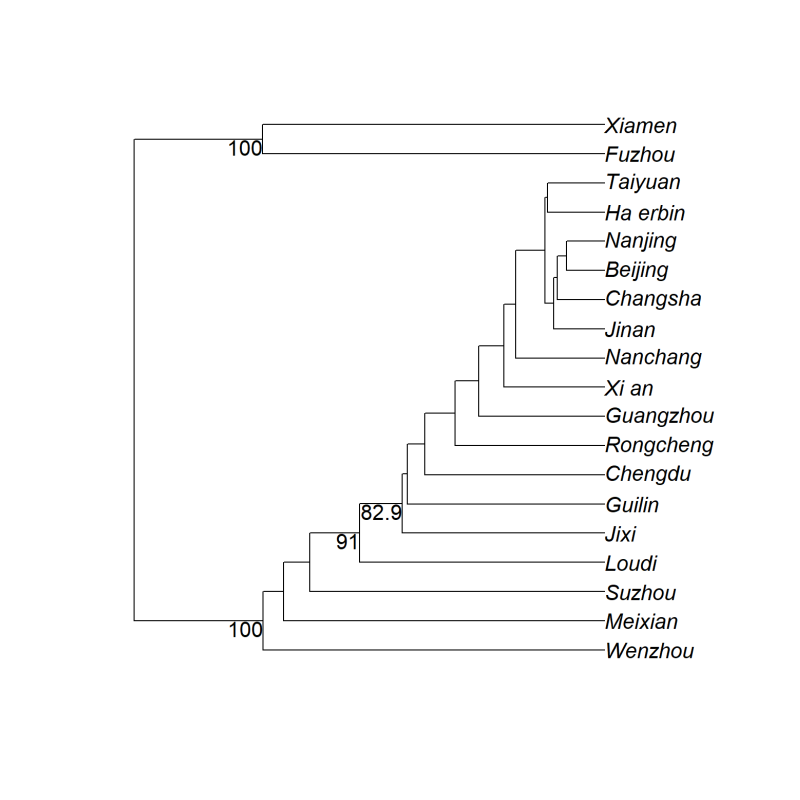
\includegraphics[scale=.4]{Figure/UPGMA_BS_with}
\caption{Avec emprunts}
\end{subfigure}
\begin{subfigure}{.5\textwidth}
\centering
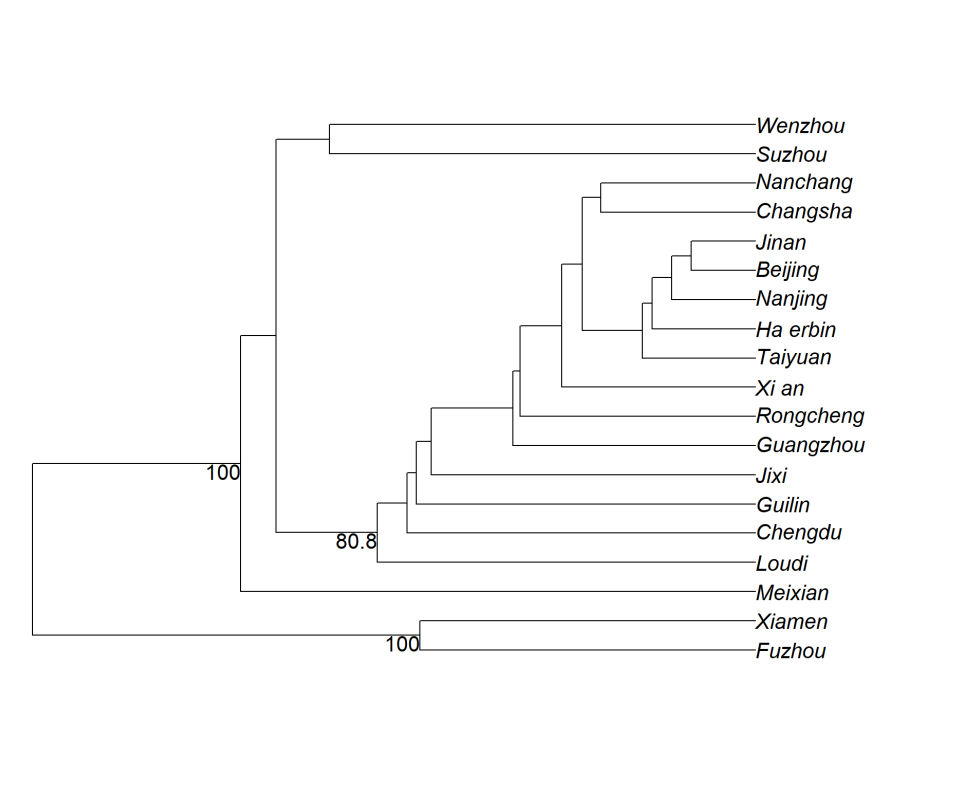
\includegraphics[scale=.4]{Figure/UPGMA_BS_without}
\caption{Sans emprunts}
\end{subfigure}
\caption{Arbres d'UPGMA testés avec la technique de BS}
\label{Fig:UPGMA_BS}
\end{figure}

\subsection{La méthode d'NJ}
On obtient deux arbres non enracinés avec la méthode d'NJ, avec ou sans emprunts, dans la figure \ref{Fig:NJ}. Dans tous les deux arbres, on peut bien observer les relations entre les variantes. Généralement, les variantes du mandarin (y compris le Jin de Taiyuan) se présentent assez proche l'une de l'autre, entourées par les variantes non mandarin. Les positions du Yue de Guangzhou dans toutes les deux conditions sont toujours proches des variantes du mandarin. Les Wu de Suzhou et Wenzhou, comme les Min de Fuzhou et Xiamen, sont toujours assez proches.

\begin{figure}[htbp]
\flushleft
\begin{subfigure}{.5\textwidth}
\centering
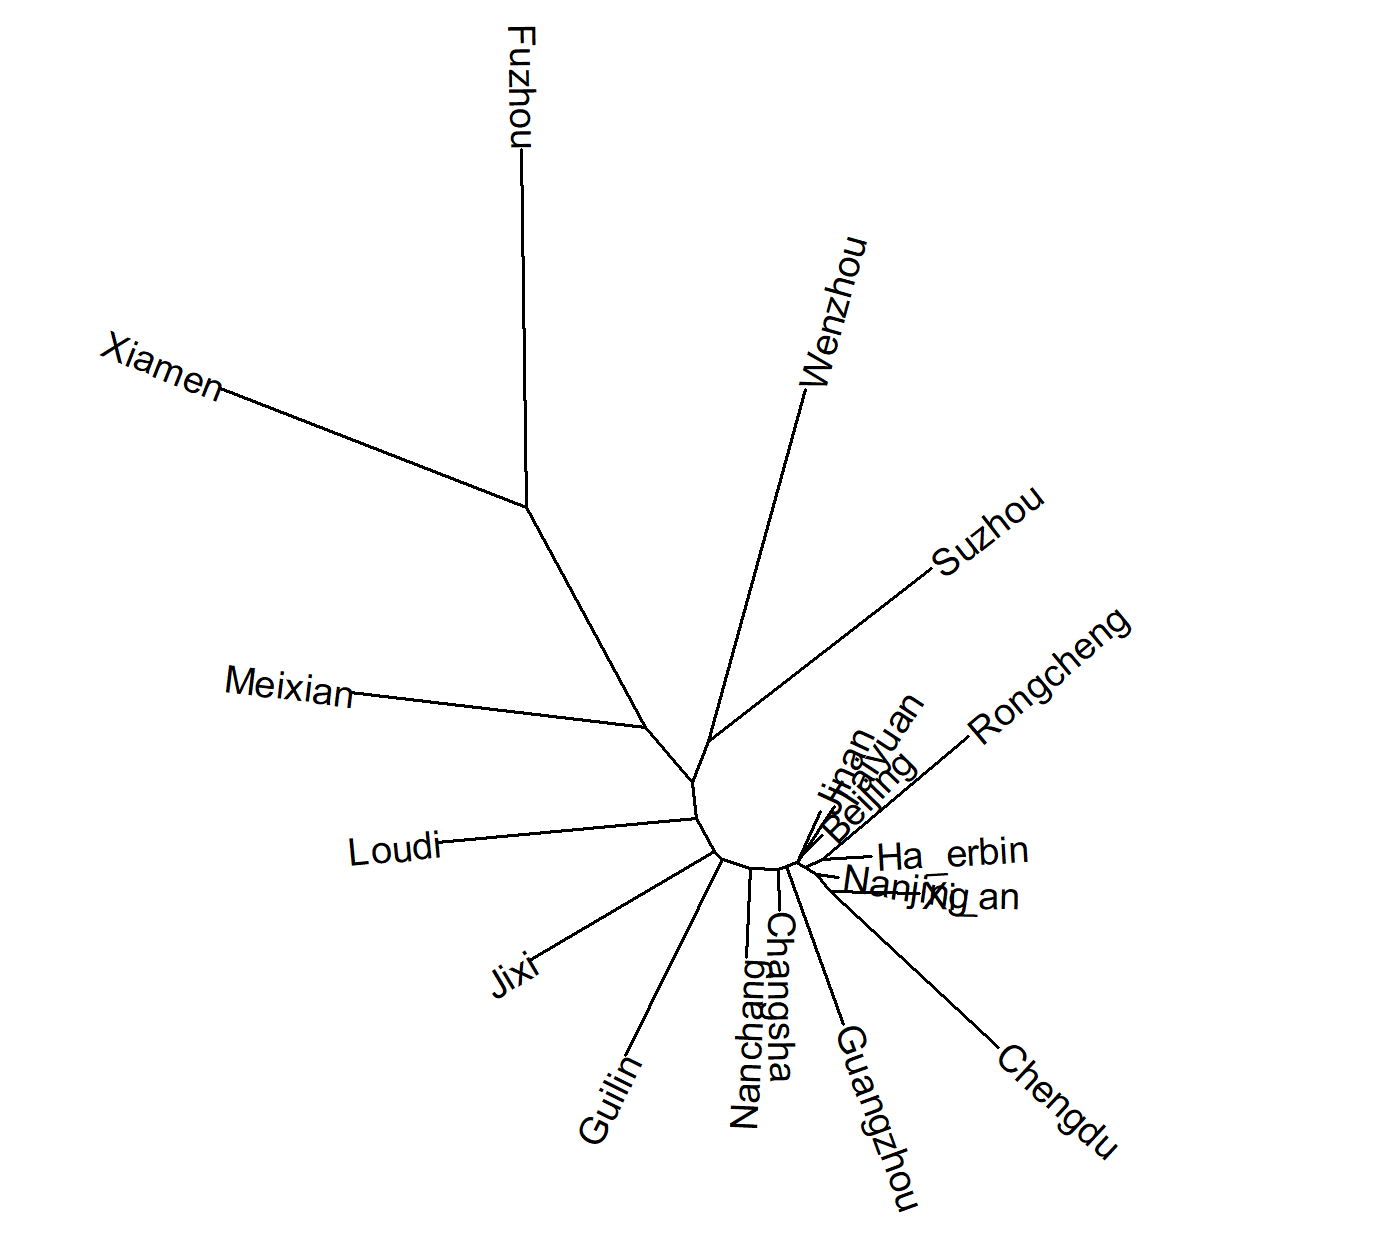
\includegraphics[scale=.25]{Figure/NJ_with}
\caption{Avec emprunts}
\end{subfigure}
\begin{subfigure}{.5\textwidth}
\centering
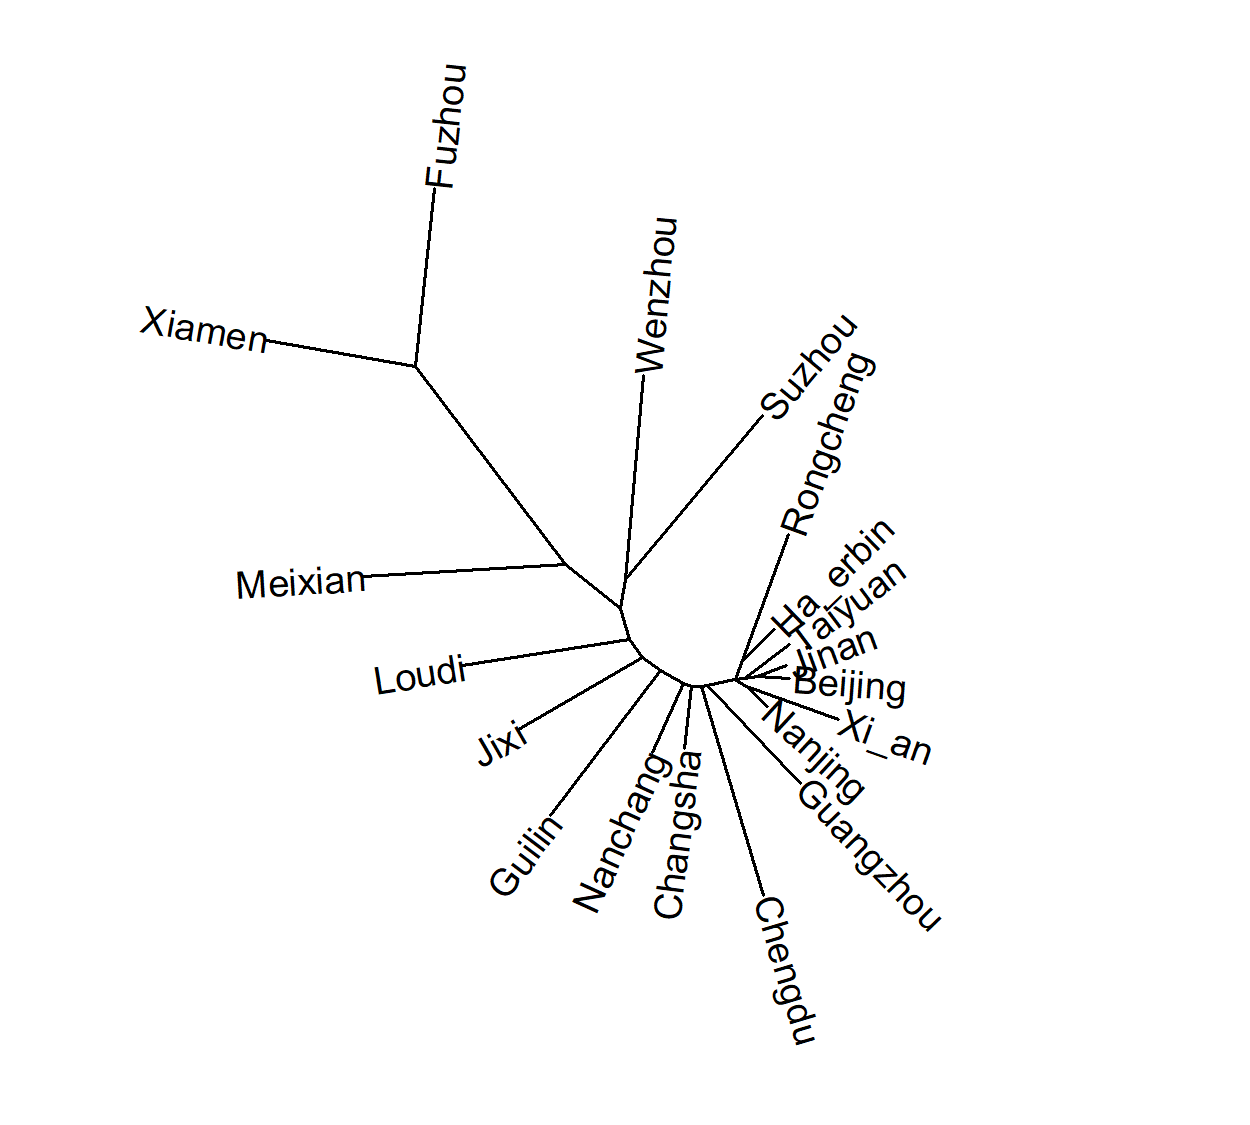
\includegraphics[scale=.3]{Figure/NJ_without}
\caption{Sans emprunts}
\end{subfigure}
\caption{Arbres générés avec la méthode d'NJ}
\label{Fig:NJ}
\end{figure}

\subsection{La méthode du maximum de parcimonie}
On obtient deux arbres racinés avec la méthode d'MP, avec ou sans emprunts, testés par la technique de bootstrap dans la figure \ref{Fig:MPR}. Les arbres proviennent de la technique de Ratchet, une méthode heuristique qui n'assure pas l'acquisition de l'arbre optimal mais l'arbre suboptimal. L'utilisation de cette méthode donnera souvent différents résultats chaque fois en fonction des détails du calcul. Mais certains points restent stables. On propose ici un des résultats du calcul. On racine les arbre en supposant que la variante Min de Xiamen soit le groupe externe. Dans tous les deux arbres, le Min de Fuzhou et le Hakka de Meixian sont toujours les deux premiers à se séparer après le Min de Xiamen. Les Wu de Suzhou et Wenzhou sont regroupés ensemble dans tous les deux arbres, mais leurs positions sont très différentes : dans l'arbre avec emprunts, ils sont séparés après le Hakka de Meixian, alors que dans l'arbre sans emprunts, ils sont séparés plus tard après le Hui de Jixi. Les Xiang de Changsha et Loudi n'appartiennent à un clade dans aucun arbre. Le Yue de Guangzhou est toujours proche des variantes du mandarin dans tous les deux arbres. Dans l'ensemble, les topologies des deux arbres générés avec la méthode d'MP sont assez différentes, ce qui semble impliquer que l'exclusion des emprunts influencerait la méthode d'MP. Puisque les topologies sont assez différentes, les valeurs de bootstrap ne compte pas beaucoup pour l'interprétation.

\begin{figure}[htbp]
\flushleft
\begin{subfigure}{.5\textwidth}
\centering
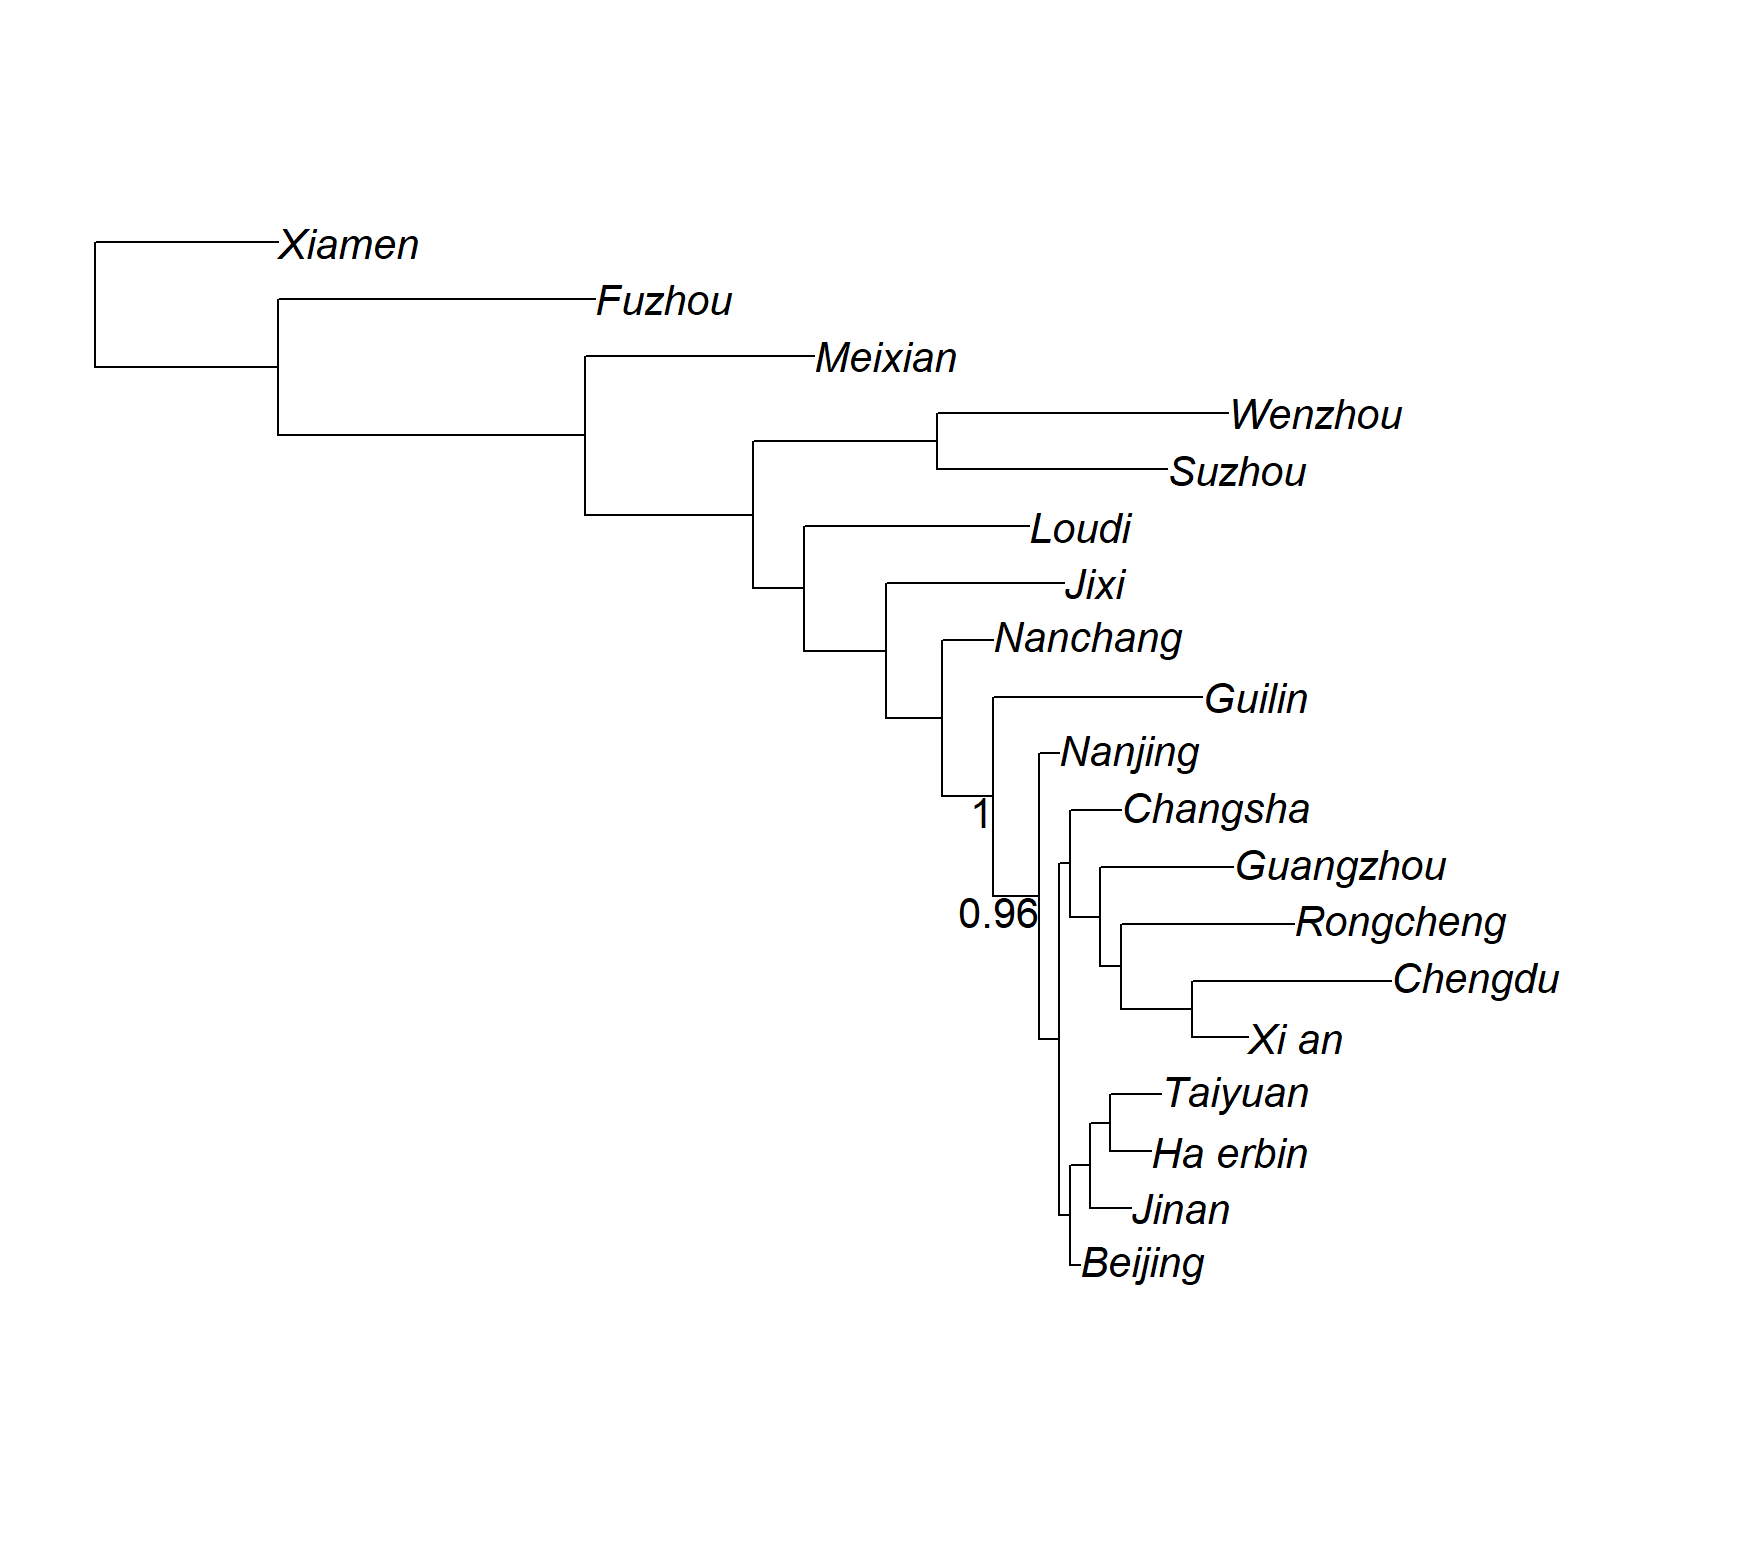
\includegraphics[scale=.2]{Figure/MPR_BS_with}
\caption{Avec emprunts}
\end{subfigure}

\begin{subfigure}{.5\textwidth}
\centering
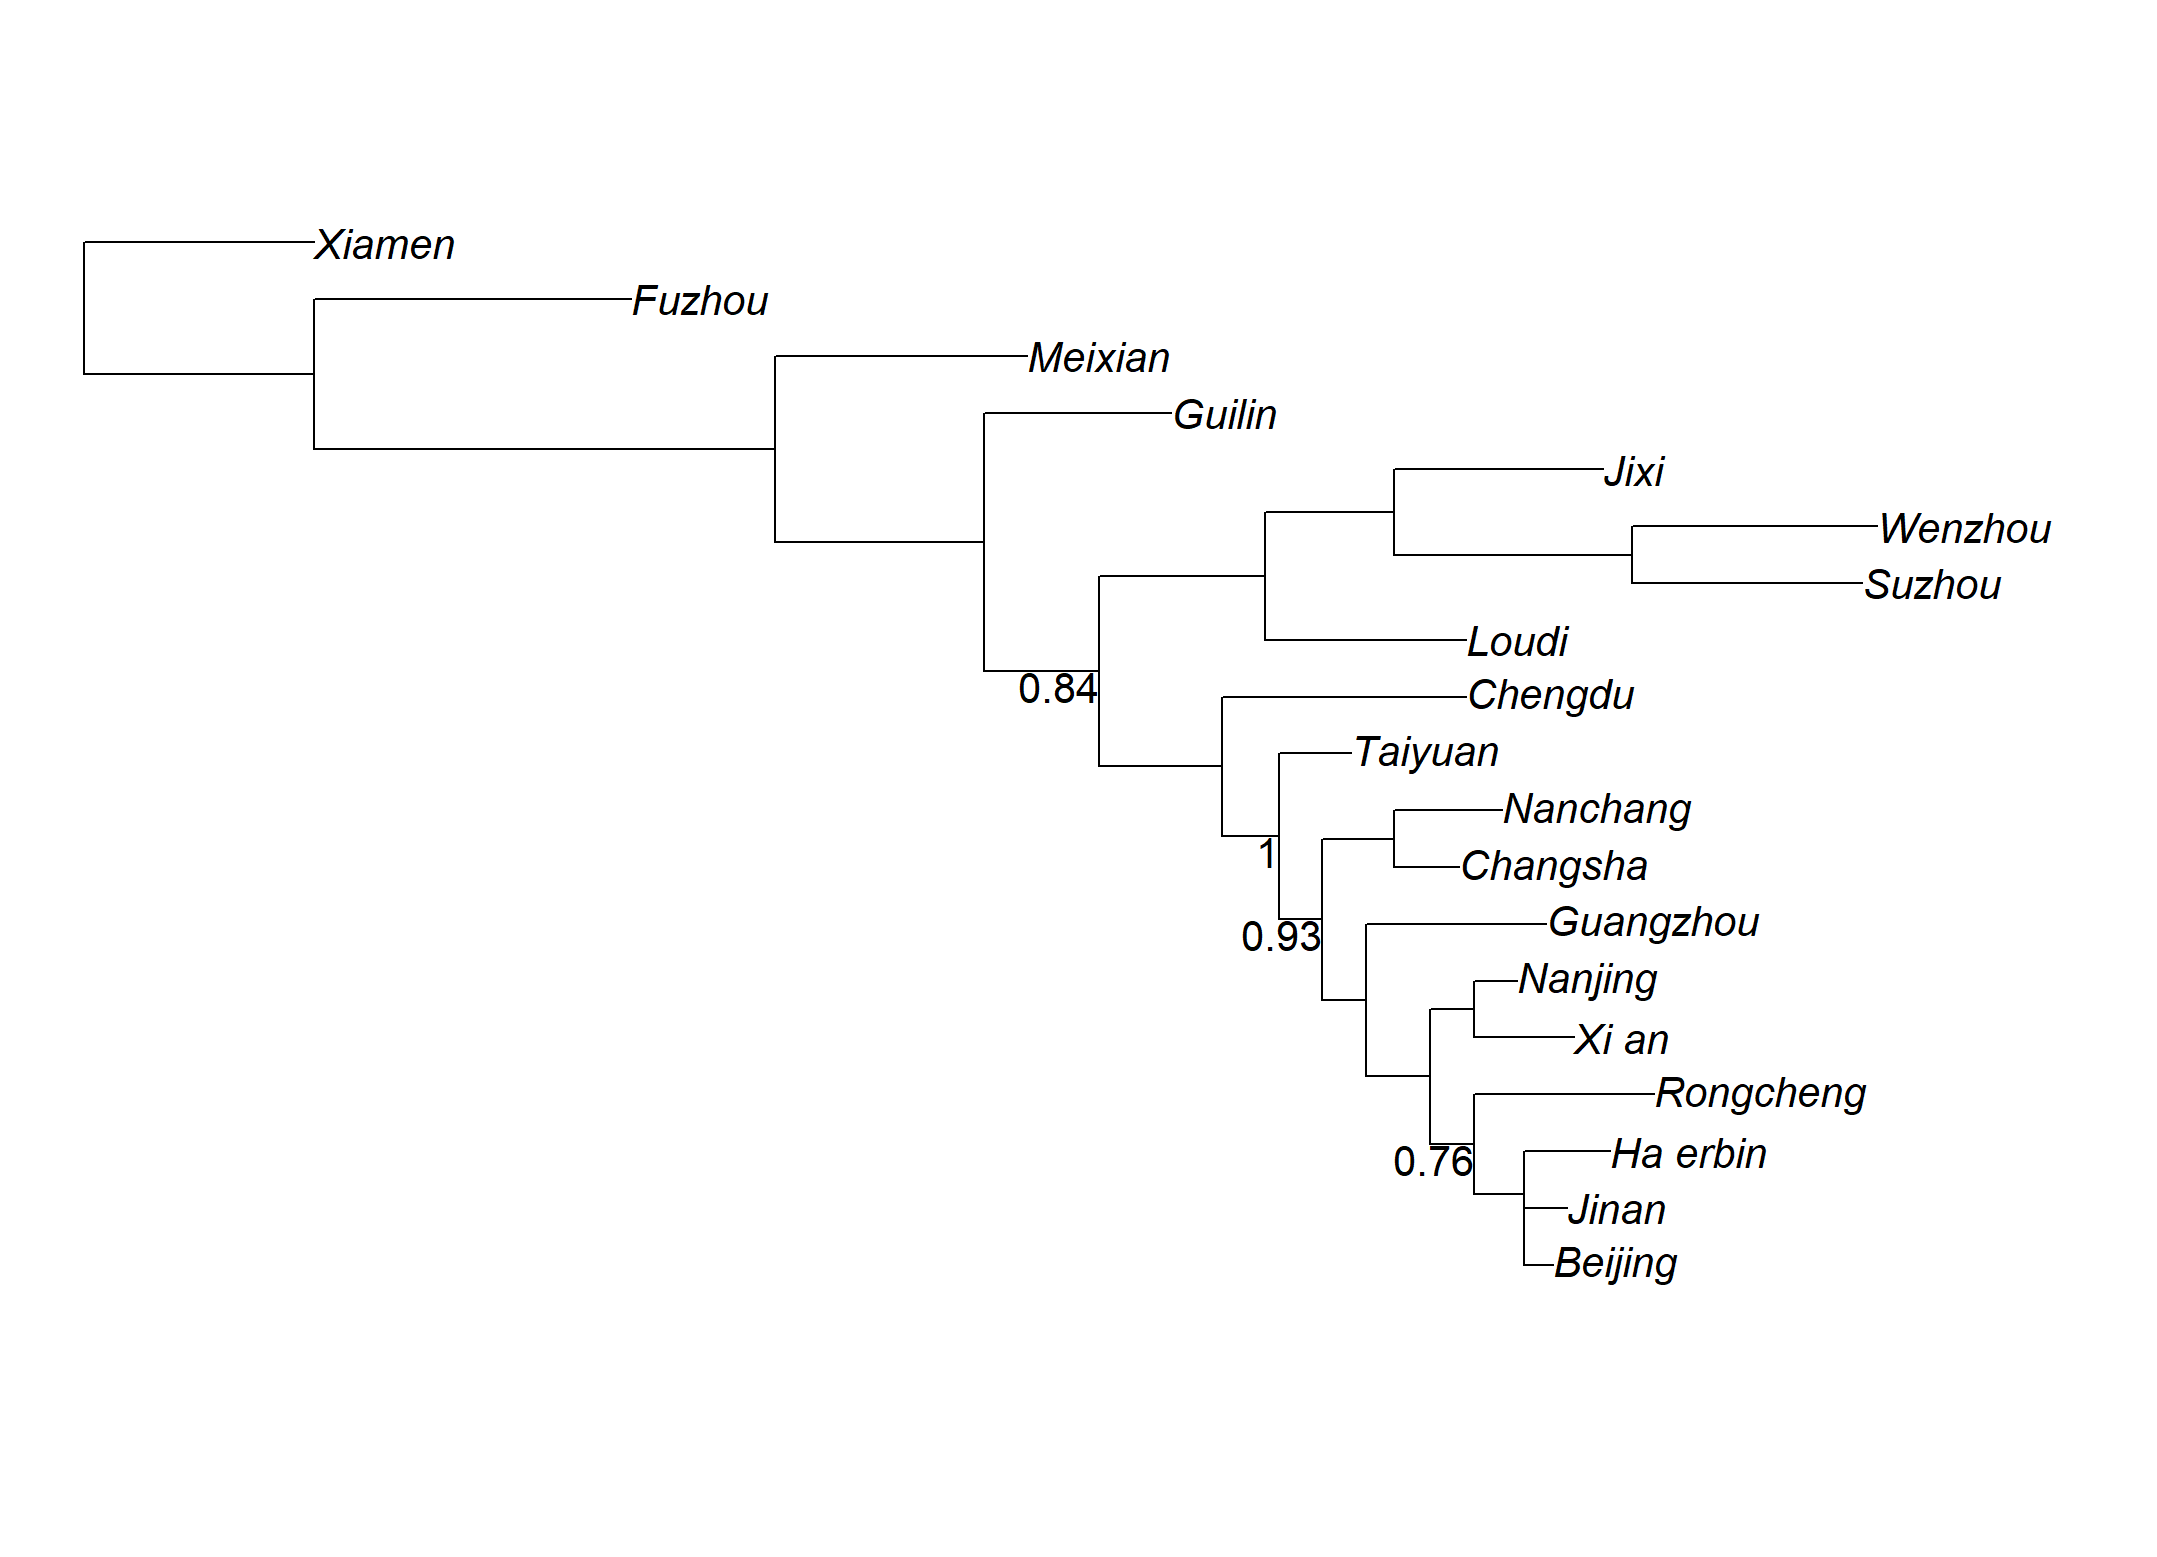
\includegraphics[scale=.2]{Figure/MPR_BS_without}
\caption{Sans emprunts}
\end{subfigure}
\caption{Arbres MPR testés avec la technique de BS}
\label{Fig:MPR}
\end{figure}

De l'autre part, on utilise la méthode de \textit{``branch and bound''} pour générer une série d'arbres non enracinés équitablement parcimonieux et obtient un arbre consensus strict à partir de ces arbres individus. Les deux arbres consensus stricts sont représentés dans la figure \ref{Fig:MPR_BAB}. On peut bien voir que dans la condition avec emprunts, il y a une forme en étoile sur un bout de l'arbre à cause de trop de divergences entre les arbres individus, alors que dans la condition sans emprunts, la situation s'améliore. Dans tous les deux arbres, on peut voir que le Yue de Guangzhou se trouve toujours proche des variantes du mandarin et le mandarin de Chengdu se trouve toujours loin d'autres variantes du mandarin. Dans tous les deux arbres, les Wu de Suzhou et Wenzhou sont assez proches comme les Min de Fuzhou et Xiamen. 

\begin{figure}[htbp]
\flushleft
\begin{subfigure}{.5\textwidth}
\centering
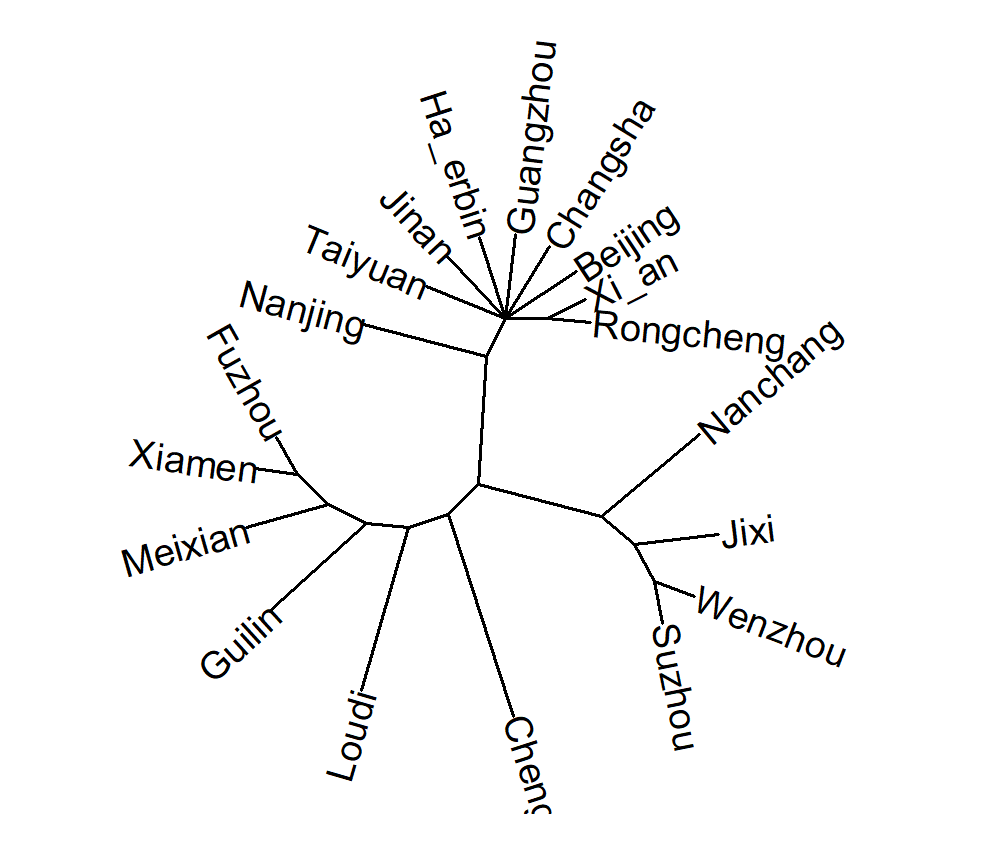
\includegraphics[scale=.4]{Figure/MP_bab_sc_with}
\caption{Avec emprunts}
\end{subfigure}
\begin{subfigure}{.5\textwidth}
\centering
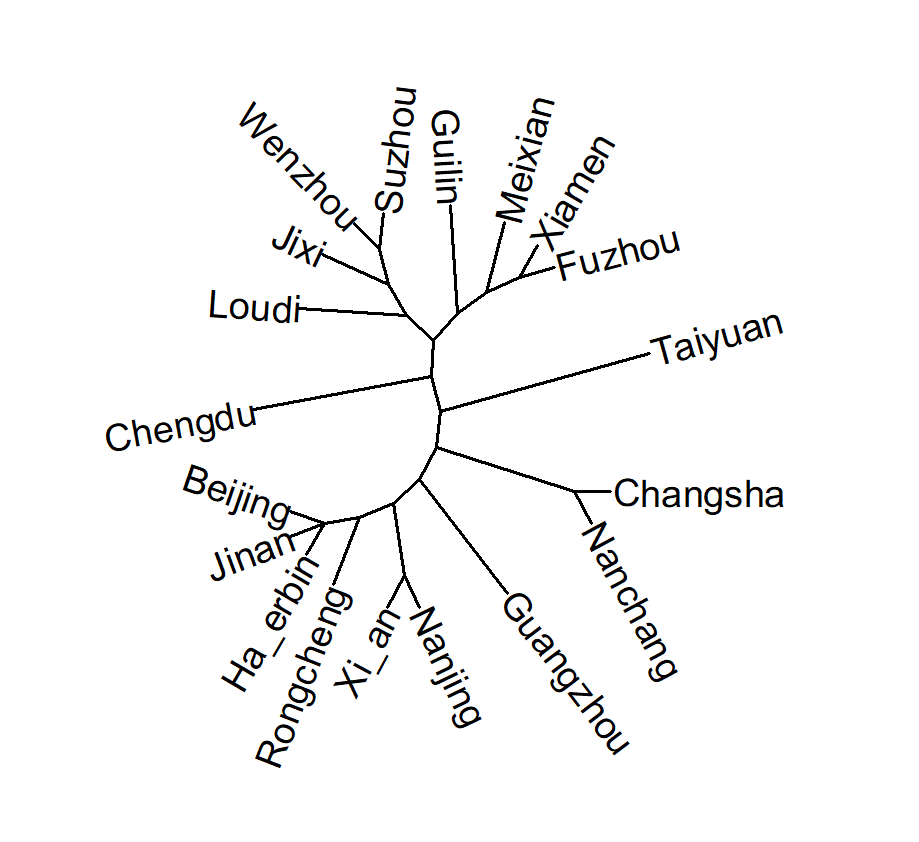
\includegraphics[scale=.4]{Figure/MP_bab_sc_without}
\caption{Sans emprunts}
\end{subfigure}
\caption{Arbres consensus strict des arbres MP}
\label{Fig:MPR_BAB}
\end{figure}

\section{Discussion}
Dans les résultats obtenus avec différentes méthodes phylogénétiques ci-dessus, il semble qu'on peut au moins dégager certaines observations préliminaires au sujet de l'influence des emprunts dans le calcul phylogénétique : l'exclusion des emprunts n'influence pas beaucoup les résultats obtenus avec les méthodes basées sur les distances, mais le fait en cas de la méthode du maximum de parcimonie. Elle atténue aussi les conflits entre les arbres individus quant à la génération de l'arbre consensus. De plus, il y a encore plusieurs points intéressants concernant la classification des variantes.

\subsection{Les Xiang de Changsha et Loudi}
A la différence des Min de Fuzhou et Xiamen et des Wu de Suzhou et Wenzhou, avec aucune méthode ont-on pu obtenir un arbre dans lequel les Xiang de Changsha et Loudi constituent un groupe monophylétique ou du moins sont assez proches. Le Xiang de Changsha est toujours plus proche des variantes du mandarin que le Xiang de Loudi. Cela confirme la classification traditionnelle du Xiang : la distinction entre le ``Xiang ancien'' (老湘語) relativement conservateur, représenté par Loudi et le ``Xiang nouveau'' (新湘語) relativement innovateur, représenté par Changsha. Le fait que ces deux variantes ne constituent pas un clade peut s'expliquer par l'influence intense du mandarin sur le Xiang de Changsha vu son statut important en tant que centre administratif de la province du Huhan, ainsi qu'il a perdu beaucoup de caractéristiques propres au Xiang.

\subsection{Le Hakka de Meixian et le Gan de Nanchang}
Même si beaucoup de savants ont l'habitude de mettre le Hakka et le Gan ensemble dans la discussion avec le terme ``客贛方言'', les résultats phylogénétiques semblent contredire cette pratique. Le Gan de Nanchang est toujours beaucoup plus innovateur que le Hakka de Meixian, des fois enchassé dans les variantes du mandarin, alors que le Hakka de Meixian a tendance à rester assez archaïque, toujours séparé après le Min. \textcite[361]{Norman2003kejia} pense que le Hakka a généralement deux grandes couches, une couche archaïque partageant des points communs avec le Min et une couche récente partageant des points communs avec le Gan. Les résultats phyogénétiques ici semblent refléter la caractéristique de la couche archaïque du Hakka, ce qui est pertinent sous la perspective de la stratification. 

\subsection{Le Yue de Guangzhou et le mandarin de Chengdu}
Dans presque tous les résultats phylogénétiques, les statuts du Yue de Guangzhou et du mandarin de Chengdu peuvent poser la question : le Yue de Guangzhou est proche des variantes du mandarin et des fois enchassé dedans. Par contre, le mandarin de Chengdu reste souvent loin d'autres variantes du mandarin. 

Un point méthodologique peut être proposé pour expliquer ce phénomène. Dans les enquêtes sur le terrain auprès des langues sinitiques, il arrive que tant les enquêteurs que les informateurs dépendent beaucoup sur l'écriture pour acquérir les données. La même situation arrive aux données collectées par \textcite{Liu2007hexinci}. Ils listent en même temps les concepts en anglais et en chinois (mandarin standard) dans leur ouvrage. Mais il est imaginable que les enquêteurs/informateurs chinois ne compteraient pas sur l'anglais pour dégager les matériaux. Il est donc probable que les informateurs subissent l'influence de l'écriture et donne la prononciation ``littérale'' (et probablement littéraire) d'un concept selon son écriture. Dans les deux conditions avec ou sans emprunts, on calcule pour chaque variante dans notre base de données les rapports des entrées partageant les mêmes formes que les concepts en chinois en supposant qu'au moin une partie de ces entrées soient directement lues selon l'écriture des concepts par les informateurs. Les rapports des variantes sont montrés dans la table \ref{tab:rapport_litteral}. On peut bien voir que dans toutes les deux conditions, les valeurs sont différentes en fonctions des variantes. Mais dans l'ensemble, les variantes du mandarin possèdent des rapports plus hauts que les variantes non mandarin au sujet des entrées avec les mêmes formes que les concepts, ce qui est normal parce que les concepts s'expriment et donc s'écrivent selon le mandarin standard. Curieusement, on trouve que le Yue de Guangzhou possède ce rapport très haut comme les variantes du mandarin, alors que ce rapport du mandarin de Chengdu se montre relativement bas par rapport à d'autres variantes du mandarin, même si à certaines variantes non mandarin. On peut supposer donc que les données du Yue de Guangzhou soient moins crédibles dans notre base de données parce qu'elles proviennent peut-être des prononciations littérales de l'écriture des concepts par l'informateur. Un exemple est le concept ``152. give'' (給). Dans la base de données, l'entrée du Yue de Guangzhou partage la même forme que le concept : 給[kʰɐpD1] (\cite[51]{Liu2007hexinci}), alors qu'il est bien connu que dans le Yue de Guangzhou, on exprimera cette notion plutôt avec le verbe ``畀[peiC1/B1]'' (\cite[137]{Bai1998Guangzhou}). Même si ce concept a été exclu d'emblée dans notre calcul, il reste sûrement beaucoup d'autres entrées de ce type qu'on est pas arrivé à exclure, qui induit en erreur les résultats.

Pour le mandarin de Chengdu, cela peut s'expliquer par la même motivation, càd. que certains informateurs ne seraient pas influencés par l'écriture, mais prétendraient aux expressions toutes différentes de l'écriture des concepts. Certaines de ces expressions pourraient apprtenir à différents registres qu'on est pas arrivé à exclure un par un, ce qui pourrait aussi causer un biais vers les résultats. Ce phénomène implique qu'il faut bien considérer les méthodes pour effectuer les enquêtes afin d'obtenir des matériaux pertinents.

% Table generated by Excel2LaTeX from sheet '字面读音比例'
\begin{table}[htbp]
  \centering

    \begin{tabular}{lll}
    \toprule
          & \multicolumn{1}{l}{Avec emprunts} & \multicolumn{1}{l}{Sans emprunts} \\
    \midrule
    Beijing    & 76\%  & 76\% \\
    Jinan      & 74\%  & 75\% \\
    Guangzhou  & \cellcolor[rgb]{ .851,  .851,  .851}70\% & \cellcolor[rgb]{ .851,  .851,  .851}69\% \\
    Rongcheng  & 69\%  & 68\% \\
    Ha\_erbin   & 68\%  & 68\% \\
    Nanjing    & 68\%  & 69\% \\
    Taiyuan    & 67\%  & 67\% \\
    Xi\_an      & 65\%  & 65\% \\
    Guilin     & 64\%  & 64\% \\
    \midrule
    Changsha   & 62\%  & 59\% \\
    Nanchang   & 62\%  & 59\% \\
    Jixi       & 61\%  & 61\% \\
    Loudi      & 58\%  & 58\% \\
    Chengdu    & \cellcolor[rgb]{ .851,  .851,  .851}56\% & \cellcolor[rgb]{ .851,  .851,  .851}55\% \\
    Suzhou     & 54\%  & 53\% \\
    \midrule
    Meixian    & 52\%  & 51\% \\
    Wenzhou    & 50\%  & 51\% \\
    Xiamen     & 40\%  & 36\% \\
    Fuzhou     & 22\%  & 32\% \\
    \bottomrule
    \end{tabular}%
  \caption{Rapports des entrées avec les mêmes formes que les concepts}
  \label{tab:rapport_litteral}%
\end{table}%

\subsection{Nativisation des emprunts}
Il y a une autre explication pour la question du Yue de Guangzhou dans la partie précédente, mais ce phénomène peut arriver à n'importe quelle variante.

La \textbf{nativisation étymologique des emprunts''} (en anglais ``etymological nativisation of loanwords'') est un type spécial d'analogie dans le contact linguistique proposée par \textcite{aikio2007etymological}. Précisément, quand les locuteurs d'une langue empruntent des mots d'une autre langue généalogiquement assez proche (même non apparentée), si les locuteurs se rendent compte, même si d'une façon intuitive, des correspondances régulières entre certaines catégories phonologiques de ces deux langues en contact, ils substitueraient les catégories phonologiques de la langue d'arrivée à celles de la langue donneuse dans les emprunts sur la base de ces correspondances obtenues intuitivement au lieu d'adopter les catégories phonologiques de la langue d'arrivée similaires à celles de la langue donneuse au niveau de la perception. Il s'ensuit que les emprunts émergeant de cette façon posséderaient des traits apparemment propres à la langue d'arrivéé qui les rendent plus anciens qu'ils ne le soit. Le pire, cela induirait en erreur l'identification d'origine de ces emprunts en faisant risquer de les considérer comme des mots hérités de la langue d'arrivée et comme des mots apparentés avec la langue donneuse. 

Prenons comme exemple le concept ``54. sun'' (太陽). Dans la base de données, les variantes expriment ce concept généralement par deux formes : soit 太陽, soit 日頭 (ou 熱頭 dans d'autres ouvrages), ou leurs formes dérivées. Certaines variantes utilisent toutes les deux. Le Yue de Guangzhou utilise la forme 太陽 (\cite[98]{Liu2007hexinci}). Mais selon \textcite[389]{Zhan2002yue}, beaucoup de variantes du Yue, y compris Guangzhou, utilisent plutôt 熱頭/日頭. Le même cas arrive au Wu de Suzhou (\cite[346]{Ye1988suzhou_fangyanzhi}) qui utilise en même temps 太陽 et 日頭, mais dans la base de données seule la forme 太陽 a été fournie. Puisque ces emprunts ne peuvent pas être détectés selon les correpondances phonologiques, une solution possible est de consulter les documentations du lexique des variantes, ou alors de choisir au début une variante subissant moins d'influences de l'extérieur.

\chapter{Conclusion}
Dans ce mémoire, au niveau de la méthodologie, on généralise abord les critères de la stratification au niveau de la détermination d'une couche et de la détermination de la chronologie des couches (\ref{critr_strat}), sur la base de la discussion de la connotation du terme traditionnel dans la dialectologie chinoise ``wen-bai'' et de ses insuffisances (\ref{wenbai}). On discute aussi trois questions concernant la pratique de la stratification en proposant notre solution ou explication (\ref{question_strat}). Ensuite, on applique ces critères à trois cas d'études (\ref{cas_etudes}) pour montrer la complexité des questions des couches. Puis, on généralise à partir des ouvrages des savants les critères concrets pour distinguer les couches de chaque variante (\ref{couche_dialect}). 

Au niveau des données, ces critères précédents, tant généraux que concrets, sont employés pour annoter les couches des syllabes dans la base de données déjà établie. Après la correction et le traitement des données, on obtient deux versions de données : une série de COGIDs pleines avec emprunts et une autre série de COGIDs pleines sans emprunts à passer aux codes des méthodes phélogénétiques (\ref{database}). 

Au niveau de la technique, on utilise principalement la méthode d'UPGMA, la méthode d'NJ et la méthode du maximum de parcimonie pour générer différents arbres enracinés ou non enracinés, à partir desquels sont discutés les résultats phylogénétiques et leurs inspirations (\ref{phylo}). 

Pour conclure, l'exclusion des emprunts influence dans différentes mesures les résultats phylogénétiques, qui confirment dans une certaine mesure la classification traditionnelle des langues sinitiques et l'arbre phylogénétique établi par \textcite{sagart2011classifying} et révèle en même temps certains points apparemment anormaux. Précisément, il faut bien veiller à la méthodologie pendant les enquêtes sur le terrain pour collecter les données pertinentes et au phénomène de la nativisation des emprunts qui cause des emprunts non détectables, tous deux risquant d'induire en erreur les résultats phylogénétiques. 

Dans le futur, il y a plusieurs directions principales des travaux plus profonds : (1) la généralisation plus raffinée de la typologie des couches des langues sinitiques pour bien distinguer les mots hérités et les emprunts ; (2) les études des cas spécifiques de l'irrégularité sporadique des syllabes, ce qui peut impliquer des informations inspiratrices; (3) l'identification de l'étymologie opaque des mots problématiques, qui appartiennent souvent à la couche archaïque ou à la substrate ; (4) la consultation des littératures sur le lexique et l'histoire lexicale des langues sinitiques ; (5) l'application des méthodes phylogénétiques plus avancées aux données des langues sinitiques ; (6) la référence aux documentations d'autres domaines, comme l'archéologie, la génétique, la statistique, l'histoire de migration, etc.





\newpage
\chapter*{Bibliographie}
\addcontentsline{toc}{chapter}{Bibliographie}
\printbibliography[heading=none]

\newpage
%\chapter*{Appendice}
%\addcontentsline{toc}{chapter}{Appendice}

\begin{appendices}

\chapter{Morphèmes grammaticaux}\label{appendice1}
Quand le morphème grammatical est présent dans beaucoup de variantes pour un concept, on ne liste pas les variantes entre parenthèses. Les syllabes sans caractères pertinents sont représentées directement par leurs prononciations entre crochets.

% Table generated by Excel2LaTeX from sheet '虚词'
\begin{longtable}[htbp]{lll}
    \endfirsthead
	
	\multicolumn{3}{c}{Table continuée}\\
    \toprule
    Numéro & Concept & Morphème grammatical \\
    \hline
    \endhead

    \hline
    \multicolumn{3}{r}{à continuer} \\
    %\hline
    \endfoot
    \endlastfoot
    
    \toprule
    Numéro & Concept & Affixe grammatical \\
    \midrule
    1     & vomit & 了 ; 嘞 (Taiyuan) \\
    3     & skin  & 子 \\
    4     & float & [lɛ] (Fuzhou) ; 倒 (Guilin) \\
    6     & wife  & 子 ; 的 ; 們 \\
    7     & all   & 下 (Fuzhou) \\
    13    & nose  & \makecell[l]{子 ; 哥 (Guangzhou) ; 頭 ; \\公 (Meixian) ; 仔 (Xiamen)} \\
    14    & ice   & 子 \\
    15    & neck  & 子 \\
    23    & breasts & 子 ; 仔 (Xiamen) \\
    25    & woods & 子 \\
    27    & sand  & 子 ; 兒 (Meixian) \\
    31    & tongue & 子 ; 頭 ; 嫲 (Meixian) \\
    32    & snake & 老 (Fuzhou) ; 哥 (Meixian) \\
    33    & rope  & 子 ; 仔 (Xiamen) \\
    34    & louse & 子 ; 嫲 (Meixian) \\
    36    & what  & 子 ; 個 (Meixian) \\
    37    & stone & 頭 ; 子 ; 兒 \\
    38    & hand  & 子 \\
    39    & tree  & 兒 (Meixian) \\
    45    & fruit & 子 ; 們 (Rongcheng) \\
    54    & sun   & 頭 \\
    55    & lie   & 倒 (Chengdu) ; 起 (Chengdu) \\
    57    & sky   & 上 ; 中 (Fuzhou) ; 里 (Wenzhou) \\
    59    & head  & 那 (Meixian) ; 得 (Taiyuan) \\
    60    & hair  & 那 (Meixian) \\
    64    & leg   & 子 \\
    67    & night & \makecell[l]{上 ; 子 ; 了 (Chengdu) ; \\下 ; 裏 (Loudi) ; 裏向 (Suzhou) ; \\咧 (Xi'an)} \\
    68    & tail  & 巴 ; 子 ; 兒 (Wenzhou) \\
    74    & knee  & 頭 ; 額 (Changhsa) ; 克 (Chengdu, Xi'an) ;  \\
    91    & leaf  & 子 ; 兒 \\
    96    & fish  & [tsɿ] [te] (Guilin) \\
    101   & moon  & 巴巴 (Changsha) \\
    108   & husband & \makecell[l]{老 ; 的 (Chengdu, Haerbin) ; 子 ; \\們 (Haerbin)} \\
    139   & belly & 子 \\
    143   & ear   & 仔 (Guangzhou, Xiamen) ; 公 (Meixian) \\
    148   & rotten & 了 (Rongcheng) ; 起 (Wenzhou) \\
    149   & father & 依 (Fuzhou) ; 阿 (Meixian) \\
    153   & root  & 子 \\
    154   & dog   & 囝 (Fuzhou) \\
    155   & bone  & 頭 ; 都 (Xi'an] \\
    156   & stick & 子 ; 兒 (Meixian, Wenzhou) \\
    157   & child & \makecell[l]{子 ; 兒 ; 哥 (Fuhzhou) ; \\個 (Loudi) ; 仔 (Xiamen)} \\
    169   & flower & 兒 (Jixi, Meixian) ; 仔 (Xiamen) \\
    173   & live (alive) & \makecell[l]{着 ; 的 ; 其 (Fuzhou) ; \\嘅 (Guangzhou) ; 個} \\
    180   & near  & 兜 (Fuzhou) \\
    194   & mather[sic] & 阿 (Xiamen) ; 老 (Xiamen) \\    
    196   & where & 兒 (Meixian) \\
    198   & there & 兒 (Jixi, Meixian) \\
    201   & year  & 頭 (Xiamen) \\
    202   & bird  & 兒 (Wenzhou) \\
    203   & woman & \makecell[l]{的 (Changsha, Chengdu) ; 伊 (Fuzhou) ; \\界 (Fuzhou) ; 們 (Haerbin) ; 仂 (Jixi) ; \\兒 (Meixian)} \\
    \bottomrule
  \caption{Morphèmes grammaticaux}
  \label{tab:addlabel}%
\end{longtable}%

\chapter{Morphèmes lexicaux secondaires}\label{appendice2}

% Table generated by Excel2LaTeX from sheet '次要实词'
\begin{longtable}[htbp]{lll}
    \endfirsthead
	
	\multicolumn{3}{c}{Table continuée}\\
    \toprule
    Numéro & Concept & Morphème lexical secondaire \\
    \hline
    \endhead

    \hline
    \multicolumn{3}{r}{à continuer} \\
    %\hline
    \endfoot
    \endlastfoot
    
    \toprule
    Numéro & Concept & Morphème lexical secondaire \\
    \midrule
    1     & vomit & \makecell[l]{發 (Chengdu) ; \\帶 (Loudi)} \\
    14    & ice   & 構 (Loudi) \\
    27    & sand  & 婆 (Changsha) \\
    31    & tongue & 喙 (Fuzhou) \\
    32    & snake & 老二 (Chengdu) \\
    34    & louse & \makecell[l]{母 (Fuzhou) ; \\婆 (Changsha, Loudi) ; \\跳 (Suzhou) ; \\家 (Xiamen)} \\
    36    & what  & 嘢 (Guangzhou) \\
    37    & stone & 塊 (Loudi) \\
    38    & hand  & 把 (Changsha) \\
    49    & split & \makecell[l]{裂 ; \\開 (Chengdu, Meixian) ; \\破 (Guilin, Loudi) ; \\爛 (Xi'an)} \\
    54    & sun   & \makecell[l]{窠 (Loudi) ; \\爺 (Xi'an)} \\
    57    & sky   & \makecell[l]{老爺 (Suzhou) ; \\頂 (Xiamen)} \\
    64    & leg   & \makecell[l]{把 (Changsha) ; \\肚 (Guilin)} \\
    67    & night & 間 (Changsha) \\
    74    & knee  & 褲 (Nanjing) \\
	102   & cloud & 彩 (Haerbin) \\    
    106   & narrow & 窄 (Jixi) \\
    166   & thick & 實 (Guilin, Haerbin) \\
    173   & live (alive) & 絡 (Jixi) \\
    186   & come  & 走 (Wenzhou) \\
    201   & year  & 份 (Chengdu, Haerbin) \\
    \bottomrule
  \caption{Morphèmes lexicaux secondaires}
  \label{tab:addlabel}%
\end{longtable}%

\chapter{Morphème à étymologie opaque}\label{appendice3}

% Table generated by Excel2LaTeX from sheet '词源模糊'
\begin{longtable}[htbp]{lll}
    \endfirsthead
	
	\multicolumn{3}{c}{Table continuée}\\
    \toprule
    Numéro & Concept & Syllabe à éymologie opaque \\
    \hline
    \endhead

    \hline
    \multicolumn{3}{r}{à continuer} \\
    %\hline
    \endfoot
    \endlastfoot
    
    \toprule
    Numéro & Concept & Syllabe à éymologie opaque \\
    \midrule
    1     & vomit & [xwe] (Loudi) \\
    2     & fear  & 唬 (Wenzhou) \\
    6     & wife  & \makecell[l]{媽 (Fuzhou) ; \\嫗 (Jixi) ; \\安 (Wenzhou) 2 ; \\某 (Xiamen)2}  \\
    7     & all   & 個郎 (Fuzhou)2 \\
    10    & throw & \makecell[l]{甩 (Changsha, Chengdu) ; \\{[kœʔ]} (Fuzhou) ; \\抾 (Fuzhou) ; \\{[jɔ]} (Loudi) ; 厾 (Suzhou)} \\
    12    & back  & \makecell[l]{{[pʰiaŋ]} (Fuzhou) ; \\胛 (Xiamen)} \\
    14    & ice  & 棱 (Loudi) \\
    17    & not   & \makecell[l]{伓 (Fuzhou) ; \\唔 (Meixian)} \\
    18    & rub   & \makecell[l]{撖 (Fuzhou) ; \\汧 (Taiyuan)} \\
    21    & flesh & 肉 > [baʔ] (Xiamen) \\
    22    & if    & 若 > [nã] (Xiamen) \\
    23    & breasts & \makecell[l]{奶 > [nɛiŋ] (Fuzhou) ; \\奶 > [nĩ] (Xiamen)} \\
    32    & snake & 蛇 > [lie] (Fuzhou) \\
    43    & who   & 瞞 (Meixian)2 \\
    47    & suck  & \makecell[l]{唚 (Changsha, Loudi) ; \\哜 (Nanchang) ; \\吮 > [çy] (Rongcheng) ; \\呼 (Suzhou)} \\
    49    & split & \makecell[l]{[tsei] (Nanchang) ; \\㧸 (Suzhou) ; \\{[do] (Wenzhou)} ; \\攦 (Xiamen)} \\
    50    & die   & 瓜 (Changsha)2 \\
    59    & head  & [sɑ] (Xi'an) (颡sang4 ?) \\
    63    & push  & \makecell[l]{捵 (Fuzhou) ; \\{[søyŋ]} (Fuzhou) ; \\{[nɤŋ] (Loudi)} ; \\逃 (Wenzhou)} \\
    65    & dig   & \makecell[l]{{[lau]} (Wenzhou) ; \\摀 (Xiamen)} \\
    66    & play  & [tsʰit] 迌 (Xiamen) \\
    67    & night & 晌 (Rongcheng) \\
    85    & squeeze & [tsʰe] (Loudi) \\
    90    & bite  & [ŋa] (Loudi) \\
    92    & one   & 蜀 (Fuzhou)2 \\
    94    & swim  & \makecell[l]{{[vo]} (Jixi) ; \\淴 (Suzhou)} \\
    96    & fish  & [tsɿ] [te] (Guilin) \\
    103   & in    & 勒 (Suzhou)2 \\
    104   & dirty & \makecell[l]{{[lo]} (Jixi) ; \\{[pʰa]} (Loudi) ; \\{[me]} (Meixian)} \\
    111   & know  & \makecell[l]{仈傳 (Fuzhou) ; \\知影 (Xiamen)} \\
    117   & scratch (>catch) & \makecell[l]{巴 (Chengdu)2 ; \\逮 (Chengdu)} \\
    119   & turn  & 擺 [lɛ] (Fuzhou) \\
    122   & leftside & \makecell[l]{济 (Suzhou)2 ; \\爿 (Xiamen)} \\
    126   & dust  & \makecell[l]{塕 (Fuzhou) ; \\坌 (Wenzhou)} \\
    127   & eat   & 歹 (Rongcheng)2 \\
    130   & blow  & \makecell[l]{{[pʰaŋ]} (Meixian) ; \\㖹 (Fuzhou, Xiamen)} \\
    131   & stab  & \makecell[l]{楠 (Rongcheng)2 ; \\頓 (Wenzhou)2} \\
    136   & dull  & \makecell[l]{瓜 (Chengdu)2 ; \\雛 (Fuzhou) ; \\愚 (Fuzhou) ; \\彪 (Rongcheng)2 ; \\歁 (Xiamen)} \\
    137   & fall  & \makecell[l]{逿 (Fuzhou) ; \\刷 (Loudi)2 ; \\特 (Suzhou)2} \\
    140   & short & [te] (Xiamen) \\
    142   & many  & 多 (Xiamen) \\
    148   & rotten & 飲 (Fuzhou) \\
    149   & father & \makecell[l]{{[mã]} (Guilin) ; \\達 (Xi'an)} \\
    152   & give  & \makecell[l]{{[tia]} (Guilin) ; \\{[xɑ̃]} (Jixi)} \\
    157   & child & \makecell[l]{噶 (Haerbin)2 ; \\娒 (Wenzhou) ; \\囝 (Xiamen)} \\
    160   & drink & 啉 (Xiamen) \\
    166   & thick & 賁 (Meixian)2 \\
    170   & bad   & \makecell[l]{痞 (Fuzhou, Xiamen) ; \\鄙 (Meixian) ; \\毛 (Wenzhou)} \\
    173   & live (alive) & [te] (Guilin) \\
    178   & foot  & [te] (Guilin) \\
    184   & tie   & \makecell[l]{{[diɔ̃]} (Loudi) ; \\{[tʰiaʔ]} (Nanchang)} \\
    185   & pull  & \makecell[l]{拉 > [lai] (Guangzhou) ; \\㧍 (Meixian)} \\
    188   & cold  & 凊 (Xiamen) \\
    190   & path  & 墿 (Fuzhou)2 \\
    192   & full  & 個郎 (Fuzhou) \\
    195   & hold-take & \makecell[l]{逮 (Chengdu) ; \\攞 (Guangzhou)} \\
    203   & woman & 娘 (Fuzhou) \\
    \bottomrule
  \caption{Syllabes à étymologie opaque}
  \label{tab:addlabel}%
\end{longtable}%

\chapter{Liens vers les données et les codes}\label{appendice4}

La base de donnée peut être consultée par le lien \url{http://lingulist.de/edictor/?file=liusinitic&remote_dbase=liusinitic2}.

Les codes utilisés pour corriger les données, filtrer les morphèmes non saillants, convertir les COGIDs partielles vers les COGIDs pleines et générer les résultats phylogénétiques peuvent être consultés par le lien \url{https://github.com/yuanyang11510/Dissertation-Master-Codes}. 

\end{appendices}

\backmatter
\tableofcontents
\listoftables
\listoffigures

\begin{verso}
\section*{Résumé}
%\blindtext
Ce mémoire a pour but de tester si l'exclusion des emprunts influencerait les résultats phylogénétiques des langues sinitiques et d'obtenir une impression préliminaire de ces résultats. Au niveau de la méthodologie, on discute de la connotation du terme traditionnel dans la dialectologie chinoise ``wen-bai'' et de ses insuffisances, sur la base du quoi sont généralisés les critères généraux et concrets de la stratification de 19 langues sinitiques d'une base de données déjà établie. Au niveau des données, ces critères précédents sont employés pour annoter les couches des syllabes des mots de cette base de données pour distinguer les mots hérités et les emprunts, afin d'obtenir deux séries de données avec ou sans emprunts. Au niveau de la technique, on applique principalement la méthode d'UPGMA, la méthode d'NJ et la méthode du maximum de parcimonie à ces deux séries de données pour discuter les résultats phylogénétiques et leurs inspirations. On trouve que l'exclusion des emprunts n'influence pas beaucoup les topologies générales des arbres UPGMA et NJ, mais le fait pour la méthode du maximum de parcimonie. Les résultats phylogénétiques confirme dans un degré la classification traditionnelle des langues sinitiques et révèle en même temps certains points apparemment anormaux. Il faut bien veiller à la méthodologie pendant les enquêtes sur le terrain pour collecter les données pertinentes et au phénomène de la nativisation des emprunts qui cause des emprunts non détectables, tous deux risquant d'induire en erreur les résultats phylogénétiques. Dans le futur, plus de travaux profonds méritent d'être effectués pour approfondir la phylogénie des langues sinitiques.

\noindent \textbf{Mots-clés:} langues sinitiques, stratification, phylogénie

\section*{Abstract}
%\blindtext
This thesis aims to test whether the exclusion of loanwords would influence the phylogenetic results of Sinitic languages and obtain a preliminary impression of these results. In terms of methodology, we discuss the connotation of the traditional term ``wen-bai'' in Chinese dialectology and its shortcomings, based on which general and specific criteria for the stratification of 19 Sinitic languages are generalized from an established database. At the data level, these criteria are employed to annotate the syllable layers of words in this database as to distinguish between inherited words and loanwords, in order to obtain two sets of data with or without loanwords. In terms of technique, we mainly use the UPGMA method, the NJ method, and the maximum parsimony method on these two sets of data to discuss the phylogenetic results and their insights. We find that the exclusion of loanwords does not significantly affect the general topologies of the UPGMA and NJ trees, but it does have an impact on the maximum parsimony method. The phylogenetic results confirm to some degree the traditional classification of Sinitic languages but also reveal certain apparently anomalous points. It is important to carefully consider the methodology during field investigations to collect relevant data as well as the phenomenon of loanword nativization, which can result in undetectable loanwords, both of which can potentially mislead phylogenetic results. In the future, further in-depth work deserves to be carried out to deepen the phylogeny of Sinitic languages.

\noindent \textbf{Keywords :} Sinitic languages, stratification, phylogeny
\end{verso}

\end{sloppypar}
\end{document}
